\documentclass[a4paper,12pt]{scrartcl}
\usepackage{a4wide}
\usepackage[left=2cm, right=2cm, top=3cm]{geometry}
\usepackage{graphics}
\usepackage{mathtools}
\usepackage{amsmath, amssymb} 
\usepackage[utf8]{inputenc}
\usepackage[ngerman]{babel}
\usepackage{hyperref}
\usepackage{enumitem}
\usepackage{booktabs}
\usepackage{aligned-overset}  % Um bei Align die Gleichheitszeichen übereinander zu haben
\usepackage[version=4]{mhchem}
\usepackage{cancel}
\usepackage{wrapfig}
\usepackage{marvosym}
\usepackage[headsepline]{scrlayer-scrpage}
\usepackage{subcaption}
\usepackage{tabularx}
\usepackage{environ}
\usepackage{natbib}
\usepackage{tikzsymbols}
\usepackage[skins, xparse, breakable]{tcolorbox}
\usepackage{xcolor}
\usepackage{dsfont}
\usepackage{pdfpages} % https://www.namsu.de/Extra/pakete/Pdfpages.html
\allowdisplaybreaks  % Damit Align-Umgebungen umgebrochen werden können



% Set to 1 (only selection) or 0 (full script)
\newcounter{reduce_to_selection}
\setcounter{reduce_to_selection}{0}
% \setcounter{reduce_to_selection}{1}
% \includeonly{Woche07}


\newcommand{\Tipps}[2]{
    \ifnum\value{reduce_to_selection}=1 {
        \subsection{Tipps zu den Aufgaben von Blatt #1}
        \Disclaimer{}\\
        #2
    }
    \fi
}



\bibpunct{[}{]}{;}{a}{}{,}
\usepackage{scalerel}
\def\stretchint#1{\vcenter{\hbox{\stretchto[440]{\displaystyle\int}{#1}}}}
\def\bs{\mkern-12mu}
\pagestyle{scrheadings}
\clearpairofpagestyles


\numberwithin{equation}{section}
\let\oldsection\section  % Footnotecounter resetten
\renewcommand{\section}{\setcounter{footnote}{0}\oldsection}
\renewcommand{\thefootnote}{\Roman{footnote}}
\setlist[itemize]{topsep=1pt, itemsep=0pt, parsep=0.5pt}  % Itemize manipulieren
\setlist[enumerate]{topsep=1pt, itemsep=0pt, parsep=0.5pt}  % Itemize manipulieren


%%%%%%%%%%%%%%%%%%%%%%%%%%%%% Neue Umgebungen
\NewEnviron{Answer}
{%
\noindent
\rotatebox[origin=c]{180}{%
\noindent
\begin{minipage}[t]{\linewidth}
\BODY
\end{minipage}%
}%
}%


\definecolor{mygreen}{RGB}{17,100,8}
\newtcolorbox[auto counter,number within=section]{Def}[2][]{%
breakable, enhanced, sharp corners, rounded corners=northwest, rounded corners=southeast, colback=blue!5!white,colframe=black!75!black,fonttitle=\bfseries,
title=Definition~\thetcbcounter: #2,#1}

\newtcolorbox[auto counter, number within=section]{Satz}[3][]{%
breakable, enhanced, sharp corners, rounded corners=southwest, rounded corners=northeast, colback=blue!5!white,colframe=red!75!black,fonttitle=\bfseries,
title=#2~\thetcbcounter: #3,#1}

\newtcolorbox[auto counter,number within=section]{Beispiel}[2][]{%
breakable, enhanced, colback=blue!5!white,colframe=blue!75!black, fonttitle=\bfseries,
title=Beispiel~\thetcbcounter: #2,#1}

\newtcolorbox[auto counter,number within=section]{Wiederholung}[2][]{%
breakable, enhanced, sharp corners, colback=green!5!white,colframe=mygreen!75!black, fonttitle=\bfseries,
title=Wiederholung~\thetcbcounter: #2,#1}

\makeatletter
\def\iddots{\mathinner{\mkern1mu\raise\p@
\vbox{\kern7\p@\hbox{.}}\mkern2mu
\raise4\p@\hbox{.}\mkern2mu\raise7\p@\hbox{.}\mkern1mu}}
\makeatother


\makeatletter
\newcommand{\tx}[1]{\text{#1}}
\newcommand{\Menge}[2]{\left\{#1\furdas#2\right\}}
\newcommand{\MengeDirekt}[1]{\left\{#1\right\}}
\newcommand{\diff}[2]{\frac{\text{d}#1}{\text{d}#2}}
\newcommand{\diffp}[2]{\frac{\partial#1}{\partial#2}}
\newcommand{\BiFo}[1]{\left\langle#1\right\rangle}
\newcommand{\Norm}[1]{\left|\left|#1\right|\right|}
\newcommand{\BiFoLeer}{\left\langle\cdot,\cdot\right\rangle}
\newcommand{\NormLeer}{\left|\left|\cdot\right|\right|}
\newcommand{\Spoiler}[1]{Hier werden wir nach Abgabe des Blattes den Lösungsweg skizzieren.}
\newcommand{\Matrix}[1]{\begin{pmatrix}#1\end{pmatrix}}
\newcommand{\MatrixAbs}[1]{\begin{vmatrix}#1\end{vmatrix}}
\newcommand{\MatrixInline}[1]{\left(\begin{smallmatrix}#1\end{smallmatrix}\right)}
\newcommand{\MatrixInvertieren}[2]{\left(\begin{matrix}#1\end{matrix}\,\left|\,\begin{matrix}#2\end{matrix}\right.\right)}
\newcommand{\Span}[2]{\text{span}\left\{#1\furdas#2\right\}}
\newcommand{\Spann}[1]{\text{span}\left\{#1\right\}}
\newcommand{\EinheitsN}{\mathds{1}_n}
\newcommand{\red}[1]{\textcolor{red}{\textbf{#1}}}
\newcommand{\blue}[1]{\textcolor{blue}{#1}}
\newcommand{\UausC}{Sei $U\subset\mathbb{C}$ offen}
\newcommand{\Res}{\text{Res}}
\newcommand{\qedsquare}{\hfill $\square$}
\newcommand{\qed}{\hfill \textbf{q.e.d.}}
\newcommand{\furdas}{\,|\,}
\newcommand{\mybox}[1]{\parbox[t]{8.5cm}{#1}}
\newcommand{\myboxU}[1]{\parbox[b]{8.5cm}{#1}}
\newcommand{\Zz}[1]{\textbf{Beh.}: \textbf{\textit{#1}}\\}
\newcommand{\Zb}[1]{\textbf{Bew.}: \blue{#1}\qedsquare}
\newcommand{\ZbOhne}[1]{\textbf{Bew.}: \blue{#1}}
\newcommand{\Skript}{\href{https://www.math.uni-hamburg.de/home/lentner/MfPh1/SkriptMfP1Lentner2020.pdf}{Skript}}
\newcommand{\Limes}[1]{\lim_{#1\rightarrow\infty}}
\newcommand{\LimesSum}[1]{\sum_{#1=0}^\infty}
\newcommand{\LimesSumOne}[1]{\sum_{#1=1}^\infty}
\newcommand{\LimesXiToX}{\lim_{\xi\to x}}
\newcommand{\SinusReihe}{\LimesSum{k}(-1)^k\frac{z^{2k+1}}{(2k+1)!}}
\newcommand{\KosinusReihe}{\LimesSum{k}(-1)^k\frac{z^{2k}}{(2k)!}}
\newcommand{\ExpReihe}[1]{\LimesSum{k}\frac{#1^{k}}{k!}}
\newcommand{\Cases}[1]{\begin{cases}#1\end{cases}}
\newcommand{\Id}{\text{Id}}
\newcommand{\BracedIn}[1]{\left({#1}\right)}
\newcommand{\BracedInSqr}[1]{\left[{#1}\right]}
\newcommand{\Abs}[1]{\left|{#1}\right|}
\newcommand{\artanh}{\text{artanh}}
\newcommand{\arsinh}{\text{arsinh}}
\newcommand{\arcosh}{\text{arcosh}}
\newcommand{\Disclaimer}{\textcolor{blue}{
$\left[\,\text{\parbox{0.95\textwidth}{\vspace{0.1cm}\textit{\textbf{Hinweis:}\\
Da wir euch offiziell nichts vorsagen sollen (was ja auch sinnvoll ist), sind die Tipps sehr allgemein gehalten. Hoffentlich helfen sie euch trotzdem, Ansätze zu finden, falls ihr mal nicht weiter kommt.\\
Bei konkreten Fragen helfen wir gerne persönlich.\vspace{0.1cm}}}}\,\right]$
}}
\newcommand{\Einleitung}[1]{\subsection*{Ausblick}
    \textcolor{blue}{\textit{#1}}}
\newcommand{\IV}{\text{IV}}
\newcommand{\im}{\text{im}}
\newcommand{\Abb}{\text{Abb}}
\newcommand{\Bij}{\text{Bij}}
\newcommand{\I}{\text{I}}
\newcommand{\II}{\text{II}}
\newcommand{\III}{\text{III}}
\newcommand{\card}{\text{card}}
\newcommand{\diag}{\text{diag}}
\newcommand{\grad}{\text{grad}}
\newcommand{\Hess}{\text{Hess}}
\newcommand{\rot}{\text{rot}}
\newcommand{\divv}{\text{div}}
\newcommand{\Diff}{\text{Diff}}
\newcommand{\Met}{\text{Mat}}
\newcommand{\Tr}{\text{Tr}}
\newcommand{\rg}{\text{rg}}
\newcommand{\End}{\text{End}}
\newcommand{\Aut}{\text{Aut}}
\newcommand{\GL}{\text{GL}}
\newcommand{\SL}{\text{SL}}
\newcommand{\ad}{\text{ad}}
\newcommand{\sgn}{\text{sgn}}
\makeatother
%%%%%%%%%%%%%%%%%%%%%%%%%%%%%%
\let\oldhref\href
\renewcommand{\href}[2]{\oldhref{#1}{\underline{\bfseries#2}}}
\renewcommand{\Re}{\text{Re}}
\renewcommand{\Im}{\text{Im}}
\newcommand{\rvec}{{\Vec{r}}}
\newcommand{\uvec}{{\Vec{u}}}
\newcommand{\pvec}{{\Vec{p}}}
\newcommand{\qvec}{{\Vec{q}}}
\newcommand{\jvec}{{\Vec{j}}}
\newcommand{\vvec}{{\Vec{v}}}
\newcommand{\fvec}{{\Vec{f}}}
\newcommand{\gvec}{{\Vec{g}}}
\newcommand{\hvec}{{\Vec{h}}}
\newcommand{\lvec}{{\Vec{l}}}
\newcommand{\evec}{{\Vec{e}}}
\newcommand{\yvec}{{\Vec{y}}}
\newcommand{\bvec}{{\Vec{b}}}
\newcommand{\cvec}{{\Vec{c}}}
\newcommand{\nablavec}{{\Vec{\nabla}}}
\newcommand{\alphavec}{{\Vec{\alpha}}}
\newcommand{\psivec}{{\Vec{\psi}}}
\newcommand{\varphivec}{{\Vec{\varphi}}}
\newcommand{\xivec}{{\Vec{\xi}}}
\newcommand{\avec}{{\Vec{a}}}
\newcommand{\svec}{{\Vec{s}}}
\newcommand{\nvec}{{\Vec{n}}}
\newcommand{\xvec}{{\Vec{x}}}
\newcommand{\Fvec}{{\Vec{F}}}
\newcommand{\Gvec}{{\Vec{G}}}
\newcommand{\wvec}{{\Vec{w}}}
\newcommand{\zvec}{{\Vec{z}}}
\newcommand{\dvec}{{\Vec{d}}}
\newcommand{\graph}{\text{graph}}
\newcommand{\Nullvec}{{\Vec{0}}}
\renewcommand{\Vec}[1]{{\text{\boldmath${#1}$}}}%\overset{_\rightharpoonup}

% \renewcommand{\Vec}[1]{{\mathbf{#1}}}%\overset{_\rightharpoonup}
\setlength{\parindent}{0pt}		 %Verhindert den automatischen Erstzeileneinzug



%%%%%%%%%%% Titel, Profs, Zeitraum etc.
\newcommand{\titel}{Tutorium zur Vorlesung\\
\textit{Mathematik II für Studierende der Geophysik/ Ozeanographie, Meteorologie und Physik}\\
SoSe 2022
}
\newcommand{\Kurztitel}{MfP2-Notizen}
\newcommand{\Zeitraum}{SoSe 2022}
\newcommand{\Profs}{zur Vorlesung von Dr. \textsf{Ralf Holtkamp}}
\newcommand{\Autor}{Tutorium von \textsf{Robin Löwenberg} und \textsf{Fabian Balzer}}
%%%%%%%%%%%
\automark{section}
\ihead{\textit{\Kurztitel}}
\chead{\emph{\headmark}}
\ohead{\Zeitraum}
\cfoot{\pagemark}

\title{\titel}
\date{\Zeitraum}



\begin{document}


\setlength{\abovedisplayskip}{3pt}
\setlength{\belowdisplayskip}{3pt}
\setlength{\abovedisplayshortskip}{3pt}
\setlength{\belowdisplayshortskip}{3pt}

	\thispagestyle{empty}
	\rule{\linewidth}{1pt}
	
	\vspace{6pt}				%Die Leerzeilen müssen tatsächlich da sein, sonst funktioniert das nicht
	
	\begin{minipage}{0.6\textwidth}
		\begin{flushleft} 
		\Autor\\
		\Profs
		\end{flushleft}
	\end{minipage}
	\begin{minipage}{0.39\textwidth}
		\begin{flushright}
			Universität Hamburg
		\end{flushright}
	\end{minipage}

	\rule{\linewidth}{1pt}\\
	\begin{center}
		\Large{\textsf{\titel}}\\
		\small\textsf{Version vom \today}
\vspace{8pt}
\end{center}


\begin{figure}[htbp]
    \centering
    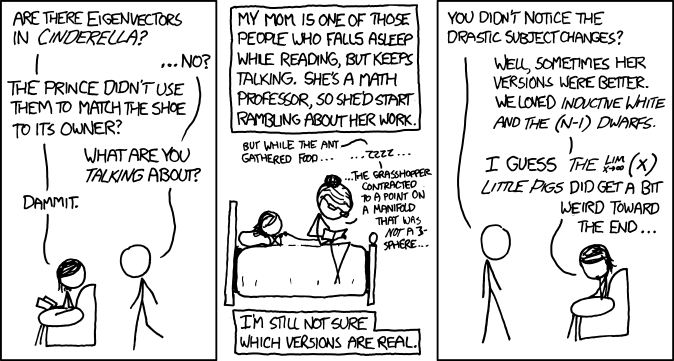
\includegraphics[width=.55\textwidth]{Dateien/00xkcd.png}\\
    Erzählt uns, wenn es euch auch so geht. Wir kennen da einen guten Arzt.\\
    Bildquelle: \url{https://xkcd.com/872/}
\end{figure}
\vfill
Moin, dies sind die informellen Notizen begleitend zu unserem MfP2-Tutorium.\\
Diese sind primär als unsere eigene Vorbereitung auf die Tutorien zu sehen, ihr könnt sie aber gerne nutzen, um euer Wissen zur Vorlesung zu vertiefen.\\
Hier greifen wir einige der wichtigsten Sätze und Definitionen auf, um diese dann durch Beispiele zu veranschaulichen. Lasst euch nicht davon abschrecken, dass wir manchmal noch ein bisschen mehr dazu schreiben - Wir empfehlen sogar eher, dies als Nachschlagewerk zu nutzen, das \Skript{} ersetzt es auf keinen Fall!\\
Wichtig ist auch: Viele Satzbezeichnungen und die Nummerierung der Definitionen, Sätze und Beispiele sind nur \red{inoffiziell} und dienen der internen Übersicht in diesen Notizen, ihr solltet also bei der Bearbeitung eurer Übungsaufgaben nicht darauf verweisen (nehmt stattdessen lieber die Folien im Skript).\\
Viele weitere Aufgaben zur Klausurvorbereitung findet ihr in unserer Aufgabensammlung.\\
Bei Anmerkungen oder Fragen (es haben sich bestimmt noch einige Fehler eingeschlichen) schreibt uns einfach bei Telegram oder schickt uns eine E-Mail an fabian.balzer@studium.uni-hamburg.de.\\\\
Viel Erfolg beim Lernen und Üben!\\
:)
\cfoot{\pagemark}



\ifnum\value{reduce_to_selection}=0 {
    \tableofcontents
}\fi


%%%%%%%%%%%%%%%%%%%%%%%%%%%%%%%%%%%%%%%%%%%%%%%%%%%%%%%%%%%%%%%%%
\newpage
\section[Vektorräume (Wdh. Mathe 1)]{Vektorräume, Unterräume und ein Haufen Definitionen (Basen, lineare Unabhängigkeit, Erzeugnis)}
\Einleitung{\red{Achtung, die ersten Kapitel sind eine Aufarbeitung der Themen aus Mathe 1.}
Wir wenden uns zu Beginn einer wichtigen mathematischen Struktur, den Vektorräumen, zu.\\
Viele Objekte, die wir aus der Physik kennen - z. B. Kräfte oder Wellen - zeigen ein Verhalten, das genau dieser Struktur entspricht. Um ordentlich damit umgehen zu können, definieren wir uns ein Netz an Begriffen, um Vektoren und Relationen zwischen Vektoren näher zu klassifizieren.\\
Gerade im Hinblick auf das zweite (und alle weiteren) Semester ist es enorm wichtig, dass ihr diese Begriffe möglichst schnell verinnerlicht.}
\subsection{Vektorräume}\label{ssec:Vektorraum}
Wenn euch von nun an jemand fragt, was ein Vektorraum ist, sollte euch die Definition sofort einfallen:
\begin{Def}
{Vektorraum}
Ein \red{Vektorraum über $\mathbb{K}$}\footnote{$\mathbb{K}$ ist einfach der Körper (wie z. B. $\mathbb{R}$), aus dem die Skalare für die Multiplikation kommen.} ist eine \underline{Menge} $V$ zusammen mit der \red{vektoriellen Addition} und der \red{skalaren Multiplikation} bzgl. von $\mathbb{K}$.\\
\begin{tabular}{l|l|l}
    \textbf{Name} &\textbf{ Definition }&\textbf{ Erklärung} \\
    \hline
    Addition: & $V\times V\to V:\, (v,w)\mapsto v+w$ &\parbox[t]{5cm}{\blue{Die Summe zweier Vektoren ist wieder ein Vektor.}} \\
    Skalare Multiplikation: & $\mathbb{K}\times V\to V:\,(\lambda, v)\mapsto \lambda \cdot v$ & \parbox[t]{5cm}{\blue{Wir können Vektoren skalieren und erhalten dadurch wieder Vektoren.}}
\end{tabular}
Wie wir später sehen werden, nennt man die Kombination aus Addition und Multiplikation verschiedener Vektoren \red{Linearkombination}.
\end{Def}
Addition und Multiplikation müssen dabei bestimmte Eigenschaften erfüllen, damit wir wie gewohnt rechnen können:\\
$(V,+)$ muss eine \underline{kommutative Gruppe} sein.
\begin{Def}
{Kommutative Gruppe}
Für eine kommutative Gruppe $(V,+)$ gelten die folgenden Relationen für alle $v,w,u\in V$:
\begin{enumerate}
    \item \textbf{Kommutativgesetz}:\\
    $v+w=w+v$
    \item \textbf{Assoziativgesetz}:\\
    (u+v)+w=u+(v+w)
    \item \textbf{Nullelement}:\\
    Es existiert $0\in V$, sodass $v+0=v$ gilt.
    \item \textbf{Additives Inverses}:\\
    Für alle $v$ existiert $-v$, sodass $v+(-v)=0$.
\end{enumerate}
Nullelement und additive Inverse sind eindeutig.
\end{Def}
Die skalare Multiplikation muss hingegen folgende Relationen\footnote{Die ihr als Assoziativgesetz, Neutrales Element und Distributivgesetze kennt} erfüllen:
\begin{align*}
    (\lambda\mu)\cdot v&=\lambda(\mu\cdot v)\\
    1\cdot v&= v\\
    (\lambda+\mu)\cdot v&=\lambda \cdot v+\mu \cdot v\\
    \lambda\cdot(v+w)&=\lambda \cdot v+\lambda \cdot w.
\end{align*}
\begin{Beispiel}
{Funktionen bilden einen Vektorraum (2/2)}
Wir können Funktionen $f\in \Abb(X,\mathbb{K})$\footnote{Mit $\Abb(X,\mathbb{K})$ meinen wir Abbildungen von der Menge $X$ in den Körper $\mathbb{K}$.} als Vektoren auffassen bzw. $\Abb(X,\mathbb{K})$ als Vektorraum über $\mathbb{K}$:
\begin{eqnarray*}
+:&&\Abb(X,\mathbb{K})\times \Abb(X,\mathbb{K})\to \Abb(X,\mathbb{K}):\,(f+g)(x)=f(x)+g(x)\quad (x\in X)\\
\cdot:&&\mathbb{K}\times \Abb(X,\mathbb{K})\to \Abb(X,\mathbb{K}):\,(\lambda f)(x)=\lambda\cdot f(x)\quad (\lambda\in\mathbb{K}).
\end{eqnarray*}
\end{Beispiel}
\begin{Beispiel}{Ein kartesischer Raum (2/2)}
Der $\mathbb{R}^3=\{(x,y,z)\furdas x,y,z\in\mathbb{R}\}$ als Spezialfall des kartesischen Raumes (Folie 319 im Mathe-1-Skript) ist mit
\begin{eqnarray*}
+:&&\mathbb{R}^3\times\mathbb{R}^3\to\mathbb{R}^3, \Matrix{x\\y\\z}+\Matrix{a\\b\\c}=\Matrix{x+a\\y+b\\z+c}\text{ und }\\
\cdot:&&\mathbb{R}\times\mathbb{R}^3\to\mathbb{R}^3,\,\lambda\Matrix{x\\y\\z}=\Matrix{\lambda x\\\lambda y\\\lambda z}
\end{eqnarray*}
ein Vektorraum.\\
Als Notation für Vektoren $v\in\mathbb{R}^3$ nutzen wir in diesen Notizen Spaltenvektoren.
\end{Beispiel}
\subsubsection{Untervektorräume}
Für viele Anwendungen benötigen wir nur Teilmengen eines Vektorraums $V$ (anschaulich z. B. eine Ebene im $\mathbb{R}^3$).\\
Diese Teilmenge $U$ erbt automatisch die Addition (A) und Multiplikation (M) des Vektorraumes, jedoch wird zusätzlich die \underline{Abgeschlossenheit} gefordert, d. h. dass wir durch (A) und (M) (also Linearkombinationen von Vektoren aus $U$) nicht plötzlich außerhalb von $U$ landen dürfen.\\
Zudem interessieren uns leere Mengen nicht wirklich, weshalb diese per Definition keine Untervektorräume sind.
\begin{Def}
{Untervektorräume}
Ein \red{Unterraum}\footnote{oder \red{Untervektorraum}} $U$ eines Vektorraumes $V$ über $\mathbb{K}$ muss also folgende Eigenschaften erfüllen:
\begin{enumerate}
    \item \textbf{Teilmenge}:\\
    $U\subseteq V$, \blue{$U$ ist eine Teilmenge von $V$.}
    \item \textbf{Nicht leer}:\footnote{Da freue ich mich bei meinem Kühlschrank auch immer.}\\
    $U\neq\emptyset$, \blue{$U$ ist nicht die leere Menge.}
    \item \textbf{Additive Abgeschlossenheit}:\\
    $v+w\in U\,\forall v,w\in U$, \blue{$U$ ist abgeschlossen bzgl. der vektoriellen Addition.}
    \item \textbf{Multiplikative Abgeschlossenheit}:\\
    $\lambda \cdot v\in U\,\forall \lambda\in\mathbb{K}, v\in U$, \blue{$U$ ist abgeschlossen bzgl. der skalaren Multiplikation.}
\end{enumerate}
\end{Def}

\begin{Satz}
{Vorgehensweise}{Untervektorraum zeigen/Widerlegen}
Wenn ihr also zeigen wollt, dass etwas ein Unterraum ist, müsst ihr für 2) irgendein Element finden - am einfachsten ist häufig der Nullvektor - und anschließend 3) und 4) allgemein zeigen.\\
Zum Widerlegen nutzt ihr einfach 3) oder 4) mit konkreten Elementen.
\end{Satz}
\begin{Beispiel}
{Polynome bilden einen Untervektorraum (1/4)}
\Zz{Polynome von Grad ${\leq n}$ mit Koeffizienten aus $\mathbb{K}$ (im folgenden bezeichnet als $\mathbb{K}[x]_{\leq n}$) der Form
\begin{equation*}
    P:\mathbb{K}\to\mathbb{K},\,x\mapsto P(x)=a_0+a_1x+a_2x^2+...=\sum_{k=0}^na_kx^k
\end{equation*}
bilden einen Untervektorraum der Funktionen von $\mathbb{K}\to\mathbb{K}$ ($\Abb(\mathbb{K},\mathbb{K}$).}
\Zb{(Auch wenn das natürlich kein vollständiger Beweis ist, betrachten wir $\mathbb{K}=\mathbb{R}$, also $\mathbb{R}[x]_{\leq n}\subseteq\Abb(\mathbb{R},\mathbb{R})$.)
\begin{enumerate}\setcounter{enumi}{1}
    \item $\mathbb{R}[x]_{\leq n}$ ist nicht leer, denn $P:\mathbb{R}\to\mathbb{R},\, P(x)=0$ ist ein Polynom ($P\in\mathbb{R}[x]_{\leq n}$).
    \item Seien $P(x):=\sum_{k=0}^na_kx^k$ und $Q(x):=\sum_{k=0}^nb_kx^k\in\mathbb{R}[x]_{\leq n}$. Dann ist
    \begin{equation*}
        P(x)+Q(x)=\sum_{k=0}^na_kx^k+\sum_{k=0}^nb_kx^k=\sum_{k=0}^n(a_k+b_k)x^k=:\sum_{k=0}^nc_kx^k\in \mathbb{R}[x]_{\leq n}.\,\checkmark
    \end{equation*}
    \item Sei zudem $\lambda\in\mathbb{R}$, so gilt
    \begin{equation*}
        \lambda\cdot P(x)=\lambda\sum_{k=0}^na_kx^k=\sum_{k=0}^n\lambda a_kx^k=:\sum_{k=0}^nd_kx^k\in \mathbb{R}[x]_{\leq n}.\,\checkmark
    \end{equation*}
\end{enumerate}}\\
Anmerkung: Nur die Polynome von Grad $n$ (d. h. Polynome der Form $f(x)=\sum_{k=0}^na_kx^k$ mit $a_n\neq0$) bilden KEINEN Untervektorraum, da durch Linearkombination zweier solcher Polynome die Nullfunktion erzeugt werden kann (z. B. $g(x)=f(x)-f(x)=0$ \Lightning), die ja kein Polynom von Grad $n$ mehr ist.
\end{Beispiel}
\begin{Beispiel}
{Die Gerade als Unterraum mit einem Vektor (2/4)}
\begin{tabular}{c l}
\parbox[b]{10cm}{
\Zz{Die Gerade $\mathbb{R}v=\{\mu v\furdas\mu\in\mathbb{R}\}\subseteq\mathbb{R}^2$ ist $\forall v\in\mathbb{R}^2$ der kleinste Unterraum, der $v$ enthält.}
} & 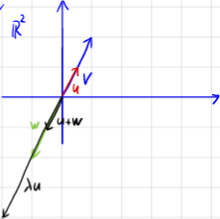
\includegraphics[width=.2\textwidth]{Dateien/00/11GeradeUnterraum.PNG}
\end{tabular}\\
\Zb{Wir zeigen, dass es ein Unterraum ist:\\
Fallunterscheidung: Sei $v=\Vec{0}$, so ist $\mathbb{R}v=\{0\}\subseteq \mathbb{R}^2$ offensichtlich ein Unterraum, der die Eigenschaften erfüllt.\\
Für $v\neq0$: Es seien $u, v\in\mathbb{R}v$ und $\lambda\in\mathbb{R}$
\begin{enumerate}\setcounter{enumi}{1}
    \item $v=1\cdot v$ ist ein Element aus $\mathbb{R}v$, d. h. $\mathbb{R}v$ ist nicht leer.
    \item Es gilt $u+v=\mu_1 v+\mu_2 v=(\mu_1+\mu_2)v=:s\in\mathbb{R}v.\,\checkmark$
    \item Es gilt $\lambda u=\lambda\mu_1 v=(\lambda\mu_1)v=:t\in\mathbb{R}v.\,\checkmark$
\end{enumerate}}
\end{Beispiel}
\begin{Beispiel}
{Affine Geraden sind keine Unterräume (3/4)}
\begin{tabular}{c l}
\parbox[b]{8cm}{
Die \red{affinen Geraden} $G_a:=\{v\in\mathbb{R}^2\furdas v=\mu u+w,\mu\in\mathbb{R}\}$ mit festen Richtungs- und Stützvektoren $u,w\in\mathbb{R}^2\{\Vec{0}\}$ bilden keinen Unterraum des $\mathbb{R}^2$, denn\\
für $x,y\in G_a,$ also $x=\mu_1u+w$, $y=\mu_2+w$ ist\\
$x+y=(\mu_1+\mu_2)u+2w\neq \mu_3 u+w$.\\
Zudem ist $\lambda x=\mu_1\lambda u+ \lambda w=v+(\mu-1)w\notin G_a$ für $\lambda\neq1$, wobei $v:= \lambda \mu_1 u+w\in G_a$ ist.
} & 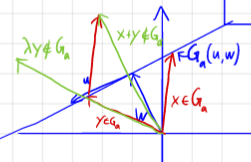
\includegraphics[width=.4\textwidth]{Dateien/00/11KeinUnterraum.PNG}
\end{tabular}
\end{Beispiel}
\begin{Beispiel}
{Ein weiterer Unterraum? (4/4)}
Ist $U:=\{\Matrix{x\\y\\z}\in\mathbb{R}^3\furdas z=x y, \,x,y\in\mathbb{R}\}$ ein Unterraum des $\mathbb{R}^3$?\\
Nein, denn $U$ ist nicht abgeschlossen bezüglich der Addition:\\
Seien $v:=\Matrix{1\\0\\0}$ und $w:=\Matrix{0\\1\\0}$ Vektoren aus $U$.\\
Die Summe $v+w=\Matrix{1\\1\\0}$ ist nicht aus $U$, da die dritte Komponente nicht mehr das Produkt aus den ersten beiden ist.\\
Ist $U$ abgeschlossen bezüglich der skalaren Multiplikation?
\end{Beispiel}
\begin{Def}
{Bezeichnungen verschiedener Funktionenräume}
Wir definieren für ein Intervall $I\subset \mathbb{R}$ verschiedene Klassen von Funktionen:\\
\begin{tabular}{l|l|l}
    \textbf{Bezeichnung} &\textbf{ Bedeutung }&\textbf{ Erklärung} \\
    \hline
    $\Abb(I,\mathbb{R})$ & $\{f:I\to\mathbb{R}\}$ & \parbox[t]{5.4cm}{Jegliche Funktionen von $I$ nach $\mathbb{R}$}\\
    $C(I,\mathbb{R})$ & $\{f:I\to\mathbb{R}\furdas f \text{ stetig}\}$ & \parbox[t]{5.4cm}{Stetige Funktionen von $I$ nach $\mathbb{R}$}\\
    $\Diff(I,\mathbb{R})$ & $\{f:I\to\mathbb{R}\furdas f \text{ diffbar}\}$ & \parbox[t]{5.4cm}{Differenzierbare Funktionen von $I$ nach $\mathbb{R}$}\\
    $C^k(I,\mathbb{R})$ & $\{f:I\to\mathbb{R}\furdas f\, k \text{-fach stetig diffbar}\}$ & \parbox[t]{5.4cm}{$k$-fach stetig differenzierbare\footnote{Das heißt, dass die $k$-te Ableitung stetig ist.} Funktionen von $I$ nach $\mathbb{R}$}
\end{tabular}
Jetzt wisst ihr also, was gemeint ist, wenn von $C^\infty$-Funktionen gesprochen wird.
\end{Def}
\begin{Satz}
{Satz}{Unterrauminklusion für Funktionenräume}
Für $1\leq k\in\mathbb{N}$ gilt die folgende Unterrauminklusion:
\begin{equation*}
    \mathbb{R}[x]_{\leq n}\subseteq C^\infty(I,\mathbb{R})\subseteq C^k(I,\mathbb{R})\subseteq\Diff(I,\mathbb{R})\subseteq C(I,\mathbb{R})\subseteq\Abb(I,\mathbb{R}).
\end{equation*}
Die Polynome sind also ein Unterraum der unendlich oft stetig differenzierbaren Funktionen, welche ein Unterraum der $k$-fach stetig differenzierbaren Funktionen sind, welche ein Unterraum der differenzierbaren Funktionen sind, welche ein Unterraum der stetigen Funktionen sind, welche wiederum ein Unterraum der Funktionen sind. Puh.
\end{Satz}

\subsubsection{Vokabelbombardement}
Es folgt nun eine Reihe von Definitionen, die alle eng miteinander verknüpft sind, also gut aufpassen! Die Beispiele sollen euch helfen, wenn ihr nicht direkt seht, was mit den Definitionen gemeint ist, ihr könnt sie aber auch erstmal überspringen, um euch einen Überblick zu verschaffen.\\
Im Folgenden sei $V$ stets ein Vektorraum über einem Körper $\mathbb{K}$ (z. B. über $\mathbb{R}$).
\begin{Def}
{Familien von Vektoren}
Eine \red{Familie}\footnote{Die Begriffe der Mathematiker sind z.T. direkt aus dem Leben gegriffen. Falls ihr irgendwann vorhabt, Topologie zu hören, wird euch vielleicht das \textit{Geschlecht} von Flächen über den Weg laufen, genauso wie man in der Funktionentheorie Funktionen ein Geschlecht zuweist. Auch die Begrifflichkeit \textit{fast alle} ist tatsächlich streng mathematisch definiert.} ist schlicht eine indizierte\footnote{jedem Element wird ein Index zugewiesen} Menge, z. B. $(v_i)_{i\in J}$ mit den Vektoren $v_i\in V$ und einer Indexmenge $J$.\\
Indexmengen dürfen bei Familien auch überabzählbar sein.
\end{Def}
Einen Spezialfall hatten wir mit den Folgen kennengelernt (z. B. $(a_n)_{n\in\mathbb{N}}$, $a_n\in\mathbb{R}$).\\
Hier waren die Elemente der Familie die reellen Zahlen $a_n$, die Indexmenge war $\mathbb{N}$.
\begin{Beispiel}
{Musterfamilie (1/2)}
Ein Beispiel aus $\mathbb{R}^3$ wäre die Familie $(v_i)_{i\in\{1,2,5\}}$ mit 
\begin{equation*}
    v_1:=\Matrix{1\\2\\3},\quad v_2:=\Matrix{1\\0\\0},\quad v_5:=\Matrix{2\\1\\0},
\end{equation*}
d. h. im Prinzip die Menge $\left\{\Matrix{1\\2\\3},\Matrix{1\\0\\0},\Matrix{2\\1\\0}\right\}$ mit indizierten Elementen.
\end{Beispiel}
\begin{Beispiel}
{Reelle Familie (2/2)}
Andererseits ist auch eine Familie mit reellem Index $a$ möglich:
\begin{equation*}
    (v_a)_{a\in\mathbb{R}}:=\BracedIn{\Matrix{a\\a^2\\-5a}}_{a\in\mathbb{R}}.
\end{equation*}
\end{Beispiel}
\begin{Def}
{Linearkombination}
Wenn wir einen Vektor $v\in V$ durch eine \underline{endliche} Familie von Vektoren $(v_i)_{i\in J}$, also $v_i=v_1,...,v_r$ mit Koeffizienten $\lambda_i$ aus $\mathbb{K}$ durch
\begin{equation*}
    \boxed{v=\sum_{i=1}^r\lambda_i v_i}
\end{equation*}
darstellen können, so nennen wir $v$ eine \red{Linearkombination} der Vektoren $(v_i)_{i\in J}$.
\end{Def}
\begin{Beispiel}[label=beisp:LinKombVektoren]
{Was ist möglich{,} was nicht?}
Wir betrachten die Vektoren
\begin{equation*}
    \boxed{v_1:=\Matrix{1\\2\\3},\quad v_2:=\Matrix{1\\1\\2},\quad v_3:=\Matrix{-1\\0\\-1},\quad v_4:=\Matrix{1\\4\\5}}.
\end{equation*}
$v_1$ kann als Linearkombination von $v_2$ und $v_3$ ausgedrückt werden, denn\\
$v_1=2v_2+v_3$.\\
$v_4$ kann nicht durch $v_1$ und $v_2$ dargestellt werden, denn das Gleichungssystem\\
$\lambda_1 v_1+\lambda_2 v_2=v_4$ ist nicht lösbar, wir wir hier sehen:
\begin{equation*}
    \Matrix{\lambda_1+\lambda_2\\2\lambda_1+\lambda_2\\3\lambda_2+2\lambda_2}=\Matrix{1\\4\\5}
\end{equation*}
Die erste Gleichung besagt $\lambda_1=1-\lambda_2$, woraus mit der zweiten\\$2\lambda_1+\lambda_2=4\Leftrightarrow 2-\lambda_2=4\Leftrightarrow\boxed{\lambda_2=2},\,\boxed{\lambda_1=-1}$ folgt.\\
Eingesetzt in die dritte ergibt dies aber $3\cdot2+2\cdot(-1)=5$. \Lightning
\end{Beispiel}
\begin{Def}
{Lineare Hülle}
Die Menge aller Vektoren aus $V$, die durch Linearkombination aus den Vektoren einer Familie $(v_i)_{i\in J}$ dargestellt werden können, nennt man \red{lineare Hülle}.\footnote{oder manchmal auch \red{lineares Erzeugnis}}\\
\textbf{Notation}:\\
$\Span{v_i}{i\in J}=\{v\furdas v\text{ ist Linearkombination der Familie } (v_i)_{i\in J}\}$.
\end{Def}
Anschaulich kann man sich dies vorstellen als der Unterraum, der durch die Vektoren der Familie aufgespannt wird - daher auch der Name.
\begin{Beispiel}{Vektoren aus der linearen Hülle}
Bezogen auf die Vektoren aus Beisp. \ref{beisp:LinKombVektoren} und unsere Feststellungen dort ist also
\begin{equation*}
    v_1\in\Spann{v_2,v_3}\text{ und }v_4\notin\Spann{v_1,v_2}
\end{equation*}
\end{Beispiel}
\begin{Def}
{Lineare Unabhängigkeit}
Eine besondere Bedeutung hat die Darstellung des Nullvektors als Linearkombination:\\
Wir nennen die Familie $(v_i)_{i\in J}$ \red{linear unabhängig}, wenn der Nullvektor nur durch Linearkombination der $(v_i)_{i\in J}$ dargestellt werden kann, wenn \underline{alle} Koeffizienten $\lambda_i=0$ sind, d. h.
\begin{equation*}
    \Vec{0}=\sum_{i=1}^r\lambda_iv_i\Rightarrow \lambda_i=0\,\forall i.
\end{equation*}
\end{Def}
Anders gesagt: Man kann keinen der Vektoren aus der Familie durch Linearkombination der anderen darstellen.
\begin{Beispiel}
{Vektoren des $\mathbb{R}^3$ (1/2)}
Sind die Vektoren $v_1$ und $v_2$ aus Beisp. \ref{beisp:LinKombVektoren} linear unabhängig?\\
Starte mit $\lambda_1v_1+\lambda_2v_2=0$, $\lambda_1, \lambda_2\in\mathbb{R}$.\\
Dann besagen die beiden ersten Zeilen der Gleichung
\begin{eqnarray*}
    (I)&&\,\lambda_1+\lambda_2=0\Rightarrow\lambda_1=-\lambda_2\\
    (II)&&\,2\lambda_1+\lambda_2=0\overset{(I)}{\Rightarrow}1(-\lambda_2)+\lambda_2=0\Rightarrow\lambda_2=0\Rightarrow\lambda_1=0
\end{eqnarray*}
Also sind $v_1$ und $v_2$ linear unabhängig.\\
Tatsächlich ist die Familie $(v_i)_{i\in\{1,2,3\}}$ linear abhängig und die Familie $(v_i)_{i\in\{1,2,4\}}$ linear unabhängig.
\end{Beispiel}
\begin{Beispiel}
{Monome (2/2)}
\Zz{Die Monome $(1,x,x^2,x^3,...,x^n)$ sind linear unabhängig im Vektorraum der Polynome $\mathbb{R}[x]{\leq n}$ von Grad $\leq n$.}
\Zb{Der Trick hier ist, dass die Gleichung $\sum_{k=0}^n\lambda_kx^k=0$ für alle $x\in\mathbb{R}$ erfüllt sein muss, also auch für $x=0$.\\
Für $x=0$ folgt sofort: $\lambda_0+\lambda_1\cdot0+0+...=0\Rightarrow\lambda_0\overset{!}{=}0$.\\
Der nächste Trick ist nun, einfach auf beiden Seiten der Gleichung abzuleiten, denn dann muss die Gleichung immer noch für alle $x\in\mathbb{R}$ erfüllt sein. Abgeleitet haben wir:
\begin{equation*}
    \sum_{k=1}^nk\lambda_kx^{k-1}=0\Leftrightarrow\sum_{k=0}^n(k+1)\lambda_{k+1}x^k=0\overset{x=0}{\Rightarrow}\lambda_1+2\lambda_2\cdot0+...=0\Rightarrow \lambda_1=0.
\end{equation*}
Wir argumentieren also wieder mit $x=0$.\\
Führen wir dies $n$ mal durch, erhalten wir $\lambda_i=0$ für alle $i\in\{0,1,...,n\}$.}
\end{Beispiel}
Die lineare Unabhängigkeit von Vektoren liefert uns eine schöne Eigenschaft:
\begin{Satz}
{Satz}{Eindeutigkeit der Darstellung durch linear unabhängige Familie}
Jeder Vektor $v$, der durch Linearkombination aus Vektoren einer linear unabhängigen Familie $(v_i)_{i\in J}$ dargestellt werden kann, d. h. $v\in\Span{v_i}{i\in J}$, besitzt eine \underline{eindeutige} Darstellung,
\begin{equation*}
    v=\sum_{i=1}^r\lambda_iv_i.
\end{equation*}
\end{Satz}
\begin{Def}
{Erzeugendensystem}
Wir nennen eine Familie $(v_i)_{i\in J}\in V$ ein \red{Erzeugendensystem}, wenn wir \underline{alle} Vektoren aus $V$ durch Linearkombination durch die $v_i$ darstellen können, d. h. $\Span{v_i}{i\in J}=V$.
\end{Def}
\begin{Def}
{Basis}
Ist ein Erzeugendensystem zudem linear unabhängig, so nennen wir es eine \red{Basis} von $V$.\\
Zusammen mit dem Satz über Eindeutigkeit hat also jeder Vektor $v\in V$ eine eindeutige Darstellung bezüglich einer Basis.
\end{Def}
\begin{Beispiel}
{Kanonische Basis (1/2)}
Die kanonische Basis des $\mathbb{R}^n$ ist $(e_1,e_2,...,e_n)$ mit $e_i:=(0,0,...,1,0,...)$.\footnote{mit der 1 an der $i$-ten Stelle}\\
Der Vektor $v=\Matrix{1\\-3.5}$ hab bzgl. der Standardbasis des $\mathbb{R}^2$ die Darstellung\\$v=1e_1-3.5e_2$.\\
Bezüglich einer anderen Basis wie z. B. $(b_1,b_2):=(e_1+e_2,e_1)$ ist die Darstellung jedoch\\
$v=-3.5b_1+2.5b_2$.
\end{Beispiel}
\begin{Beispiel}
{Monome als Basis (2/2)}
Die Monome $(1,x,x^2,...)$ bilden eine Basis der Polynome $\mathbb{R}[x]$.
\end{Beispiel}
\subsubsection{Aussagen über Basen}
Die folgenden Aussagen sind enorm wichtig für das Verständnis und sollten irgendwann auch intuitiv Sinn ergeben!
\begin{Satz}
{Satz}{Charakterisierung der Basis}
Eine Basis eines Vektorraumes $V$...
\begin{enumerate}
    \item ...ist stets ein \underline{minimales Erzeugendensystem}, d. h. jedes Erzeugendensystem von $V$ hat mindestens so viele Komponenten wie eine Basis.
    \item ...ist eine \underline{maximal linear unabhängige Familie}, d. h. es lässt sich kein weiterer Vektor hinzufügen, sodass die Familie linear unabhängig bleibt.
    \item Wie schon erwähnt: Jeder Vektor aus $V$ besitzt eine \underline{eindeutige} Darstellung bzgl. einer Basis.
    \item Jedes endliche Erzeugendensystem von $V$ enthält eine Basis (\red{Basisauswahlsatz}).
    \item Wenn $V$ eine endliche Basis besitzt,\footnote{d. h. die Basis besteht aus endlich vielen Vektoren} so ist jede Basis endlich und hat die \underline{gleiche Anzahl} an Elementen.
\end{enumerate}
\end{Satz}
\begin{Satz}
{Lemma}{Austauschlemma}
Wir dürfen den $k$-ten Basisvektor einer gegebenen Basis $(v_i)_{i\in J}\in V$ durch eine beliebige Linearkombination $w=\sum_{i=1}^n\lambda_iv_i$ austauschen, d. h. $(v_1,...,v_{k-1},w,v_{k+1},...)$ ist auch eine Basis, wenn $\lambda_k\neq 0$, wenn also $w$ einen endlichen Anteil von $v_k$ enthält.
\end{Satz}
\begin{Satz}
{Satz}{Steinitzscher Austauschsatz}
Wir können jede linear unabhängige Familie $(w_1,...,w_r)$ mithilfe einer Basis $(v_1,...,v_n)$ zu einer Basis von $V$ ergänzen.
\end{Satz}
\subsubsection{Dimension}
Vektorräume mit endlich vielen Basisvektoren können wir nun eindeutig über die Anzahl der Basisvektoren charakterisieren.
\begin{Def}
{Dimension}
Hat $V$ eine endliche Basis mit $n$ Elementen, so nennen wir diese Zahl die \red{Dimension} $\dim V=n$ von $V$.\\
Ist $V=\{\Vec{0}\}$, so ist $\dim V=0$. Andererseits ist $\dim V=\infty$.
\end{Def}
\begin{figure}[htbp]
\centering
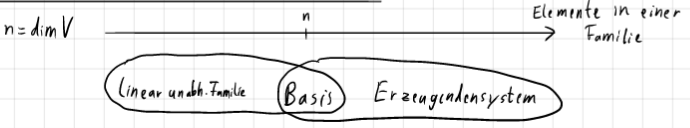
\includegraphics[width=.7\textwidth]{Dateien/00/11Dimensionschaubild.PNG}
\caption*{Veranschaulichung der Zusammenhänge zwischen linear unabhängiger Familie, Basis, Erzeugendensystem und Dimension.}
\end{figure}
\begin{Satz}
{Folgerung}{Zusammenfassung der Erkenntnisse}
Sei $V$ ein Vektorraum mit $\dim V= n$ und $(v_i)_{i\in J}$ eine Familie von Vektoren.
\begin{enumerate}
    \item Ist $(v_i)_{i\in J}$ \underline{linear unabhängig}, so hat sie \underline{höchstens} $n$ Elemente.
    \item Ist $(v_i)_{i\in J}$ \underline{linear unabhängig}, so ist sie genau dann eine Basis, wenn sie $n$ Elemente hat.
    \item Ist $(v_i)_{i\in J}$ ein \underline{Erzeugendensystem}, so hat sie \underline{mindestens} $n$ Elemente.
    \item Ist $(v_i)_{i\in J}$ ein \underline{Erzeugendensystem}, so ist sie genau dann eine Basis, wenn sie $n$ Elemente hat.
\end{enumerate}
\end{Satz}
\blue{Das waren jetzt sehr viele Definitionen und Sätze, die sich gegenseitig ergänzen. Nehmt euch auf jeden Fall die Zeit, alle Zusammenhänge zu verstehen!}
\subsection{Gaußscher Algorithmus}
\blue{Wir gucken uns nun einen sehr nützlichen Algorithmus an, um Basen eines Vektorraums aus einem Erzeugendensystem zu bestimmen.\\
Dieser hilft zudem bei der Überprüfung linearer Unabhängigkeit und beim Lösen linearer Gleichungssysteme.}
\begin{Satz}
{Merksatz}{Gaußscher Algorithmus}
Wir gehen bei einem Gleichungssystem oder bei gegebenen Vektoren, bei denen fraglich ist, ob sie eine Basis bilden, folgendermaßen vor (falls etwas unklar ist, siehe die folgenden Beispiele):
\begin{enumerate}
    \item Schreibe die Vektoren oder Koeffizienten als Matrix.
    \item
\begin{tabular}{c l}
\parbox[b]{9.5cm}{
Wende die folgenden erlaubten Umformungen an, um die Matrix auf \textit{Zeilenstufenform} zu bringen:
} & 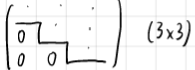
\includegraphics[width=.25\textwidth]{Dateien/00/11Zeilenstufenform.PNG}
\end{tabular} 
    \begin{enumerate}
        \item Vertauschen zweier Zeilen.
        \item Multiplizieren von Zeilen mit Skalaren $\lambda\in\mathbb{K}\setminus\{0\}$.
        \item Addieren von Vielfachen einer Zeile zu anderen Zeilen.
    \end{enumerate}
    \item Bei Gleichungungssystemen: Zurückführen auf die Gleichungen und diese von unten ausgehend zeilenweise abarbeiten.\\
    Beim Finden der Basis: Einfach die Nicht-Null-Zeilen ablesen.
\end{enumerate}
\end{Satz}
\begin{Beispiel}
{Lösen eines Gleichungssystems (1/4)}
Zu lösen seien die Gleichungen
\begin{align*}
    2x+3y+4z&=10\quad (I)\\
    6y-2z&=5\quad (II)\\
    -8x+z&=12\quad (III).
\end{align*}
\begin{enumerate}
    \item Wir schreiben die Koeffizienten als Matrix:
\begin{center}
    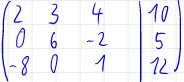
\includegraphics[width=.2\textwidth]{Dateien/00/11GaussA1.PNG}
\end{center}
    \item Wir wenden die erlaubten Umformungen an:
\begin{center}
    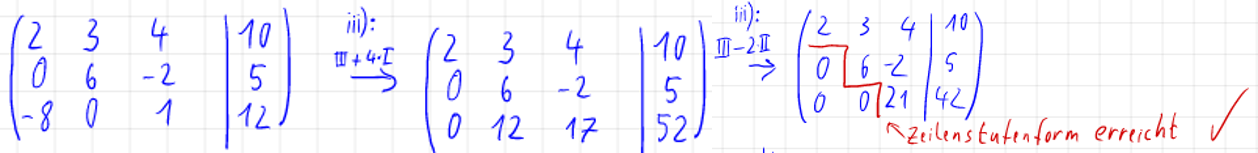
\includegraphics[width=.7\textwidth]{Dateien/00/11GaussA2.PNG}
\end{center}
    \item Wir führen dies auf die Gleichungen zurück und arbeiten uns von unten nach oben durch:
\begin{center}
    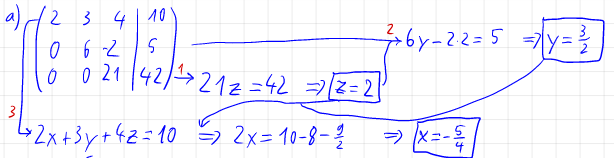
\includegraphics[width=.6\textwidth]{Dateien/00/11GaussA3.PNG}
\end{center}
\end{enumerate}
\begin{equation*}
    \Matrix{x\\y\\z}=\Matrix{-5/4\\3/2\\2}
\end{equation*}
löst also das Gleichungssystem.\\
\blue{\textbf{Anmerkung}:\\
Wir werden bald sehen, dass wir das Gleichungssystem auch so aufschreiben können:
\begin{center}
    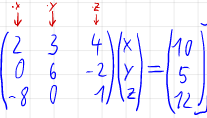
\includegraphics[width=.2\textwidth]{Dateien/00/11GaussA4.PNG}
\end{center}
}
\end{Beispiel}
\begin{Beispiel}
{Finden einer Basis (2/4)}
Wir suchen eine Basis des Unterraumes $U:=\Span{v_i}{i\in\{1,2,3\}}\subseteq\mathbb{R}^4$ mit den Vektoren
\begin{equation*}
    v_1=\Matrix{-2\\-2\\-5\\6},\quad v_2=\Matrix{1\\1\\2\\-2},\quad v_3=\Matrix{4\\4\\10\\-12}.
\end{equation*}
\begin{enumerate}
    \item Wir schreiben die Vektoren als Zeilen in eine Matrix:
\begin{center}
    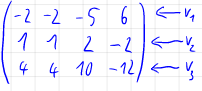
\includegraphics[width=.2\textwidth]{Dateien/00/11GaussB1.PNG}
\end{center}
    \item Wir wenden die erlaubten Umformungen an:
\begin{center}
    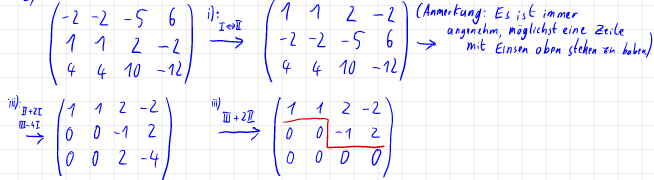
\includegraphics[width=.7\textwidth]{Dateien/00/11GaussB2.PNG}
\end{center}
    \item Wir führen dies auf Basisvektoren zurück
\begin{center}
    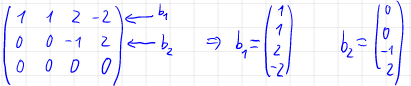
\includegraphics[width=.6\textwidth]{Dateien/00/11GaussB3.PNG}
\end{center}
\end{enumerate}
$U$ ist also ein zweidimensionaler Untervektorraum des $\mathbb{R}^4$.\\
\blue{\textbf{Anmerkung}:\\
Zwar ist diese Basis nicht eindeutig, aber die Anzahl der Basisvektoren ist durch die Dimension des Unterraums festgelegt.}
\end{Beispiel}
\begin{Beispiel}
{Lineare Unabhängigkeit und Basis prüfen (3/4)}
Bilden die folgenden Vektoren eine Basis des $\mathbb{R}^3$?
\begin{equation*}
    v_1=\Matrix{0\\1\\2},\quad v_2=\Matrix{2\\1\\0},\quad v_3=\Matrix{1\\0\\2}
\end{equation*}
Wenn sie linear unabhängig sind, ist das der Fall (da $\dim \mathbb{R}^3=3=\#v_i$).\\
Wir prüfen also, ob das lineare Gleichungssystem $\lambda_1v_1+\lambda_2v_2+\lambda_3v_3=\Vec{0}$ nur durch $\lambda_1=\lambda_2=\lambda_3=0$ zu lösen ist. Das können wir folgendermaßen aufschreiben:
\begin{center}
    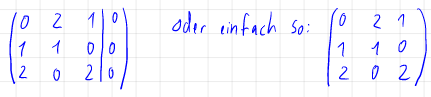
\includegraphics[width=.4\textwidth]{Dateien/00/11GaussC1.PNG}
\end{center}
Die zweite Schreibweise geht, da die rechte Seite der Gleichung (die Nullen) durch die Gauß-Operationen nicht geändert wird. Damit haben wir dann
\begin{center}
    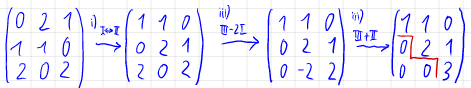
\includegraphics[width=.5\textwidth]{Dateien/00/11GaussC2.PNG}
\end{center}
Diese Gleichungen (also $3\lambda_3=0$, $2\lambda_2+\lambda_3=0$ und $\lambda_1+\lambda_2=0$) können tatsächlich nur durch $\lambda_1=\lambda_2=\lambda_3=0$ gelöst werden.\footnote{das kann man auch daran sehen, dass in der Zeilenstufenform keine Nullzeile mehr auftritt.}\\
Also ist die Familie $(v_i)_{i\in\{1,2,3\}}$ linear unabhängig.\\
Da die Anzahl der Elemente mit der Dimension 3 des $\mathbb{R}^3$ übereinstimmt, ist sie eine Basis des $\mathbb{R}^3$.
\end{Beispiel}
\begin{Beispiel}
{Lineare Unabhängigkeit und Basis prüfen (4/4)}
Bilden die folgenden Vektoren eine Basis des $\mathbb{R}^4$?
\begin{equation*}
    v_1=\Matrix{2\\-2\\6\\4},\quad v_2=\Matrix{1\\0\\2\\1},\quad v_3=\Matrix{2\\3\\0\\0},\quad v_4=\Matrix{1\\1\\1\\0}
\end{equation*}
Erneut: Gleichung für die lineare Abhängigkeit lösen:
\begin{equation*}
     \lambda_1v_1+\lambda_2v_2+\lambda_3v_3+\lambda_4v_4=\Vec{0}
\end{equation*}
\begin{center}
    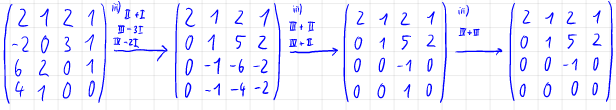
\includegraphics[width=.7\textwidth]{Dateien/00/11GaussD1.PNG}
\end{center}
Die letzte Gleichung lautet also $0\lambda_4=0$, d. h. wir können $\lambda_4$ beliebig wählen.\\
Wähle also $\lambda_4=:t\in\mathbb{R}\overset{(III)}{\Rightarrow}\boxed{\lambda_3=0}\overset{(II)}{\Rightarrow}\boxed{\lambda_2=-2t}\overset{(I)}{\Rightarrow}\boxed{\lambda_1=t/2}$.\\
Das Gleichungssystem wird also durch die Lösungsvektoren $L_t=t\Matrix{1/2\\-2\\0\\1}$ mit $t\in\mathbb{R}$ gelöst.\\
Betrachte als Beispiel $t=2:\quad v_1-4v_2+2v_4=\Vec{0}$ ist tatsächlich erfüllt.\\
Die Familie $(v_i)_{i\in\{1,2,3,4\}}$ ist also linear abhängig und kann daher kein Erzeugendensystem von $V$ sein.
\end{Beispiel}

\Tipps{1}{
\begin{enumerate}
    \item \begin{enumerate}
        \item Schaut euch die Definition der linearen Unabhängigkeit genau an - was folgt für die Koeffizienten von $\lambda_1v_1 +\lambda_2v_2=0$?
        \item Probiert verschiedene Beispiele aus, um ein Gefühl dafür zu bekommen.
    \end{enumerate}
    \item Denkt daran: Damit diese Funktionen linear unabhängig sind, müssen sie $\forall x\in \mathbb{R}$ linear unabhängig sein - vielleicht kann man daraus ja ein Gleichungssystem finden...\\
    Andererseits könnte es ja mit geschickten Koeffizienten ja auch klappen...
    \item Stumpfes Betrachten der Definition von linearen Abbildungen.
    \item
    \begin{enumerate}
        \item Hier müsst ihr einfach die Unterraumaxiome prüfen und schauen, was bei festem Grad schiefgehen könnte (etwa indem man durch Addition oder Multiplikation mit $\lambda\in\mathbb{R}$ außerhalb des Unterraums landet).
        \item Sollte schnell gemacht sein - evtl. hilft 3b).
        \item Hierfür einfach überlegen: Welche Polynome werden durch die zweite Ableitung auf den Nullvektor abgebildet? Diese bilden den Kern. Und: Auf welche Polynome wird ein Polynom von Grad $n$ durch die Abbildung abgebildet? Diese bilden das Bild. Gar nicht so schwierig, oder?
    \end{enumerate}
    \item \begin{enumerate}
        \item Schaut euch die Definition der inneren direkten Summe von Unterräumen an. Vielleicht ist der Durchschnitt ein guter Ansatz.
        \item Ein bisschen überlegen, wie nochmal die Dimension definiert war.
        \item Surjektivität bedeutet bei linearen Abbildungen $F:V\to W$, dass $\dim(\im(F))=\dim(W)$ ist.
        \item Injektivität bedeutet bei linearen Abbildungen, dass $\dim(\ker(F))=0$ ist, nur der Nullvektor aus $V$ wird also auf den Nullvektor aus $W$ abgebildet. Was ist hier aber der Nullvektor des Zielraumes?
    \end{enumerate}
\end{enumerate}} 
%%%%%%%%%%%%%%%%%%%%%%%%%%%%%%%%%%%%%%%%%%%%%%%%%%%%%%%%%%%%%%%%%
\newpage
\section[Lineare Abbildungen (Wdh. Mathe 1)]{Lineare Abbildungen, Dualraum, Matrizen}
\Einleitung{Abschließend schauen wir uns einen Spezialfall von Abbildungen zwischen Vektorräumen an: Die linearen Abbildungen.\\
Was macht diese so besonders?\\
Sie haben die schöne Eigenschaft, dass sie sich (bei endlichdimensionalen VR) stets als Matrizen darstellen lassen. Wie genau diese aussehen, hängt von den Basen der beteiligten Vektorräume ab!\\
Mit Matrizen kann man angenehm rechnen und viele Eigenschaften der Abbildung schnell überblicken.}\\
\red{Anmerkung: Diese Notizen sind anders als das Skript strukturiert, da wir das für sinnvoller hielten.}
\subsection{Lineare Abbildungen: Von Vektorraum zu Vektorraum mit Stil}\label{ssec:LineareAbbildungen}
\begin{Def}
{Lineare Abbildungen}
Wir nennen eine \red{Abbildung} $F$ zwischen zwei Vektorräumen\footnote{beide über dem gleichen Körper $\mathbb{K}$} $V$ und $W$, also $F:V\to W$ \red{$\mathbb{K}$-linear}, wenn sie die folgenden Eigenschaften für alle $v,w\in V$ und $\lambda\in\mathbb{K}$ erfüllt:
\begin{align*}
    F(v+w)&=F(v)+F(w)\\
    F(\lambda v)&=\lambda F(v).
\end{align*}
\end{Def}
\begin{Def}
{Wiederholung: Raum der Abbildungen}
Wie letzte Woche schon gesehen, können wir alle möglichen Abbildungen $A$ zwischen zwei Mengen $X$ und $Y$, d. h. $A:X\to Y$, als Vektorraum auffassen.\footnote{Das bedeutetet, dass Linearkombinationen dieser Abbildungen wieder solche Abbildungen sind.} Diesen hatten wir als $\Abb(X,Y)$ definiert.
\end{Def}
\blue{Dieses Konzept ist auf den ersten Blick sehr seltsam: Wir fassen Abbildungen als Vektoren auf und können somit auch Linearkombinationen (z. B. $5A-3B:X\to Y$ mit $A,B\in\Abb(X,Y)$) bilden.}
\begin{Def}
{Raum der $\mathbb{K}$-linearen Abbildungen}
Sind $V$ und $W$ wieder Vektorräume über $\mathbb{K}$, so stellen wir fest, dass alle linearen Abbildungen von $V\to W$ einen Unterraum von $\Abb(V,W)$ bilden.\\
Diesen bezeichnen wir als \red{$\boxed{L(V,W)}$}.
\end{Def}
Anstatt eine lineare Abbildung über '$F:V\to W$ linear' zu definieren, können wir einfach $F\in L(V,W)$ schreiben.
\begin{figure}[htbp]
\centering
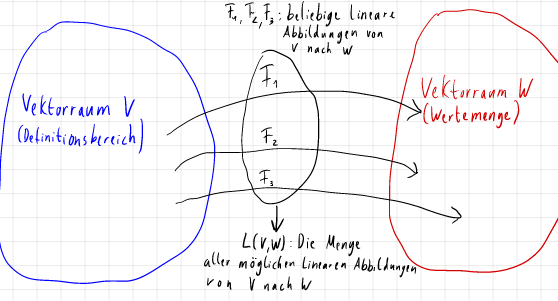
\includegraphics[width=.6\textwidth]{Dateien/00/12LinAbbSchaubild.PNG}
\caption*{Schaubild zu linearen Abbildungen. $\Abb(V,W)$ wäre hier noch eine größere Menge an Abbildungen als $L(V,W)$.}
\end{figure}
\begin{Beispiel}
{1D lineare Funktion (1/4)}
Für $V=\mathbb{R}$, $W=\mathbb{R}$ ist $F\in L(\mathbb{R},\mathbb{R}),\,F(x)=ax$ mit einer Konstante $a\in\mathbb{R}$ $\mathbb{R}$-linear, denn für alle $x,y\in V$, $\lambda\in\mathbb{R}$ gilt
\begin{align*}
    F(x+y)&=a(x+y)=ax+ay=F(x)+F(y)\\
    F(\lambda x)&=a\lambda x=\lambda ax=\lambda F(x).\, \checkmark
\end{align*}
\end{Beispiel}
\begin{Beispiel}
{Von 2D nach 1D (2/4)}
Für $V=\mathbb{R}^2$, $W=\mathbb{R}$ ist $F\in L(\mathbb{R}^2,\mathbb{R}),\,F\BracedIn{\Matrix{x\\y}}=F(x,y)=2x-7y$ $\mathbb{R}$-linear, denn für alle $v=\Matrix{x\\y},w=\Matrix{z\\a}\in \mathbb{R}^2$, $\lambda\in\mathbb{R}$ gilt
\begin{align*}
    F(v+w)&=F(x+z, y+a)=2(x+z)-7(y+a)=2x-7y+2z-7a=F(v)+F(w)\\
    F(\lambda v)&=F(\lambda x,\lambda y)=2\lambda x-7\lambda y y=\lambda(2x-7y)=\lambda F(v).\, \checkmark
\end{align*}
\end{Beispiel}
\begin{Beispiel}
{Quadratische Funktionen sind nicht linear (3/4)}
Die Abbildung $F\in\Abb(\mathbb{R},\mathbb{R}),\,F(x)=x^2$ ist nicht $\mathbb{R}$-linear, denn für $x=2\in\mathbb{R}$ gilt
\begin{align*}
    F(2+2)=4^2=16\neq 8=4+4=2^2+2^2=F(2)+F(2).\text{ \Lightning}
\end{align*}
\end{Beispiel}
\begin{Beispiel}
{Die Ableitung ist linear (4/4)}
Wie wir schon gesehen hatten, ist eine Eigenschaft der Ableitung\\
$A:C^1(\mathbb{R},\mathbb{R})\to C^0(\mathbb{R},\mathbb{R}),\, A(f)=f'$ die Linearität.\\
Da wir die stetig differenzierbaren Funktionen $C^1(\mathbb{R},\mathbb{R})$ und die stetigen Funktionen $C^0(\mathbb{R},\mathbb{R})$ als Vektorräume auffassen können, handelt es sich somit um eine lineare Abbildung.
\end{Beispiel}
Von nun an seien $U,V,W$ \underline{endlichdimensionale} Vektorräume über einem Körper $\mathbb{K}$. 
\begin{Satz}
{Satz}{Eindeutigkeit der Wirkung auf Basisvektoren}
Für $V,W$ mit $\dim V=n$ und mit einer festgelegten Basis $(b_1,b_2,...,b_n)$ von $V$ gibt es für jedes $n$-Tupel $(w_i)_{i=1,...,n}$ von Vektoren aus $W$ \underline{genau eine} lineare Abbildung mit $F(b_i)=w_i$.\\
Diese Abbildung ordnet also jedem Basisvektor aus $V$ einen der Vektoren aus dem Tupel zu und ist \underline{eindeutig}.
\end{Satz}
Dieser Satz ermöglicht später die Darstellung von $F$ über darstellende Matrizen bzgl. der Basen von $V$ und $W$ (siehe unten).
\begin{Satz}
{Satz}{Kompositionen linearer Abbildungen sind linear}
Seien $F\in L(U,V)$ und $G\in L(V,W)$.\\
Dann ist auch die Komposition $G\circ F:U\to W$ eine lineare Abbildung.
\end{Satz}
\begin{Satz}
{Satz}{Unterräume werden auf Unterräume abgebildet}
Sei $F\in L(V,W)$.\\
\begin{tabular}{c l}
\parbox[b]{8cm}{
Für jeden Unterraum $V'\subseteq V$ ist dessen Bild $F(V')\subseteq W$ ein Unterraum von $W$.\\
Zudem ist für jeden Unterraum $W'\subseteq W$ dessen Urbild $F^{-1}(W')\subseteq V$ ein Unterraum.\\
Im nebenstehenden Beispiel ist dies für eine Gerade, die ja ein Unterraum des $\mathbb{R}^2$ ist, veranschaulicht.
} & 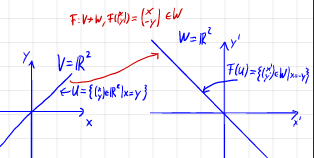
\includegraphics[width=.45\textwidth]{Dateien/00/12BeispielUnterraumUnterraum.PNG}
\end{tabular}
\end{Satz}
\subsubsection{Kern und Bild einer linearen Abbildung}\label{sssec:12KernBildDefinition}
Kennt ihr noch die grundlegenden Begriffe zu Abbildungen wie Injektivität und Surjektivität?\\
Diese werden nun wieder wichtig. Es stellt sich heraus, dass es aufgrund der Eigenschaften linearer Abbildungen ausreicht, zu schauen, ob nur der Nullvektor auf den Nullvektor abgebildet wird, um die Injektivität zu überprüfen.\\
So wie wir das Bild von allgemeinen Abbildungen kennengelernt hatten, interessiert uns nun das Bild von linearen Abbildungen. Stimmt die Dimension des Bildvektorraumes $F(V)$ mit der Dimension des Zielvektorraumes $W$ überein, so liegt Surjektivität vor. Diese Relationen greifen wir in Abschnitt \ref{ssec:Dimensionsformel} noch einmal auf, zunächst aber nur einige wichtige Definitionen:
\begin{Def}
{Kern von $F$}
Die Menge aller Vektoren aus $V$, die durch eine lineare Abbildung $F\in L(V,W)$ auf den \underline{Nullvektor} von $W$ abgebildet werden, nennen wir den \red{Kern von $F$}, geschrieben als\\
$\ker F= F^{-1}(\Vec{0})=\{v\in V\furdas F(v)=0\}\subseteq V$.
\end{Def}
\begin{Def}
{Bild von $F$}
Die Menge aller Vektoren aus $W$, die wir durch $F$ abbilden können, nennen wir das \red{Bild von F}, geschrieben als\\
$\im F=F(V)\subseteq W$.
\end{Def}
\blue{Aufgrund des vorhergehenden Satzes sind $\ker F\subseteq V$ und $\im F\subseteq W$ jeweils Unterräume von $V$ und $W$.}
\begin{figure}[htbp]
\centering
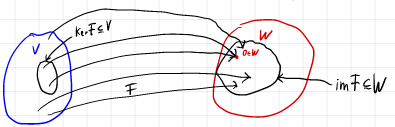
\includegraphics[width=.5\textwidth]{Dateien/00/12KernBild.PNG}
\caption*{Veranschaulichung von Kern und Bild}
\end{figure}
\subsection[Matrizen]{Matrizen\footnote{Laut \href{https://www.duden.de/rechtschreibung/Matrix}{Duden} ist die empfohlene Pluralschreibweise zwar Matrizes, aber irgendwie hört sich das komisch an - 'Matrizen' ist auch erlaubt.}}
Bevor wir tiefer in die linearen Abbildungen einsteigen, sollten wir uns mit ein paar zugrunde liegenden Definitionen vertraut machen.
\begin{Def}
{Matrix}
Wir definieren die Menge der \red{Matrizen} mit \red{$m$} Zeilen und \red{$n$} Spalten und Komponenten aus einem Körper $\mathbb{K}$ als
\begin{center}
    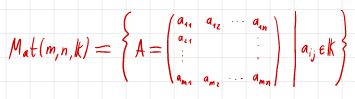
\includegraphics[width=.5\textwidth]{Dateien/00/12Matrixdefinition.PNG}
\end{center}
Mit der Notation $a_{ij}$ bezeichnen wir die insgesamt $m\cdot n$ Komponenten ($i=1,...,m$ und $j=1,...,n$).\\
Im Folgenden meint eine Einklammerung, dass alle Komponenten berücksichtigt werden, d. h. $(a_{ij}):=(a_{ij})_{i=1,...,m\, j=1,...,n}$.\\
Für $A=(a_{ij}), B=(b_{ij})\in\Met(m,n,\mathbb{K})$ und $\lambda\in\mathbb{K}$ bilden $(\Met(m,n,\mathbb{K}),+,\cdot, \mathbb{K})$ mit der Addition und der Multiplikation,
\begin{align*}
    +:&\quad(a_{ij})+(b_{ij})=(a_{ij}+b_{ij}),\\
    \cdot : & \quad\lambda (a_{ij})=(\lambda a_{ij})
\end{align*}
einen Vektorraum.
\end{Def}
\begin{Beispiel}
{Zeilenvektoren sind Matrizen (1/3)}
$A:=\Matrix{1 &2&3}\in\Met(1,3,\mathbb{R})$ ist eine $(1\times 3)$-Matrix.\\
Wir nennen $(1\times n)$-Matrizen auch \red{Zeilenvektoren}.
\end{Beispiel}
\begin{Beispiel}
{Spaltenvektoren sind Matrizen (2/3)}
$B:=\Matrix{-1\\0\\2}\in\Met(3,1,\mathbb{R})$ ist eine $(3\times 1)$-Matrix.\\
Wir nennen $(n\times 1)$-Matrizen auch \red{Spaltenvektoren}.
\end{Beispiel}
\begin{Beispiel}
{Linearkombination von Matrizen (3/3)}
$C:=\Matrix{1&3&4\\2&0&1}$ und $D:=\Matrix{-1&2&-2\\1.5&\pi &2}$ sind $(2\times 3)$-Matrizen. Es ist\\
\begin{equation*}
    -2C+D=\Matrix{-2&-6&-8\\-4&0&-2}+\Matrix{-1&2&-2\\1.5&\pi &2}=\Matrix{-3&-4&-10\\-2.5&\pi&0}.
\end{equation*}
\end{Beispiel}
\begin{Def}
{Matrixmultiplikation}
Seien $A=(a_{ij})\in\Met(m,n,\mathbb{K})$ und $B=(b_{ij})\in\Met(n,q,\mathbb{K})$.\\
Dann definieren wir als \red{Produkt} aus diesen Matrizen die Matrix
\begin{equation*}
    C=A\cdot B\in\Met(m,q,\mathbb{K}),\quad (c_{ik})=\sum_{j=1}^na_{ij}b_{jk}.
\end{equation*}
\end{Def}
\begin{Satz}
{Merksatz}{Mögliche Multiplikation}
Zum Testen, ob zwei Matrizen multiplizierbar sind, einfach die Dimensionen aufschreiben:
\begin{equation*}
    \boxed{m\times n\cdot p\times q}
\end{equation*}
ist nur möglich, wenn $n=p$.\\
Das Resultat ist eine $(m\times q)$-Matrix.
\end{Satz}
\begin{Beispiel}{Matrixmultiplikation}
Betrachte $C:=\Matrix{1&3&4\\2&0&1}$ und $D:=\Matrix{-1&2\\1&-1}.$\\
Welche Produkte sind möglich?
\begin{enumerate}
    \item $C\cdot D\rightarrow 2\times \overbrace{3\cdot 2}^{\neq} \times 2$. \Lightning
    \item $C^2\rightarrow 2\times \overbrace{3\cdot 2}^{\neq} \times 3$. \Lightning
    \item $D\cdot C\rightarrow 2\times \overbrace{2\cdot 2}^= \times 3\,\checkmark$ ($=2\times 3$). Hier ist
\begin{center}
    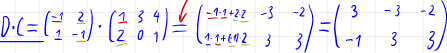
\includegraphics[width=.5\textwidth]{Dateien/00/12DMalC.PNG}
\end{center}
wobei ich (Fabian) mir den Schritt mit dem roten Pfeil immer so vorstelle, dass ich die einzelnen Spalten der hinteren Matrix auf die vordere draufklappe und damit die einzelnen Einträge bilde.
    \item $D^2\rightarrow 2\times \overbrace{2\cdot 2}^= \times 2\,\checkmark $ ($=2\times 2$). Hier haben wir
    \begin{equation*}
        D\cdot D=\Matrix{-1&2\\1&-1}\Matrix{-1&2\\1&-1}=\Matrix{1&-4\\-2&3}.
    \end{equation*}
\end{enumerate}
\end{Beispiel}
\begin{Def}
{Spur}
Für einige Anwendungen benötigt ihr später auch die \red{Spur}\footnote{engl. \textit{Trace}} von Matrizen.\\
Diese ist für quadratische Matrizen definiert und bezeichnet schlicht die Summe über alle Diagonalelemente:
\begin{equation*}
    \Tr:\Met(n,n,\mathbb{K})\to \mathbb{K},\quad A\mapsto \Tr(A)=\sum_{k=1}^na_{kk}.
\end{equation*}
\end{Def}
Die Spur findet vor allem in der Quantenmechanik Anwendung, wo mithilfe einer \textit{Dichtematrix} $\rho$ die Wahrscheinlichkeitsverteilung eines Systems widergespiegelt wird.\footnote{Siehe auch \href{https://de.wikipedia.org/wiki/Dichteoperator}{Wikipedia}.} Für die Normiertheit muss $\Tr(\rho)=1$ sein, die nicht-Diagonaleinträge symbolisieren die Übergangswahrscheinlichkeiten in andere Zustände.\\
Die Spur von $\rho^2$ gibt zudem Auskunft über die 'Reinheit' eines Systems.
\begin{Satz}
{Satz}{Vertauschbarkeit der Spur des Produktes}
Für $A\in\Met(m,n,\mathbb{K})$ und $B\in\Met(n,m,\mathbb{K})$ ist die Produktmatrix quadratisch.\\
Für deren Spur gilt
\begin{equation*}
    \Tr(\underbrace{A\cdot B}_{m\times m})=\Tr(\underbrace{B\cdot A}_{n\times n}).
\end{equation*}
Es lässt sich leicht zeigen, dass wir daher Matrizen innerhalb einer Spur zyklisch vertauschen können:\\
Für $A\in\Met(m,n,\mathbb{K})$, $B\in\Met(n,q,\mathbb{K})$ und $C\in\Met(q,m,\mathbb{K})$ gilt dann
\begin{equation*}
    \Tr(\underbrace{A\cdot B\cdot C}_{m\times m})=\Tr(\underbrace{C\cdot A\cdot B}_{q\times q})=\Tr(\underbrace{B\cdot C\cdot  A}_{n\times n}).
\end{equation*}
\end{Satz}


\subsubsection{Darstellende Matrizen: Lineare Abbildungen in Matrixdarstellung}
Nun erarbeiten wir uns die tolle Eigenschaft linearer Abbildungen, stets als Matrizen dargestellt werden zu können (zumindest, solange die beteiligten Vektorräume endlichdimensional sind).\\
Wie diese Matrizen aussehen, hängt aber von den Basen der Vektorräume ab! Daher wiederholen wir auch noch einmal den Basisbegriff.
\begin{Satz}
{Satz}{Kanonische Zuordnung}
Jeder linearen Abbildung $F\in L(\mathbb{K}^n,\mathbb{K}^m)$ können wir eine Matrix zuordnen, indem wir uns die \underline{Wirkung von $F$ auf die Basisvektoren} $(e_j)_{j=1,...,n}$ des $\mathbb{K}^n$ anschauen und diese als Matrix anordnen:
\begin{equation*}
    \varphi:L(\mathbb{K}^n,\mathbb{K}^m)\to \Met(m,n,\mathbb{K}),\, F\,\mapsto \varphi(F)=(F(e_1)\cdots F(e_n)).
\end{equation*}
\end{Satz}
\begin{Beispiel}{Kanonische Zuordnung}
Für $F:\mathbb{R}^2\to\mathbb{R}^3,\, F(x,y)=\Matrix{x+y\\2x-y\\5y}$ ist $F(e_1)=F(1,0)=\Matrix{1\\2\\0}$ und $F(e_2)=\Matrix{1\\-1\\5}$, wir haben also
\begin{equation*}
    \varphi(F)=\Matrix{1&1\\2&-1\\0&5}\in\Met(3,2,\mathbb{R}).
\end{equation*}
\end{Beispiel}
\begin{Def}
{Erinnerung: Basis}
Eine \red{Basis} eines Vektorraums $V$ der Dimension $\dim V= n$ ist eine linear unabhängige Familie von $n$ Vektoren, die den gesamten Vektorraum aufspannt,\footnote{alle Vektoren aus $V$ können also durch Linearkombination der Basisvektoren gebildet werden.} d. h. sie ist ein Erzeugendensystem von $V$.
\end{Def}
\begin{Beispiel}{Basen des $\mathbb{R}^3$}
Die Familien
\begin{align*}(e_1,e_2,e_3)&:=\BracedIn{\Matrix{1\\0\\0},\Matrix{0\\1\\0},\Matrix{0\\0\\1}},\\
(a_1,a_2,a_3)&:=\BracedIn{\Matrix{1\\1\\0},\Matrix{1\\0\\1},\Matrix{0\\-1\\-1}},\\
(b_1,b_2,b_3)&:=\BracedIn{\Matrix{1\\2\\3},\Matrix{4\\5\\6}\Matrix{7\\8\\-9}}
\end{align*}
sind jeweils Basen des $\mathbb{R}^3$.\\
Die Darstellung von Vektoren als Linearkombination hängt damit auch von der Basis ab:
\begin{equation*}
    v:=\Matrix{1\\1\\1}=e_1+e_2+e_3=\frac{1}{2}a_1+\frac{1}{2}a_2-\frac{1}{2}a_3=-\frac{1}{3}b_1+\frac{1}{3}b_2.
\end{equation*}
\end{Beispiel}
Wir haben gesehen, dass wir $F\in L(\mathbb{R}^n,\mathbb{R}^m)$ bzgl. der kanonischen Basis als Matrix darstellen können.\\
Dieses Konzept wollen wir nun auf lineare Abbildungen zwischen beliebigen (endlichdimensionalen) Vektorräumen $F\in L(V,W)$ mit beliebigen Basen von $V$ und $W$ erweitern.
\begin{Def}
{Darstellende Matrix}
Sei $B$ die Basis von $V$ (mit $\dim V=n$) und $B'$ die Basis von $W$ (mit $\dim W=m$).\\
Durch lineare Abbildungen $\phi_B:\mathbb{K}^n\to V,\,\phi_{B'}:\mathbb{K}^m\to W$, die so konstruiert sind, dass die kanonischen Einheitsvektoren des $\mathbb{K}^n$ bzw. $\mathbb{K}^m$ genau auf die Basen von $V$ und $W$ abgebildet werden, können wir $F$ durch den obigen Satz auf eine Matrix zurückführen:\\
Die \red{darstellende Matrix} $A\in\Met(m,n,\mathbb{K})$ bezüglich der Basen $B$ und $B'$ ist gegeben durch
\begin{equation*}
    Ae_j=(\phi^{-1}_{B'}\circ F\circ \phi_B)e_j
\end{equation*}
und wir schreiben $A=M_B^{B'}(F)$, um die verwendeten Basen zu verdeutlichen.\\
Für lineare Abbildungen $F\in L(\mathbb{K}^n,\mathbb{K}^m)$ nennen wir die darstellende Matrix bzgl. der Standardbasen die \red{kanonisch zugeordnete Matrix}.
\end{Def}
Das sieht auf den ersten Blick ziemlich kompliziert aus! Aber keine Angst, mit dem folgenden Satz kann man die darst. Matrix leicht finden, und es sollte auch noch klarer werden, wie man damit umgeht.
\begin{Satz}
{Satz}{Bestimmung der darstellenden Matrix}
Die darstellende Matrix $A=(a_{ij})=M_B^{B'}(F)$ einer linearen Abbildung $F\in L(V,W)$ ist durch folgende Gleichung bestimmt:
\begin{equation*}
    \boxed{F(b_{\red{k}})=\sum_{i=1}^ma_{i\red{k}}b'_i}.
\end{equation*}
Hierbei seien $b_k\in B$ Basisvektoren von $V$ und $b_i'\in B'$ die Basisvektoren von $W$.
\end{Satz}
\blue{Wir können also die darstellende Matrix einfach finden, indem wir uns die Wirkung von $F$ auf die Basisvektoren von $V$ anschauen und dann versuchen, die Matrixkomponenten als Koeffizienten der Linearkombinationen der Basisvektoren von $W$ zu finden.\footnote{Sorry für diesen Schachtelsatz, nach ein paar mal lesen oder vielleicht nach Betrachtung der Beispiele sollte er Sinn ergeben.}\\
\textbf{Anmerkung}: Für die Beispiele haben wir den eher anwendungsbezogenen zweiten Weg genommen. Falls euch interessiert, wie genau das mit den Abbildung $\phi_B$ und $\phi_{B'}$ aussehen würde, könnt ihr das in Abschnitt \ref{sssec:12DarstMatrixlang} nachlesen.}
\begin{Beispiel}
{Lineare Abbildung im $\mathbb{R}^2$ (1/2)}
\begin{tabular}{c l}
\parbox[b]{9cm}{
Wir betrachten $V=\mathbb{R}^2$, $W=\mathbb{R}^2$ und definieren die Basen
\begin{align*}
    B_V:&=(b_1,b_2)=\BracedIn{\Matrix{1\\1},\Matrix{-1\\1}},\\ B_W':&=(b_1',b_2')=\BracedIn{\Matrix{1\\3},\Matrix{2\\0}}.
\end{align*}
} & 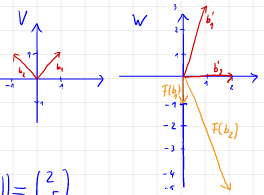
\includegraphics[width=.3\textwidth]{Dateien/00/12BeispielEbeneLinAbb.PNG}
\end{tabular}\\
Zudem sei unsere lineare Abbildung $F:V\to W$ durch
\begin{equation*}
    F(x,y)=\Matrix{y-x\\2x-3y}
\end{equation*}
definiert. 
\begin{itemize}
    \item Was macht $F$ mit den Basisvektoren von $V$?
    \begin{equation*}
        F(b_1)=F(1,1)=\Matrix{0\\-1},\quad F(b_2)=F(-1,1)=\Matrix{2\\-5}.
    \end{equation*}
    Um die darstellende Matrix bzgl. $B$ und $B'$ zu finden, müssen wir gucken, wie sich $F(b_1)$ und $F(b_2)$ durch $b_1'$ und $b_2'$ ausdrücken lassen.
    \item $F(b_1)$ und $F(b_2)$ als Linearkombination von $b_1'$ und $b_2'$:
    \begin{align*}
        \lambda_1b_1'+\lambda_2b_2'=F(b_1)&\Rightarrow \Matrix{1&2\\3&0}\Matrix{\lambda_1\\\lambda_2}=\Matrix{0\\-1}\rightarrow\lambda_1=-\frac{1}{3}\rightarrow\lambda_2=\frac{1}{6}\\
        \lambda_3b_1'+\lambda_4b_2'=F(b_1)&\Rightarrow \Matrix{1&2\\3&0}\Matrix{\lambda_3\\\lambda_4}=\Matrix{2\\-5}\rightarrow\lambda_3=-\frac{5}{3}\rightarrow\lambda_4=\frac{11}{6}
    \end{align*}
    Wir finden also:
    \begin{equation*}
        F(b_1)=-\frac{1}{3}b_1'+\frac{1}{6}b_2',\quad F(b_2)=-\frac{5}{3}b_1'+\frac{11}{6}b_2'.
    \end{equation*}
    \item Darstellende Matrix ablesen:\\
    Damit haben wir die Komponenten der darstellenden Matrix schon gefunden, denn es gilt ja 
\begin{equation*}
    \boxed{F(b_{\red{k}})=\sum_{i=1}^ma_{i\red{k}}b'_i}.
\end{equation*}
    Somit ist z. B. $F(b_1)=a_{11} b_1'+a_{21}b_2'$, also
    \begin{equation*}
        M_B^{B'}(F)=\Matrix{a_{11}&a_{12}\\a_{21}&a_{22}}=\Matrix{-1/3&-5/3\\1/6&11/6}=\frac{1}{6}\Matrix{-2&10\\1&11}.
    \end{equation*}
\end{itemize}
Und warum jetzt der ganze Aufwand?\\
Wir können jetzt beliebige Vektoren aus $V$, die wir bzgl. der Basis $B$ dargestellt haben, auf Vektoren bzgl. der Basis $B'$ aus $W$ abbilden!\\
Sei z. B. $v=\Matrix{3\\6}\in V$ bzgl. der Basis $B$,\footnote{Achtung, bzgl. der kanonischen Basis (wie ihr es vielleicht intuitiv kennt) sieht dieser Vektor anders aus!} d. h. $v=3b_1+6b_2$.\\
Dieser wird auf
\begin{equation*}
    w=M_B^{B'}(F)\cdot v=\frac{1}{6}\Matrix{-2&10\\1&11}\Matrix{3\\6}=\frac{1}{6}\Matrix{-6-60\\3+66}=\Matrix{-11\\23/2}
\end{equation*}
bzgl. der Basis $B'$, d. h. $w=-11b_1'+\frac{23}{2}b_2'$ abgebildet.
\begin{center}
    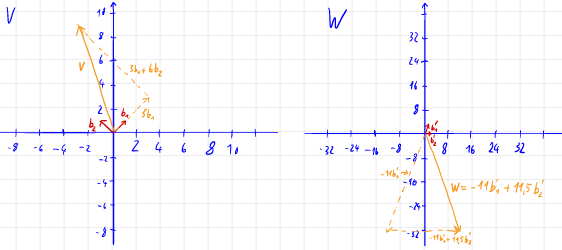
\includegraphics[width=.7\textwidth]{Dateien/00/12BeispielEbeneLinAbbB.PNG}
\end{center}
\textbf{Vergleich}:\\
Andererseits können wir $v$ und $w$ auch bzgl. der Standardbasen schreiben, denn dann sind
\begin{equation*}
    v=3b_1+6b_2=\Matrix{3-6\\3+6}=\Matrix{-3\\9},\quad w=-11b_1'+\frac{23}{2}b_2'=\Matrix{-11+23\\-33}=\Matrix{12\\-33}.
\end{equation*}
Wie sieht $F$ bzgl. der Standardbasen aus?\\ $F(e_1)=\Matrix{-1\\2}=-e_1'+2e_2'$ und $F(e_2)=\Matrix{1\\-3}=e_1'-3e_2'$.\\
Hier können wir die darstellende Matrix einfach ablesen, da die resultierenden Vektoren ja schon Linearkombinationen der kanonischen Einheitsvektoren von $W$ sind.
\begin{equation*}
    M_E^{E'}(F)=\Matrix{-1&1\\2 &-3}.
\end{equation*}
Und tatsächlich sehen wir:
\begin{equation*}
    F(v)=\Matrix{-1&1\\2 &-3}\Matrix{-3\\9}=\Matrix{12\\-33}=w.\,\checkmark
\end{equation*}
(Dafür bräuchten wir $M_E^{E'}$ eigentlich nicht, wir hätten auch $v$ einfach in $F$ einsetzen können.)
\end{Beispiel}
\begin{Beispiel}
{Der Link zum Vektorraum der Polynome (2/2)}\label{beisp:12DarstMatrix}
Sei $V=\mathbb{R}^2$ mit der Basis 
\begin{align*}
    B_V:&=(b_1,b_2)=\BracedIn{\Matrix{1\\1},\Matrix{-1\\1}}
\end{align*}
wie im vorherigen Beispiel.\\
Sei $W=\mathbb{R}[x]_{\leq 2}$ der 3-dimensionale Vektorraum der Polynome mit Grad $\leq2$ mit der Basis
\begin{equation*}
    B'=(b_1',b_2',b_3')=\BracedIn{(1+2x),(3x^2),(-x)}.
\end{equation*}
Sei unsere lineare Abbildung nun definiert als
\begin{equation*}
    F:\mathbb{R}^2\to \mathbb{R}[x]_{\leq 2},\,F(a,b)=a+(a-b)x+5bx^2\quad (\text{z. B. } F(1,2)=1-x+10x^2).
\end{equation*}
Wir notieren schonmal, dass diese Abbildung bzgl. der kanonischen Basen $E=(e_1,e_2)$ und $E'=(e_1',e_2',e_3')=((1),(x),(x^2))$ so aussieht:
\begin{equation*}
    M_E^{E'}(F)=\Matrix{1&0\\1&-1\\0&5}.
\end{equation*}
\begin{itemize}
    \item Was macht $F$ mit den Basisvektoren von $V$?
    \begin{eqnarray*}
        F(b_1)&=&F(1,1)\overset{\footnote{Einsetzungsweg}}{=}1+0x+5x^2=1+5x^2,\\
        F(b_2)&=&F(-1,1)\overset{\footnote{Bei gegebener darst. Matrix bzgl. der kanonischen Basen ist auch der Matrixmultiplikationsweg möglich.}}{=}\Matrix{1&0\\1&-1\\0&5}\Matrix{-1\\1}=\Matrix{-1\\-2\\5}=-1-2x+5x^2
    \end{eqnarray*}
    \item $F(b_1)$ und $F(b_2)$ als Linearkombination von $b_1'$, $b_2'$ und $b_3'$:\\
    Wir haben die Gleichungen
    \begin{equation*}
        \lambda_1b_1'+\lambda_2b_2'+\lambda_3b_3'=1+5x^2,\quad \lambda_4b_1'+\lambda_5b_2'+\lambda_6b_3'=-1-2x+5x^2,
    \end{equation*}
    die wir mit dem Gaußalgorithmus lösen können:
\begin{center}
    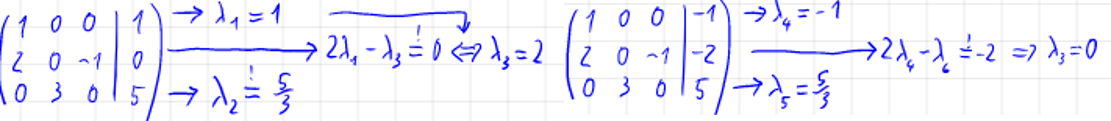
\includegraphics[width=.7\textwidth]{Dateien/00/12LsgGleichungssystem.png}
\end{center}
    \item Wir sehen also, dass
    \begin{equation*}
        1b_1'+\frac{5}{3}b_2'+2b_3'=1+5x^2,\quad -1b_1'+\frac{5}{3}b_2'+0b_3'=-1-2x+5x^2,
    \end{equation*}
    sodass wir die Koeffizienten für die darstellende Matrix nur noch ablesen brauchen:
    \begin{equation*}
        M_B^{B'}(F)=\Matrix{a_{11}&a_{12}\\a_{21}&a_{22}\\a_{31}&a_{32}}=\Matrix{1&-1\\5/3&5/3\\2&0}.
    \end{equation*}
    \item Anwendung:\\
    Wenn wir uns z. B. fragen, auf welchen Vektor $\in W$ der Vektor $v=2b_1-3b_2\in V$ abgebildet wird, reicht es, diesen mit $M_B^{B'}$ zu multiplizieren:
    \begin{align*}
        F(v)&=M_B^{B'}(F)\cdot v=\Matrix{1&-1\\5/3&5/3\\2&0}\Matrix{2\\-3}=\Matrix{5\\-5/3\\4}\\
        \Rightarrow w&=5b_1'-\frac{5}{3}b_2'+4b_3'=f(1+x)-\frac{5}{3}3x^2+4(-x)=5+6x-5x^2.
    \end{align*}
    Der Vergleich mit direktem Einsetzen liefert:
    \begin{equation*}
        F(v)=F\BracedIn{2\Matrix{1\\1}-3\Matrix{-1\\1}}=F(5,-1)=5+6x-5x^2.\,\checkmark
    \end{equation*}
\end{itemize}
\end{Beispiel}
\begin{Satz}
{Satz}{Verknüpfung linearer Abbildungen}
Seien $V,V',V''$ jeweils endlichdimensionale\footnote{da wir sonst ja keine darstellenden Matrizen definiert haben} Vektorräume mit den Basen $B,B',B''$. Seien $F\in L(V,V')$ und $G\in L(V',V'')$ lineare Abbildungen zwischen diesen Vektorräumen.\\
Dann ist $G\circ F\in L(V,V'')$ und für die darstellenden Matrizen gilt
\begin{equation*}
    M_B^{B''}(G\circ F)=M_{B'}^{B''}(G)M_B^{B'}(F).
\end{equation*}
\blue{Die darstellende Matrix einer verknüpften linearen Abbildung ist einfach das Produkt aus den darstellenden Matrizen der beteiligten Abbildungen.}
\end{Satz}
\begin{Beispiel}{Anwendung der Verknüpfung}\label{beisp:12VerknupfungLinAbb}
Seien $F:\mathbb{R}^3\to\mathbb{R},\,F(x,y,z)=3x+y-z$ und $G:\mathbb{R}\to \mathbb{R}^2,\,G(x)=\Matrix{2x\\-5x}$ lineare Abbildungen zwischen den Vektorräumen $\mathbb{R}^3,\mathbb{R},\mathbb{R}^2$ (mit den Basen $B,B',B''$).\\
Dann haben wir
\begin{equation*}
    (G\circ F):\mathbb{R}^3\to\mathbb{R}^2,\, (G\circ F)(x,y,z)=G(3x+y-z)=\Matrix{6x+2y-2z\\-15x-5y+5z}.
\end{equation*}
Seien $B,B',B''$ nun die Standardbasen von $\mathbb{R}^3,\mathbb{R},\mathbb{R}^2$. Dann ist
\begin{equation*}
    M_B^{B'}(F)=\Matrix{3 & 1 &-1},\quad M_{B'}^{B''}(G)=\Matrix{2\\-5}.
\end{equation*}
Deren Verknüpfung stimmt mit dem überein, was wir erwarten würden:
\begin{equation*}
    M_B^{B''}(G\circ F)=M_{B'}^{B''}(G)M_{B}^{B'}(F)=\Matrix{2\\-5}\cdot \Matrix{3&1&-1}=\Matrix{6&2&-2\\-15&-5&5}.\,\checkmark
\end{equation*}
\end{Beispiel}
\subsection{Zusammenhänge zwischen Rang, Dimension und Bijektivität}
Nun lernen wir eine wichtige Klassifikation von linearen Abbildungen kennen: Den sog. \textit{Rang}, der Auskunft über enorm viel gibt.\\
Wie sich herausstellen wird, können wir den bei Abbildungen zwischen endlichdimensionalen Vektorräumen einfach an der darstellenden Matrix ablesen, wenn wir diese auf Zeilenstufenform bringen. Auf geht's!\\
$V$ und $W$ seien im Folgenden weiterhin endlichdimensionale Vektorräume über $\mathbb{K}$.
\begin{Def}
{Rang einer Matrix}
Der \red{Rang} einer Matrix entspricht der \underline{Anzahl an linear unabhängigen Spalten} (bzw. Zeilen) der Matrix.\\
Also ist der Rang die Anzahl der Zeilen, die nach Anwendung des Gauß-Algorithmus nicht 0 werden.
\end{Def}
\begin{Def}
{Rang einer Abbildung}
Wir ordnen jeder linearen Abbildung $F:V\to W$ die \underline{positive}\footnote{inklusive 0} ganze Zahl
\begin{equation}
    \boxed{\rg F=\dim(\im F)}
\end{equation}
zu und nennen diese den \red{Rang von $F$}.\\
Der Rang entspricht also der Dimension des Bildes, und wir sehen schon, dass wir damit vielleicht einen Zusammenhang zur Surjektivität hergestellt haben.
\end{Def}
\begin{Satz}
{Satz}{Satz über den Rang}
Über die darstellende Matrix bzgl. beliebiger Basen $B,B'$ von $V$ und $W$ können wir diesen Rang bestimmen, denn es gilt
\begin{equation*}
    \rg F=\rg (M_B^{B'}(F)).
\end{equation*}
\blue{Interessanterweise hängt also das Aussehen der darst. Matrix von den Basen ab, der Rang ist aber invariant.}
\end{Satz}
\begin{Def}
{Transponieren einer Matrix}
Wir nennen eine an der Mitteldiagonalen gespiegelte Matrix $A^T$ die zu $A$ \red{transponierte} Matrix ($(a_{ij})^T=(a_{ji})$).\\
Das sieht dann z. B. so aus:
\begin{equation*}
    \Matrix{a&b\\c&d\\e&f}^T=\Matrix{a&c&e\\b&d&f}.
\end{equation*}
\end{Def}
\begin{Satz}
{Satz}{Zeilenrang {=} Spaltenrang}
Um den Rang einer Maxtrix zu bestimmen, ist es egal, ob wir diese \underline{transponieren}, bevor wir den Gauß-Algorithmus anwenden.
\end{Satz}
\begin{Beispiel}{Matrix mit vollem Rang (1/4)}
Die folgende Matrix hat $\rg A=3$:
\begin{equation*}
    A=\Matrix{1&0&0\\0&1&0\\0&0&1}.
\end{equation*}
\blue{Wenn keine Nullspalten/Zeilen auftreten, sagt man auch, die Matrix habe \red{vollen Rang}.}
\end{Beispiel}
\begin{Beispiel}{Matrix und Transponierte (2/4)}
Die folgende Matrix hat $\rg B= 2$, denn über den Gaußalgorithmus können wir sie umformen:
\begin{equation*}
    B=\Matrix{1&0&0\\0&1&1\\5&-5&-5}\overset{\text{Gauß}}{\rightarrow}\Matrix{1&0&0\\0&1&1\\0&0&0}.
\end{equation*}
Andererseits könnten wir auch
\begin{equation*}
    B^T=\Matrix{1&0&5\\0&1&-5\\0&1&-5}
\end{equation*}
betrachten, welche ebenfalls $\rg B^T=2$ hat.
\end{Beispiel}
\begin{Beispiel}
{Man sieht ihr den maximalen Rang an (3/4)}
Die folgende Matrix kann aufgrund des Satzes über das Transponieren maximal $\rg C\leq 2$ haben:
\begin{equation*}
    C=\Matrix{1&2\\3&4\\5&6}.
\end{equation*}
Betrachten wir $C^T$, so sehen wir:
\begin{equation*}
    C^T=\Matrix{1&3&5\\2&4&6}\overset{(II)-2(I)}{\to}\Matrix{1&3&5\\0&-2&-4}\Rightarrow\rg C^T=\rg C=2.
\end{equation*}
\end{Beispiel}
\begin{Beispiel}
{Rang einer verknüpften linearen Abbildung (4/4)}
Wir gucken uns wieder\\
$F:\mathbb{R}^3\to\mathbb{R},\,F(x,y,z)=3x+y-z$ und $G:\mathbb{R}\to \mathbb{R}^2,\,G(x)=\Matrix{2x\\-5x}$\\
(aus \hyperref[beisp:12VerknupfungLinAbb]{Bsp. 13.13}) an.\\
Da die Wahl der Basen für den Rang egal ist, wählen wir wieder die kanonischen Basen und haben
\begin{align*}
    \rg F&=\rg (M_B^{B'}(F))=\rg\Matrix{3&1&-1}=1\\
    \rg G &=\rg (M_{B'}^{B''}(G))=\rg \Matrix{2\\-5}=1\\
    \rg (G\circ F)&=\rg \Matrix{6&2&-2\\-15&-5 &5}\overset{(I)/2, (II)/5}{=}\rg \Matrix{3&1&-1\\-3&-1&1}\overset{(II)-(I)}{=}\rg\Matrix{3&1&-1\\0&0&0}=1.
\end{align*}
\end{Beispiel}
\subsubsection{Die Dimensionsformel und ihre Folgen}\label{ssec:Dimensionsformel}
\begin{Satz}
{Satz}{Dimensionsformel}
Für Vektorräume $V,W$ mit $\dim V=n\leq \infty$ und eine lineare Abbildung $F\in L(V,W)$ gilt:
\begin{equation*}
    \boxed{\rg F+\dim \ker F=\dim V}.
\end{equation*}
Die Dimension des Urbildraumes entspricht also der Summe aus der Dimension des Bildraumes und der Dimension des Raumes aller Vektoren aus $V$, die auf den Nullvektor abgebildet werden (vergl. Abschnitt \ref{sssec:12KernBildDefinition}).
\end{Satz}
\begin{Satz}
{Merksatz}{Surjektivität linearer Abbildungen}
Wie schon bei allgemeinen Abbildungen zwischen beliebigen Mengen nennen wir\\ $F\in L(V,W)$ \red{surjektiv}, wenn der gesamte Wertebereich getroffen wird, d. h. $F(V)=\im F\overset{!}{=}W$.\\
Aufgrund der Definition von $\rg F=\dim \im F$ gilt:
\begin{equation*}
    F\text{ surjektiv }\Leftrightarrow \rg F=\dim W.
\end{equation*}
\end{Satz}
\blue{Daraus folgen ein paar interessante Erkenntnisse:\\
$F$ kann nur surjektiv sein, wenn $\boxed{\dim V\geq \dim W}$.\\
Zudem ist das \underline{Bild der Basisvektoren} $(F(b_i))_i$ mit $(b_i)_i$ einer Basis von $V$ ein \underline{Erzeugendensystem} von $W$, wenn $F$ surjektiv ist.}
\begin{Satz}
{Merksatz}{Injektivität linearer Abbildungen}
Falls \underline{nur} der Nullvektor von $V$ durch $F\in L(V,W)$ auf den Nullvektor von $W$ abgebildet wird, d. h. $\ker F=\{\Vec{0}\}\subseteq V$, so ist $F$ \red{injektiv} (und umgekehrt).\\
Aufgrund der Dimensionsformel gilt dann (mit $\dim\ker F=0$)
\begin{equation*}
    F\text{ injektiv }\Leftrightarrow \rg F=\dim V.
\end{equation*}
\end{Satz}
\blue{Hier sehen wir nun:\\
$F$ kann nur injektiv sein, wenn $\boxed{\dim V\leq \dim W}$.\\
Zudem ist das \underline{Bild der Basisvektoren} $(F(b_i))_i$ \underline{linear unabhängig} in $W$, wenn $F$ injektiv ist.}
\subsubsection{Isomorphismen}\label{sssec:Isomorphismen}
Wir haben also nun schon einige Erkenntnisse zusammengetragen. Sicher könnt ihr nun 12 und 13 zusammenzählen und euch ausmalen, was besonderes passiert, wenn $\dim V=\dim W$ ist und sowohl Surjektivität als auch Injektivität von $F$ gegeben sind.
\begin{Def}
{Isomorphismus}
Wir nennen $F\in L(V,W)$ einen \red{Isomorphismus}, wenn $F$ \underline{injektiv und surjektiv} ist, d. h. $\ker F=\{0\}$ und $\im F=W$.\\
Für endlichdimensionale Vektorräume $V$ und $W$ gilt dann
\begin{equation*}
    F\text{ ist Isomorphismus }\Leftrightarrow \rg F\overset{\footnote{Dimensionsformel mit $\dim\ker F=0$}}{=}\dim V=\dim W.
\end{equation*}
\end{Def}
\blue{Zudem bildet das Bild der Basisvektoren $(F(b_i)_i)$ eine Basis\footnote{denn wie wir gesehen hatten sind diese Vektoren linear unabhängig aufgrund der Injektivität, und ein Erzeugendensystem aufgrund der Surjektivität.} von $W$, wenn $F$ bijektiv ist.}
\begin{Def}
{Isomorphie}
Wir nennen zwei Vektorräume $V$ und $W$ \red{isomorph}, wenn es einen Isomorphismmus von Vektorräumen gibt, d. h. wenn eine \underline{bijektive} lineare Abbildung $F:V\to W$ existiert.\\
\blue{Endlichdimensionale Vektorräume sind genau dann isomorph, wenn $\boxed{\dim V=\dim W}$.}
\end{Def}
\begin{Satz}
{Satz}{Linearität der Umkehrabbildung}
Ist $F:V\to W$ ein Isomorphismus, so ist die Umkehrabbildung $F^{-1}:W\to V$ ebenfalls linear.
\end{Satz}
\begin{Beispiel}
{Die Identitätsabbildung (1/4)}
Die (lineare) Identitätsabbildung $\Id: \mathbb{R}^n\to\mathbb{R}^n,\, \Id(x)=x$ ist ein Isomorphismus, denn die darstellende Matrix bzgl. der Standardbasen ist die $n\times n$-Einheitsmatrix
\begin{center}
    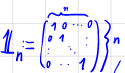
\includegraphics[width=.2\textwidth]{Dateien/00/12Einheitsmatrix.PNG}
\end{center}
weshalb $\rg F=\rg \mathds{1}_n=n=\dim\mathbb{R}^n=\dim\mathbb{R}^n$.
\end{Beispiel}
\begin{Beispiel}
{Verknüpfte Abbildung überprüfen (2/4)}
Wir gucken uns wieder\\
$F:\mathbb{R}^3\to\mathbb{R},\,F(x,y,z)=3x+y-z$ und $G:\mathbb{R}\to \mathbb{R}^2,\,G(x)=\Matrix{2x\\-5x}$\\
(aus \hyperref[beisp:12VerknupfungLinAbb]{Bsp. 13.13}) an.\\
Zunächst stellen wir fest, dass $F$ nicht injektiv sein kann, da $\dim \mathbb{R}^3>1=\dim \mathbb{R}$.\\
$G$ kann hingegen nicht surjektiv sein, da $\dim \mathbb{R}=1<2=\dim\mathbb{R}^2$.\\
Wir hatten gesehen, dass $\rg F=1$. Somit ist $F$ surjektiv.\\
Die Dimension des Kerns ist also nach der Dimensionsformel\\
$\dim\ker F=\dim \mathbb{R}^3-\rg F=2$.\\
\blue{Da der Kern ein Unterraum von $V$ ist, können wir dort auch eine Basis bestimmen. Dies schauen wir uns im nächsten Beispiel an.}\\
Es ist zudem $\rg G=1$. Somit ist $G$ injektiv (der Bildraum hat also ebenfalls eine Dimension von 1).\\
Die Verkettung $G\circ F:\mathbb{R}^3\to \mathbb{R}^2$ ist weder injektiv noch surjektiv, da\\
$\dim\mathbb{R}^3=3\neq1=\rg(G\circ F)$ (\Lightning Injektivität) und\\ $\dim \mathbb{R}^2=2\neq 1=\rg(G\circ F)$ (\Lightning Surjektivität).
\end{Beispiel}
\begin{Beispiel}
{Basis des Kerns bestimmen (3/4)}
Wir bestimmen jetzt eine Basis des Kerns von $F:\mathbb{R}^3\to\mathbb{R},\,F(x,y,z)=3x+y-z$, also dem Unterraum von $\mathbb{R}^3$, der von $F$ auf den Nullvektor abgebildet wird:
\begin{enumerate}
    \item \textbf{Gleichung aufstellen}:
    \begin{equation*}
        F(v)=\Vec{0}\overset{\footnote{Darst. Matrix bzgl. der Standardbasis}}{\to} \Matrix{3&1&-1}\Matrix{a\\b\\c}=0 \Leftrightarrow 3a+b-c=0.
    \end{equation*}
    \item \textbf{Koeffizienten bestimmen}:\\
    Dies ist \underline{eine} Gleichung mit \underline{drei} Unbekannten, d. h. wir dürfen \underline{zwei} Parameter frei wählen. Seien $a=:t\in\mathbb{R}$ und $b=:r\in\mathbb{R}$ diese Parameter.\\
    Dann ist $c=3t+r$.
    \item \textbf{Vektor aufschreiben}:\\
    Der Vektor $\Matrix{a\\b\\c}=\Matrix{t\\r\\3t+r}=t\Matrix{1\\0\\3}+r\Matrix{0\\1\\1}$ erfüllt die Gleichung, wird also von $F$ auf $0\in\mathbb{R}$ abgebildet.
    \item \textbf{Basis des Kerns ablesen}:\\
    Somit bilden die Vektoren $\Matrix{1\\0\\3}$ und $\Matrix{0\\1\\1}\in\mathbb{R}^3$ eine Basis des Kerns, wir haben also
    \begin{equation*}
        \ker F=\Spann{\Matrix{1\\0\\3},\Matrix{0\\1\\1}}.
    \end{equation*}
\end{enumerate}
Wie wir nach Betrachtung der Dimensionsformel gesehen hatten, ist also tatsächlich $\dim \ker F=2$.
\end{Beispiel}
\begin{Beispiel}[label=beisp:basisbildkern]
{Basis von Bild und Kern (4/4)}
Sei die lineare Abbildung $F:\mathbb{R}^4\to\mathbb{R}^3$ gegeben durch
\begin{equation*}
    \Matrix{a\\b\\c\\d}\mapsto\overbrace{\Matrix{1&-1&0&2\\4&-8&2&5\\-2&10&-4&2}}^{:=A}\overbrace{\Matrix{a\\b\\c\\d}}^{:=v}.
\end{equation*}
Wir wollen nun eine Basis des Kerns und eine Basis des Bildes bestimmen.\\
\textbf{Kern}:
\begin{enumerate}
    \item \textbf{Gleichungssystem aufstellen}:\\
    Wir wenden zunächst den Gaußalgorithmus an, um herauszufinden, welche Vektoren $\in\mathbb{R}^4$ auf $\Vec{0}\in\mathbb{R}^3$ abgebildet werden:
\begin{center}
    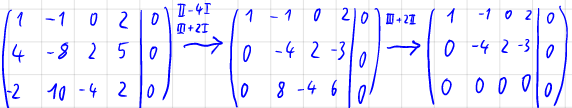
\includegraphics[width=.5\textwidth]{Dateien/00/12BasisKernGauss.PNG}
\end{center}
    \item \textbf{Koeffizienten bestimmen}:\\
    Wir können also $\dim \mathbb{R}^4-\rg A=4-2=2$ Variablen frei wählen.\\
    Seien $c=:r\in\mathbb{R}$ und $d=:t\in\mathbb{R}$. Es folgen die Gleichungen
    \begin{align*}
        -4b+2r-3t=0\Leftrightarrow b&=\frac{1}{2}r-\frac{3}{4}t\\
        a-\underbrace{\BracedIn{\frac{1}{2}r-\frac{3}{4}t}}_b+2t\Leftrightarrow a&=\frac{1}{2}r-\frac{11}{4}t.
    \end{align*}
    \item \textbf{Lösungsmenge aufschreiben}:\\
    Die Lösungsmenge des Gleichungssystems $F(v)=Av=0$ ist also
    \begin{equation*}
        L=\left\{r'\Matrix{1\\1\\2\\0}+t'\Matrix{-11\\-3\\0\\4}\furdas r',t'\in\mathbb{R}\right\},
    \end{equation*}
    wobei wir, da $r,t$ ja beliebig gewählt waren, diese noch skaliert haben.
    \item \textbf{Basis des Kerns ablesen}:\\
    Somit bilden die Vektoren $b_1=\Matrix{1\\1\\2\\0}$ und $b_2=\Matrix{-11\\-3\\0\\4}$ also eine Basis des Kerns von $F$. wir haben
    \begin{equation*}
        \ker F=\Spann{\Matrix{1\\1\\2\\0},\Matrix{-11\\-3\\0\\4}}.
    \end{equation*}
\end{enumerate}
\textbf{Bild}:\\
Das Bild muss aufgrund der Dimensionsformel\footnote{$\dim\im F=\rg F=\dim\mathbb{R}^4-\dim\ker F=4-2=2$} die Dimension 2 haben.\\
Alternativ können wir auch auf die darst. Matrix schauen und sehen, dass diese $\rg A=\rg F=2=\dim\im F$ hat.\\
Wenn wir uns nun also zwei linear unabhängige Spaltenvektoren aus $A$ schnappen, so bilden diese schon eine Basis von $\im F$, also z. B.
\begin{equation*}
    \im F=\Spann{\Matrix{1\\4\\-2},\Matrix{-1\\-8\\10}}.
\end{equation*}
Alternativ könnten wir die Spaltenvektoren als Zeilenvektoren aufschreiben und wieder Gauß anwenden:
\begin{center}
    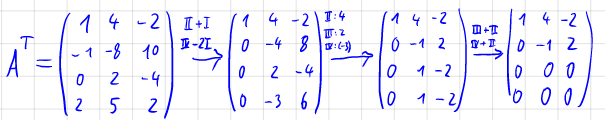
\includegraphics[width=.5\textwidth]{Dateien/00/12BildGauss.PNG}
\end{center}
Die alternative Basis des Bildes können wir nun einfach ablesen:
\begin{equation*}
    \im F=\Spann{\Matrix{1\\4\\-2},\Matrix{0\\-1\\2}}.
\end{equation*}
\end{Beispiel}
\subsubsection{Erneutes Vokabelgewitter}
Abschließend lernt ihr noch ein paar Begrifflichkeiten kennen, die spezielle lineare Abbildungen beschreiben. Diese werden vor allem nächstes Semester wichtig sein.
\begin{Def}
{Dualraum}
\begin{tabular}{c l}
\parbox[b]{10cm}{
Für jeden Vektorraum $V$ über einem Körper $\mathbb{K}$ bezeichnen wir die Menge aller linearen Abbildungen $V\to\mathbb{K}$ als \red{Dualraum $V^*:=L(V,\mathbb{K})$}.
} & 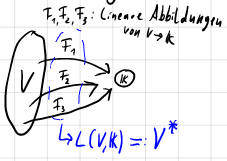
\includegraphics[width=.21\textwidth]{Dateien/00/12Dualraum.PNG}
\end{tabular}
\end{Def}
\begin{Def}
{Endomorphismus}
Lineare Abbildungen aus einem Vektorraum $V$ \underline{in sich selbst}, d. h. $F:V\to V$, nennen wir \red{Endomorphismen}.\\
Diese Menge\footnote{Die ja wieder ein Vektorraum ist, weil wir Linearkombinationen aus solchen Abbildungen bilden können, die wieder Vektoren sind} hat die Bezeichnung $\End(V):=L(V,V)$.\\
\blue{Auf endlichdimensionalen Vektorräumen mit $\dim V=n$ ist die darstellende Matrix dann eine $(n\times n)$-Matrix.}
\end{Def}
Die nächsten beiden Definitionen sind weitere Beispiele für Gruppen, welche wir im letzten Semester definiert hatten.
\begin{Def}{Automorphismus}
Ist ein Endomorphismus bijektiv (d. h. ein Isomorphismus), so nennen wir ihn \red{Automorphismus}.\\
Diese Menge hat die Bezeichnung $(\overbrace{\GL(V)}^{\footnote{Wenn $V$ endlichdimensional ist}}=)\Aut (V)\subseteq \End(V)$
Warum ist dies eine Gruppe?\\
Als Verknüpfung können wir die Komposition von Abbildungen verwenden, die aufgrund der Bijektivität alle erforderlichen Eigenschaften erfüllt. Automorphismen sind invertierbar. Die Identitätsabbildung ist das neutrale Element.\\
Diese Gruppe ist nicht kommutativ.
\end{Def}
\begin{Def}{Allgemeine lineare Gruppe (2/2)}
Ein Spezialfall tritt auf, wenn der Vektorraum $V$ \underline{endlichdimensional} ist.\\
Hier nennen wir Aut($V$) auch \red{GL($V$)}.\footnote{auch \textit{allgemeine lineare Gruppe} (\underline{G}eneral \underline{L}inear Group) genannt.}\\
Betrachte nun $V=\mathbb{K}^n$\footnote{Denn wie wir wissen, sind alle $n$-dimensionalen Vektorräume hierzu isomorph, d. h. es gibt eine bijektive lineare Abbildung zwischen $\mathbb{K}^n$ und diesen Räumen}.\\
In diesem Fall ist die darstellende Matrix der Automorphismen eine $n\times n$-Matrix.\\
Weil Automorphismen bijektiv sind, gilt\\ $\GL(V)=\{A\in\Met(n,\mathbb{K})\furdas \rg A=n\}=\{A\in\Met(n,\mathbb{K})\furdas \ker A=\{0\}\}=\{A\in\Met(n,\mathbb{K})\furdas \det A \neq 0\}$.\\
Es handelt sich also\footnote{bei endlichdimensionalen VR} genau dann um einen Automorphismus, wenn die darstellende Matrix invertierbar ist.
\end{Def}
\begin{Satz}
{Satz}{Vorgriff: Determinante und Isomorphie}
Für $(n\times n)$-Matrizen definieren wir bald die Determinante.\\
Diese gibt u.a. Auskunft darüber, ob der zugehörige Endomorphismus ein Automorphismus ist.\\
Ein Endomorphismus $F$ mit darst. Matrix $A$ ist genau dann auch ein Isomorphismus, wenn $\det(A)\neq 0$ ist.\\
Die Determinante ist eng mit dem Rang einer Matrix verknüpft.
\end{Satz}
\begin{figure}[htbp]
\centering
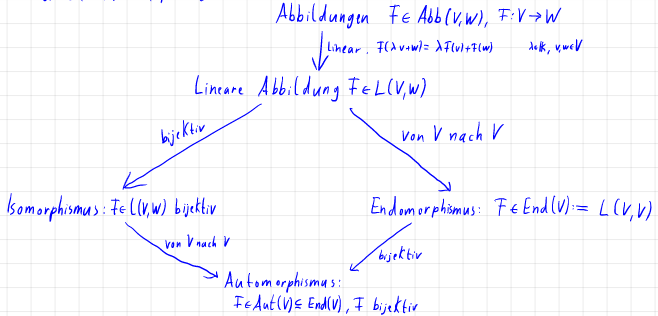
\includegraphics[width=.8\textwidth]{Dateien/00/12UbersichtBegriffe.PNG}
\caption*{Übersicht über die Zusammenhänge zwischen den Begriffen, die wir kennengelernt haben.}
\end{figure}

\subsection[Anhang]{Anhang: Betrachtung der $\phi_B$ und $\phi_{B'}$ aus Bsp. 12.11}\label{sssec:12DarstMatrixlang}
Dieser Anhang ist für alle von euch, die genauer interessiert, was eigentlich hinter den Kulissen abgeht. Meiner (Fabians) Meinung nach ist das nett zu wissen, aber keineswegs unentbehrlich.\\
Wir beziehen uns auf \hyperref[beisp:12DarstMatrix]{Bsp. 12.11}, wo wir ja die darstellende Matrix von $F:\mathbb{R}^2\to\mathbb{R}[x]_{\leq2}=:F:V\to W$ finden wollten.\\
Dort hatten wir 
\begin{equation*}
    F:\mathbb{R}^2\to \mathbb{R}[x]_{\leq 2},\,F(a,b)=a+(a-b)x+5bx^2\quad (\text{z. B. } F(1,2)=1-x+10x^2).
\end{equation*}
Wie sehen nun die Abbildungen $\phi_B$ und $\phi_{B'}$ aus der Definition der darst. Matrix aus?\\
Diese sollen nun Abbildungen aus $\mathbb{R}^2\to V$ bzw. $\mathbb{R}^3\to W$ sein, sodass die kanonischen Einheitsvektoren von $\mathbb{R}^2$ bzw. $\mathbb{R}^3$ auf $B$ bzw. $B'$ abgebildet werden.
\begin{itemize}
    \item Für $\phi_B:\mathbb{R}^2\to V$ haben wir:\\
    $\phi_B(e_j)\overset{!}{=}b_j$. Die kanonische Matrix dieser Abbildung ist:
    \begin{equation*}
        A_{\phi_B}=\Matrix{1&-1\\1&1},\text{ denn } A_{\phi_B}e_1=\Matrix{1\\1}=b_1\text{ und } A_{\phi_B}e_2=\Matrix{-1\\1}=b_2.\,\checkmark
    \end{equation*}
    \item Analog haben wir für $\phi_{B'}:\mathbb{R}^3\to W$
    \begin{equation*}
        A_{\phi_{B'}}=\Matrix{1&0&0\\2&0&-1\\0&3&0}, \text{ denn } A_{\phi_{B'}}e_1=\Matrix{1\\2\\0}\overset{\wedge}{=}1+2x=b_1,\text{ Rest analog}.\,\checkmark
    \end{equation*}
    \item Für die Anwendung benötigen wir nun die Umkehrabbildung $\phi_{B'}^{-1}:W\to\mathbb{R}^3$:
    \begin{equation*}
        A_{\phi_{B'}}^{-1}=\Matrix{1&0&0\\0&0&1/3\\2&-1&0}.
    \end{equation*}
    \blue{\textbf{Anmerkung}: Das Werkzeug zum Invertieren von Matrizen erhaltet ihr im zweiten Semester. Keine Angst, das müsst ihr aktuell nicht können.}
    \item Damit ist die darstellende Matrix in ihren einzelnen Komponenten also
    \begin{align*}
        j=1:&\quad A e_1=\phi_{B'}^{-1}(F(\phi_B(e_1)))=\phi_{B'}^{-1}(F(1,1))=\Matrix{1&0&0\\0&0&1/3\\2&-1&0}\Matrix{1\\0\\5}=\Matrix{1\\5/3\\2}\\
        j=2:&\quad A e_2=\phi_{B'}^{-1}(F(\phi_B(e_2)))=\phi_{B'}^{-1}(F(-1,1))=\Matrix{1&0&0\\0&0&1/3\\2&-1&0}\Matrix{-1\\-2\\5}=\Matrix{-1\\5/3\\0}.
    \end{align*}
    \item Also ist $M_B^{B'}(F)$ (wie schon oben herausgefunden) einfach
    \begin{equation*}
        M_B^{B'}(F)=\Matrix{1&-1\\5/3&5/3\\2&0}.
    \end{equation*}
\end{itemize}


\subsection{Äquivalenzrelationen und Orientierung}
\blue{Bevor wir uns dem nächsten großen Thema, den \red{Eigenvektoren}, widmen, folgt nun ein kurzer Überblick über das Konzept der Äquivalenzrelationen, den Quotientenraum und die Orientierung von Basen.}
\begin{Wiederholung}
{Relation}
Eine \red{Relation} $R$ auf einer Menge $X$ kann als Teilmenge von $X\times X$ aufgefasst werden.\\
Diese Teilmenge umfasst dann alle Paare $(x,y)\in X\times X$, für die die Relation erfüllt ist.
\end{Wiederholung}
Bereits bekannte Relationen sind die \red{Ordnungsrelationen} ($>,<,\leq,\geq,=$), aber wir können natürlich auch jegliche andere Paare definieren, z.B. die Relation $\hat{R}_2$ auf $\mathbb{N}$, die alle natürlichen Zahlen verknüpft, die das durch den Faktor 2 verbunden werden, d.h.\\
$\hat{R}_2:=\Menge{(x,y)\in\mathbb{N}^2}{x=2y\lor y=2x}$.\\
Von diesen allgemeinen Relationen betrachten wir nun einen Spezialfall:
\begin{Def}
{Äquivalenzrelation}
Wir nennen eine Relation $\sim$ auf einer Menge $X$ eine \red{Äquivalenzrelation}, wenn sie folgende drei Eigenschaften erfüllt:\\
\begin{tabularx}{\linewidth}{p{2.2cm}|X|X}
    \textbf{Name} &\textbf{Forderung}&\textbf{Erklärung} \\
    \hline
    \blue{Reflexivität:} & $x\sim x\,\forall x\in X$ & $x$ ist zu sich selbst äquivalent.\\
    \hline
    \blue{Symmetrie:} & $x\sim y\implies y\sim x\,\forall x,y\in X$ & Ist $y$ zu $x$ äquivalent, so ist auch $x$ zu $y$ äquivalent.\\
    \hline
    \blue{Transitivität:}  & $x\sim y\land y\sim z\implies x\sim z\,\forall x,y,z\in X$ & Sind $x$ und $y$ und zudem $y$ und $z$ äquivalent, so sind auch $x$ und $z$ äquivalent.
\end{tabularx}
\end{Def}
\begin{Def}
{Äquivalenzklasse}
Gemeinsam mit der Äquivalenzrelation $\sim$ definiert jedes Element aus $X$ dann eine \red{Äquivalenzklasse $[x]$}:
\begin{equation}
    [x]:=\Menge{y\in X}{y\sim x},
\end{equation}
diese beinhaltet also alle Elemente aus $X$, die zu $x$ äquivalent sind.\\
Als $X/\sim$ bezeichnen wir die Menge aller möglichen Äquivalenzklassen.
\end{Def}
\begin{Beispiel}
{Geburtsjahräquivalenz (1/3)}
Für die Menge aller Studierenden an der Physikfakultät ist \textit{das gleiche Geburtsjahr haben} eine Äquivalenzrelation. Die Menge aller möglichen Äquivalenzklassen würde in diesem Fall alle vertretenen Geburtsjahre beinhalten.\\
Andere Äquivalenzrelationen wären der Geburtsort oder andere eindeutige Eigenschaften der Studierenden.
\end{Beispiel}
\begin{Beispiel}
{Restklassen (2/3)}
Wir betrachten die Menge $X=\mathbb{Z}$ der ganzen Zahlen und eine natürliche Zahl $n>1$.\\
Durch 
\begin{equation*}
    x\sim y\iff n\tx{ teilt }(x-y)
\end{equation*}
wird dann eine Äquivalenzrelation auf $\mathbb{Z}$ definiert.\footnote{Als Beispiel sei $n=3$ genannt. In diesem Fall sind 5 und 8 äquivalent, 5 und 9 aber nicht.} Zwei ganze Zahlen sind hier also genau dann äquivalent, wenn sie bei Division durch $n$ den selben Rest lassen.\\
Mit $\mathbb{Z}/n\mathbb{Z}$ oder einfach $\mathbb{Z}_n$ bezeichnet man die Menge der \red{Restklassen}, also die Klassen, die durch den Rest bei Division durch $n$ definiert sind.\\
Diese Klassen kann man durch
\begin{equation*}
    [x]+[y]:=[x+y]\quad \tx{und}\quad [x]\cdot [y]:=[x\cdot y]
\end{equation*}
mit einer Addition und Multiplikation versehen, sodass $(\mathbb{Z}_n,+)$ eine kommutative Gruppe mit neutralem Element $[0]$\footnote{also die Äquivalenzklasse, die alle Zahlen enthält, die durch $n$ ohne Rest teilbar sind} ist.\\
Falls $p$ eine Primzahl ist, ist $(\mathbb{Z}_p,+,\cdot)$ sogar ein Körper (mit dem neutralen Element der Multiplikation $[1]$).
\end{Beispiel}
\begin{Beispiel}
{Die Betragsäquivalenz}
\begin{wrapfigure}{r}[0pt]{.25\textwidth}
 \vspace{-15pt}
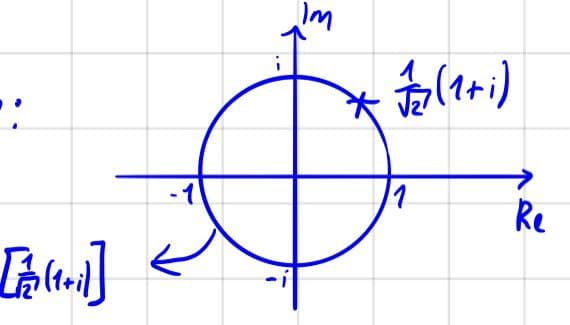
\includegraphics[width=.25\textwidth]{Dateien/01/01Betragsklassen.jpg}
 \vspace{-15pt}
\end{wrapfigure}
Auf den komplexen Zahlen sei $x\sim y\iff \Abs{x}=\Abs{y}$ mit $x,y\in\mathbb{C}$.\\
Dies ist eine Äquivalenzrelation, denn die Reflexivität ist klar, die Symmetrie folgt aus der Symmetrie des Betrages und die Transitivität folgt aus der Transitivität der Gleichheit.\\
Äquivalenzklassen sind dann Kreise in der komplexen Ebene, im Bild seht ihr die Äquivalenzklasse $[\frac{1}{\sqrt{2}}(1+i)]$.\\
Die Menge aller Äquivalenzklassen $\mathbb{C}\,\setminus\sim$ entspricht dann z.B. allen positiven reellen Zahlen, da diese jeweils einzigartige Äquivalenzklassen definieren.
\end{Beispiel}
Das Konzept der Äquivalenzklassen nutzen wir nun, um Äquivalenz zwischen Vektoren in Bezug auf einen Untervektorraum herzustellen:
\begin{Def}
{Quotientenraum}
Für Unterräume $U\subseteq V$ eines Vektorraums $V$ über einem Körper $\mathbb{K}$ können wir (auf $V$!) eine Äquivalenzrelation für Vektoren $v,w\in V$ definieren:
\begin{equation}
    v\sim w\iff v-w=u\in U.
\end{equation}
Die Menge $V/U=\Menge{[v]}{v\in V}$ aller Äquivalenzklassen\footnote{z.B. die zu $U$ parallelen Geraden, siehe im folgenden Beispiel} nennen wir auch \red{Quotientenraum} oder \red{Quotientenvektorraum}\footnote{Siehe auch unter \href{https://de.wikipedia.org/wiki/Faktorraum}{Wikipedia}.} von $U$.
\end{Def}
Was bedeutet diese Relation anschaulich?\\
Wir klassifizieren Vektoren $v,w\in V$ als gleich, sobald ihre Differenz im Unterraum $U$ liegt. Umgeschrieben können wir $w=u+v$ schreiben, $v$ und $w$ sind also äquivalent, wenn man durch Verschiebung von $v$ um einen Vektor aus $U$ den Vektor $w$ erzeugen kann. Dies wird vielleicht mit einem Beispiel verständlicher:
\begin{Beispiel}
{Quotientenraum im $\mathbb{R}^2$}
\begin{wrapfigure}{r}[0pt]{.35\textwidth}
 \vspace{-15pt}
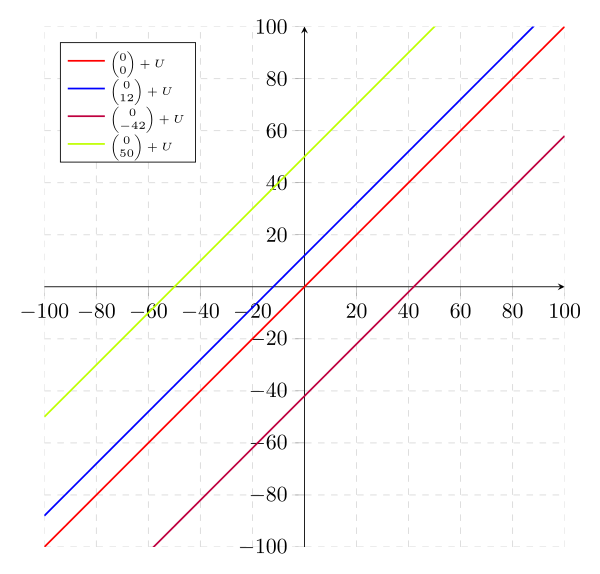
\includegraphics[width=.35\textwidth]{Dateien/01/01Quotientenraum.png}
\end{wrapfigure}
Sei $V=\mathbb{R}^2$ und $U$ eine Gerade mit\\
$U=\Menge{v\in V}{v=\MatrixInline{1\\1}x,\, x\in \mathbb{R}}$.\\
Dann sind mit $\sim$ alle Punkte, die jeweils auf einer Geraden parallel zu $U$ liegen zueinander äquivalent und wir können für die Äquivalenzklassen eines Vektors $v$ auch schreiben
\begin{equation*}
    [v]=\Menge{w\in V}{w=v+u,\,u\in U}.
\end{equation*}
Dies ist im nebenstehenden Bild (von Wikipedia) illustriert.
\end{Beispiel}



\Tipps{2}{
\begin{enumerate}
\item Orientiert euch an unseren Beispielen zur Basisfindung im Kapitel zu Vektorräumen.
\item Hierzu haben wir z. B. Beispiel \ref{beisp:basisbildkern} angesehen.
\item Schlagt hier die genauen Definitionen der Linearität und der Matrixmultiplikation nach, dann dürfte das nicht sonderlich umfangreich sein. Für c) könnte b) vielleicht nützlich sein.
\item Schaut bei Problemen gern die Hilfestellungen und Beispiele zu Äquivalenzrelationen an. Hier müsst ihr einfach stumpf die Eigenschaften überprüfen oder euch überlegen, weshalb eine davon nicht klappt.
\end{enumerate}
}
%%%%%%%%%%%%%%%%%%%%%%%%%%%%%%%%%%%%%%%%%%%%%%%%%%%%%%%%%%%%%%%%%
\newpage
\section[Determinanten]{Determinanten}
\Einleitung{Ein zentrales Thema in diesem Semester sind Determinanten, für die wir mit der Betrachtung von Gruppen ja schon die Vorarbeit geleistet hatten.\\ Letzte Woche hatten wir Endomorphismen als einen Spezialfall der linearen Abbildungen kennengelernt - diese bilden aus einem Vektorraum $V$ wieder nach $V$ ab!\\
Bei Anwendung des gaußschen Algorithmus auf die darstellende Matrix von Endomorphismen (diese ist quadratisch!) ergibt sich auf natürliche Weise ein Objekt, mit dem wir die Endomorphismen charakterisieren können: Die Determinante.\\
Bereits nächste Woche werden wir sehen, dass die Determinante bei der Bestimmung spezieller mit linearen Abbildungen verknüpfter Werte nützlich ist.\\
Zudem schauen wir uns an, wie man Matrizen invertieren kann und welche Feinheiten man dabei beachten muss.}
\subsection{Hinführung}
Wir versuchen, uns dem am Anfang sehr abstrakten Konzept der Determinante anhand von zwei Problemen zu nähern, sodass die Definition sinnvoll erscheint:\\
Betrachtet man Endomorphismen,\footnote{zunächst einmal auf einem endlichdimensionalen Vektorraum $V$, da wir sonst keine darstellenden Matrizen mehr finden können} so stellt sich schnell die Frage, wie man (wenn überhaupt) eine Umkehrabbildung finden kann. Diese Fragestellung können wir auf die Inversion der darstellenden Matrix zurückführen. Lasst uns dazu ein Beispiel betrachten:
\begin{Beispiel}
{Invertieren einer Matrix}
Wir betrachten eine lineare Abbildung $F:\mathbb{R}^2\to\mathbb{R}^2$, die durch
\begin{equation*}
    F\Matrix{x\\y}=A\Matrix{x\\y}=\Matrix{a&b\\c&d}\Matrix{x\\y}=\Matrix{x'\\y'}
\end{equation*}
definiert sei. Hierbei sei $A$ die darstellende ($2\times 2$)-Matrix bezüglich der kanonischen Basis.\\
Wir können uns stattdessen auch das folgende lineare Gleichungssystem angucken:
\begin{eqnarray*}
    I:&\quad&ax+by=x'\\
    II:&\quad&cx+dy=y'
\end{eqnarray*}
anschauen. Eine Inversion der Matrix entspricht dem Umstellen dieses Systems nach $x$ und $y$. Probiert euch selbst gern daran, ihr solltet schließlich bei
\begin{eqnarray*}
I:&\quad& x=\frac{1}{ad-bc}(dx'-by')\\
II:&\quad &y=\frac{1}{ad-bc}(-cx'+ay')
\end{eqnarray*}
herauskommen,\footnote{Unten haben wir dieses Ergebnis noch einmal als \textit{Cramersche Regel} festgehalten.} sodass wir in Matrixdarstellung die Form
\begin{equation*}
    \Matrix{x\\y}=\frac{1}{ad-bc}\Matrix{d&-b\\-c&a}\Matrix{x'\\y'}=:\frac{1}{\det A}\Matrix{d&-b\\-c&a}\Matrix{x'\\y'}
\end{equation*}
Diesen Vorfaktor identifizieren wir mit der Determinante, wir haben also
\begin{equation}
    \det A=\det\Matrix{a&b\\c&d}=ad-bc.
\end{equation}
Für diese $2\times2$-Matrix war das ja noch entspannt, aber auch beim Invertieren von anderen $n\times n$-Matrizen taucht sie auf.
\end{Beispiel}
\blue{Hier taucht die Determinante im Nenner auf. Dies ist ein erstes Zeichen, dass wir aufpassen müssen, wenn $\det A=0$ ist. In diesem Fall sind Matrizen nicht invertierbar und lineare Gleichungssysteme nicht mehr garantiert lösbar.}
\begin{Beispiel}{Anwendung des Gauß-Algorithmus}
Genauso taucht die Determinante auf, wenn wir den Gauß-Algorithmus auf die Matrix anwenden:
\begin{equation}
    \Matrix{a&b\\c&d}\overset{(II)\cdot a-c\cdot(I)}{\longrightarrow}\Matrix{a&b\\0&ad-bc}=\Matrix{a&b\\0&\det A}
\end{equation}
Diese Umformungen verwenden wir auch, wenn wir ein Gleichungssystem der Form $Ax=b$ lösen.\\
Dieses Prinzip können wir auf eine $n\times n$-Matrix erweitern und erhalten ganz analog als letzten Eintrag die Determinante:
\begin{center}
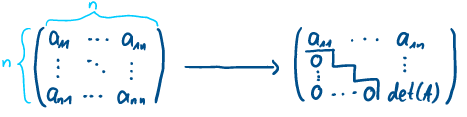
\includegraphics[width=.5\textwidth]{Dateien/00/14DeterminanteNKreuzN.PNG}
\end{center}
Leider wird es hierbei aber schnell sehr kompliziert, die Determinante zu berechnen.
\end{Beispiel}
\begin{Satz}{Rechenregel}{Cramersche Regel}
Wir halten fest:\\
Ein Gleichungssystem der Form $A\xvec=\bvec$, wobei\\ $A=\Matrix{a&b\\c&d}\in\Met(2,\mathbb{K})$ und $\bvec=\Matrix{e\\f}\in\mathbb{K}^2$, bzw.
\begin{equation*}
    ax+by=e,\quad cx+dy=f,
\end{equation*}
wird (falls $\det A=ad-bc\neq0$) gelöst durch
\begin{align*}
    x=\frac{1}{\det A}(ed-bf)\\
    y=\frac{1}{\det A}(af-ce).
\end{align*}
\end{Satz}
Ein weiteres Beispiel (das Volumen eines Parallelotops) findet ihr im Anhang dieses Kapitels, Abschnitt \ref{ssec:14AnhangParallelotop}.



\subsection{Kurze Wiederholung zu Gruppen und deren Anwendung}
Auch wenn ihr letztes Semester bereits die wichtigsten Begriffe für Gruppen kennengelernt habt, wollen wir, bevor es richtig losgeht, hier nochmal daran erinnern. Diese neue algebraische Struktur (neben Körpern und Vektorräumen) braucht ihr im Rahmen der Mathevorlesungen vor allem zur präzisen Formulierung der Determinanten. Aber auch in der Physik spielen sie eine tragende Rolle, zum Beispiel wenn es um die Beschreibung von Symmetrien (Drehung, Verschiebung, Spiegelung etc.) geht. Daher handelt es sich hier keineswegs um ein Nischenthema sondern um ein mathematisches Werkzeug, dass zu immensen Fortschritten im Verständnis der Natur geführt hat. \\

Also dann legen wir mal los: was war denn noch gleich eine Gruppe? Dazu schauen wir uns erstmal die trockene Definition an:
\begin{Wiederholung}
{Gruppen}
Eine Gruppe besteht aus einer Menge $G$ und einer Verknüpfung $\cdot:G\times G \mapsto G$, die folgende Eigenschaften erfüllen: \\

\begin{itemize}
    \item $(u\cdot v)\cdot w = u\cdot (v\cdot w) \qquad \forall u,v,w \in G$ \qquad (Assoziativität)
    \item $\exists e\in G: u\cdot e = e\cdot u = u \qquad \forall u\in G$ \qquad (Existenz des neutralen Elements)
    \item $\forall u\in G \, \exists u^{-1} \in G\,: u\cdot u^{-1} = u^{-1} \cdot u = e$ \qquad (Existenz des inversen Elements) \\
\end{itemize} 

Ist die Verknüpfung zusätzlich noch kommutativ, spricht man von einer \red{abelschen Gruppe}.
\end{Wiederholung}
Wie sehen jetzt aber Mengen aus, die diese Voraussetzungen erfüllen und was macht sie so besonders? Dazu schauen wir und mal ein paar Beispiele an, die ihr auch schon aus dem letzten Semester kennen solltet:
\begin{Beispiel}
{Besondere Gruppen}
\begin{enumerate}
    \item Bijektive Abbildungen bilden zusammen mit der Komposition \glqq $\circ$ \grqq eine Gruppe. Dass die Komposition Assoziativität erfüllt, haben wir in Mathe 1 gesehen. Mit der Identität $\Id$ und der Umkehrabbildung sind auch neutrales und inverses Element gegeben. Wir schreiben die Gruppe als:
    \begin{equation*}
        \Bij(X)=\Menge{\varphi : X \rightarrow X}{\varphi \text{ bijektiv}}.
    \end{equation*}
    Ist $X$ eine endliche Menge, nennt man $\sigma \in \Bij(X)$ eine \red{Permutation}.
    \item Die symmetrische Gruppe \red{(wichtig!)} ist definiert als
    \begin{equation*}
        S_{n} = \Bij(\{1,...,n\}).
    \end{equation*}
    Sie enthält Abbildungen, die alle n Elemente einer Gruppe nehmen und umordnen (permutieren).
    \item Ist $X=V$ ein Vektorraum, nennt man 
    \begin{equation*}
        \Aut(V) = \Bij(V)
    \end{equation*}
    die Automorphismengruppe.
    \item Ist $V$ endlichdimensional, dann ist 
    \begin{equation*}
        \GL(V) = \Aut (V)
    \end{equation*}
    die allgemeine lineare Gruppe (\underline{G}eneral \underline{L}inear Group).
    Ist $V=\mathbb{K}^{n}$, dann gilt:
    \begin{equation*}
        \GL(n,\mathbb{K}) = \Menge{A\in \Met (n,\mathbb{K})}{\ker (A)=0}
    \end{equation*}
    \item Zusätzlich (nicht in der Vorlesung!) betrachten wir noch die spezielle lineare Gruppe, die definiert ist durch
    \begin{equation*}
        \SL(n,\mathbb{K}) = \Menge{A\in \Met (n,\mathbb{K})}{\det (A)=1}.
    \end{equation*}
    Sie enthält alle orientierungs- und volumenerhaltenden Abbildungen und ist gelegentlich ganz nützlich.
    \item (Vorgriff) Aus physikalischer Sicht spielen auch die unitäre und spezielle unitäre Gruppe mit $\mathbb{K}=\mathbb{C}$ eine wichtige Rolle
    \begin{equation*}
        \text{U}(n)=\Menge{A\in\Met (n,\mathbb{C})}{AA^{\dagger}=A^{\dagger}A=\mathds{1}_{n}} 
    \end{equation*}
    \begin{equation*}
        \text{SU}(n)=\Menge{A\in \Met (n,\mathbb{C})}{AA^{\dagger}=A^{\dagger}A=\mathds{1}_{n} \land \det (A) = 1}
    \end{equation*}
    Tatsächlich bilden diese beiden Gruppen die Grundlage des Standardmodells der Teilchenphysik! Solltet ihr mit dem Symbol $\dagger$ (sprich \glqq{}dagger\grqq{}) noch nichts anfangen können, seid beruhigt: ihr lernt es gleich zu beginn dieser Vorlesung kennen. Es bedeutet, dass man die Matrix komplex konjugiert und transponiert.
\end{enumerate} 
\end{Beispiel}
Anhand dieser Beispiele seht ihr schon, dass die Gruppenstruktur in unter Anderem durch bijektive Abbildungen gegeben ist. Bijektivität ist deswegen wichtig, da wir ein inverses Element, sprich eine Umkehrabbildung brauchen. Geben wir ein paar weitere Schranken vor, enthalten wir speziellere Gruppen wie die symmetrische Gruppe oder die Automorphismengruppe. \\
Permutationen, die Elemente einer endlichen Menge umordnen, oder auch Symmetrietransformationen, sind am Ende nichts anderes als bijektive Abbildungen. Eine Umordnung kann man immer zurückordnen und eine Transformation, wie zum Beispiel eine Drehung oder eine Verschiebung, lässt sich immer zurücktransformieren. Hoffentlich macht das die Bedeutung von Gruppen etwas klarer. \\

Als nächstes wollen wir nochmal ein paar wichtige Begriffe, die im Zusammenhang mit Gruppen stehen, wiederholen.
\begin{Wiederholung}
{Gruppenhomomorphismus}
Ein Gruppenhomomorphismus $\varphi: G \rightarrow H$ zwischen zwei Gruppen $G$ und $H$ erfüllt die Bedingung
\begin{equation*}
    \varphi (a\cdot b)=\varphi (a) \cdot \varphi (b) \quad a,b \in G 
\end{equation*}
\end{Wiederholung}
\begin{Wiederholung}
{Transposition}
Eine \red{Transposition} ist eine bestimmte Permutation, die wie folgt definiert ist:
\begin{equation*}
    \tau_{ij} := \Matrix{1 & ... & i & ... & j & ... & n \\ 1 & ... & j & ... & i & ... & n}.
\end{equation*}
Sie vertauscht also die Elemente $i$ und $j$ einer gegebenen (nummerierten) Anzahl von Elementen miteinander.
\end{Wiederholung}
\begin{Wiederholung}
{Signum}
Das \red{Signum} einer Permutation $\sigma$ ist ein Gruppenhomomorphismus $\epsilon : S_{n} \rightarrow \{-1,1\}$, der definiert ist durch
\begin{equation*}
    \epsilon (\sigma) := \prod_{i<j} \frac{\sigma(j)-\sigma(i)}{j-i}
\end{equation*}
Jede Permutation lässt sich durch eine Verkettung von Transpositionen darstellen:
\begin{equation*}
    \sigma = \tau_{1}\circ\tau_{2} \circ ... \circ \tau_{k}.
\end{equation*}
Dabei ist die Anzahl $k$ der Transpositionen nicht eindeutig. Was aber sehr wohl eindeutig ist, ist ob $k$ gerade oder ungerade ist. Man kann tatsächlich zeigen, dass das Signum auch berechnet werden kann durch
\begin{equation*}
    \epsilon(\sigma)=(-1)^{k},
\end{equation*}
was deutlich leichter ist als die Formel, die wir davor hatten.
\end{Wiederholung}
\begin{Wiederholung}
{Zykel}
Ein \red{Zykel} ist eine weitere spezielle Permutation, die wie folgt definiert ist:
\begin{equation*}
    \zeta = \Matrix{1 & 2 & ... & n} = [2\,3\, ... \, n] = \Matrix{1 & 2 & ... & n-1 & n \\ 2 & 3 & ... & n & 1}.
\end{equation*}
Er bewirkt also eine zyklische Vertauschung aller Elemente. Möglicherweise ist euch der Begriff schonmal über den Weg gelaufen, falls ihr das Levi-Civita-Symbol (Epsilon-Tensor) im ersten Semester behandelt habt.
\end{Wiederholung}
Falls ihr zu diesen Begriffene weitere Beispiele sehen wollt, könnt ihr gerne in die Notizen zum Mathe 1 - Tutorium schauen. Hier wollen wir uns jetzt ein paar Anwendungen der Gruppentheorie anschauen. An ersterer Stelle steht dabei natürlich die Definition der Determinante (siehe Kap. \ref{ssec:Determinante}).


\subsection{Determinanten - Eindeutig, alternierend, linear}\label{ssec:Determinante}
Wir charakterisieren die Determinante zunächst folgendermaßen:
\begin{Def}
{Determinante}
Die \red{Determinante} einer $n\times n$-Matrix $\det:\Met(n,\mathbb{K})\to\mathbb{K}$ ist eine Abbildung, die die folgenden Eigenschaften hat:
\begin{enumerate}
    \item $\det$ ist linear\footnote{für alle Spaltenvektoren aus $\mathbb{K}^n$ und $\lambda\in\mathbb{K}$} in jeder Spalte:\blue{
    \begin{equation*}
        \det\Matrix{a_{11}\cdots\lambda a_{1i}+b_{1i}\cdots a_{1n}\\\vdots\quad \quad\vdots\\a_{n1}\cdots \lambda a_{ni}+b_{ni}\cdots a_{nn}}=\lambda\det\Matrix{a_{11}\cdots a_{1i}\cdots a_{1n}\\\vdots\quad\quad\vdots\\a_{n1}\cdots a_{ni}\cdots a_{nn}}+\det\Matrix{a_{11}\cdots b_{1i}\cdots a_{1n}\\\vdots\quad\quad\vdots\\a_{n1}\cdots b_{ni}\cdots a_{nn}}
    \end{equation*}}
    \item $\det$ ist alternierend:\\
    \blue{$\Rightarrow\det A=0$, falls zwei Spalten von $A$ gleich sind}
    \item Die Determinante der Einheitsmatrix ist $\det(\mathds{1}_n)=1$.
\end{enumerate}
Es stellt sich heraus, dass diese Abbildung \red{eindeutig} ist.\\
Spannenderweise existiert eine Funktion, die diese Axiome erfüllt und zudem eindeutig ist.\\
Sie ist durch die monströse \red{Leibnizsche Determinantenformel} gegeben. Sei dazu $A\in \Met (n, \mathbb{K})$:
\begin{equation*}
    \det (A) = \sum_{\sigma \in S_{n}} \epsilon (\sigma) a_{\sigma(1)1}\cdot ... \cdot a_{\sigma(n)n}.
\end{equation*}
Anhand dieser Formel wird klar, warum wir Gruppen für die Berechnung von Determinanten brauchen. Wir müssen hier nämlich über sämtliche Permutationen der symmetrischen Gruppe $S_{n}$ summieren! Leider sind das genau $n!$ Stück, womit man für größere Matrizen eine enorme Anzahl an Summanden bekommt (bei 6x6-Matrizen sind es zum Beispiel stolze 720!). Zum Glück habt ihr ja schon leichtere Methoden kennengelernt, mit denen man die Determinante schneller ausrechnen kann.
\end{Def}
\subsubsection{Wichtige Sätze zu Determinanten}
Wie wir wissen, können wir jedem Endomorphismus\footnote{Lineare Abbildung von $V\to V$} $F\in\End(V)$ bezüglich einer Basis\footnote{Linear unabhängige Familie von $n$ Vektoren, die $V$ aufspannen, d. h. dass jeder Vektor von $V$ eine eindeutige Darstellung als Linearkombination der Basisvektoren hat.} von $V$ eine \red{darstellende Matrix} $A$ zuordnen.
\begin{Satz}{Satz}
{Determinante eines Endomorphismus}
Die Determinante eines Endomorphismus $F\in\End(V)$ mit darstellender Matrix $A$ ist unabhängig von der Basis von $V$, d. h.
\begin{equation}
    \det F=\det A.
\end{equation}
\end{Satz}
\begin{Satz}
{Satz}{Satz zum Rang}
Ist der Rang einer Matrix $A\in\Met(n,\mathbb{K})$ $\rg A\neq n$, so ist $\det A=0$.
\end{Satz}
\blue{Zusammen mit dem vorhergehenden Satz sehen wir also:\\
Ein Endomorphismus ist genau dann ein Automorphismus, wenn die Determinante seiner darst. Matrix $\neq0$ ist.\\
Zudem liefert dies eine Aussage über die Invertierbarkeit von Matrizen: $A^{-1}$ existiert, wenn $\det A\neq 0$.}

\begin{Satz}
{Satz}{Determinantenmultiplikationssatz}
Für $A,B\in\Met(n,\mathbb{K})$ gilt:
\begin{equation}
    \boxed{\det(A\cdot B)=\det (A)\cdot\det(B)}.
\end{equation}
Somit folgt:\\
Die Determinante $\det:\GL(n,\mathbb{K})\to\mathbb{K}\setminus\{0\}$ ist ein Gruppenhomomorphismus.\footnote{Hierbei beschränken wir uns auf $\GL(n,\mathbb{K})$, d. h. Automorphismen zwischen endlichdimensionalen Vektorräumen, deren Determinante ungleich 0 wird. Wir müssen uns darauf beschränken, da $(\mathbb{K},\cdot)$ keine Gruppe ist, $(\mathbb{K}\setminus\{0\},\cdot)$ aber schon.}
\end{Satz}
\begin{Satz}
{Satz}{Inverse einer Determinante}
Für alle Gruppenhomomorphismen gilt $\phi(a^{-1})=\phi(a)^{-1}$. Somit gilt für alle\\
$A\in\GL(n,\mathbb{K})$:
\begin{equation}
    \det(A^{-1})=\det(A)^{-1}.
\end{equation}
Dies ist wohldefiniert, da $A\in\GL(n,\mathbb{K})$ per Definition bijektiv ist und somit eine Umkehrabbildung $A^{-1}$ besitzt und die Determinante nicht verschwindet.
\end{Satz}
\begin{Beispiel}
{Inverse einer Matrix}
Sei $A=\Matrix{2&2\\3&4}$. Die inverse Matrix ist\footnote{später lernt ihr das Werkzeug kennen, wie man diese bestimmt.} $A^{-1}=\Matrix{2&-1\\-\frac{3}{2}&1}$, denn $A^{-1}A=\mathds{1}_2=AA^{-1}$.\\
Es gilt:
\begin{align*}
    \det(A^{-1})&=2-(-1)(-3/2)=2-\frac{3}{2}=\frac{1}{2}\\
    \det(A)^{-1}&=(2\cdot 4-3\cdot 2)^{-1}=2^{-1}=\frac{1}{2}.
\end{align*}
\end{Beispiel}


\subsubsection{Berechnung von Determinanten}
Okay, wir haben dieses Objekte jetzt charakterisiert, aber wie gehen wir zur Berechnung vor?\\
Die folgende Formel ist eher unhandlich:
\begin{Satz}
{Berechnungsvorschrift}{Explizite Formel für die Determinante}
Für $A=(a_{ij})_{i=1...n,\,j=1...n}\in\Met(n,\mathbb{K})$ ist die Summe die folgende Summe:
\begin{equation}
    \det A=\sum_{\sigma\in S_n}\epsilon(\sigma)a_{\sigma(1)1}\cdots a_{\sigma(n)n}
\end{equation}
Jetzt sehen wir also, wofür wir das ganze Gruppengedöns gebraucht haben.\footnote{Es hat natürlich noch viele weitere Anwendungen, Gruppentheorie ist ein spannender Zweig der Mathematik.}
\end{Satz}
Wir hatten gesehen, dass $S_n$ genau $n!$ Elemente hat - die Summe setzt sich also wahnsinnig schnell aus sehr vielen Termen zusammen. Daher sind vereinfachende Regeln praktisch.\\
Lasst uns aber zunächst mit dieser Schreibweise vertraut machen:
\begin{Beispiel}
{Reproduktion der 2x2-Formel (1/2)}
$S_2$ enthält nur die Permutationen $\sigma_1=[12]$ und $\sigma_2=[21]$. Es ist $\epsilon(\sigma_1)=(-1)^2=1$ und $\epsilon(\sigma_2)=(-1)^1=-1$, da $\sigma_2$ sich aus genau einer Transposition darstellen lässt.\\
Also ist die Determinante von $A\in\Met(2,\mathbb{K})$ einfach nur
\begin{equation}
    \det A=\sum_{i=1}^{2}\epsilon(\sigma_i)a_{\sigma_i1}a_{\sigma_i2}=\epsilon(\sigma_1)a_{11}a_{22}+\epsilon(\sigma_2)a_{21}a_{12}=a_{11}a_{22}-a_{21}a_{12}.
\end{equation}
Dies ist die bekannte Formel, die wir auch schon in den Einführungsbeispielen schon gesehen hatten.
\begin{equation}
\end{equation}
\end{Beispiel}
\begin{Beispiel}
{Reproduktion der 1 für die Einheitsmatrix (2/2)}
Für die Einheitsmatrix $(e_{ij})_{i=1...n,\,j=1...n}=E=\mathds{1}_n\in\Met(n,\mathbb{K})$ erfüllt diese Formel die definierende Eigenschaft der Determinante.\\
Weil $e_{ij}=\begin{cases}1 &\text{ für }i=j\\0&\text{ sonst}\end{cases}$, ist die Identität die einzige Permutation, die für die Summe beiträgt:
\begin{equation*}
    \det E=\sum_{\sigma\in S_n}\epsilon(\sigma)e_{\sigma1}\cdots e_{\sigma n}=\epsilon(\Id)\prod_{i=1}^n e_{ii}=1,
\end{equation*}
denn wie wir gesehen hatten, ist das Signum der Identität 1.
\end{Beispiel}
\begin{Satz}
{Satz}{Regel von Sarrus}
Für $3\times3$-Matrizen hat die Determinante $\card S_3=3!=6$ Summanden, was unter korrekter Anwendung der expliziten Formel zu folgender Summe führt:
\begin{equation}
    \det\Matrix{a&b&c\\d&e&f\\g&h&i}= aei+bfg+cdh-gec-hfa-dbi.\label{eq:Sarrusregel}
\end{equation}
\begin{tabular}{c l}
\parbox[b]{12cm}{
Dies kann man sich leicht merken: Die 'Diagonalterme' werden multipliziert, wobei absteigende Produkte addiert und aufsteigende subtrahiert werden. Dies ist die Regel von Sarrus.\footnote{Sprich: Sarrü.}
} & 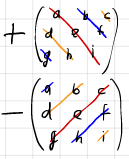
\includegraphics[width=.15\textwidth]{Dateien/00/14Sarrus.PNG}
\end{tabular}
\end{Satz}
\begin{Beispiel}
{Anwendung: Regel von Sarrus}
\begin{equation*}
    \det\Matrix{1&2&3\\4&5&0\\2&3&4}=1\cdot5\cdot4+2\cdot0\cdot2+4\cdot3\cdot3-4\cdot2\cdot4-1\cdot3\cdot0-2\cdot5\cdot3=20+36-32-30=-6
\end{equation*}
\end{Beispiel}
\begin{Satz}
{Rechenregeln}{Erlaubte Umformungen für Determinanten}
Beim Berechnen von Determinanten \underline{ändert sich nichts am Wert}, wenn wir
\begin{enumerate}
    \item Spalten vertauschen und dabei jeweils mit -1 multiplizieren:
    \blue{\begin{equation*}
        \det\Matrix{a&b&c\\d&e&f\\g&h&i}=-\det\Matrix{a&c&b\\d&f&e\\g&i&h}
    \end{equation*}}
    \item Vielfaches von Spalten zu anderen hinzuaddieren:
    \blue{\begin{equation*}
        \det\Matrix{a&b\\c&d}=\det\Matrix{a&b+2a\\c&d+2c}
    \end{equation*}}
    \item Die Matrix transponieren:
    \blue{\begin{equation*}
        \det A=\det\Matrix{a&b&c\\d&e&f\\g&h&i}=\det\Matrix{a&d&g\\b&e&h\\c&f&i}=\det A^T
    \end{equation*}}
\end{enumerate}
\blue{Aus der letzten Aussage ergibt sich, dass Zeilenumformungen genauso erlaubt sind wie Spaltenumformungen. Wir dürfen also quasi den Gauß-Algorithmus auf $A$ anwenden, nur dass wir Zeilen/Spalten nicht einfach vervielfachen dürfen und bei Vertauschungen aufpassen müssen.}
\end{Satz}
\begin{Satz}
{Rechenregel}{Determinanten mit Blockdreiecksmatrizen}
Die Determinante einer Blockdreiecksmatrix $E\in\Met(n+m,\mathbb{K})$, die sich aus den Matrizen $A\in\Met(n,\mathbb{K})$, $B\in\Met(n,m,\mathbb{K})$ und $D\in \Met(n,\mathbb{K})$ und der $m\times n$-Nullmatrix $\Vec{0}$ zusammensetzt, ist das Produkt der Determinanten von $A$ und $D$, d. h.
\begin{equation}
    \det\Matrix{A&B\\\Vec{0}&D}=\det A\cdot \det D.
\end{equation}
\end{Satz}
Aufgrund dieses Satzes reicht es auch, die Hauptdiagonalelemente miteinander zu multiplizieren, nachdem man erfolgreich den Quasi-Gaußalgorithmus\footnote{Wie gesagt, Achtung beim Vertauschen von Spalten/Zeilen und bei der Multiplikation mit Skalaren!} angewendet hat, d. h.
\begin{equation*}
    \det\Matrix{a_1& b &\cdots & c&d\\0&a_2&\cdots &e&f\\\vdots &  &\ddots & &\vdots\\0&0&\cdots &a_{n-1}&g\\0&0&\cdots &0&a_n}=\prod_{i=1}^na_i
\end{equation*}
\begin{Beispiel}
{Blockdreiecksmatrix (1/2)}
Wir können also ganz einfach die Determinante von folgender Monstermatrix berechnen:
\begin{equation*}
    \det\Matrix{1&2&3&4&5\\2&0&-2&4&6\\0&0&1&0&2\\0&0&2&1&0\\0&0&2&10&1}\overset{\footnote{Satz über Blockdreiecksmatrizen}}{=}\det\Matrix{1&2\\2&0}\det\Matrix{1&0&2\\2&1&0\\2&10&1}\overset{\footnote{Regel von Sarrus ergibt für die zweite Matrix $\det B=1+40+0-4-0-0=37$}}{=}(-4)37=-148.
\end{equation*}
\end{Beispiel}
\begin{Beispiel}
{Anwendung verschiedener Umformungen (2/2)}
Wir betrachten wieder die Matrix, die wir schon für die Regel von Sarrus kennengelernt hatten, und wollen auf verschiedene Weisen die Determinante bestimmen:\\
\begin{eqnarray*}
\det\Matrix{1&2&3\\4&5&0\\2&3&4}&\overset{\footnote{Transponieren}}{=}&\det\Matrix{1&4&2\\2&5&3\\3&0&4}\overset{\footnote{Erlaubte Umformung: $(II)- 2\cdot (I)$ und $(III)-3\cdot(I)$}}{=}\det\Matrix{1&4&2\\0&-3&-1\\0&-12&-2}\\
&\overset{\footnote{Satz zur Blockdreiecksmatrix}}{=}&\det(1)\det\Matrix{-3&-1\\-12&-2}\overset{\footnote{$\det (1)=1$, da es die $1\times 1$ Einheitsmatrix ist.\\Zudem nutzen wir die Linearität der Spalten, um die Faktoren $-3$ und $-1$ herauszuziehen}}{=}1(-3)(-1)\det\Matrix{1&1\\4&2}\\
&\overset{\footnote{Umformung: $(II)-4(I)$}}{=}&+3\Matrix{1&1\\0&-2}\overset{\footnote{Blockdreiecksmatrix}}{=}3\det(1)\det(-2)=-6
\end{eqnarray*}
Ein andere Möglichkeit wäre die Erzeugung der Stufenform:
\begin{eqnarray*}
\det\Matrix{1&2&3\\4&5&0\\2&3&4}&=&\det\Matrix{1&2&3\\0&-3&-12\\0&-1&-2}\overset{\footnote{Vertauschen zweier Zeilen, daher $(-1)$}}{=}-\det\Matrix{1&2&3\\0&-1&-2\\0&-3&-12}\\
&=&\det\Matrix{1&2&3\\0&-1&-2\\0&0&-6}=(-1)(-1)(-6)=-6.
\end{eqnarray*}
\end{Beispiel}

\subsubsection{Der Laplace'sche Entwicklungssatz}
Um den nächsten wichtigen Satz einzuführen, benötigen wir folgenden Begriff:
\begin{Def}
{Streichungsmatrix}
\begin{wrapfigure}{r}[0pt]{.35\textwidth}
 \vspace{-30pt}
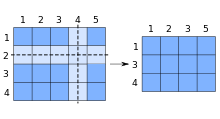
\includegraphics[width=.35\textwidth]{Dateien/01/01Submatrix_qtl1.svg.png}
 \vspace{-15pt}
\end{wrapfigure}
Für eine quadratische Matrix $A=(a_{kl})\in\Met(n,\mathbb{K})$ nennen wir $A_{ij}\in\Met(n-1,\mathbb{K})$ die ($i,j$)-te \red{Streichungsmatrix}\footnote{wobei $i,j\in\{1,...,n\}$. Dieser Begriff ist unter \href{https://de.wikipedia.org/wiki/Untermatrix}{Wikipedia} unter dem Namen 'Untermatrix' zu finden.}, die aus $A$ durch das Streichen der $i$-ten Zeile und $j$-ten Spalte entsteht.
\end{Def}
Durch den Laplace'schen Entwicklungssatz lässt sich die Berechnung der Determinante auf die Berechnung einiger 'kleinerer' Determinanten reduzieren.\\
Hierfür kann man eine Matrix $A$ nach der $i$-ten oder der $j$-ten Spalte \textit{entwickeln}:
\begin{Satz}{Satz}{Entwicklungssatz von Laplace}
Für die Determinante einer Matrix $A=(a_{kl})\in\Met(n,\mathbb{K})$ gilt
\begin{equation}
    \det A=\sum_{j=1}^n(-1)^{i+j}a_{ij}\det A_{ij}.
\end{equation}
\end{Satz}
Das sieht ziemlich wild aus, ist aber tatsächlich recht einfach:\\
Wir schnappen uns z.B. die erste Zeile und multiplizieren deren Einträge mit den Determinanten der Streichungsmatrizen und ggf. noch mit $(-1)$.
Wann ihr mit $(-1)$ multiplizieren müsst, könnt ihr euch nach folgendem Muster merken:
\begin{center}
    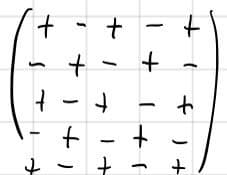
\includegraphics[width=.15\textwidth]{Dateien/01/01Laplacschema.jpg}
\end{center}
Es ist also immer alternierend.\\
\blue{\textbf{Hinweis}:\\
Es ist egal, nach welcher Zeile oder Spalte ihr entwickelt. Es lohnt sich häufig, gerade die Spalten/Zeilen zu wählen, die viele Nullen enthalten.}\\
Für das Beispiel, das wir auch im \textit{Determinanten}-Kapitel betrachtet hatten, sieht das dann so aus:
\begin{Beispiel}{Determinanten mit dem Entwicklungssatz berechnen}
Wir führen eine Entwicklung nach der ersten Zeile durch:
\begin{align*}
\det\Matrix{1&2&3\\4&5&0\\2&3&4}&=(-1)^{1+1}1\det\Matrix{5&0\\3&4}+(-1)^32\det\Matrix{4&0\\2&4}+3\det\Matrix{4&5\\2&3}\\
&=20-2\cdot16+3(12-10)=-12+6=-6.
\end{align*}
Alternativ können wir auch nach der dritten Spalte entwickeln:
\begin{align*}
\det\Matrix{1&2&3\\4&5&0\\2&3&4}&=(-1)^{1+3}3\det\Matrix{4&5\\2&3}+0+(-1)^{3+3}4\det\Matrix{1&2\\4&5}\\
&=3\cdot2+4(-3)=-6.
\end{align*}
\end{Beispiel}
Abschließend noch ein schönes Beispiel:
\begin{Beispiel}{Determinanten-Induktion}
\Zz{Für $n\in\mathbb{N}\setminus\{0\},\,a,b\in\mathbb{K}^n$ ist die Determinante einer Matrix $A$ der folgenden Gestalt durch
\begin{equation*}
    \det A=\det \Matrix{a_1&0&\cdots &\cdots&0&b_1\\
    0&\ddots&&&\iddots &0\\
    \vdots&&a_n&b_n&&\vdots\\
    \vdots&&b_n&a_n&&\vdots\\
    0&\iddots&&&\ddots &0\\
    b_1&0&\cdots &\cdots&0&a_1}=\prod_{k=1}^n(a_k^2-b_k^2)
\end{equation*}
gegeben.}
\Zb{Vollständige Induktion:\\
Induktionsanfang:\\
Für $n=1$ ist $\det A=\det\MatrixInline{a_1&b_1\\b_1&a_1}=a_1^2-b_1^2=\prod_{k=1}^n(a_k^2-b_k^2)$.\\
Es gelte die Induktionsvoraussetzung (siehe Aussage) für $n\geq 1$.\\
Induktionsschritt:\\
So folgt die Aussage für $n+1$, denn:
\begin{eqnarray*}
    \det A&=&\MatrixAbs{a_1&0&\cdots &\cdots&0&b_1\\
    0&\ddots&&&\iddots &0\\
    \vdots&&a_{n+1}&b_{n+1}&&\vdots\\
    \vdots&&b_{n+1}&a_{n+1}&&\vdots\\
    0&\iddots&&&\ddots &0\\
    b_1&0&\cdots &\cdots&0&a_1}\\
    &\overset{\footnote{Laplace-Entwicklung nach der $n+1$-ten Zeile}}{=}&a_{n+1}\MatrixAbs{a_1&0&\cdots &0&b_1\\
    0&\ddots&&\iddots &0\\
    \vdots&&a_{n+1}&&\vdots\\
    0&\iddots&&\ddots &0\\
    b_1&0&\cdots &0&a_1}-b_{n+1}\MatrixAbs{a_1&0&\cdots &0&b_1\\
    0&\ddots&&\iddots &0\\
    \vdots&&b_{n+1}&&\vdots\\
    0&\iddots&&\ddots &0\\
    b_1&0&\cdots &0&a_1}
\end{eqnarray*}
\begin{eqnarray*}
    &\overset{\footnote{Erneute Entwicklung nach der $n+1$-ten Zeile}}{=}&a_{n+1}^2\MatrixAbs{a_1&0&\cdots &\cdots&0&b_1\\
    0&\ddots&&&\iddots &0\\
    \vdots&&a_{n}&b_{n}&&\vdots\\
    \vdots&&b_{n}&a_{n}&&\vdots\\
    0&\iddots&&&\ddots &0\\
    b_1&0&\cdots &\cdots&0&a_1}-b_{n+1}^2\MatrixAbs{a_1&0&\cdots &\cdots&0&b_1\\
    0&\ddots&&&\iddots &0\\
    \vdots&&a_{n}&b_{n}&&\vdots\\
    \vdots&&b_{n}&a_{n}&&\vdots\\
    0&\iddots&&&\ddots &0\\
    b_1&0&\cdots &\cdots&0&a_1}\\
    &\overset{\footnote{Nutze die Induktionsvoraussetzung}}{=}&a_{n+1}^2\prod_{k=1}^n(a_k^2-b_k^2)-b_{n+1}^2\prod_{k=1}^n(a_k^2-b_k^2)\\
    &=&(a_{n+1}^2-b_{n+1}^2)\prod_{k=1}^n(a_k^2-b_k^2)\\
    &=&\prod_{k=1}^{n+1}(a_k^2-b_k^2)
\end{eqnarray*}}
\end{Beispiel}

\begin{Satz}
{Rechenregeln}{Zusammenfassung weiterer wichtiger Eigenschaften}
Wie wir gesehen hatten, gilt für $A, B, \mathds{1}_n\in\mathbb{N}$:
\begin{itemize}
    \item $\det(\mathds{1}_n)=1$
    \item $\det(A)=\det(A^T)$
    \item $\det(AB)=\det(A)\det(B)$
    \item $\det(A^{-1})=\det(A)^{-1}$ falls $\det (A)\neq0$.
\end{itemize}
\end{Satz}
\blue{\textbf{Tipp}:\\
Das Video \textbf{The Determinant} von 3Blue1Brown auf Youtube (unter \href{https://youtu.be/Ip3X9LOh2dk}{diesem Link} zu finden) erklärt sehr anschaulich die geometrische Bedeutung der Determinante als Maß für das Volumen der geometrischen Figur, auf die die Einheitsvektoren abgebildet werden.\\
Unserer Meinung nach bietet der Kanal generell sehr anschauliche Videos zu mathematischen Themen.}

\subsection{Zeit, umzukehren}
Wir betrachten nun einige Werkzeuge zum Invertieren von Matrizen. Dazu kurz nochmal ein Rückblick:
\begin{Wiederholung}{Lemma zur Bijektivität und Umkehrabbildung}\label{satz:BijektivitatUmkehrabbildung}
Eine Abbildung $f:A\rightarrow B$ ist \underline{genau dann bijektiv}, falls es eine Abbildung $g:B\to A$ gibt (diese nennen wir dann \red{Umkehrabbildung}), die die folgenden Relationen erfüllt:
\begin{equation}
    g\circ f=\text{Id}_A\,\wedge\, f\circ g=\text{Id}_B.\label{eq:Umkehrabbildung}
\end{equation}
\end{Wiederholung}
Wie wir schon festgestellt hatten, ist eine Matrix $A\in\Met(n,\mathbb{K})$ genau dann \red{invertierbar}, wenn $\det A\neq 0$.\\
Was bedeutet aber \textit{invertierbar}?
\begin{Wiederholung}{Inverse Matrix}
Ist $A$ invertierbar, so existiert eine \red{zu $A$ inverse Matrix $A^{-1}$}, sodass gilt:
\begin{equation}
    A\cdot A^{-1}=\mathds{1}_n\quad\tx{und}\quad A^{-1}\cdot A=\mathds{1}_n.
\end{equation}
\end{Wiederholung}
Falls $A$ die darstellende Matrix eines Endomorphismus ist, so ist dieser dann bijektiv und wir nennen ihn \red{Automorphismus}. Seht ihr die Parallelen zum Lemma zur Umkehrabbildung?\
\begin{Beispiel}{Inverse Matrix}
Sei $A=\Matrix{2&2\\3&4}$.\\
\Zz{Die Matrix $A^{-1}=\Matrix{2&-1\\-\frac{3}{2}&1}$ ist die zu $A$ inverse Matrix.}
\Zb{Es gilt 
\begin{equation*}
    A\cdot A^{-1}=\Matrix{2&2\\3&4}\Matrix{2&-1\\-\frac{3}{2}&1}=\Matrix{4-3&-2+2\\6-6&-3+4}=\Matrix{1&0\\0&1}=\mathds{1}_2
\end{equation*}
und analog andersherum.}
\end{Beispiel}

\begin{Wiederholung}{Inverse einer Determinante}
Für alle Gruppenhomomorphismen gilt $\phi(a^{-1})=\phi(a)^{-1}$. Somit gilt für alle\\
$A\in\GL(n,\mathbb{K})$:
\begin{equation}
    \det(A^{-1})=\det(A)^{-1}.
\end{equation}
Dies ist wohldefiniert, da $A\in\GL(n,\mathbb{K})$ per Definition bijektiv ist und somit eine Umkehrabbildung $A^{-1}$ besitzt und die Determinante nicht verschwindet.
\end{Wiederholung}
\begin{Wiederholung}
{Anwendung der Inversen Determinante}
Sei $A=\Matrix{2&2\\3&4}$. Die inverse Matrix ist (wie eben gesehen) $A^{-1}=\Matrix{2&-1\\-\frac{3}{2}&1}$.\\
Somit gilt:
\begin{align*}
    \det(A^{-1})&=2-(-1)(-3/2)=2-\frac{3}{2}=\frac{1}{2}\\
    \det(A)^{-1}&=(2\cdot 4-3\cdot 2)^{-1}=2^{-1}=\frac{1}{2}.
\end{align*}
\end{Wiederholung}
\begin{Def}
{Spezielle lineare Gruppe}
Wir bezeichnen die Untergruppe aller Automorphismen mit $\det A=1$ als \red{spezielle lineare Gruppe} und schreiben
\begin{equation}
    \SL=\Menge{A\in \GL(n,\mathbb{K})}{\det A=1}\subset \GL(n,\mathbb{K}).
\end{equation}
\end{Def}


\subsubsection{Invertieren mit dem Gauß-Verfahren}
Wie finden wir aber nun die inverse Matrix zu einer gegebenen Matrix $A$?
\begin{Satz}
{Rechenregel}{Invertieren einer Matrix mit Gauß}
Die erste Idee ist, dass wir ein Gleichungssystem umwandeln, indem wir mit $A^{-1}$ multiplizieren, d. h.
\begin{equation*}
    A\xvec=\Hat{\Vec{e}}_i\to \xvec=A^{-1}\Hat{\Vec{e}}_i.
\end{equation*}
Eine solche Überführung können wir durch den Gaußschen Algorithmus erreichen.\\
Um das für alle Spalten von $A^{-1}$ gleichzeitig zu machen, lösen wir also $(A\furdas\mathds{1}_n)\to(\mathds{1}_n\furdas A^{-1})$.
\end{Satz}
Das hört sich vielleicht komplizierter an, als es ist, daher hier ein Beispiel.
\begin{Beispiel}
{Invertieren einer Matrix mit Gauß}
Wir wollen die Matrix $A\in \GL(3,\mathbb{R}),\,A=\MatrixInline{1&2&3\\2&1&-1\\0&0&2}$ invertieren:
\begin{align*}
    (A\furdas\mathds{1}_3)&=\MatrixInvertieren{1&2&3\\2&1&-1\\0&0&2}{1&0&0\\0&1&0\\0&0&1}\overset{\tx{II}-2\tx{I},\, \tx{III }/2}{\longrightarrow}\MatrixInvertieren{1&2&3\\0&-3&-7\\0&0&1}{1&0&0\\-2&1&0\\0&0&1/2}\\
    \overset{\tx{I}-3\tx{III},\,\tx{II}+7\tx{III}}&{\longrightarrow}\MatrixInvertieren{1&2&0\\0&-3&0\\0&0&1}{1&0&-3/2\\-2&1&7/2\\0&0&1/2}\overset{\tx{II}/(-3)}{\longrightarrow}\MatrixInvertieren{1&2&0\\0&1&0\\0&0&1}{1&0&-3/2\\2/3&-1/3&-7/6\\0&0&1/2}\\
    \overset{\tx{I}-2\tx{II}}&{\longrightarrow}\MatrixInvertieren{1&0&0\\0&1&0\\0&0&1}{-1/3&2/3&5/6\\2/3&-1/3&-7/6\\0&0&1/2}=(\mathds{1}_3\furdas A^{-1}).
\end{align*}
Somit ist $A^{-1}=\frac{1}{6}\MatrixInline{-2&4&5\\4&-2&-7\\0&0&3}$ die zu $A$ inverse Matrix.\\
Wie können wir das testen?
\begin{itemize}
    \item \textbf{Überprüfe die Determinanten}:\\
    $\det(A^{-1})\overset{!}{=}(\det A)^{-1}$. Es ist
    \begin{eqnarray*}
        \det(A^{-1})&\overset{\footnote{Regel von Sarrus, Linearität}}{=}&\BracedIn{\frac{1}{6}}^3\BracedIn{(-2)(-2)3-4\cdot4\cdot3}=\frac{1}{36}\BracedIn{2-8}=-\frac{6}{36}=-\frac{1}{6}.\\
        \det A&=&1\cdot 1\cdot 2-2\cdot 2\cdot 2=2-8=-6\implies (\det A)^{-1}=-\frac{1}{6}.
    \end{eqnarray*}
    Leider ist dieses Kriterium nur notwendig, aber nicht hinreichend. Es kann aber als schneller Test dienen.
    \item \textbf{Stumpf rechnen}:\\
    Wir berechnen einfach
    \begin{equation*}
        A\cdot A^{-1}=\frac{1}{6}\Matrix{-2&4&5\\4&-2&-7\\0&0&3}\Matrix{1&2&3\\2&1&-1\\0&0&2}\overset{\footnote{Wir tun an dieser Stelle einfach mal so, als hätten wir das wirklich gerechnet ;)}}{=}\Matrix{1&0&0\\0&1&0\\0&0&1}.
    \end{equation*}
    Dieses Kriterium ist dann sowohl notwendig als auch hinreichend.
\end{itemize}
\end{Beispiel}

\subsubsection{Invertieren mit der Adjunkten}
Es gibt eine weitere, unintuitivere Möglichkeit, Matrizen zu invertieren. Hierfür benötigen wir den Begriff der adjunkten Matrix:
\begin{Def}
{Adjunkte Matrix}
Für die Matrix $A=(a_{ij})_{ij}\in\Met(n,\mathbb{K})$ definieren wir die \red{adjunkte Matrix} $\Tilde{A}=(\Tilde{a}_{ij})_{ij}$, die die folgenden Einträge hat:
\begin{equation*}
    \Tilde{a}_{ij}=(-1)^{i+j}\det A_{ji}=\det(\Vec{a}_1\ldots\Vec{a}_{i-1}\Vec{e}_j\Vec{a}_{i+1}\ldots a_n),
\end{equation*}
wobei $A_{ji}$ die $ji$-te Streichungsmatrix ist.
\end{Def}
Das sieht auf den ersten Blick erst mal ungewohnt aus, also betrachten wir es genauer:
\begin{Beispiel}
{Adjunkte einer $2\times 2$-Matrix (1/2)}
Sei $A=\MatrixInline{a&b\\c&d}$, so finden wir
\begin{equation*}
    \Tilde{a}_{11}=(-1)^2\det d,\quad \Tilde{a}_{12}=(-1)^3\det b,\quad \Tilde{a}_{21}=(-1)^3\det c,\quad \Tilde{a}_{22}=(-1)^4\det a. 
\end{equation*}
Somit ist $\Tilde{A}=\MatrixInline{d&-b\\-c&a}$.
\end{Beispiel}
\begin{Beispiel}
{Adjunkte einer $3\times 3$-Matrix (2/2)}
Sei $A=\MatrixInline{a&b&c\\d&e&f\\g&h&i}$, so finden wir
\begin{equation*}
    \Tilde{a}_{11}=(-1)^2\det \Matrix{e&f\\h&i},\quad \Tilde{a}_{12}\overset{\footnote{Streichungsmatrix 2. Zeile, 1. Spalte}}{=}(-1)^3\det \Matrix{b&c\\h&i},\quad \Tilde{a}_{13}=(-1)^4\det\Matrix{b&c\\e&f}
\end{equation*}
und so weiter...
\end{Beispiel}
\begin{Satz}
{Satz}{Zur adjunkten Matrix}
Für die adjunkte Matrix $\Tilde{A}$ zu $A\in \Met(n,\mathbb{K})$ gilt:
\begin{equation}
    A\cdot \Tilde{A}=\det A\mathds{1}_n\quad\tx{und}\quad \Tilde{A}\cdot A=\det A\mathds{1}_n.
\end{equation}
\end{Satz}
Wir sehen also, dass die Adjunkte quasi die Struktur der inversen Matrix hat, jedoch um einen Faktor $\det A$ daneben liegt.
\begin{Satz}
{Rechenregel}{Cramersche Regel zur Bestimmung der inversen Matrix}
Mithilfe der Adjunkten können wir aufgrund des vorhergehen Satzes also leicht die inverse Matrix einer invertierbaren Matrix $A\in\GL(n,\mathbb{K})$ bestimmen, denn es gilt
\begin{equation}
    \boxed{A^{-1}=\frac{1}{\det A}\Tilde{A}}.
\end{equation}
\end{Satz}
Der folgende Satz ist recht wichtig, es lohnt sich, ihn auswendig zu lernen:
\begin{Satz}
{Merksatz}{Inverse einer $2\times2$-Matrix}
Sehr häufig braucht man das Inverse einer $2\times2$-Matrix $A=\MatrixInline{a&b\\c&d}$.\\
Mithilfe der Adjunkten sehen wir:
\begin{equation}
    \label{eq:01InverseZweiKreuzZwei}A^{-1}=\frac{1}{\det A}\Tilde{A}=\frac{1}{ad-bc}\Matrix{d&-b\\-c&a}.
\end{equation}
\end{Satz}





\subsection{Exkurs: Volumen eines Parallelotops}\label{ssec:14AnhangParallelotop}
Hier wie versprochen noch ein schöner 'Appetithappen' zur Anwendung der Determinante

\begin{Beispiel}{Volumen eines Parallelotops}
Ein Parallelotop in einem $n$-dimensionalen Raum wird von $n$ Vektoren aufgespannt. Im Zweidimensionalen nennt man es
Parallelogramm, im Dreidimensionalen Parallelepiped.

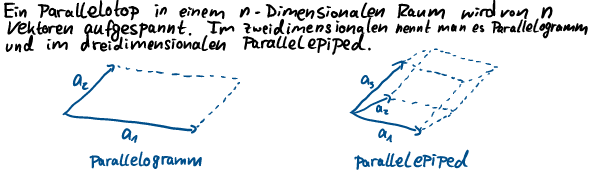
\includegraphics[width=0.8\textwidth]{Dateien/00/14Parallelotop1.png}

Die mathematische Definition lautet für $n$ Dimensionen:
\begin{equation}
    P(a_1, \ldots, a_n) = \{ x = \sum_{i=1}^n \lambda_i a_i | \lambda_1, \ldots, \lambda_n \in [0,1] \}
\end{equation}
Wir definieren für das Volumen:
\begin{equation}
    V(P(a_1, \ldots, a_n)) \eqqcolon V(a_1, \ldots, a_n) \eqqcolon V\overbrace{(a_1 \ldots a_n)}^{\substack{\text{Dies
    kann man als eine}\\ n\times n\text{ Matrix auffassen, mit den}\\\text{Vektoren }a_i\text{als Spalten}}}
\end{equation}
Es gibt hier noch eine kleine Feinheit: Sind die Vektoren $a_1, \ldots, a_n$ rechtshändig angeordnet, nennt man das
Parallelotop \red{positiv orientiert}, das Volumen ist somit positiv. Sind die Vektoren umgekehrt linkshändig
angeordnet, nennt man das Volumen \red{negativ orientiert}, das Volumen ist also negativ (ja, in der Mathematik darf man
das). Der Orientierungsbegriff wird euch noch oft wieder begegnen, hier hat er seinen Ursprung. Also unbedingt im
Hinterkopf behalten!

Für das Volumen eines Parallelotops stellen wir die folgenden Regeln fest:
\begin{enumerate}
    \item $V(a_1\ldots \mu a_i + \lambda b_i \ldots a_n) = \mu V(a_1 \ldots a_i \ldots a_n) + \lambda V(a_1 \ldots b_i
        \ldots a_n)$ mit $\mu, \lambda \in \mathds{R}$
    \item $a_i, a_j$ linear abhängig $\Rightarrow V(a_1 \ldots a_i \ldots a_j \ldots a_n) = 0$
    \item $V(e_1, \ldots, e_n) = 1$
\end{enumerate}
Die Begründung zeigen wir hier für $n=2$, sie sollte aber recht intuitiv auf beliebige Dimensionen erweiterbar sein.

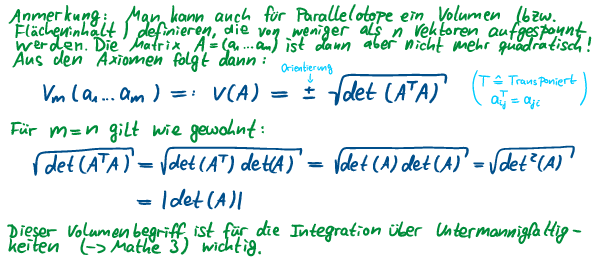
\includegraphics[width=0.8\textwidth]{Dateien/00/14Parallelotop2.png}

Ein strikter Beweis ist im Königsberger, Analysis 2 zu finden. Dort wird allerdings die Orientierung unterbunden, indem
der Betrag der Determinante genommen wird.\\
Damit sind wir auch schon beim Clou der ganzen Geschichte: Die Axiome
beider Methoden sind exakt gleich! Es gilt also:
\begin{equation}
    V(a_1\ldots a_n) = \det(a_1\ldots a_n)
\end{equation}

Anmerkung: Man kann auch für Parallelotope ein Volumen (bzw. Flächeninhalt) definieren, die von weniger als $n$ Vektoren
aufgespannt werden. Die Matrix $A=(a_1\ldots a_n)$ ist dann aber nicht mehr quadratisch! Aus den Axiomen folgt dann:
\begin{equation}
    V_m(a_1\ldots a_m) \eqqcolon V(A) = \overbrace{\pm}^{\text{Orientierung}} \sqrt{\det(A^TA)}
\end{equation}
Für $m=n$ gilt wie gewohnt:
\begin{gather}
    \sqrt{\det(A^TA)} = \sqrt{\det(A^T)\det(A)} = \sqrt{\det(A)\det(A)} = \sqrt{{\det}^2(A)} = |\det(A)| \\
    \text{mit } (a_{ij})^T = a_{ji} \text{ (transponiert)}\notag
\end{gather}
Dieser Volumenbegriff ist für die Integration über Untermannigfaltigkeiten ($\to$ Mathe 3) wichtig.
\end{Beispiel}


\subsection{Exkurs: Anwendung von Gruppen - Symmetrietransformationen}\label{ssec:ExkursSymTrafos}
Das Folgende ist nicht Teil der Mathevorlesung und vor allem für Interessierte gedacht. Ein paar Sachen werden euch dabei vielleicht in den Vorlesungen zur Quantenmechanik wiederbegegnen... \\
\begin{Beispiel}{Translationsgruppe (1/2)}
Schauen wir uns zunächst einmal die Translationsgruppe $T$ für eine Funktion \linebreak $f:\mathbb{R} \rightarrow \mathbb{R}$ an. Diese Gruppe besteht aus Elementen $t_{a}$, $a \in \mathbb{R}$, die wie folgt auf die Funktion wirken:
\begin{equation*}
    t_{a}f(x)=f(x+a).    
\end{equation*}
Sie verschieben also das Argument der Funktion um $a$. Es ist schnell zu erkennen, dass es ein inverses Element $t_{-a}$ und ein neutrales Element $t_{0}$ gibt, wenn wir die (assoziative) Verknüpfung wie folgt wählen:
\begin{equation*}
    t_{a}\cdot t_{b} = t_{a+b}.
\end{equation*}
Können wir nun eine spezielle Darstellung der Gruppenelemente finden? Aber klar! Dazu schauen wir uns eine infinitesimale Verschiebung $t_{da}$ an und erinnern an die Definition des Differenzenquotienten (denn wir hier mal auf Physikerart hinschreiben):
\begin{align*}
    \frac{df}{dx}=&\frac{f(x+da)-f(x)}{da} \\
    &\Rightarrow t_{da}f(x) = f(x+da) = f(x)+da \cdot \frac{df}{dx} = \big( 1 + da\frac{d}{dx} \big) f(x)
\end{align*}
Jetzt nutzen wir die Definition der Verknüpfung aus und erhalten für beliebige Transformationen:
\begin{align*}
    t_{a} = t_{\frac{a}{2}}\cdot t_{\frac{a}{2}} = ... &= \lim_{N \rightarrow \infty} \big( t_{\frac{a}{N}} \big)^{N} = \lim_{N \rightarrow \infty} \big( 1 + \frac{a}{N} \frac{d}{dx} \big)^{N} \\ 
    &= \exp{(a\frac{d}{dx})}
\end{align*}
Dabei haben wir benutzt, dass $a/N$ für große $N$ sehr klein und damit zu $da$ wird. Außerdem haben wir die Grenzwertdarstellung der Exponentialfunktion verwendet, die noch aus dem ersten Semester bekannt sein sollte. \\
Das interessante Ergebnis unserer kleinen Rechnung ist also:
\begin{equation*}
    t_{a}f(x)=\exp{(a\frac{d}{dx})}f(x) = f(x+a)
\end{equation*}
womit wir eine explizite Darstellung gefunden haben. Genau genommen nennt man das Argument der Exponentialfunktion ohne den Parameter $a$, also $d/dx$, die (Operator-)Darstellung der Translationsgruppe.
\end{Beispiel}
\begin{Beispiel}{Rotationsgruppe (2/2)}
Diese Art von Rechnung ist zum Beispiel in der Quantenmechanik sehr nützlich und kann auch auf Rotationen angewendet werden.\\
Die Rotationsgruppe\footnote{Wenn ihr Normen einführt, werdet ihr Lernen, dass diese Matrizen die Länge eines Vektors unverändert lassen und wegen $\det(R)=1$ keine Spiegelungen enthalten.} ist gegeben durch die spezielle orthogonale Gruppe $\text{SO}(N)$, wobei 
\begin{equation*}
    \text{SO}(N) := \Menge{R \in \Met(n,\mathbb{R})}{RR^{T}=R^{T}R=\mathds{1} \land \det(R) = 1}.
\end{equation*}
Der Einfachheit halber wollen wir hier nur Rotationen um die z-Achse in drei Dimensionen betrachten, die durch die wohlbekannte Matrix
\begin{equation*}
    R_{\theta} = \Matrix{\cos(\theta) & -\sin(\theta) & 0 \\ \sin(\theta) & \cos(\theta) & 0 \\ 0 & 0 & 1}
\end{equation*}
gegeben sind.\\
Eine Rotation $r_{\theta}$ einer Funktion $f:\mathbb{R}^{3} \rightarrow \mathbb{R}$ ist dann gegeben durch:
\begin{equation*}
    r_{\theta}f(v) = f(R_{\theta} v).
\end{equation*}
Diese Transformationen $r_{\theta}$ bilden aus denselben Gründen wie bei den Translationen eine Gruppe. \\
Können wir auch hier wieder eine explizite Darstellung finden? Aber natürlich! Dazu schauen wir uns abermals ein infinitesimale Transformation an und beachten dafür die Kleinwinkelnäherung $\sin(d\theta)=d\theta$ und $\cos(d\theta)=1$:
\begin{equation*}
    R_{d\theta}=\Matrix{1 & -d\theta & 0 \\ d\theta & 1 & 0 \\ 0 & 0 & 1}.
\end{equation*}
Daraus folgt:
\begin{equation*}
    r_{d\theta}f(v) = f(R_{d\theta}v) = f(x-yd\theta, y+xd\theta, z)
\end{equation*}
Jetzt packen wir den Zauberstab aus und spielen ein wenig mit den Differentialen herum, aber versprochen, es funktioniert! Im Differenzenquotienten packen wir erstmal einfach ein konstantes $y$ und $x$ hinzu, was uns ja keiner verbietet ($yd\theta$ ist ja immernoch sehr klein):
\begin{align*}
    \frac{df}{dx}&=\frac{f(x+(-yd\theta),y,z)-f(x,y,z)}{-yd\theta} \Leftrightarrow f(x-yd\theta,y,z)=(1-yd\theta\frac{d}{dx})f(x,y,z) \\
    \frac{df}{dy}&=\frac{f(x,y+xd\theta,z)-f(x,y,z)}{xd\theta} \Leftrightarrow f(x,y+xd\theta,z) = (1+xd\theta\frac{d}{dx})f(x,y,z)
\end{align*}
Daraus folgt, wenn wir annehmen, dass $d\theta^{2}$ sehr klein und somit vernachlässigbar ist:
\begin{align*}
    f(x-yd\theta,&y+xd\theta,z) = (1-yd\theta\frac{d}{dx})f(x,y+xd\theta,z)\\ &= (1-yd\theta\frac{d}{dx})(1+xd\theta\frac{d}{dx})f(x,y,z) = (1+xd\theta\frac{d}{dx}-yd\theta\frac{d}{dx})f(x,y,z).
\end{align*}
Wir haben also für die infinitesimale Rotation gefunden:
\begin{equation*}
    r_{d\theta}f(v)=(1+d\theta(x\frac{d}{dx}-y\frac{d}{dx}))f(v).
\end{equation*}
Das sieht doch schon mal richtig gut aus! Tatsächlich können wir hier den gleichen Trick wie bei der Translationsgruppe benutzen, um diese Vorschrift zu verallgemeinern:
\begin{align*}
    r_{\theta}f(v) = (r_{\frac{\theta}{2}})^{2}f(v)&=...=\lim_{N\rightarrow\infty}(r_{\frac{\theta}{N}})^{N}f(v)=\lim_{N\rightarrow\infty}(1+\frac{\theta}{N}(x\frac{d}{dx}-y\frac{d}{dy}))^{N}f(v)\\ &=\exp{(\theta(x\frac{d}{dy}-y\frac{d}{dx})}f(v) =: \exp{(\theta L)}f(v)
\end{align*}
Wir haben also tatsächlich eine (Operator-)Darstellung der Rotationsgruppe gefunden! Sie lautet:
\begin{equation*}
    L:=x\frac{d}{dy}-y\frac{d}{dx}.
\end{equation*}
\end{Beispiel}
Wir hoffen, dass diese doch etwas verschwurbelte Rechnung einigermaßen verständlich war. Sollte sie zu Verwirrung geführt haben, vergesst einfach die letzten beiden Seiten und konzentriert euch auf den wesentlichen Stoff! Vielleicht hat es ja trotzdem bei dem/der ein oder anderen, der/die auch schon Quantenmechanik (Physik 3) gehört und $L$ als den berühmten Drehimpulsoperator (oder besser gesagt seine z-Komponente) erkannt hat, zu einem Aha-Erlebnis geführt. Es sind unserer Meinung nach einfach zwei sehr schöne Beispiele für die Verwendung von Gruppen.

\Tipps{1}{
\begin{enumerate}
    \item Die Formulierung ist vielleicht etwas ungewohnt, aber fasst einfach die Polynome als Vektor auf und sucht euch zunächst ein Beispiel.\\
    Auf was wird z. B. das Polynom $P(x)=5+7x-3x^3=\MatrixInline{5\\7\\0\\-3}$ durch die Ableitung abgebildet?\\
    Dann müsst ihr euch überlegen, wie ihr diese lineare Abbildung mithilfe einer Matrix aufschreiben könnt.\\
    Alternativ könnt ihr auch ganz klassisch schauen, was die Ableitung mit den Basisvektoren der Basis $(1,x,x^2,x^3)$ macht, und wie ihr das Ergebnis durch diese wieder darstellen könnt. Spaltenweise aufgeschrieben ergibt das dann eure Matrix.\\
    Spur und Determinante sollten ein Kinderspiel sein.
    \item Auch bei dieser Aufgabe handelt es sich um relativ kurze Rechnungen. Bei a.) erinnert euch einfach daran, wie Linearität definiert ist. Auch bei b.) schaut euch an, was für Matrizen gelten muss, die im Kern von $\varphi$ liegen und welche Bedingungen daraus für die Matrixelemente folgen. In c.) müsst ihr das Bild auf Symmetrie untersuchen und euch überlegen, wie man beliebige symmetrische Matrizen so zerlegen kann, dass sie ein Bild von $\varphi$ sind. Für d.) schaut euch nochmal die Körperaxiome an.
    \item Determinanten zu berechnen ist eines der wichtigsten Werkzeuge dieses Semesters, also setzt euch in Ruhe daran und geht alle Sätze durch, die ihr dafür nutzen könntet - Eventuell ist es sogar sinnvoll, die Determinanten mit verschiedenen Wegen zu berechnen.\\
    Nützlich sind natürlich quasi-Gauß'sche Umformungen, der Satz über Blockdreiecksmatrizen, die Cramer'sche Regel, die Regel von Sarrus und der Laplace'sche Entwicklungssatz die gängigen Mittel.
    \item  
    \begin{enumerate}
        \item Hier hilft es, die Linearität der Determinante auszunutzen - welche Spalte bietet sich dafür an? Denkt dann an den Gauß-Algorithmus.\\
        Ihr solltet bei einem Ausdruck der Form
        \begin{equation*}
            \det A= \prod_{i=1}^n a_i+\sum_{k=1}^nb_k\prod_{j\neq k}^n c_j
        \end{equation*}
        kommen.
        \item Wir sehen leider nicht, wie man das mit Induktion macht, wir haben das mithilfe eines direkten Beweises und Aufgabe 3a) gemacht. Auch hier gilt wieder: Linearität ausnutzen!\\
        Weiterer Tipp (der in ähnlicher Form vielleicht nützlich ist):
        \begin{equation*}
            \det\Matrix{a_1&a_2&a_3\\a_1&a_2&a_3\\a_1&a_2&a_3}=\prod_{i=1}^3a_i\det\Matrix{1&1&1\\1&1&1\\1&1&1}
        \end{equation*}
    \end{enumerate}
\end{enumerate}
}



\section[Eigenzeugs]{Eigenwerte, Eigenvektoren und Eigenräume}
\Einleitung{Zunächst wagen uns noch einmal an Äquivalenzrelationen heran und schauen, wie wir damit Automorphismen eine Orientierung verleihen können.\\
Danach machen wir den ersten Schritt zur Diagonalisierung von Endomorphismen. Dies ist der Prozess, für einen Endomorphismus\footnote{der bestimmte Eigenschaften haben muss} $F\in \End(V)$ die Basis $B$ des zugrunde liegenden Vektorraums $V$ geschickt so zu wählen, dass die darstellende Matrix $M_B(F)$ nur noch Einträge auf der Diagonalen hat. Dazu müssen wir zunächst Begriffe wie Eigenwerte, Eigenvektoren und Eigenräume verstehen. Eigenvektoren sind Vektoren, die auf ein Vielfaches ihrer selbst\footnote{dieses Vielfache ist dann der Eigenwert} abgebildet werden, d. h. die Gleichung $A\Vec{v}=\lambda \Vec{v}$ erfüllen.\\
Ein wichtiges Werkzeug ist dabei das charakteristische Polynom, das wir auf endlichdimensionalen Vektorräumen verwenden können und das die Determinante zur Hilfe nimmt.}

\subsubsection{Basiswechsel und Orientierung von Automorphismen}
Die Mühe mit den Äquivalenzklassen haben wir uns vor allem gemacht, um gleich orientierte Basen als äquivalent einzustufen. Aber der Reihe nach:
\begin{Def}
{Basiswechsel}
Da die Basis von Vektorräumen nicht eindeutig ist, können wir lineare Abbildungen definieren, die von der einen in die andere Basis wechseln. Damit keine Information verloren geht, müssen diese bijektiv sein.\footnote{Wir betrachten also Automorphismen.}\\
Der \red{Basiswechsel} zwischen Basen $B$ und $B'$ von $V$ ist nun als folgende lineare Abbildung definiert:
\begin{equation}
    F:V\to V,\quad F(v)=\phi_{B'}(\phi_B^{-1}(v)),
\end{equation}
wobei $\phi_{B'}$ und $\phi_B$ lineare Abbildungen sind, für die die jeweiligen Basisvektoren spaltenweise in eine Matrix geschrieben werden.
\end{Def}
\begin{Beispiel}
{Basiswechsel im $\mathbb{R}^2$}
Wir betrachten $V=\mathbb{R}^2$ mit den Basen $B=\left\{\MatrixInline{1\\1},\MatrixInline{2\\0}\right\}$ und $B'=\left\{\MatrixInline{0\\2},\MatrixInline{1\\4}\right\}$.
Hier ist $\phi_B=\Matrix{1&2\\1&0}$ und $\phi_{B'}=\Matrix{0&1\\2&4}$.\footnote{denn z. B. gilt $\phi_B(\Vec{e}_1)=\Matrix{1\\1}\,\checkmark$}\\
Da wir von $B$ nach $B'$ wollen, müssen wir nun $\phi_B^{-1}$ bestimmen, also die inverse Matrix zu $\phi_B$ finden. Dafür nutzen wir die \href{https://de.wikipedia.org/wiki/Cramersche_Regel}{Cramersche Regel}:
\begin{equation*}
\phi_B^{-1}=\frac{1}{\det \phi_B}\Matrix{0&-2\\-1&1}\overset{\footnote{Es ist $\det \phi_B=-2$.}}{=}\frac{1}{2}\Matrix{0&2\\1&-1}.
\end{equation*}
Somit ist der Basiswechsel (bzw. dessen darst. Matrix) gegeben durch 
\begin{equation*}
F=\phi_{B'}\circ\phi_B^{-1}=\frac{1}{2}\Matrix{0&1\\2&4}\Matrix{0&2\\1&-1}=\Matrix{1&-1\\4&0}.
\end{equation*}
\end{Beispiel}



\begin{Def}
{Orientierung}
Wir nennen zwei Basen eines reellen Vektorraums \red{gleich orientiert}, wenn der Basiswechsel $F=\phi_{B'}\phi_B^{-1}: V\to V$ eine \underline{positive Determinante} hat.\\
\blue{Anmerkung: Da es sich um eine bijektive Abbildung handeln muss, ist $\det F$ niemals 0.}
\end{Def}

\begin{Beispiel}
{Orientierung des obigen Basiswechsels}
Für den Basiswechsel $B=\left\{\MatrixInline{1\\1},\MatrixInline{2\\0}\right\}\to B'=\left\{\MatrixInline{0\\2},\MatrixInline{1\\4}\right\}$ bedeutet das, dass die Basen gleich orientiert sind, denn $\det F= 1\cdot 0-(-1)4=4$.
\end{Beispiel}

\begin{Satz}{Folgerung}{Die Orientierung ist eine Äquivalenzrelation}
Wir können $B\sim B'\iff $ \textit{$B$ und $B'$ sind gleich orientiert} als Äquivalenzrelation auffassen.\\
Dann definiert jede Basis eine Äquivalenzklasse $[B]$ bzw. eine Orientierung. Es gibt genau zwei Orientierungen.
\end{Satz}

\begin{Def}
{Positive Orientierung}
Wir nennen $B$\footnote{Basis von $V$ mit $\dim V=n$.} \red{positiv orientiert}, wenn sie dieselbe Orientierung wie die kanonische Basis $B_e=\{\Vec{e}_1,\ldots,\Vec{e}_n\}$ hat. Andernfalls nennen wir $B$ \red{negativ orientiert}.
\end{Def}
Dieses Konzept kennt ihr bestimmt schon aus dem $\mathbb{R}^3$: Die kanonische Basis und alle positiv orientierten Basen könnt ihr mit der \textit{Rechte-Hand-Regel} nachvollziehen, alle anderen mit der linken Hand.
\begin{Beispiel}{Orientierung zweier Basen}
\begin{wrapfigure}{r}[0pt]{.35\textwidth}
 \vspace{-15pt}
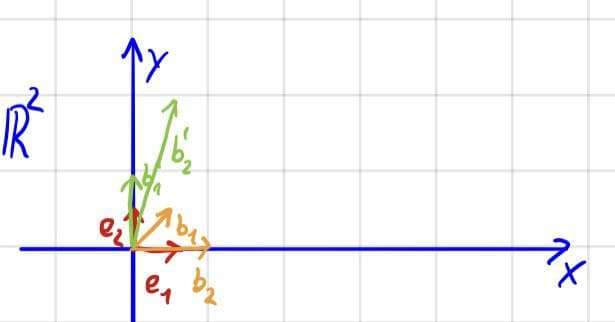
\includegraphics[width=.35\textwidth]{Dateien/01/01Basiswechsel.jpg}
 \vspace{-15pt}
\end{wrapfigure}
Der Basiswechsel von $B_e\to B$ ist sehr einfach, da $\phi_{B_e}^{-1}=\phi_{B_e}=\mathds{1}_n$. Also müsst ihr für den Basiswechsel von $B_e\to B$  eigentlich nur die Determinante von $\phi_B$ berechnen.\\
Wir betrachten wieder $B=\left\{\MatrixInline{1\\1},\MatrixInline{2\\0}\right\}$.\\
Hier ist $\det(\phi_B\circ\phi_{B_e}^{-1})=\det\phi_B=\det\MatrixInline{1&2\\1&0}=-2$.\\
Somit ist $B$ nicht gleich wie die kanonische Basis, also negativ orientiert.\\
Aufgrund der vorigen Feststellung, weil $B\sim B'$, ist auch $B'$ negativ orientiert. Alternativ ergibt das auch der folgende Test:\\ $\det(\phi_{B'}\circ\phi_{B_e}^{-1})=-2$.
\end{Beispiel}

\begin{Def}{Orientierung eines Automorphismus}
Abgesehen von Basiswechseln nennen wir allgemein Automorphismen $F\in \GL(V)$ \red{orientierungserhaltend}, wenn $\det F>0$.\\
Analog nennen wir $F$ \red{orientierungsumkehrend}, wenn $\det F<0$.
\end{Def}

%%%%%%%%%%%%%%%%%%%%%%%%%%%%%%%%%%%%%%
\subsection{Mathematische Eigenartigkeiten - Eigenwerte und Eigenvektoren}
\begin{Def}
{Eigenwert und Eigenvektor}
Wird ein Vektor $\Vec{v}$\footnote{der nicht der Nullvektor ist!} durch einen Endomorphismus $F\in\End(V)$ auf ein Vielfaches $\lambda$ seiner selbst abgebildet, so nennen wir ihn \red{Eigenvektor} von $F$. Der Skalierungsfaktor $\lambda$ ist der zugehörige \red{Eigenwert}.\\
Anders geschrieben: $\Vec{v}$ erfüllt die \underline{Eigenwertgleichung}
\begin{equation}
\boxed{F(\Vec{v})=\lambda \Vec{v}}, \quad \Vec{0}\neq \Vec{v}\in V,\quad \lambda \in \mathbb{K}.
\end{equation}
\blue{Zu einem Eigenwert kann es verschiedene Eigenvektoren geben!}
\end{Def}

\begin{Def}
{Eigenraum}
Das lineare Erzeugnis aus allen Eigenvektoren zu einem gegebenen Eigenwert $\lambda$ nennen wir \red{Eigenraum} zum Eigenwert $\lambda$. Dieser ist stets ein Unterraum von $V$, wir schreiben
\begin{equation}
V_\lambda=\Menge{\Vec{v}\in V}{F(\Vec{v})=\lambda \Vec{v}}=\Span{\Vec{v}\in V}{\Vec{v} \tx{ ist Eigenvektor zu } \lambda}.
\end{equation}
\end{Def}

Wir schauen uns gleich die geometrische Bedeutung dieser Definitionen an, doch vorher ein paar Beispiele und Rechenregeln:
\begin{Beispiel}{Eigenzeugs im $\mathbb{R}^2$}
Betrachte $V=\mathbb{R}^2,\, F:=\MatrixInline{0&1\\1&0}\in \End(V)$.\\
Die Eigenwertgleichung ergibt dann:
\begin{equation*}
F(\Vec{v})=\lambda \Vec{v}\iff \Matrix{0&1\\1&0}\Matrix{x\\y}=\Matrix{\lambda x\\\lambda y}\iff y =\lambda x,\, x=\lambda y\implies y=\lambda^2 y\implies \lambda=\pm 1.
\end{equation*}
Die Eigenwerte sind also $\lambda=\pm 1$.\\
Für $\lambda_1=+1$ gilt $y=x$, also ist z. B. $\Vec{v}=\MatrixInline{1\\1}$ ein Eigenvektor zu $\lambda_1$.\\
Für $\lambda_2=-1$ gilt $y=-x$, also ist z. B. $\Vec{v}=\MatrixInline{-1\\1}$ ein Eigenvektor zu $\lambda_2$.\\
Die Eigenräume sind dann $V_{\lambda_1}=\Spann{\MatrixInline{1\\1}}$ und $V_{\lambda_2}=\Spann{\MatrixInline{-1\\1}}$\\
Es gibt nicht mehr Eigenwerte, da die Summe der Dimensionen der Eigenräume (hier $1+1=2$) stets kleiner gleich $\dim V$ ist (dazu später mehr).
\end{Beispiel}

\subsubsection{Das charakteristische Polynom}
\blue{\textbf{Motivation}:\\
Wir lernen nun ein wichtiges Werkzeug zur Bestimmung von Eigenwerten auf \textbf{endlich\-dim\-ension\-al\-en} Vektorräumen kennen:\\
\textbf{Das charakteristische Polynom}.\\
Wie sieht es aus? Und woher kommt das? Wir betrachten eine kurze Herleitung und gehen dafür von der bekannten Eigenwertgleichung aus:
\begin{alignat*}{2}
A\Vec{v}&=\lambda \Vec{v}&\furdas\tx{Wir formen nun einfach um: Es ist $\Vec{w}=\mathds{1}_n \Vec{w}\quad\forall \Vec{w}\in V$.}\\
\iff A\Vec{v} &=\mathds{1}_n(\lambda \Vec{v})&\furdas-\mathds{1}_n(\lambda \Vec{v}) \tx{ und Assoziativität: }\mathds{1}_n(\lambda \Vec{v})=(\mathds{1}_n\lambda)\Vec{v}.\\
\iff A\Vec{v}-\mathds{1}_n\lambda \Vec{v}&=\Vec{0}&\furdas \tx{Klammere $\Vec{v}$ aus. Zudem ist $\mathds{1}_n\lambda=\lambda\mathds{1}_n$, weil $\lambda$ ein Skalar ist.}\\
\iff (A-\lambda\mathds{1}_n)\Vec{v}&=\Vec{0}&\furdas\tx{Diese Gleichung kann nur erfüllt sein, wenn $\det(A-\lambda\mathds{1}_n)=0$ ist.}\\
\implies \det(A-\lambda\mathds{1}_n)&=0&\furdas \tx{Dies ist nun unser Werkzeug zum Finden von Eigenwerten.}
\end{alignat*}}
\begin{Def}{Charakteristisches Polynom}
Für $V$ mit $\dim V=n<\infty$ definieren wir für Endomorphismen $F\in \End(V)$ das \red{charakteristische Polynom} $P_F(\lambda)$ mit
\begin{equation}
P_F:\mathbb{K}\to\mathbb{K},\quad\boxed{P_F(\lambda)=\det(F-\lambda\Id)=\det(A-\lambda\mathds{1}_n)}
\end{equation}
wobei $A$ die darstellende Matrix von $F$ bzgl. einer beliebigen Basis von $V$ sei.
\end{Def}
\begin{Satz}{Satz}{Eigenwerte sind Nullstellen des charakteristischen Polynoms}
Die Eigenwerte von $F$ sind genau die Nullstellen des charakteristischen Polynoms, d. h.
\begin{equation}
\boxed{\det(A-\lambda\mathds{1}_n)=0}\impliedby \lambda\tx{ ist Eigenwert von }F.
\end{equation}
\end{Satz}
\begin{Beispiel}{Bestimmung von Eigenwerten}
Betrachte $F:V\to V$ mit der darst. Matrix $A=\MatrixInline{2&1\\3&0}$ bzgl. der kanonischen Basis. Diese hat die Eigenwerte $\lambda_1=-1$ und $\lambda_2=3$, denn
\begin{align*}
P_F(\lambda)&=\det(A-\lambda\mathds{1}_2)=\det\Matrix{2-\lambda&1\\3&-\lambda}=-2\lambda+\lambda^2-3\overset{!}{=}0\\
\overset{p-q}{\iff}\lambda_{1,2}&=-\frac{-2}{2}\pm\sqrt{1-(-3)}=1\pm 2.
\end{align*}
Nun können wir auch die Eigenvektoren bestimmen.\\
Dafür müssen wir das Gleichungssystem $A\Vec{v}=\lambda_i\Vec{v}$ lösen.\\
\begin{eqnarray*}
\lambda_1:\quad \Matrix{2&1\\3&0}\Matrix{x\\y}&=&-1\Matrix{x\\y}\overset{\footnote{Diesen Schritt würde ich immer empfehlen}}{\iff} \Matrix{3&1\\3&1}\Matrix{x\\y}=\Matrix{0\\0}\\
\overset{\footnote{Gauß-Schreibweise}}{\iff}\MatrixInvertieren{3&1\\3&1}{0\\0}&\overset{\tx{II}-\tx{I}}{\longrightarrow}&\MatrixInvertieren{3&1\\0&0}{0\\0}\implies y=t\in\mathbb{R}\tx{ bel.}\\
\iff 3x&=&-y\iff x=-\frac{t}{3}\\
\tx{Wähle $t=3$: }\implies \Vec{v}&=&\Matrix{-1\\3} \tx{ ist Eigenvektor.}\\
\tx{Der Eigenraum ist dann } V_{\lambda_1}&=&\Spann{\Matrix{-1\\3}}.\\
\lambda_2:\quad \Matrix{2&1\\3&0}\Matrix{x\\y}&=&3\Matrix{x\\y}\\
\overset{\footnote{Gauß-Schreibweise}}{\iff}\MatrixInvertieren{-1&1\\3&-3}{0\\0}&\overset{\tx{II}+3\tx{I}}{\longrightarrow}&\MatrixInvertieren{-1&1\\0&0}{0\\0}\implies y=t\in\mathbb{R}\tx{ bel.}\\
\iff -x&=&-y\iff x=t\\
\tx{Wähle $t=1$: }\implies \Vec{v}&=&\Matrix{1\\1} \tx{ ist Eigenvektor.}\\
\tx{Der Eigenraum ist dann } V_{\lambda_2}&=&\Spann{\Matrix{1\\1}}
\end{eqnarray*}
\end{Beispiel}

\begin{Def}
{Multiplizität der Nullstellen}
Ganz allgemein können wir jedes Polynom auch als Produkt seiner Nullstellen\footnote{bzw. $(x-x_0)$ etc.} und einem nicht-Null werdenden Rest schreiben.\\
Betrachten wir nur eine bestimmte Nullstelle, so können wir diese aus dem Rest \textit{herausziehen}:
\begin{equation*}
P(\lambda)=(\lambda-\lambda_i)^m\cdot Q(\lambda),
\end{equation*}
wobei $\lambda_i$ die Nullstelle und $Q(\lambda)$ der Rest (ebenfalls ein Polynom), für den $Q(\lambda_i)\neq 0$ gilt, sind.\\
Wir nennen die Potenz $m$ die \red{Vielfachheit} der Nullstelle $\lambda_i$.
\end{Def}

\begin{Beispiel}{Vielfachheit eines Polynoms}
Wir betrachten als Beispiel
\begin{equation*}
P(\lambda)=(\lambda-5)^3(\lambda+2)27(\lambda^2+1)
\end{equation*}
Hier hat $\lambda_1=5$ die Vielfachheit 3 und $\lambda_2=-2$ die Vielfachheit 1. Es gibt keine weitere Nullstelle.
\end{Beispiel}

\begin{Def}
{Algebraische Vielfachheit}
Im Zusammenhang mit dem charakteristischen Polynom von $F\in\End(V)$ nennen wir die Vielfachheit der Nullstelle $\lambda_i$ des char. Polynoms, die ja mit dem Eigenwert $\lambda_i$ korrespondiert, die \red{algebraische Vielfachheit $m_{\lambda_i}$} von $\lambda_i$.
\end{Def}

\begin{Def}
{Geometrische Vielfachheit}
Dem gegenüber steht die \red{geometrische Vielfachheit $n_{\lambda_i}$} des Eigenwertes $\lambda_i$, welche als Dimension des zu $\lambda_i$ gehörigen Eigenraumes\footnote{also die Anzahl der zum Eigenwert gehörigen linear unabhängigen Eigenvektoren.} definiert ist, d. h. $n_{\lambda_i}=\dim V_{\lambda_i}$.
\end{Def}

\begin{Satz}{Satz}{Beschränkung der Vielfachheiten}
Während die Summe aller algebraischen Vielfachheiten durch $\dim V=\grad P_F(\lambda)=n$ beschränkt ist, ist für jeden Eigenwert $\lambda_i$ die geometrische durch die algebraische Vielfachheit beschränkt, d. h.
\begin{equation}
\boxed{n_{\lambda_i}\leq m_{\lambda_i}}\quad \tx{und }\sum_{i=1}^km_{\lambda_i}\leq n=\dim V\tx{ mit $k$ der Anzahl der Eigenwerte.}
\end{equation}
\end{Satz}

\begin{Satz}{Satz}{Eigenvektoren sind linear unabhängig}
Die Familie der Eigenvektoren $(\Vec{v}_i)_{i=1...k}$ zu paarweise verschiedenen Eigenwerten ist linear unabhängig.\\
Wir sehen also:\\
Wenn die Summe der geometrischen Vielfachheiten $\sum_{i=1}^k n_{\lambda_i}=n=\dim V$ ist, gibt es also $n$ linear unabhängige Eigenvektoren. Diese bilden wiederum eine Basis von $V$, es ist $V=V_{\lambda_1}\oplus V_{\lambda_2}\oplus\ldots\oplus V_{\lambda_k}$, der Vektorraum wird in diesem Fall also durch die Eigenvektoren aufgespannt und ist die direkte Summe der Eigenräume!\\
Wir werden sehen, dass diese Basis spezielle Eigenschaften hat.
\end{Satz}

\begin{Beispiel}{Eigenwerte und Eigenräume}
Wir berechnen die Eigenwerte und Eigenräume zum Endomorphismus
\begin{equation*}
F: V\to V,\quad A_F=\Matrix{3&4&-3\\2&7&-4\\3&9&-5}.
\end{equation*}
Das charakteristische Polynom ist mit der Regel von Sarrus \eqref{eq:Sarrusregel}
\begin{align*}
P_F(\lambda)&=\det(A-\lambda\mathds{1}_n)\\
&=(3-\lambda)(7-\lambda)(-5-\lambda)+3(-4)4+2\cdot 9(-3)-2\cdot 4(-5-\lambda)\\
&\quad-(3-\lambda)9(-4)-3(-3)(7-\lambda)\\
&=-\lambda^3+5\lambda^2-8\lambda+4\overset{!}{=}0.
\end{align*}
Wir erraten die erste Nullstelle, $\lambda_1=1$.\\
Eine Polynomdivision ergibt $P_F(\lambda)/(\lambda-1)=-(\lambda-2)^2$.\\
Also ist $\lambda_2=2$ und wir können schreiben
\begin{equation*}
P_F(\lambda)=-(\lambda-1)^1(\lambda-2)^2\implies m_{\lambda_1}=1,\,m_{\lambda_2}=2.
\end{equation*}
\begin{wrapfigure}{r}[0pt]{.35\textwidth}
 \vspace{-15pt}
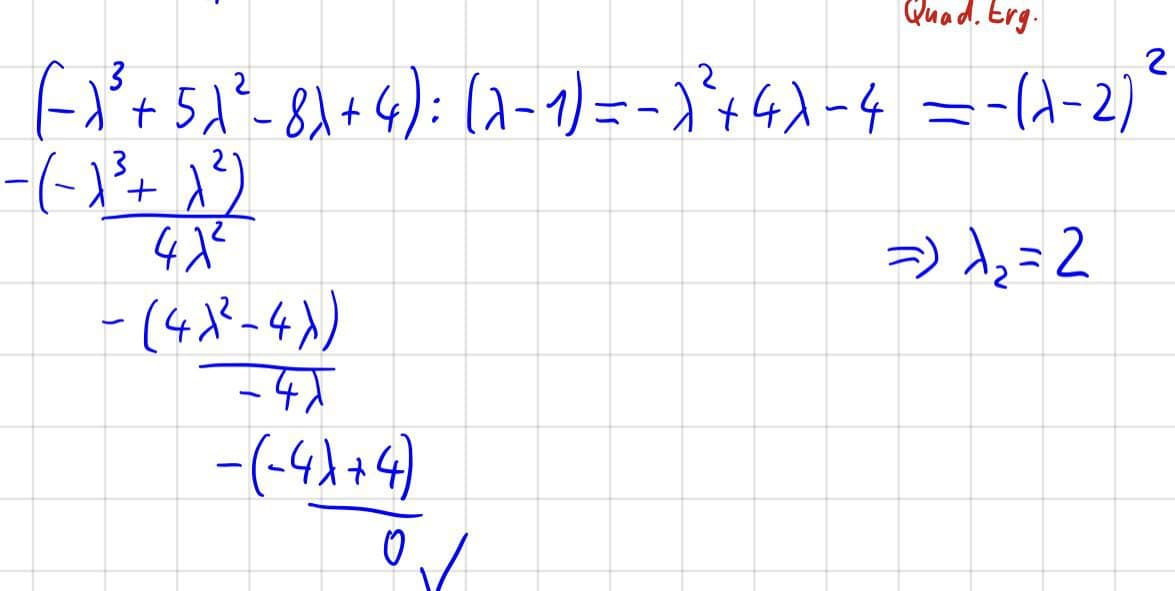
\includegraphics[width=.35\textwidth]{Dateien/01/01PolDiv.jpg}
 \vspace{-15pt}
\end{wrapfigure}
Wir bestimmen die Eigenvektoren und ziehen dafür direkt $\lambda_i$ auf der Hauptdiagonalen ab:
\begin{align*}
\lambda_1:\quad &\MatrixInvertieren{2&4&-3\\2&6&-4\\3&9&-6}{0\\0\\0}\overset{\frac{2}{3}\tx{III}}{\longrightarrow}\MatrixInvertieren{2&4&-3\\2&6&-4\\2&6&-4}{0\\0\\0}\\
&\overset{\tx{III}-\tx{II},\,\tx{II}-\tx{I}}{\longrightarrow}\MatrixInvertieren{2&4&-3\\0&2&-1\\0&0&0}{0\\0\\0}\implies z=t\in\mathbb{R}\tx{ bel.}\\
&\implies 2y=z\iff y=\frac{t}{2}\implies 2x=3z-4y\iff x=\frac{3}{2}t-t\\
&\overset{\tx{Wähle }t=2}{\implies} \Vec{v}=\Matrix{1\\1\\2}\longrightarrow V_1=\Spann{\Matrix{1\\1\\2}}\\
\lambda_2:\quad &\MatrixInvertieren{1&4&-3\\2&5&-4\\3&9&-7}{0\\0\\0}\overset{6\tx{I},\,3\tx{II},\,2\tx{III}}{\longrightarrow}\MatrixInvertieren{6&24&-18\\6&15&-12\\6&18&-14}{0\\0\\0}\overset{\II-\I,\,\III-\I}{\longrightarrow}\MatrixInvertieren{6&24&-18\\0&-9&6\\0&-6&4}{0\\0\\0}\\
&\overset{2\II,\,3\III}{\longrightarrow}\MatrixInvertieren{6&24&-18\\0&-18&12\\0&-18&12}{0\\0\\0}\overset{\I/6,\,\III-\II,\, \II/6}{\longrightarrow}\MatrixInvertieren{1&4&-3\\0&-3&2\\0&0&0}{0\\0\\0}.
\end{align*}
Schon hier sehen wir, dass $\dim V_2=1$ ist, da wir nur eine Nullzeile haben. Somit ist $n_{\lambda_1}=1<2=m_{\lambda_2}$.
\begin{align*}
&\implies z=t\in\mathbb{R}\tx{ bel.} \implies 3y=2z\iff y=\frac{2}{3}t\implies x=3z-4y=3t-\frac{8}{3}t.\\
&\overset{\tx{Wähle }t=3}{\implies}\Vec{v}=\Matrix{1\\2\\3}\to V_{\lambda_2}=\Spann{\Matrix{1\\2\\3}}.
\end{align*}
Wir sehen also: Die Eigenvektoren sind zwar linear unabhängig, können aber keine Basis des $\mathbb{R}^3$ bilden, da es zu wenige sind.
\end{Beispiel}


\subsubsection{Exkurs: Geometrische Bedeutung von Eigenvektoren}
Betrachten wir den $\mathbb{R}^2$ oder $\mathbb{R}^3$, so \red{drehen, strecken oder stauchen} Endomorphismen\footnote{Ein letztes Mal: Lineare Abbildungen eines Vektorraums in sich selbst.} Vektoren.\\
Eigenvektoren sind nun genau jene Vektoren, die durch die Abbildung \underline{nicht} gedreht, sondern \textit{nur} skaliert werden. Der Skalierungsfaktor ist genau der Eigenwert $\lambda$.

\begin{Beispiel}{Drehmatrix (1/2)}
Die Drehmatrix $D_\varphi:\mathbb{R}^2\to\mathbb{R}^2,\quad \Vec{v}\mapsto D_\varphi \Vec{v},\quad D_\varphi=\MatrixInline{\cos\varphi&-\sin\varphi\\\sin\varphi&\cos\varphi}$ mit\\
$D_\varphi\MatrixInline{x\\y}=\MatrixInline{x\cos\varphi-y\sin\varphi\\x\sin\varphi+y\cos\varphi}$ ($\varphi\in[0,2\pi)$) ist ein Endomorphismus.\footnote{und sogar ein Isomorphismus, da $\det D_\varphi=\cos^2\varphi+\sin^2\varphi=1\,\forall\varphi$}\\
Berechnen wir die Eigenwerte:\\
Was erwarten wir? Im Reellen sollten wir nur für $\varphi=0$ und $\varphi=\pi\hat{=}180^\circ$ nicht gedrehte (und sogar nicht skalierte, bis auf den Faktor $-1$) Vektoren finden.\\
Wir betrachten das charakteristische Polynom:
\begin{align*}
P_{D_\varphi}(\lambda)&=\det(D_\varphi-\lambda\mathds{1}_2)=\det\Matrix{\cos\varphi-\lambda&-\sin\varphi\\\sin\varphi&\cos\varphi-\lambda}\\
&=\cos^2\varphi-2\cos\varphi\lambda+\lambda^2+\sin^2\varphi=\lambda^2-2\cos\varphi\lambda+1\overset{!}{=}0\\
\implies \lambda_{1,2}&=\cos\varphi\pm\sqrt{\cos^2\varphi-1}=\cos\varphi\pm\sqrt{-\sin^2\varphi}.
\end{align*}
Wir sehen also direkt, dass reelle Eigenwerte nur für $\varphi\in\Menge{a\in\mathbb{R}}{a=n\pi,\,n\in\mathbb{Z}}$ möglich sind, wenn $\sin\varphi=0$ ist.\\
Im betrachteten Intervall ist das genau $\varphi=0$ ($\lambda=1$) und $\varphi=\pi$ ($\lambda=-1$). Es gibt dann also nur einen Eigenwert.\\
Wir betrachten den Fall $\varphi=\pi$. In diesem Fall ist $D_\pi=\MatrixInline{-1&0\\0&-1}$.\\
Eine Lösung des Gleichungssystems für $\lambda=-1$ ergibt
\begin{equation*}
    \MatrixInvertieren{-1-(-1)&0\\0&-1-(-1)}{0\\0}=\MatrixInvertieren{0&0\\0&0}{0\\0}\implies \Vec{v}=\Matrix{r\\t},\,r,t\in\mathbb{R}.
\end{equation*}
Der Eigenraum zu $\lambda_1=-1$ ist also $V_1=\Spann{\MatrixInline{1\\0},\MatrixInline{0\\1}}$. Dies ergibt auch geometrisch Sinn, denn die Matrix spiegelt ja jeden Vektor nur.\\
Hier haben wir also ein Beispiel, wo $n_\lambda=m_\lambda=2$ ist.
\end{Beispiel}

\begin{Beispiel}
{Abbildende Matrix im $\mathbb{R}^2$ (2/2)}
\begin{wrapfigure}{r}[0pt]{.15\textwidth}
 \vspace{-15pt}
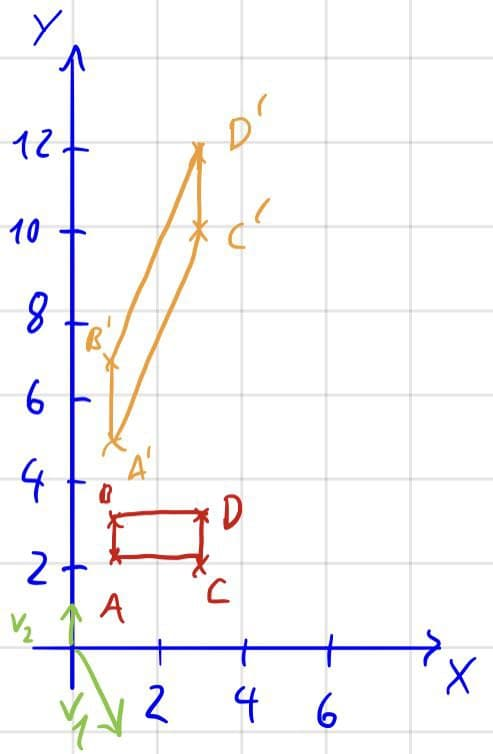
\includegraphics[width=.15\textwidth]{Dateien/02/02Anschauung1.jpg}
 \vspace{-15pt}
\end{wrapfigure}
Gegeben sei $F:\mathbb{R}^2\to\mathbb{R}^2,\,\Vec{v}\mapsto A_F\Vec{v}$ mit der darstellenden Matrix\\
$A_F=\MatrixInline{1&0\\2&2}$.\\
Sei nun $R$ ein Rechteck mit den Eckpunkten\\
$A=\MatrixInline{1\\2},\,B=\MatrixInline{1\\3},\,C=\MatrixInline{3\\2},\,D=\MatrixInline{3\\3}$.\\
Das Bild des Rechtecks können wir dann auch ermitteln.
Wir kennzeichnen die Eckpunkte des Bildes mit einem $'$:
\begin{equation*}
    A_F(A):=A'=\Matrix{1&0\\2&2}\Matrix{1\\2}=\Matrix{1\\6},\,B'=\Matrix{1\\8},\,C'=\Matrix{3\\10},\,D'=\Matrix{3\\12}.
\end{equation*}
Wir berechnen die Eigenwerte von $A$ mithilfe des charakteristischen Polynoms\\ $P_F(\lambda)=(1-\lambda)(2-\lambda)$ und lesen ab, dass $\lambda_1=1$ und $\lambda_2=2$.\\
Wir suchen die Eigenvektoren mithilfe der Eigenwertgleichung $A\Vec{v}=\lambda \Vec{v}\iff (A-\lambda\mathds{1}_2)\Vec{v}=\Vec{0}$ und verwenden dafür die Gaußschreibweise:
\begin{align*}
    \lambda_1:&\,\MatrixInvertieren{0&0\\2&1}{0\\0}\to x=t, \,y=-2t\implies \Vec{v}_1=t\Matrix{1\\-2}\to \tx{ER: } \Spann{\Matrix{1\\-2}}\\
    \lambda_2:&\, \MatrixInvertieren{-1&0\\2&0}{0\\0}\overset{\II+2\I}{\longrightarrow}\MatrixInvertieren{-1&0\\0&0}{0\\0}\to y=t,\,x=0\implies \Vec{v}_2=t\Matrix{0\\1}\to\tx{ER: }\Spann{\Matrix{0\\1}}.
\end{align*}
Wir sehen in der Skizze, dass jegliche Verbindungen in y-Richtung um den Faktor 2 gestreckt werden. Dies ist quasi genau der zweite Eigenwert/Eigenvektor.\\
Im Übrigen stellt die Matrix also eine Scherung im $\mathbb{R}^2$ dar, die, weil $\det A_F=2$, den Flächeninhalt geometrischer Figuren verdoppelt und dabei die Orientierung erhält.\\
Die Fixpunkte sind die Eigenvektoren, d. h. eine Figur mit Kanten, die diesen entsprechen, würde nicht geschert werden.\\
Betrachten wir folgendes Parallelogramm, das die Eigenvektoren von $A_F$ als Kanten hat:
\begin{align*}
    P_A&=\Matrix{0\\0},\,P_B=\Matrix{0\\2},\,P_C=\Matrix{1\\0},\,P_D=\Matrix{1\\-2}\\
    \to A(P_A):=P_A'&=\Matrix{1&0\\2&2}\Matrix{0\\0}=\Matrix{0\\0},\,P_B'=\Matrix{0\\4},\,P_C'=\Matrix{1\\2},\,P_D'=\Matrix{1\\-2}.
\end{align*}
\begin{center}
    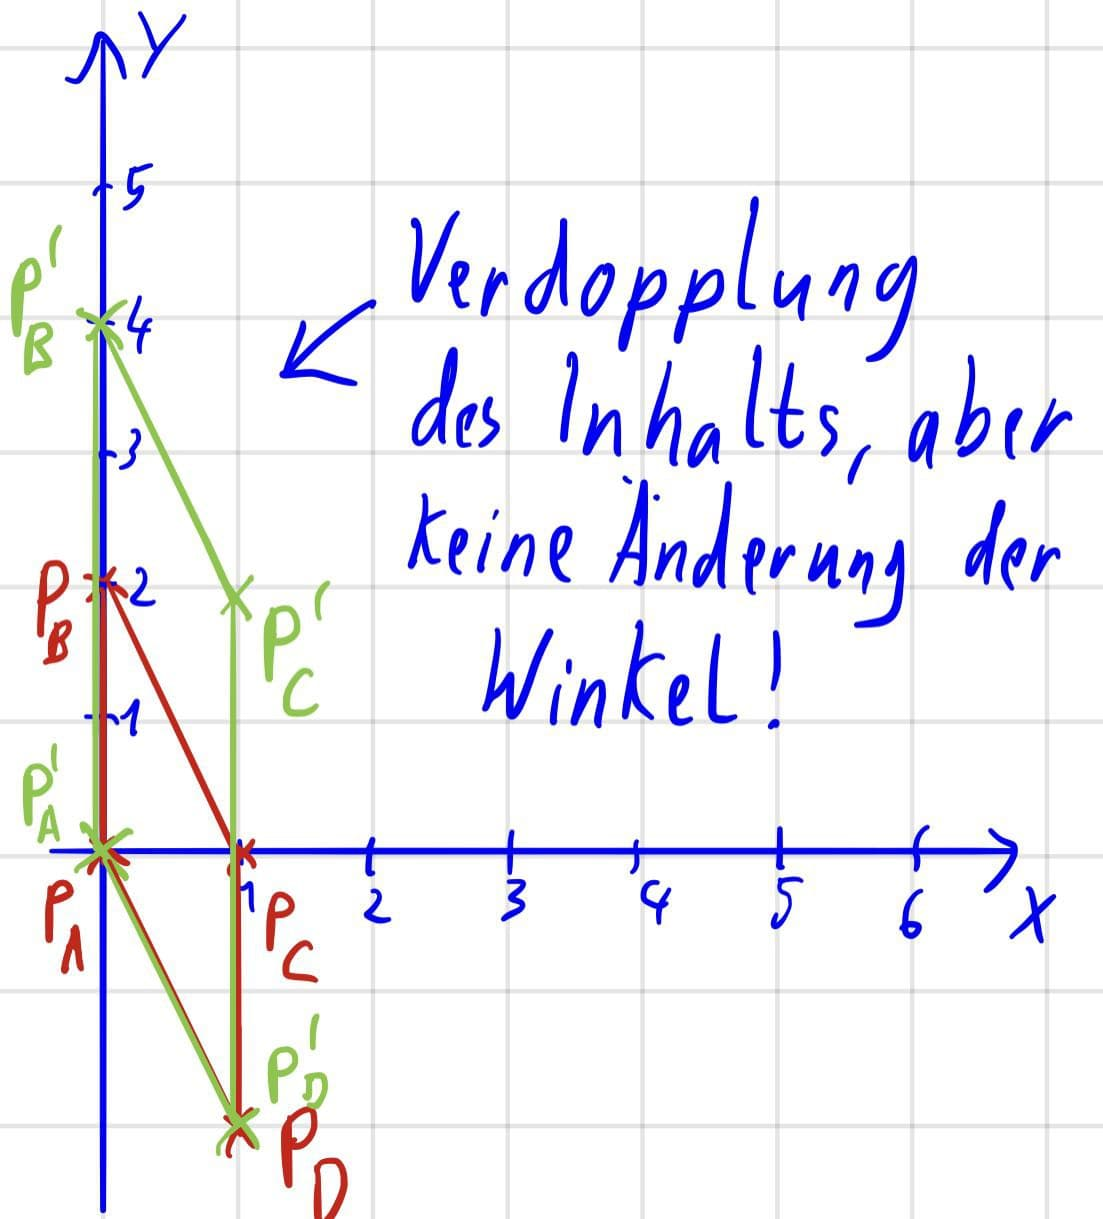
\includegraphics[width=.25\textwidth]{Dateien/02/02Anschauung2.jpg}
\end{center}
Es wird durch also tatsächlich nur geschert.
\end{Beispiel}


\Tipps{2}{
\begin{enumerate}
    % \item Orientiert euch an unseren Beispielen und überprüft genau, ob alle Axiome für eine Äquivalenzrelation erfüllt sind. Bei a) ist mit der Standard-Abstandsfunktion einfach $d(x,y)=\Abs{x-y}$ gemeint.\\
    % Beachtet bei b), dass nur alle durch drei teilbaren ganzen Zahlen gemeint sind (damit es nicht schon an der Reflexivität scheitert - sonst wäre nämlich z. B. $x=2$ nicht zu sich selbst äquivalent, da $2+2=4$ nicht durch 6 teilbar ist. Bei der Transitivität lohnt sich bei b) ein Blick auf den Beweis der Reflexivität.\footnote{Falls diese Aussage stimmen solte ;)}
    \item Das Invertieren der Matrix sollte mit unseren Beispielen von letzter Woche kein Problem sein. Mithilfe der Determinanten könnt ihr (zumindest notwendig) überprüfen, ob ihr richtig liegt.\footnote{Wenn ihr ganz sichergehen wollt, könnt ihr natürlich auch $A^{-1}A$ berechnen.}
    \item Hierzu b) gibt Robin in unserem Tutorium noch ein paar Tipps. 
    \item Dies ist ein Einzeiler. Startet mit der Definition des Betrages und macht euch dann klar, wie eine Matrix mit $(\overline{u_{ji}})$ aussieht.
    % \item \begin{enumerate}
    %     \item Hier hilft es, die Linearität der Determinante auszunutzen - welche Spalte bietet sich dafür an? Denkt dann an den Gauß-Algorithmus.\\
    %     Ihr solltet bei einem Ausdruck der Form
    %     \begin{equation*}
    %         \det A= \prod_{i=1}^n a_i+\sum_{k=1}^nb_k\prod_{j\neq k}^n c_j
    %     \end{equation*}
    %     kommen.
    %     \item Wir sehen leider nicht, wie man das mit Induktion macht, wir haben das mithilfe eines direkten Beweises und Aufgabe 3a) gemacht. Auch hier gilt wieder: Linearität ausnutzen!\\
    %     Weiterer Tipp (der in ähnlicher Form vielleicht nützlich ist):
    %     \begin{equation*}
    %         \det\Matrix{a_1&a_2&a_3\\a_1&a_2&a_3\\a_1&a_2&a_3}=\prod_{i=1}^3a_i\det\Matrix{1&1&1\\1&1&1\\1&1&1}
    %     \end{equation*}
    % \end{enumerate}
    \item Geht ganz klassisch nach dem Induktionsprinzip vor. Für den Induktionsanfang schaut euch noch einmal an, wie das leere Produkt definiert ist.\\
    Der Rest der Induktion ist ziemlich kompliziert, ihr könnt z. B. folgendermaßen vorgehen: Für $n+1$ wollt ihr ja irgendwie darauf hinaus, die Induktionsvoraussetzung einzusetzen. Dafür müsst ihr unter anderem die Linearität (bzw. Gauß'sche Umformungen) ausnutzen, um eine entspannte Laplace-Entwicklung machen zu können.\\
    Die entwickelte Matrix müsst ihr vermutlich ein bisschen länger angucken, Stichwort \textit{Determinantenmultiplikationssatz}.\\
    Wir hoffen, dass das hilft, lasst euch nicht von dem kompliziert aussehenden Produkt entmutigen, ihr schafft das! :)
    \item Hier ganz stumpf wie vorgeschlagen den Laplaceschen Entwicklungssatz auf $P_A(\lambda)=\det(A-\lambda\mathds{1}_n)$ anwenden.\\
    Heraus kommen sollte eine Summe der Form $\sum_{k=0}^{n-1}a_k$ (bzw. $\sum_{k=1}^nb_k$ wenn ihr den Index anders wählt).\\
    Anschließend müsst ihr mit vollst. Induktion zeigen, dass dies richtig ist. Auch hier hilft Laplace!
\end{enumerate}
}
\section[Diagonalisierung und Skalarprodukt]{Diagonalisierung, Bilinearformen, Skalarprodukt und Orthonormalbasen}
\Einleitung{Diese Woche ernten wir die Früchte unserer wochenlangen Vorarbeit: Wir sehen, dass die darstellende Matrix einiger Endomorphismen\footnote{Ein allerletztes Mal: Lineare Abbildungen eines Vektorraums in sich selbst.} bezüglich bestimmter Basen von $V$ eine Diagonalgestalt annimmt.\\
Diese bestimmten Basen setzen sich aus den Eigenvektoren des Endomorphismus zusammen. Wir betrachten also, unter welchen Bedingungen das möglich ist, und wechseln dann zum nächsten Thema:\\
Linearformen schnappen sich einzelne Vektoren und bilden sie auf Zahlen ab,\footnote{in diesem Zusammenhang hattet ihr den Dualraum kennengelernt}  während Bilinearformen sich jeweils zwei Vektoren schnappen und diese je auf eine Zahl abbilden. Diese Abbildungen müssen dabei u.a. linear sein. Unter bestimmten Umständen nennen wir eine Bilinearform auch (euklidisches\footnote{solange wir uns auf die reellen Zahlen $\mathbb{R}$ beziehen. Wir werden auch noch hermitesche Skalarprodukte kennenlernen, die für komplexe Vektorräume relevant sind.}) Skalarprodukt. Einen reellen Vektorraum mit einer solchen Abbildung bezeichnen wir dann als euklidisch, und wir sehen, dass sie sogar ausgezeichnete Basen (die Orthonormalbasen) haben.}

\subsection{Diagonalisierung von Endomorphismen}
\begin{Def}{Diagonalisierbarkeit}
Wir nennen einen Endomorphismus $F\in\End(V)$ \red{diagonalisierbar}, wenn eine Basis $B=(\bvec_1,...,\bvec_n)$ von $V$ existiert, bezüglich derer die darstellende Matrix $M_B(F)$ von $F$ \red{Diagonalgestalt} hat, d. h.
\begin{equation}
    M_B(F)=\diag(\lambda_1,\ldots,\lambda_n)=:\Matrix{\lambda_1&\cdots&\cdots&0\\
    \vdots&\lambda_2&&\vdots\\
    \vdots& & \ddots &\vdots\\
    0&\cdots&\cdots&\lambda_n},\quad\lambda_i\in\mathbb{K}\,\forall i
\end{equation}
\blue{Diese besondere Basis besteht aus den Eigenvektoren $\bvec_i$ von $F$ und die Diagonalelemente sind genau die Eigenwerte $\lambda_i$ dazu.}
\end{Def}
\blue{Um einen Endomorphismus zu diagonalisieren, müssen wir also die Eigenvektoren finden, und es muss genau $n=\dim V$ linear unabhängige Eigenvektoren geben, damit er diagonalisierbar ist. Letzteres ist auch die Aussage der folgenden Sätze:}
\begin{Satz}
{Satz}{Zerfall in Linearfaktoren}
Ist $F$ diagonalisierbar, so zerfällt das charakteristische Polynom $P_F(\lambda)$ in Linearfaktoren.
\end{Satz}
\blue{Das bedeutet, dass $P_F(\lambda)$ in der Form
\begin{equation*}
    P_F(\lambda)=\alpha\prod_{i=1}^n(\lambda-\lambda_i),\quad \alpha\in\mathbb{R}
\end{equation*}
geschrieben werden kann.\\
Da das charakteristische Polynom nicht von der Wahl der Basis abhängt, können wir es auch einfach mit der diagonalisierten Matrix berechnen:
\begin{equation*}
    P_F(\lambda)=\det(M_B(F)-\lambda\mathds{1}_n)=\prod_{i=1}^n(\lambda_i-\lambda).
\end{equation*}
Die Umkehrung gilt aber nur in bestimmten Fällen. Daher kann es auch wichtig sein, über welchem Körper euer Vektorraum definiert ist:\\
So zerfällt z. B. $P_F(\lambda)=(\lambda^2+1)=(\lambda+i)(\lambda-i)$ nur über $\mathbb{C}$ in Linearfaktoren, über $\mathbb{R}$ ist eine solche Zerlegung nicht möglich.}\\
Allerdings wissen wir noch nicht sicher, ob ein Endomorphismus diagonalisierbar ist, nur weil dessen charakteristisches Polynom in Linearfaktoren zerfällt. Entscheidend ist zudem die Dimension der zugehörigen Eigenräume, was in folgendem Satz festgehalten wird:
\begin{Satz}
{Satz}{Zur Diagonalisierbarkeit}
Für $F\in\End(V)$ (wobei $V$ endlichdimensional sei) gilt die folgende Äquivalenz:
\begin{itemize}
    \item $F$ ist diagonalisierbar.
    \item $P_F(\lambda)$ zerfällt in Linearfaktoren \underline{und} die geometrische und algebraische Vielfachheit stimmt für alle Eigenwerte überein, $n_{\lambda_i}=m_{\lambda_i}\,\forall \lambda_i$.
    \item $V$ ist die direkte Summe aus den Eigenräumen:\footnote{Dies ist eigentlich nur ein abstrakter Weg um zu sagen, dass die Vereinigung der Basisvektoren der Eigenräume eine Basis von $V$ bilden.} $V=\underset{\lambda\in\tx{EW}}{\bigoplus}V_\lambda$.
\end{itemize}
\end{Satz}
\blue{Jetzt seht ihr hoffentlich, weshalb wir uns letzte Woche die algebraische\footnote{Exponent des Eigenwertes im charakteristischen Polynom} und geometrische\footnote{Dimension des Eigenraums zum Eigenwert} Vielfachheit so genau angesehen haben.}
\begin{Satz}
{Kochrezept}{Diagonalisierung von Endomorphismen}
Um Endomorphismen zu diagonalisieren (oder zu testen, ob das überhaupt möglich ist), kann man auch nach folgendem Schema vorgehen:\\
Sei $(F:V\to V)\in\End(V)$ mit $\dim V=n$.
\begin{enumerate}
    \item (Ermittle die darstellende Matrix $A$ von $F$ bzgl. irgendeiner Basis\footnote{i. d. R. der kanonischen Basis}. Ist oft auch direkt gegeben.)
    \item Stelle das charakteristische Polynom auf: $P_A(\lambda)=\det(A-\lambda\mathds{1}_n)$.
    \item Ermittle die Nullstellen des charakteristischen Polynoms: $P_A(\lambda)=0$.\\
    Die ermittelten $\lambda_i$ sind die Eigenwerte.\\
    Zerfällt das charakteristische Polynom \textit{nicht} in Linearfaktoren, d. h. $\sum_{\lambda_i}m_{\lambda_i}<\dim V$, so ist $F$ nicht diagonalisierbar.
    \item Bestimme zu jedem $\lambda_i$ die Eigenvektoren $\bvec_{\lambda_i,j}$,\footnote{Dies können für einen Eigenwert $\lambda_i$ auch mehrere linear unabhängige sein, aber immer $\leq$ algebraische Vielfachheit des Eigenwerts.} indem $(A-\lambda_i\mathds{1}_n)\bvec_{\lambda_i,j}=\Vec{0}$ gelöst wird.
    \item Schreibe daraus die jeweiligen Eigenräume (als Span aus linear unabhängigen Eigenvektoren) auf.
    \item Ist die Summe der Dimensionen der Eigenräume $n$?
    \begin{enumerate}
        \item Wenn nein, so ist $F$ nicht diagonalisierbar.
        \item Wenn ja, so ist $F$ diagonalisierbar mit der darstellenden Matrix
        \begin{equation*}
            M_B(F)=\diag(\lambda_1,\ldots,\lambda_m)=\Matrix{\lambda_1&\cdots&\cdots&0\\
    \vdots&\lambda_2&&\vdots\\
    \vdots& & \ddots &\vdots\\
    0&\cdots&\cdots&\lambda_m}.
        \end{equation*}
        Hierbei tritt ein Eigenwert genau so oft auf, wie die Dimension des Eigenraumes ist.\footnote{Wenn zu $\lambda_i$ z. B. $n_{\lambda_i}=2$ ist, so tritt $\lambda_i$ zweimal auf der Diagonalen auf.}\\
        Die Eigenvektoren $\bvec_{\lambda_i,j}$ bilden dann genau die Basis $B=(\bvec_1,...,\bvec_n)$, bezüglich derer $F$ die Diagonalgestalt annimmt.
    \end{enumerate}
\end{enumerate}
\end{Satz}
Dieses Kochrezept wollen wir uns an folgendem Beispiel klar machen:
\begin{Beispiel}{Anwendung des Kochrezepts}
Sei $F:\mathbb{K}^3\to \mathbb{K}^2,\quad F(x,y,z)=\Matrix{x+3z\\y\\2x+z}$.\\
Ist $F$ über $\mathbb{R}$ bzw. über $\mathbb{C}$ diagonalisierbar?
\begin{enumerate}
    \item Bezüglich der kanonischen Basis $\hat{B}$ lesen wir ab:\footnote{Schaut euch einfach an, was $F$ mit den Einheitsvektoren macht, um die Einträge der Matrix zu bestimmen. Die erste Spalte ist das, was $F$ mit $\evec_1=\MatrixInline{1\\0\\0}$ macht usw.}
    \begin{equation*}
        A:=M_{\hat{B}}(F)=\Matrix{1&0&3\\0&1&0\\2&0&1}.
    \end{equation*}
    Wir sehen, dass $A\MatrixInline{x\\y\\z}=F(x,y,z)$ ist.
    \item Das charakteristische Polynom ist
    \begin{eqnarray*}
        P_A(\lambda)&=&\det\Matrix{1-\lambda&0&3\\0&1-\lambda&0\\2&0&1-\lambda}\\
        &\overset{\footnote{Regel von Sarrus}}{=}&(1-\lambda)^3-6+6\lambda\overset{\footnote{Binomischer Lehrsatz}}{=}1+3\lambda^2-3\lambda-\lambda^3-6+6\lambda\\
        &=&-\lambda^3+3\lambda^2+3\lambda-5.
    \end{eqnarray*}
    \item Wir raten die erste Nullstelle: $\lambda_1=1$. Mit Polynomdivision finden wir:
    \begin{equation*}
        P_F(\lambda):(\lambda-1)=-\lambda^2+2\lambda+5
    \end{equation*}
    Setzen wir dies gleich 0 und wenden nach Multiplikation mit $(-1)$ die $p$-$q$-Formel an, so finden wir
    \begin{equation*}
        \lambda_{2,3}=1\pm \sqrt{6},
    \end{equation*}
    es gilt also
    \begin{equation*}
        P_A(\lambda)=(\lambda-1)(\lambda-1+\sqrt{6})(\lambda-1-\sqrt{6}).
    \end{equation*}
    Das charakteristische Polynom zerfällt also in Linearfaktoren mit den jeweiligen algebraischen Vielfachheiten von 1.
    \item Wir suchen die Eigenvektoren zu den verschiedenen Eigenwerten, indem wir die Eigenwertgleichung $A\Vec{v}=\lambda \Vec{v}$ lösen:
    \begin{itemize}
        \item Zu $\lambda_1=1$:
        \begin{align*}
            &\MatrixInvertieren{1-1&0&3\\0&1-1&0\\2&0&1-1}{0\\0\\0}=\MatrixInvertieren{0&0&3\\0&0&0\\2&0&0}{0\\0\\0}\\
            &\implies 0x_2=0\implies x_2=t_1\in\mathbb{K},\,x_1=0=x_3.
        \end{align*}
        Also sehen wir: $\bvec_1=t_1\MatrixInline{0\\1\\0}$.
        \item Zu $\lambda_2=1-\sqrt{6}$:
        \begin{equation*}
            \MatrixInvertieren{\sqrt{6}&0&3\\0&\sqrt{6}&0\\2&0&\sqrt{6}}{0\\0\\0}\implies x_2=0,\, x_1=-\frac{\sqrt{6}}{2}x_3\implies x_3=t_2\in\mathbb{K}.
        \end{equation*}
        Also sehen wir: $\bvec_2=t_2\MatrixInline{-\sqrt{6}/2\\0\\1}$.
        \item Zu $\lambda_3=1+\sqrt{6}$:
        \begin{equation*}
            \MatrixInvertieren{-\sqrt{6}&0&3\\0&-\sqrt{6}&0\\2&0&-\sqrt{6}}{0\\0\\0}\implies x_2=0,\, x_1=\frac{\sqrt{6}}{2}x_3\implies x_3=t_3\in\mathbb{K}.
        \end{equation*}
        Also sehen wir: $\bvec_3=t_3\MatrixInline{\sqrt{6}/2\\0\\1}$.
        \item Die Eigenräume sind dann also
        \begin{align*}
            \lambda_1&=1:\quad V_1=\Spann{\MatrixInline{0\\1\\0}}\\
            \lambda_2&=1-\sqrt{6}:\quad V_1=\Spann{\MatrixInline{-\sqrt{6}/2\\0\\1}}\\
            \lambda_3&=1+\sqrt{6}:\quad V_1=\Spann{\MatrixInline{\sqrt{6}/2\\0\\1}}.
        \end{align*}
        Die geometrische Vielfachheit ist jeweils $n_{\lambda_i}=\dim V_{\lambda_i}=1=m_{\lambda_i}$.
        \item Für alle Eigenwerte ist $n_{\lambda_i}=m_{\lambda_i}$ und $\sum_{i=1}^3\dim V_{\lambda_i}=3=\dim(\mathbb{K}^3)$.\\
        Die diagonalisierte Matrix ist daher
        \begin{equation*}
            M_B(F)=\diag(1,1-\sqrt{6},1+\sqrt{6})=\Matrix{1&0&0\\0&1-\sqrt{6}&0\\0&0&1+\sqrt{6}}.
        \end{equation*}
        Die zugehörige Basis ist $B=\MengeDirekt{\MatrixInline{0\\1\\0},\MatrixInline{-\sqrt{6}\\0\\2},\MatrixInline{\sqrt{6}\\0\\2}}$.\\
        $F$ ist also über $\mathbb{R}$ und somit auch über $\mathbb{C}$ diagonalisierbar.
    \end{itemize}
\end{enumerate}
\blue{Anmerkung:\\
Tatsächlich gilt $M_B(F)=\varphi_B^{-1}M_{\hat{B}}(F)\varphi_B$:\footnote{Hierbei ist $\varphi_B$ die Basiswechselmatrix zwischen der kanonischen Basis und der Basis $B$, die wir bestimmen, indem wir einfach die Basisvektoren spaltenweise aufschreiben.}
\begin{center}
    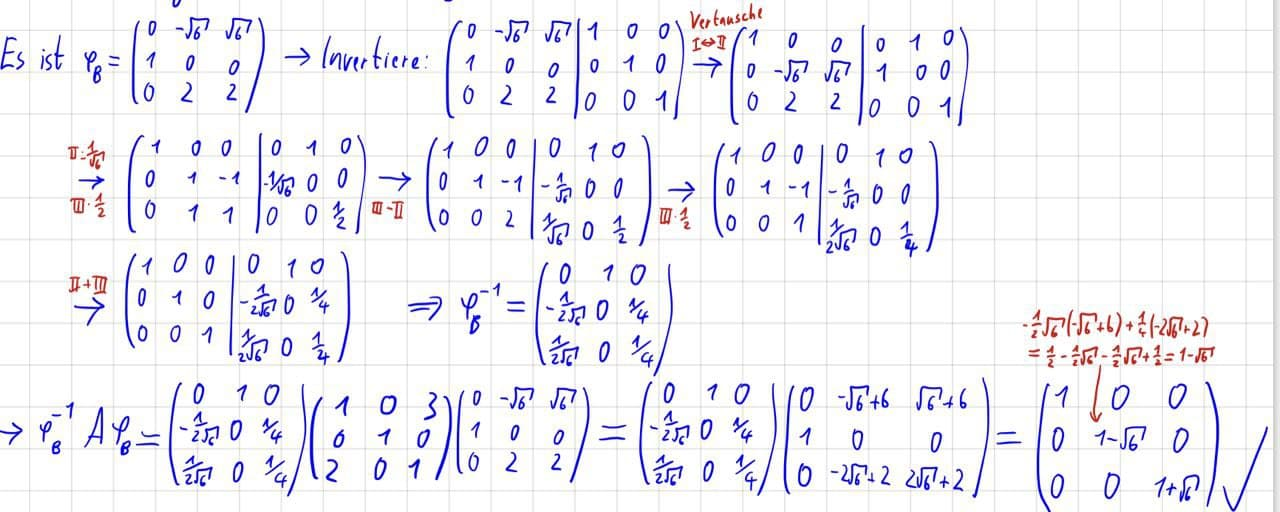
\includegraphics[width=.75\textwidth]{Dateien/03/03Diagonalisierung.jpg}
\end{center}}
\end{Beispiel}
\subsection{Längen- und Winkelmessungen mit Vektoren}
\blue{Unser nächstes Ziel ist nun, Längen, Abstände und Winkelbeziehungen zwischen Vektoren sinnvoll zu definieren. Wichtige Begriffe sind hierbei das Skalarprodukt, die Norm, Orthogonalität und die Cauchy-Schwarzsche Ungleichung.}


\subsubsection{Linearformen}
\begin{Wiederholung}
{Linearform}
Zunächst erinnern wir uns an den Begriff der \red{Linearform} aus MfP1:\\
Dies waren \underline{lineare Abbildungen}, die Elemente eines Vektorraumes $V$ über $\mathbb{K}$ in den Körper $\mathbb{K}$ abbilden, also $L\in L(V,\mathbb{K})$.\\
Die Menge aller solchen linearen Abbildungen wird \red{Dualraum} $V^*$ von $V$ genannt, also $V^*=\MengeDirekt{L:V\to\mathbb{K}}$.\\
Für endlichdimensionale Vektorräume $V$ mit $\dim V=n$ ist auch $\dim V^*=n$ und wir können die sog. \red{duale Basis} $B^*=(\bvec_1^*,\ldots,\bvec_n^*)$ zu einer Basis $B=(\bvec_1,\ldots,\bvec_n)$ von $V$ anhand folgender Forderung\footnote{die analog dazu ist, dass $\varphi_{B^*}\circ\varphi_B=\mathds{1}_n$ ist} definieren:
\begin{equation}
    \bvec_i^*(\bvec_j)=\delta_{ij}=\Cases{1&i=j\\0\,&i\neq j}.
\end{equation}
\blue{Zum Finden der dualen Basis kann man die Matrix aus Basisvektoren invertieren und dann die Zeilenvektoren als duale Basisvektoren ablesen.}\\
Die darstellende Matrix von Linearformen können wir uns als $1\times n$ Zeilenvektoren vorstellen.
\end{Wiederholung}
\begin{Beispiel}
{Linearform und darstellende Matrix über $\mathbb{R}$ (1/3)}
Wir betrachten den $\mathbb{R}^3$ mit der kanonischen Basis $\hat{B}=\MengeDirekt{\MatrixInline{1\\0\\0},\MatrixInline{0\\1\\0},\MatrixInline{0\\0\\1}}$. Die duale Basis wäre dann schlicht $\hat{B}^*=\MengeDirekt{\MatrixInline{1\\0\\0}^T,\MatrixInline{0\\1\\0}^T,\MatrixInline{0\\0\\1}^T}$, denn es gilt ja $\evec_i^*\evec_j=\delta_{ij}$.\\
Eine Linearform wäre z. B. die Abbildung $F:\mathbb{R}^3\to\mathbb{R},\, F(x,y,z)=2x-y+3z$. Diese hätte bzgl. $\hat{B}$ die folgende darstellende Matrix:
\begin{equation*}
    M_{\hat{B}}(F)=\Matrix{2&-1&3}\overset{\wedge}{=}2\evec_1^*-\evec_2^*+3\evec_3^*.
\end{equation*}
\end{Beispiel}
\begin{Beispiel}{Duale Basis im $\mathbb{C}^3$ (2/3)}
Sei  $B=\MengeDirekt{\MatrixInline{i\\0\\1},\MatrixInline{1\\1\\0},\MatrixInline{1\\1\\i}}$.\\
\Zz{Dies ist eine Basis von $\mathbb{C}^3$\footnote{Aufgefasst als Vektorraum über $\mathbb{C}$ - Als Vektorraum über $\mathbb{R}$ wären sechs Basisvektoren notwendig.} und die duale Basis ist\\ $B^*=\MengeDirekt{\MatrixInline{-i\\i\\0}^T,\MatrixInline{-1\\2\\i}^T,\MatrixInline{1\\-1\\-i}^T}$}
\Zb{$B$ ist eine Basis von $\mathbb{C}^3$, denn sie verfügt über drei linear unabhängige Vektoren, weil
\begin{equation*}
    \det \varphi_B=\det\Matrix{i&1&1\\0&1&1\\1&0&i}=i^2+1-1=-1\neq0.
\end{equation*}
Wir wollen nun die duale Basis finden. Wir suchen also $\varphi_{B^*}$, sodass $\varphi_{B^*}\circ \varphi_B=\mathds{1}_3$ ist. Es ist also nur die Inversion der Basismatrix $\varphi_B$ gefragt, und wir wissen ja, wie wir das machen:
\begin{align*}
    \MatrixInvertieren{i&1&1\\0&1&1\\1&0&i}{1&0&0\\0&1&0\\0&0&1}\overset{\I-\II,i\cdot\III}&{\longrightarrow}\MatrixInvertieren{i&0&0\\0&1&1\\i&0&-1}{1&-1&0\\0&1&0\\0&0&i}\\
    \overset{\III-\I,-i\cdot\I}&{\longrightarrow}\MatrixInvertieren{1&0&0\\0&1&1\\0&0&-1}{-i&i&0\\0&1&0\\-1&1&i}\\
    \overset{\II+\III,-1\cdot\III}&{\longrightarrow}\MatrixInvertieren{1&0&0\\0&1&0\\0&0&1}{-i&i&0\\-1&2&i\\1&-1&-i}.
\end{align*}
Wir lesen also ab: $\bvec_1^*=\Matrix{-i&i&0},\,\bvec_2^*=\Matrix{-1&2&i},\,\bvec_3^*=\Matrix{1&-1&-i}$.\\
Hierbei sind die $\bvec_i^*\in\Met(1,3,\mathbb{C})$ als lineare Abbildungen von $\mathbb{C}^3\to\mathbb{C}$ zu sehen.}\\
Wir betrachten nun die Abbildung $G:\mathbb{C}^3\to\mathbb{C},\, G(x,y,z)=x+y-iz$.\\
Wie sieht die darstellende Matrix dieser Abbildung bzgl. der Basis $B$ aus?\\
Wir nutzen die Gleichung $F(\vvec_j)=\sum_{i=1}^ma_{ij}\wvec_i,\,j=1,\ldots,n$ aus MfP1, um die darstellende Matrix zu bestimmen, wobei $v_j\in B$ und $\wvec_i\in B^*$ sind. Mit $V=\MengeDirekt{(1)}=:\MengeDirekt{\vvec_1}$ als Basis von $\mathbb{C}$ haben wir dann
\begin{align*}
    G(\bvec_1)&=i-i=0\overset{!}{=}a_{11}\vvec_1\\
    G(\bvec_2)&=1+1=2\overset{!}{=}a_{12}\vvec_1\\
    G(\bvec_3)&=1+1-i^2=3\overset{!}{=}a_{13}\vvec_1.
\end{align*}
Wir sehen also: $M_B^V(G)=\Matrix{0&2&3}$.\\
Diese Einträge könnten wir nun auch bzgl. der dualen Basis $B^*$ ausdrücken, aber das sparen wir uns.
\end{Beispiel}
\begin{Beispiel}
{Das Integral als Linearform (3/3)}
Für integrierbare Funktionen $R$\footnote{Mit $I$ bezeichnen wir für dieses Beispiel also den Raum der integrierbaren Funktionen auf $[a,b]$} ist das Integral $\int: I\to \mathbb{R},\,f(x)\mapsto\int_a^bf(x)dx$ eine Linearform.
\end{Beispiel}


\subsubsection{Multilinearformen und Eigenschaften von Bilinearformen}
Wir verallgemeinern nun das Konzept auf mehrere Elemente aus $V$, die linear auf ein Element des Körpers $\mathbb{K}$ abgebildet werden:
\begin{Def}
{Multilinearform}
Abbildungen $\mu: V^k\to\mathbb{K},\,(\vvec_1,\vvec_2,\ldots,\vvec_k)\mapsto\mu(\vvec_1,\ldots,\vvec_k)$ nennen wir \red{$k$-Linearform}, wenn $\mu$ in allen Argumenten linear\footnote{d. h. die beiden Bedingungen für Linearität, $F(\lambda \vvec+\wvec)=\lambda F(\vvec)+F(\wvec)$ in allen Argumenten erfüllt} ist.
\end{Def}
$k$-Linearformen mit $k>2$ werden uns für's Erste nicht mehr über den Weg laufen. Stattdessen nimmt die 2-Linearform eine wichtige Rolle ein:
\begin{Def}
{Bilinearform}
Für einen $\mathbb{K}$-Vektorraum $V$ nennen wir eine Abbildung\\
$\beta: V\times V\to \mathbb{K},\, (\vvec,\wvec)\mapsto\beta(\vvec,\wvec)$ \red{Bilinearform}, wenn sie linear in beiden Argumenten ist:\\
$\forall \vvec,\wvec,\zvec\in V$ und $\forall \lambda, \mu\in\mathbb{K}$ gilt dann
\begin{align*}
    &\beta(\lambda \vvec+\mu \wvec,\zvec)=\lambda\beta(\vvec,\zvec)+\mu \beta(\wvec,\zvec)\\
    &\beta(\vvec, \lambda \wvec+\mu \zvec)=\lambda\beta(\vvec,\wvec)+\mu\beta(\vvec,\zvec).
\end{align*}
\end{Def}
Bevor wir zu den Beispielen kommen, folgen noch ein paar wichtige Definitionen, um Bilinearformen zu klassifizieren:
\begin{Def}
{Symmetrie{,} Schiefsymmetrie und Entartung}
Wir nennen eine Bilinearform $\beta:V\times V\to \mathbb{K}$...
\begin{itemize}
    \item ...\red{symmetrisch} $\iff\beta(\vvec,\wvec)=\beta(\wvec,\vvec)\quad\forall \vvec,\wvec\in V$.
    \item ...\red{schiefsymmetrisch} $\iff\beta(\vvec,\wvec)=-\beta(\wvec,\vvec)\quad\forall \vvec,\wvec\in V$.
    \item ...\red{nicht entartet} $\iff$ Die Abbildung $V\to V^*,\,\vvec\mapsto \beta(\vvec,\cdot)$ ist injektiv\\
    $\quad\iff\beta(\vvec,\wvec)=0\quad\forall \wvec\in V$ nur wenn $\vvec=0$.
\end{itemize}
\blue{Mit der darstellenden Matrix werden wir gleich ein Werkzeug kennenlernen, mit dem man diese Eigenschaften schnell überblicken kann.}
\end{Def}
\blue{Tipp:\\
Wenn ihr zeigen wollt, dass eine symmetrische Abbildung eine Bilinearform ist, zeigt zuerst die Symmetrie.\\
Anschließend könnt ihr die Linearität im 1. Argument zeigen und für das 2. Argument einfach mit der Symmetrie argumentieren.}

\begin{Beispiel}
{Bilinearform auf dem $\mathbb{R}^3$}\label{03:beispBiFo}
Die Abbildung $\gamma:\mathbb{R}^3\times \mathbb{R}^3\to \mathbb{R}$ mit
\begin{equation*}
    \gamma(\vvec,\wvec)=3v_1w_1-v_2w_2+v_3w_3+2v_3w_1+2v_1w_3
\end{equation*}
ist eine symmetrische Bilinearform, denn\footnote{mit $\vvec=\MatrixInline{v_1\\v_2\\v_3}$ und $\wvec=\MatrixInline{w_1\\w_2\\w_3}$} $\gamma(\vvec,\wvec)=\gamma(\wvec,\vvec)$, sie ist also symmetrisch.\\
Wir zeigen nun die Linearität im 1. Argument: Für alle $\vvec,\wvec,\zvec\in\mathbb{R}^3,\,\lambda,\mu\in\mathbb{R}$ ist
\begin{align*}
    \gamma(\lambda v+\mu \wvec,\zvec)&=3(\lambda v_1+\mu w_1)z_1-(\lambda v_2+\mu w_2)z_2+(\lambda v_3+\mu w_3)z_3\\
    &\quad +2(\lambda v_3+\mu w_3)z_1+2(\lambda v_1+\mu w_1)z_3\\
    &=\lambda(3v_1z_1-v_2z_2+v_3z_3+2v_3z_1+2v_1z_3)\\
    &\quad+\mu(3w_1z_1-w_2z_2+w_3z_3+2w_3z_1+2w_1z_3)\\
    &=\lambda\gamma(\vvec,\zvec)+\mu\gamma(\wvec,\zvec).
\end{align*}
Aufgrund der Symmetrie ist $\gamma$ auch im 2. Argument linear.\\
Wir haben also gezeigt, dass $\gamma$ eine symmetrische Bilinearform ist.
\end{Beispiel}
\begin{Satz}
{Satz}{Bilinearformen haben eine darstellende Matrix}
Für $n$-dimensionale Vektorräume mit Basis $B=(\bvec_1,\ldots,\bvec_n)$ können wir der Bilinearform $\beta:V\times V\to \mathbb{K}$ eine \red{darstellende Matrix} bzgl. $B$ zuordnen, die eine $n\times n$-Matrix mit den Einträgen \underline{$\alpha_{ij}=\beta(\bvec_i,\bvec_j)$} ist.\\
\blue{Zum Finden der darstellenden Matrix müssen wir also nur gucken, was $\beta$ mit den Basisvektoren macht.}
\end{Satz}
\begin{Satz}{Satz}
{Aussagen über Bilinearformen}
Die darstellende Matrix $M_B(\beta)$ liefert uns einen schnellen Blick auf die Eigenschaften der Bilinearform:
\begin{itemize}
    \item Symmetrie $\iff M_B(\beta)=M_B(\beta)^T$, also z. B. $\MatrixInline{1&-2\\-2&-3}=\MatrixInline{1&-2\\-2&-3}^T$.
    \item Schiefsymmetrie $\iff M_B(\beta)=-M_B(\beta)^T$.
    \item Nicht-Entartung $\iff M_B(\beta)$ ist invertierbar $\iff\det M_B(\beta)\neq 0$.
\end{itemize}
\end{Satz}

\begin{Beispiel}
{Darstellende Matrix einer Bilinearform: Kanonische Basis (1/2)}
Wir wollen die darstellende Matrix der in \hyperref[03:beispBiFo]{Beispiel 3.5} definierten Bilinearform $\gamma$ mit
\begin{equation*}
    \gamma(\vvec,\wvec)=3v_1w_1-v_2w_2+v_3w_3+2v_3w_1+2v_1w_3
\end{equation*}
bzgl. der kanonischen Basis bestimmen:\\
Hierfür kann man mehr oder weniger ablesen: $\gamma(\evec_1,\evec_1)=3\cdot 1\cdot 1+0=3$ usw. Also ist
\begin{equation}
    A:=M_{\hat{B}}(\gamma)=\Matrix{3&0&2\\0&-1&0\\2&0&1}\implies A=A^T,
\end{equation}
$A$ ist also symmetrisch.\\
Ist $\gamma$ entartet?\\
Nein, denn $\det A\overset{\footnote{Sarrus}}{=}3(-1)1-2(-1)2=-3+4=1\neq0$.
\end{Beispiel}

\begin{Beispiel}
{Darstellende Matrix einer Bilinearform: Sonstige Basis (2/2)}
Nun wollen wir für $\gamma$ für die Basis $B=\MengeDirekt{\MatrixInline{1\\1\\0},\MatrixInline{0\\2\\2},\MatrixInline{-1\\0\\-1}}$ die darstellende Matrix bestimmen.\\
Hierfür müssen wir die einzelnen Einträge $\alpha_{ij}$ berechnen, indem wir die jeweiligen Basisvektoren $\bvec_i$ und $\bvec_j$ in $\gamma$ einsetzen:
\begin{align*}
    \alpha_{11}&=\gamma(\bvec_1,\bvec_1)=3\cdot 1\cdot -1\cdot 1+0\cdot 0+0=2\quad \alpha_{12}=0-2+0+0+4=4,\\
    \alpha_{13}&=-3+0+0+0-2=-5,\quad \alpha_{22}=-4+4+0=0,\quad \alpha_{23}=-2-4=-6,\\
    \alpha_{33}&=3-0+1+2+2=8,\quad \alpha_{21}=\alpha_{12}=4,\quad \alpha_{31}=\alpha_{13}=-5,\quad\alpha_{32}=-3
\end{align*}
Hierbei haben wir für die letzten Einträge die bekannte Symmetrie ausgenutzt. Wir sehen also:
\begin{equation*}
    A_2:=M_B(\gamma)=\Matrix{2&2&-5\\2&0&-6\\-5&-6&8}.
\end{equation*}
Ihr fragt euch vielleicht, wieso man sich den ganzen Aufwand macht und was man damit überhaupt \textit{darstellen} kann.\\
Mit der darstellenden Matrix können wir für $\gamma$ sehr schnell auswerten, was mit Vektoren bzgl. der Basis geschieht.\\
Als Beispiel betrachten wir $\vvec_1:=2\bvec_1+\bvec_3$ und $\vvec_2:=\bvec_2-\bvec_3$.\\
Verschiedene Wege führen nun zu $\gamma(\vvec_1,\vvec_2)$:
\begin{itemize}
    \item Zunächst können wir $\vvec_1$ und $\vvec_2$ bzgl. der kanonischen Basis darstellen:
    \begin{equation*}
        \vvec_1=2\Matrix{1\\1\\0}+3\Matrix{-1\\0\\-1}=-\evec_1+2\evec_2-3\evec_3,\quad \vvec_2=\Matrix{0\\2\\2}-\Matrix{-1\\0\\-1}=\evec_1+2\evec_2+3\evec_3.
    \end{equation*}
    Damit ist dann
    \begin{align*}
        \gamma(\vvec_1,\vvec_2)&=\Matrix{-1&2&-3}\Matrix{3&0&2\\0&-1&0\\2&0&1}\Matrix{1\\2\\3}=\Matrix{-1&2&-3}\Matrix{9\\-2\\5}\\
        &=-9-4-15=-28.
    \end{align*}
    Achtung: Im ersten Schritt haben wir $\vvec_1$ bzgl. der dualen Basis dargestellt, was im Falle der kanonischen Basis einfach das Transponieren bedeutet. Im Allgemeinen müsst ihr hier aber vorsichtig sein.
    \item Explizite Berechnung:
    \begin{equation*}
        \gamma(\vvec_1,\vvec_2)=3(-1)-2\cdot 2+(-3)3+2(-3)1+2(-1)3=-3-4-9-6-6=-28
    \end{equation*}
    \item Indem wir $\vvec_1$ bzgl. der dualen Basis darstellen, würden wir finden, dass
    \begin{equation*}
        \gamma(\vvec_1,\vvec_2)=\vvec_1^*\cdot A\cdot \vvec_2=-28
    \end{equation*}
    ist. Allerdings sparen wir uns an dieser Stelle das Finden der dualen Basis und das Darstellen von $\vvec_1$, ihr könnt es gern als Übung machen, als Überprüfung seht ihr ja das Ergebnis.
\end{itemize}
\end{Beispiel}

\subsubsection{Das Skalarprodukt als Spezialfall von Bilinearformen}
\begin{Def}
{Positive Definitheit}
Eine weitere Eigenschaft, die wir \underline{symmetrischen} Bilinearformen zuschreiben, ist die \red{positive Definitheit}, wir nennen $\beta:V\times V\to \mathbb{K}$ positiv definit, wenn
\begin{equation}
    \beta(\vvec,\vvec)>0 \quad \forall v\in V\tx{ mit } v\neq0.
\end{equation}
Wir schreiben ab jetzt $\beta(\vvec,\wvec)=:\BiFo{\vvec,\wvec}$ und meinen damit symmetrische Bilinearformen $\BiFo{\cdot,\cdot}:V\times V\to \mathbb{K}$.
\end{Def}

\begin{Def}
{(Euklidisches) Skalarprodukt}
Ein \red{euklidisches Skalarprodukt} auf $V$ ist eine \underline{positiv definite} \underline{symmetrische Bilinearform} $V\times V\to \mathbb{R}$ auf einem reellen Vektorraum $V$.
\end{Def}
\begin{Def}
{Euklidischer Vektorraum}
Ist auf einem \underline{reellen} Vektorraum ein Skalarprodukt definiert, nennen wir ihn \red{euklidisch}.
\end{Def}
\begin{Satz}
{Kochrezept}{Skalarprodukt zeigen}
Um zu zeigen, dass eine Abbildung $V\times V\to\mathbb{R}$ ein eukl. Skalarprodukt ist, müssen wir also zeigen:
\begin{enumerate}
    \item Positive Definitheit:\\
    $\BiFo{\vvec,\vvec}=0\implies \vvec=0\quad \vvec\in V$\\
    $v=0\implies \BiFo{\vvec,\vvec}=0$\\
    $\BiFo{\vvec,\vvec}>0\quad \forall \vvec\neq 0$.
    \item Symmetrie:\\
    $\BiFo{\vvec,\wvec}=\BiFo{\wvec,\vvec}\quad \forall \vvec,\wvec\in V$.
    \item Bilinearität:\\
    $\BiFo{\lambda \uvec+\vvec,\wvec}=\lambda\BiFo{\uvec,\wvec}+\BiFo{\vvec,\wvec}$.\\
    Die Linearität im zweiten Argument folgt dann aus der Symmetrie.
\end{enumerate}
\end{Satz}
\begin{Beispiel}
{Das kanonische Skalarprodukt}
Das kanonische Skalarprodukt im $\mathbb{R}^n$ ist definiert als\\
$\BiFo{\cdot,\cdot}:\mathbb{R}^n\times\mathbb{R}^n\to\mathbb{R},\quad \BiFo{\Vec{x},\Vec{y}}=\sum_{i=1}^nx_iy_i$.\\
Dieses sollten die meisten von euch bereits aus der Schule oder Physikvorlesungen kennen. Am besten überlegt ihr kurz, ob und warum hier alle geforderten Eigenschaften erfüllt sind.
\end{Beispiel}
Konzeptionell ist es für euch wahrscheinlich zunächst seltsam, dass nicht nur das euch bekannte kanonische Skalarprodukt existiert, sondern dass der Begriff eigentlich viel allgemeiner gefasst ist und das kanonische nur ein Spezialfall ist. Gewöhnt euch dran, das gleiche passiert nun mit den Definitionen von Längen von Vektoren (der Norm) und Abständen von Vektoren.

\subsubsection{Die Vermessung von Vektorräumen: Normen, Metriken, Winkel und Orthogonalität}
\begin{Def}
{Vom Skalarprodukt induzierte Norm}
In euklidischen Vektorräumen bezeichnen wir mit $\boxed{\Norm{\vvec}:=\sqrt{\BiFo{\vvec,\vvec}}}$ die \red{Länge} bzw. \red{Norm} eines Vektors.\\
\blue{Achtung:\\
Auch auf nicht euklidischen Vektorräumen\footnote{also jenen ohne Skalarprodukt} kann man eine Norm definieren!\footnote{Diese muss dann, ähnlich wie die Metrik oder das Skalarprodukt, bestimmte Eigenschaften erfüllen. Dazu später mehr.} Genau genommen ist diese Definition nur die \textit{vom Skalarprodukt induzierte} Norm.}
\end{Def}
Den folgenden Begriff hattet ihr im Zusammenhang mit der Betragsmetrik auf $\mathbb{R}$ bzw. $\mathbb{C}$ schon kennengelernt:
\begin{Wiederholung}
{Metrik}
Eine \red{Metrik} ist eine Abbildung auf einer Menge $X$ mit der Form $d:X\times X\rightarrow \mathbb{R}_+\cup \{0\}$ mit den Eigenschaften
\begin{eqnarray*}
\red{M1}: & d(x,y)\geq 0\text{ und } d(x,y)=0\Leftrightarrow x= y &\red{'positiv definit'}\\
\red{M2}: & d(x,y)=d(y, x) &\red{'symmetrisch'}\\
\red{M3}: & d(x,y)\leq d(x, z)+d(y,z) & \red{'Dreiecksungleichung'}.
\end{eqnarray*}
\end{Wiederholung}
\begin{Def}
{Durch das Skalarprodukt induzierte Metrik}
Mithilfe dieser Längendefinition können wir uns den \red{Abstand} zwischen zwei Punkten $\xvec,\yvec\in V$ definieren:
\begin{equation}
    \boxed{d(\xvec,\yvec)=\Norm{\xvec-\yvec}=\sqrt{\BiFo{\xvec-\yvec,\xvec-\yvec}}}.
\end{equation}
Da hier immer ein Skalarprodukt zugrunde liegt, nennt man diesen Abstandsbegriff auch die \red{vom Skalarprodukt induzierte Metrik}.\\
\blue{Achtung:\\
Ist auf einem Vektorraum nur eine Norm definiert, so reicht das auch aus und wir nennen $d(\xvec,\yvec)=\Norm{\xvec,\yvec}$ die \red{von der Norm induzierte Metrik}. Allerdings ist selbst eine Norm nicht notwendig, Metriken können auch einfach so definiert werden, solange sie die Metrikaxiome erfüllen.}
\end{Def}
\begin{Satz}
{Satz}{Cauchy-Schwarzsche Ungleichung}
Für alle $\vvec,\wvec$ in einem euklidischen Vektorraum gilt:
\begin{equation}
    \boxed{\Abs{\BiFo{\vvec,\wvec}}\leq\Norm{\vvec}\cdot\Norm{\wvec}},
\end{equation}
wobei Gleichheit genau bei linearer Abhängigkeit von $\vvec$ und $\wvec$ gilt.
\end{Satz}
\blue{Diese Ungleichung ist auch in der Physik super wichtig.}
\begin{Beispiel}
{Cauchy-Schwarz für das kanonische Skalarprodukt}
Bzgl. des kanonischen Skalarprodukts im $\mathbb{R}^n$ sieht das dann so aus:
\begin{equation*}
    \Abs{\BiFo{\xvec,\Vec{y}}}=\Abs{\sum_{i=1}^nx_iy_i}\leq\sqrt{\sum_{i=1}^nx_i^2}\sqrt{\sum_{j=1}^ny_j^2}=\sqrt{\BiFo{\xvec,\xvec}}\sqrt{\BiFo{\yvec,\yvec}}=\Norm{\xvec}\cdot \Norm{\yvec}.
\end{equation*}
\end{Beispiel}

\begin{Def}
{Winkel}
Für $\vvec,\wvec\in V\setminus\MengeDirekt{\Vec{0}}$ ist der Winkel zwischen $v$ und $w$ definiert als
\begin{equation}
    \angle(\vvec,\wvec):=\arccos\frac{\BiFo{\vvec,\wvec}}{\Norm{v}\cdot\Norm{w}}\in[0,\pi]
\end{equation}
\end{Def}
\begin{Def}
{Orthogonalität}
Bei einem Winkel von $\pi\overset{\wedge}{=}90^\circ$ nennen wir $\vvec$ und $\wvec$ \red{orthogonal}. In diesem Fall gilt
\begin{equation}
    \BiFo{\vvec,\wvec}=0
\end{equation}
\end{Def}
\begin{wrapfigure}{r}[0pt]{.15\textwidth}
 \vspace{-15pt}
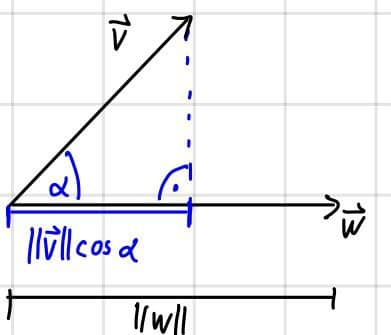
\includegraphics[width=.15\textwidth]{Dateien/03/03CauchySchwarz.jpg}
 \vspace{-5pt}
\end{wrapfigure}
\blue{Damit wird die Cauchy-Schwarzsche Ungleichung eventuell auch klarer:\\
Das Skalarprodukt projiziert den einen Vektor auf den anderen (daher der $\cos(\angle(\vvec,\wvec))$) und multipliziert die Beträge der Längen:\\
Die Projektion verschwindet genau bei Orthogonalität, bei linearer Abhängigkeit ist $\Abs{\BiFo{\vvec,\wvec}}=\Norm{\vvec}\cdot\Norm{\wvec}$.}


\subsubsection{Orthogonale Unterräume}
\blue{Anmerkung:\\
Dieses Kapitel ist unseres Erachtens unwichtig, aber gut für euer generelles Verständnis.}
\begin{Def}
{Orthogonaler Unterraum}
Zu jeder \underline{nicht entarteten} Bilinearform $\beta$ auf $V$\footnote{wobei $V$ ein endlichdimensionaler Vektorraum ist} und zu jedem Unterraum $U\subseteq V$ können wir uns den \red{zu $U$ $\beta$-orthogonalen Unterraum $U^{\perp_\beta}$} definieren.\\
Dieser beinhaltet alle Vektoren aus $V$, die bzgl. $\beta$ orthogonal zu Vektoren aus $U$ sind, d. h. $\BiFo{\uvec,\vvec}=0\,\forall \uvec\in U, \vvec\in U^{\perp_\beta}$. Als Menge aufgeschrieben ist also
\begin{equation*}
U^{\perp_\beta}:=\Menge{\vvec\in V}{\beta(\vvec,\uvec)=0\,\forall \uvec\in U}.
\end{equation*}
\end{Def}

Hierzu gibt es im Skript noch einige Sätze. Im folgenden sei $\beta$ eine nicht entartete Bilinearform, $V$ ein endlichdimensionaler Vektorraum und $U$ ein Unterraum.
\begin{Satz}{Satz}{Dimension des orthogonalen Raums}
Für die Dimension des orthogonalen Unteraums $U^{\perp_\beta}$ gilt
\begin{equation}
\dim U^{\perp_\beta}=\dim V- \dim U.
\end{equation}
\end{Satz}
\begin{Satz}
{Satz}{Komplementarität}
$U$ und $U^{\perp_\beta}$ sind genau dann komplementär, wenn $U\cap U^{\perp_\beta}=0$ ist.\\
\blue{In diesem Fall spannen also $U$ und $U^{\perp_\beta}$ zusammen den gesamten Vektorraum $V$ auf, was aus der linearen Unabhängigkeit der Vektoren aus $U$ und $U^{\perp_\beta}$ folgt.}
\end{Satz}
In euklidischen Vektorräumen ist dies stets der Fall.
\begin{Beispiel}
{Orthogonales Komplement}
Eine zweidimensionale Ebene ist ein Unterraum des $\mathbb{R}^3$. Das orthogonale Komplement besteht dann aus allen Vektoren, die orthogonal zu dieser Ebene sind, bzgl. des kanonischen Skalarproduktes also anschaulich senkrecht darauf stehen.
\end{Beispiel}


\Tipps{5}{
\begin{enumerate}
    \item
    \begin{enumerate}
        \item Erinnerung: Ein Polynom von mit Grad $\deg(P)=n$ könnt ihr so aufschreiben:
        \begin{equation*}
            P:\mathbb{C}\to\mathbb{C},\, P(z)=\sum_{k=1}^na_k z^k.
        \end{equation*}
        Was genau bedeutet die Achsensymmetrie bzgl. der reellen Achse? Anders gefragt: Was folgt für eine Nullstelle $z=a+bi$?
        \item Vielleicht war hier Aufgabenteil a) eine gute Vorbereitung. Wo taucht bei der Eigenwertbestimmung ein Polynom auf?\\
        Die Eigenwertgleichung inklusive der Definition der Eigenräume solltet ihr auch nochmal unter die Lupe nehmen.
    \end{enumerate}
    \item Hierfür lohnt es sich, noch einmal die Begriffe der algebraischen und geometrischen Vielfachheit nachzuschlagen. Welcher Satz setzt das in Zusammenhang mit der Diagonalisierbarkeit? Ansonsten ist das Rechnen nach Kochrezept. Salz nicht vergessen.\\
    Die Summe aller Eigenwerte sollte 2 ergeben.
    \item Für die darstellende Matrix betrachtet wieder die Wirkung von $\beta$ auf die Basisvektoren, die Einträge sind ja $\alpha_{ij}:=\beta(\bvec_i,\bvec_j)$, wobei $(\bvec_1,\bvec_2,\bvec_3,\bvec_4)=(1,x,x^2,x^3)$.\\
    Orientiert euch vielleicht an unseren Beispielen, um zu zeigen, dass dies eine symmetrische Bilinearform ist.
    \item \begin{enumerate}
        \item Schlagt noch einmal die Definitionen der Stetigkeit nach.
        \item Zeichnet euch das vielleicht kurz auf und nutzt a).
        \item Wie immer bei Skalarprodukten müsst ihr Symmetrie, Linearität in beiden Argumenten und positive Definitheit zeigen.\\
        Letzteres bedeutet, dass für $f\neq 0$-Funktionen (also $\exists x_0\in[0,1],$ sodass $f(x_0)\neq 0$) $\beta(f,f)>0$ ist.
    \end{enumerate}
\end{enumerate}
}
\section[Hermitesche VR und Hauptachsentrafo]{Hermitesche Vektorräume, Selbstadjungierte Endomorphismen, Hauptachsentransformation}
\Einleitung{Heute werden wir uns genauer mit einer speziellen Klasse von Basen\footnote{mit paarweise orthogonalen Basisvektoren der Länge 1} und einem einprägsamen Verfahren zur Findung derselben beschäftigen und zudem den Begriff des euklidischen Skalarprodukts, den wir von reellen Vektorräumen kennen, auf komplexe Vektorräume erweitern.\\
Hinter diesem sog. hermiteschen Skalarprodukt steht anstelle der Bilinearform die hermitesche Form, die der Bilinearform sehr ähnlich ist.\\
Danach lernen wir verschiedene wichtige Spezialfälle von Endomorphismen\footnote{Ein allerallerletztes Mal: Lineare Abbildungen eines Vektorraums in sich selbst.} auf euklidischen/\\hermiteschen Vektorräumen kennen. Diese haben besondere Eigenschaften:\\
Für orthogonale (in reellen VR) bzw. unitäre (in komplexen VR) Endomorphismen stehen Eigenvektoren senkrecht aufeinander.\\
Selbstadjungierte Endomorphismen treiben das Ganze noch weiter und wir sehen, dass wir diese mit dem Skalarprodukt identifizieren\footnote{genauer: es herrscht Isomorphie} können.\\
Das alles schließen wir mit der Erkenntnis ab, dass sich Bilinearformen bzw. hermitesche Formen bezüglich einer Basis des Vektorraumes mithilfe einer darstellenden Matrix in Diagonalgestalt darstellen lassen, welche nur $-1,1$ und $0$ als Einträge hat.\\
Für symmetrische Bilinearformen wird dieser Prozess auch Hauptachsentransformation genannt.}

\subsection{Orthonormale Basen: Ausgezeichneter geht kaum mehr}
\begin{Def}
{Orthonormalbasis}
Wir nennen eine Basis $B$ eines euklidischen\footnote{es handelt sich also um einen reellen Vektorraum, auf dem ein Skalarprodukt definiert ist.} Vektorraumes \red{Orthonormalbasis}, wenn:
\begin{itemize}
	\item $\Norm{\bvec_i}=1\,\forall \bvec_i\in B$, \blue{die Basisvektoren sind \red{Einheitsvektoren} der Länge 1.}
	\item $\BiFo{\bvec_i,\bvec_j}=0\iff \bvec_i\perp \bvec_j\forall i\neq j,\, \bvec_i,\bvec_j\in B$, \blue{Basisvektoren sind paarweise orthogonal}.
\end{itemize}
Zusammengefasst gilt also $\boxed{\BiFo{\bvec_i,\bvec_j}=\delta_{ij}}$ für orthonormale Basisvektoren.
\end{Def}

\begin{Beispiel}
{Kommentar zu Einheitsvektoren}
Wir können aus jedem Vektor $\vvec\neq0$ einen Einheitsvektor konstruieren, indem wir durch dessen Länge $\Norm{\vvec}$ teilen.\\
Als Beispiel betrachten wir $\vvec=\MatrixInline{3\\6\\2}$ bzgl. des kanonischen Skalarproduktes. Wir haben
\begin{equation*}
	\Norm{\vvec}=\sqrt{\BiFo{\vvec,\vvec}}=\sqrt{9+36+4}=7.
\end{equation*}
Der normierte Vektor ist also $\hat{\evec}_\vvec=\frac{1}{7}\MatrixInline{3\\6\\2}$.
\end{Beispiel}

\begin{Satz}
{Satz}{Zur linearen Unabhängigkeit}
Für eine Familie von Vektoren $(\vvec_i)_{i\in J}$ mit $\vvec_i\in V\setminus\MengeDirekt{0}$ aus einem euklidischen Vektorraum gilt:
\begin{equation*}
	\BiFo{\vvec_i,\vvec_j}=0\quad\forall i\neq j\implies (\vvec_i)_{i\in J} \tx{ ist linear unabhängig}.
\end{equation*}
Wir so oft gilt die andere Richtung nicht, Achtung!
\end{Satz}
\begin{Satz}{Satz}{Von Gram-Schmidt}
Jeder endlichdimensionale euklidische Vektorraum besitzt eine Orthonormalbasis.\\
\blue{Diese ist nicht eindeutig.}
\end{Satz}
Dieser Satz gibt uns die Gewissheit, dass wir mit dem folgenden Verfahren aus einer gegebenen Basis stets eine Orthonormalbasis konstruieren können.\\
Das Normieren geht einfach - aber wie bekommen wir es hin, dass alle resultierenden Basisvektoren paarweise orthogonal sind?\\
Als Motivation konzentrieren wir uns auf die geometrische Bedeutung von Operationen mit Vektoren.
\begin{Wiederholung}
{Geometrische Bedeutung des Skalarproduktes}
\begin{wrapfigure}{r}[0pt]{.25\textwidth}
 \vspace{-15pt}
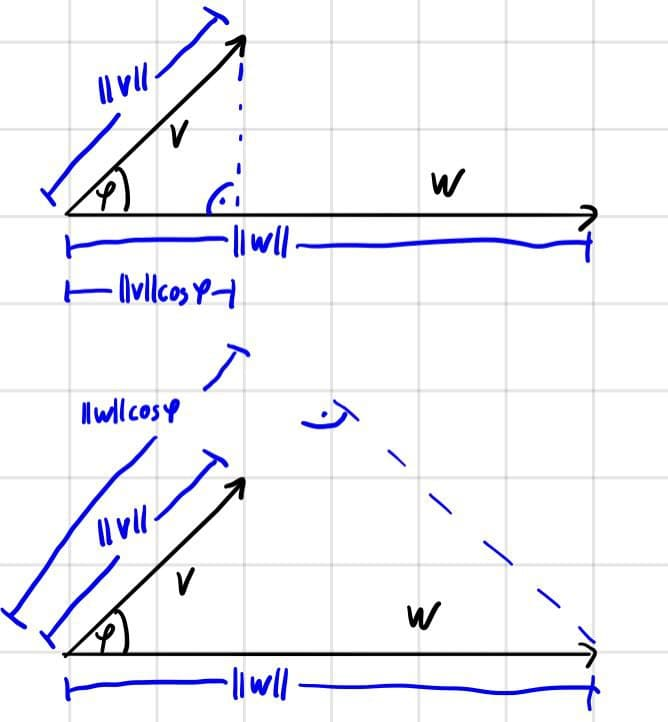
\includegraphics[width=.25\textwidth]{Dateien/04/04Skalarprodukt.jpg}
 \vspace{-15pt}
\end{wrapfigure}
Wir hatten den Winkel zweier Vektoren $\vvec,\wvec\in V\setminus\MengeDirekt{\Vec{0}}$\footnote{wobei $V$ ein euklidischer VR, d.h. ein VR mit einem Skalarprodukt ist} als
\begin{equation*}
    \angle(\vvec,\wvec):=\arccos\frac{\BiFo{\vvec,\wvec}}{\Norm{\vvec}\cdot\Norm{\wvec}}\in[0,\pi]
\end{equation*}
definiert, was anders aufgeschrieben $\BiFo{\vvec,\wvec}=\Norm{\vvec}\cdot\Norm{\wvec}\cos\varphi$ ist.\\
\blue{Das Skalarprodukt multipliziert also die Längen der Vektoren und berücksichtigt dabei den eingeschlossenen Winkel.\\
Tatsächlich ist es die Projektion der Vektoren $\vvec$ und $\wvec$ aufeinander, die multipliziert wird (siehe Skizze).}
\end{Wiederholung}
\blue{Mit dieser Erklärung wird vielleicht auch klar, weshalb $\BiFo{\vvec,\wvec}=0\iff \vvec\perp \wvec$ und\\
$\Abs{\BiFo{\vvec,\wvec}}=\Norm{\vvec}\cdot\Norm{\wvec}\iff \vvec,\wvec$ linear abhängig.}
\newpage
Bei dem gleich folgenden Verfahren ist es nützlich, im Kopf zu haben, was die verschiedenen Operationen von Vektoren anschaulich im $\mathbb{R}^2$ bedeuten:
\begin{Wiederholung}
{Addition und Subtraktion von Vektoren im $\mathbb{R}^2$}
\begin{wrapfigure}{r}[0pt]{.15\textwidth}
 \vspace{-15pt}
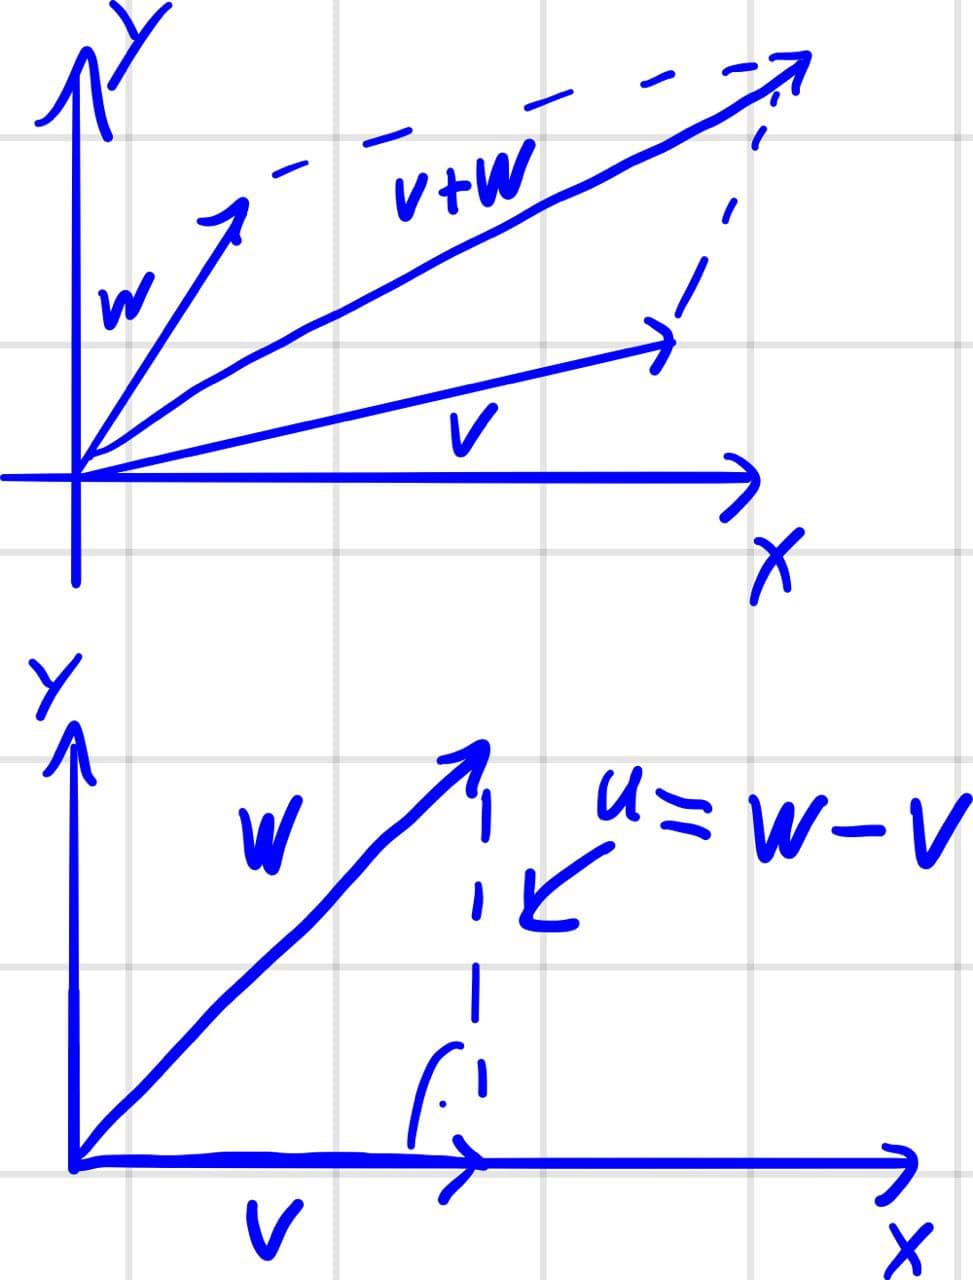
\includegraphics[width=.15\textwidth]{Dateien/04/04Vektoraddition.jpg}
 \vspace{-15pt}
\end{wrapfigure}
Geometrisch kann im $\mathbb{R}^2$ die Summe zweier Vektoren gewonnen werden, indem ein Parallelogramm gezeichnet wird.\\
Somit ist die Differenz zweier Vektoren quasi die dritte Seite eines Dreiecks.\\
Falls wir also wissen, dass $\vvec$ die orthogonale Projektion\footnote{welche wir mithilfe des Skalarprodukts gewinnen können} von $\wvec$ auf die bisherige Basis ist, erhalten wir durch $\vvec+\uvec=\wvec\iff \uvec=\wvec-\vvec$ einen zu $\vvec$ orthogonalen Vektor (siehe Skizze).
\end{Wiederholung}
\begin{Satz}{Kochrezept}{Gram-Schmidt-Verfahren}
\blue{Wir starten mit einer vorgegebenen Basis $B=(\textcolor{blue}{\vvec_1},\textcolor{blue}{\vvec_2},\ldots,\vvec_n)$ in einem euklidischen Vektorraum mit vorgegebenen Skalarprodukt.}\\
\red{Das Ziel ist eine orthonormale Basis $B'=(\textcolor{red}{\wvec_1},\textcolor{red}{\wvec_2},\ldots,\textcolor{red}{\wvec_n})$.}\\
So gehen wir vor:
\begin{enumerate}
	\item Wir fangen mit einem beliebigen Vektor, z. B. $\textcolor{blue}{\vvec_1}$, aus $B$ an und normieren diesen. Das ist schon der erste Vektor der neuen Basis:
	\begin{equation}
	\boxed{\textcolor{red}{\wvec_1}=\frac{\textcolor{blue}{\vvec_1}}{\Norm{\textcolor{blue}{\vvec_1}}}}.
	\end{equation}
	\item Falls die Basis $B'$ an dieser Stelle\footnote{Da man häufig zu diesem Schritt zurückkommt, tun wir so, als hätten wir schon $k$ orthonormale Basisvektoren gefunden. Das ist vielleicht anfangs ein wenig verwirrend, aber ergibt nach Schritt 5 mehr Sinn. Im Zweifel könnt ihr zunächst einfach $k=1$ betrachten :)} noch nicht orthogonal ist, konstruieren wir die \underline{orthogonale Projektion} $\textcolor{orange}{\Tilde{\vvec}_{k+1}}$ aus den bisher gewonnenen Basisvektoren $(\textcolor{red}{\wvec_1},\ldots,\textcolor{red}{\wvec_k})$ und dem nächsten Vektor $\vvec_{k+1}$ aus $B$:
	\begin{equation}
		\boxed{\textcolor{orange}{\Tilde{\vvec}_{k+1}}=\BiFo{\textcolor{blue}{\vvec_{k+1}},\textcolor{red}{\wvec_1}}\textcolor{red}{\wvec_1}+\ldots+\BiFo{\textcolor{blue}{\vvec_{k+1}},\textcolor{red}{\wvec_k}}\textcolor{red}{\wvec_k}}.
	\end{equation}
	Für den zweiten Basisvektor ist dies einfach
	\begin{equation*}
	    \textcolor{orange}{\Tilde{\vvec}_2}=\BiFo{\textcolor{blue}{\vvec_2},\textcolor{red}{\wvec_1}}\textcolor{red}{\wvec_1}.
	\end{equation*}
	\item Durch Subtraktion kann nun die Richtung des nächsten Basisvektors ermittelt werden, da so alle bisherigen Komponenten der Basis abgezogen werden:
	\begin{equation}
		\boxed{\textcolor{mygreen}{\Tilde{\wvec}_{k+1}}=\textcolor{blue}{\vvec_{k+1}}-\textcolor{orange}{\Tilde{\vvec}_{k+1}}}.
	\end{equation}
	Für den zweiten Basisvektor ist dies einfach
	\begin{equation*}
	    \textcolor{mygreen}{\Tilde{\wvec}_2}=\textcolor{blue}{\vvec_2}-\textcolor{orange}{\Tilde{\vvec}_2}.
	\end{equation*}
	\item Nun müssen wir diesen nur noch Normieren:
	\begin{equation}
	    \boxed{\textcolor{red}{\wvec_{k+1}}=\frac{\textcolor{mygreen}{\Tilde{\wvec}_{k+1}}}{\Norm{\textcolor{mygreen}{\Tilde{\wvec}_{k+1}}}}}.
	\end{equation}
	Für den zweiten Basisvektor ist dies einfach
	\begin{equation*}
	\textcolor{red}{\wvec_{2}}=\frac{\textcolor{mygreen}{\Tilde{\wvec}_{2}}}{\Norm{\textcolor{mygreen}{\Tilde{\wvec}_{2}}}}.
	\end{equation*}
	\item Nun müsst ihr die Schritte 2 bis 5 für den nächsten Vektor aus $B$ wiederholen, bis $B'$ vollständig orthonormal ist, ihr also alle $\textcolor{blue}{\vvec_i}$ verarbeitet habt.
\end{enumerate}
\end{Satz}
\begin{center}
    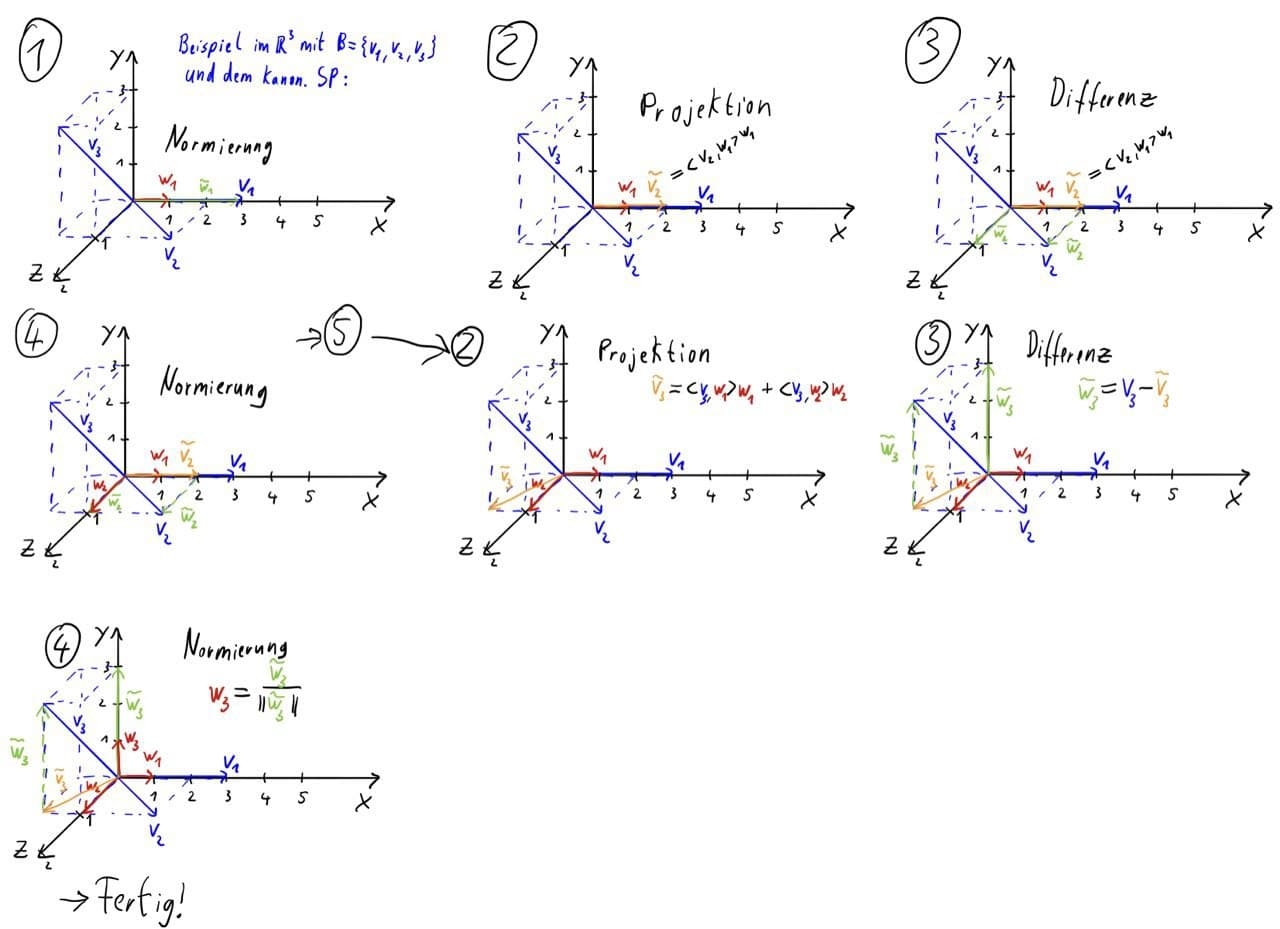
\includegraphics[width=\textwidth]{Dateien/03/03GramSchmidt.jpg}
\end{center}
In diesem Schaubild haben wir versucht, das Gram-Schmidt-Verfahren im $\mathbb{R}^3$ anschaulich darzustellen.

\begin{Beispiel}
{Anwendung des Gram-Schmidt-Verfahrens (1/2)}
Wir betrachten den $\mathbb{R}^3$ dem folgenden euklidischen Skalarprodukt:
\begin{equation*}
    \delta:\mathbb{R}^3\times \mathbb{R}^3\to\mathbb{R},\\
    \delta(\xvec,\yvec):=\BiFo{\xvec,\yvec}=4x_1y_1-2x_1y_2-2x_2y_1+4x_2y_2+x_3y_3+ x_3y_2+x_2y_3.
\end{equation*}
Bezüglich der kanonischen Basis $\hat{B}$ ist die darstellende Matrix dann
\begin{equation*}
    \Delta:=\Matrix{4&-2&0\\-2&4&1\\0&1&1}.
\end{equation*}
\blue{Wir sehen auch direkt, dass die Matrix symmetrisch ist. Tatsächlich ist sie auch positiv definit.\footnote{Es gibt Methoden, dies aus der Matrix abzulesen. Darauf möchten wir hier aber nicht eingehen. Es reicht nicht, dass $\det A>0$ ist! Dies ist aber trotzdem ein notwendiges Kriterium.}}\\
Wie würde nun eine ONB bezüglich dieses Skalarproduktes aussehen?\\
Wir fangen mit der kanonischen Basis $\hat{B}=\MengeDirekt{\MatrixInline{1\\0\\0},\MatrixInline{0\\1\\0},\MatrixInline{0\\0\\1}}=:\MengeDirekt{\textcolor{blue}{\vvec_1},\textcolor{blue}{\vvec_2},\textcolor{blue}{\vvec_3}}$ an und wählen $\textcolor{blue}{\vvec_1}$ als ersten Vektor:
\begin{enumerate}
    \item Die Länge von $\textcolor{blue}{\vvec_1}$ müssen wir nun\footnote{wahrscheinlich recht ungewohnt} bzgl. $\delta$ bestimmen, wir haben also
    \begin{equation*}
        \Norm{\textcolor{blue}{\vvec_1}}=\sqrt{\BiFo{\textcolor{blue}{\vvec_1},\textcolor{blue}{\vvec_1}}}=\sqrt{\Matrix{1&0&0}\Matrix{4&-2&0\\-2&4&1\\0&1&1}\Matrix{1\\0\\0}}=\sqrt{4}=2.
    \end{equation*}
    \red{Die Länge des kanonischen Einheitsvektors ist also bzgl. dieses Skalarproduktes nicht 1!}\\
    Somit legen wir fest:
    \begin{equation*}
        \textcolor{red}{\wvec_1}=\frac{\textcolor{blue}{\vvec_1}}{\Norm{\textcolor{blue}{\vvec_1}}}=\frac{1}{2}\Matrix{1\\0\\0}.
    \end{equation*}
    \item Wir projizieren $\textcolor{blue}{\vvec_2}$ auf $\textcolor{red}{\wvec_1}$:
    \begin{align*}
        \textcolor{orange}{\Tilde{\vvec}_2}&=\BiFo{\textcolor{blue}{\vvec_2},\textcolor{red}{\wvec_1}}\textcolor{red}{\wvec_1}=\Matrix{0&1&0}\Matrix{4&-2&0\\-2&4&1\\0&1&1}\Matrix{1/2\\0\\0}\textcolor{red}{\wvec_1}\\
        &=\Matrix{0&1&0}\Matrix{2\\-1\\0}\textcolor{red}{\wvec_1}=-1\textcolor{red}{\wvec_1}
    \end{align*}
    \item Wir ziehen die bisherigen Basiskomponenten ab:
    \begin{equation*}
        \textcolor{mygreen}{\Tilde{\wvec}_2}=\textcolor{blue}{\vvec_2}-\textcolor{orange}{\Tilde{\vvec}_2}=\Matrix{0\\1\\0}-\BracedIn{-\frac{1}{2}}\Matrix{1\\0\\0}=\Matrix{1/2\\1\\0}.
    \end{equation*}
    \item Abschließend normieren wir:
    \begin{align*}
        \Norm{\textcolor{mygreen}{\Tilde{\wvec}_2}}&=\sqrt{\Matrix{1/2&1&0}\Matrix{4&-2&0\\-2&4&1\\0&1&1}\Matrix{1/2\\1\\0}}=\sqrt{\Matrix{1/2&1&0}\Matrix{0\\3\\0}}=\sqrt{3}\\
        \implies \textcolor{red}{\wvec_2}&=\frac{\textcolor{mygreen}{\Tilde{\wvec}_2}}{\Norm{\textcolor{mygreen}{\Tilde{\wvec}_2}}}=\frac{1}{2\sqrt{3}}\Matrix{1\\2\\0}.
    \end{align*}
    \item Weil wir noch nicht alle Basisvektoren verarztet haben, kehren wir mit $\textcolor{blue}{\vvec_3}$ zu Schritt 2 zurück:\setcounter{enumi}{1}
    \item Wir projizieren $\textcolor{blue}{\vvec_3}$ auf die bisher gefundenen Basisvektoren $\textcolor{red}{\wvec_1}$ und $\textcolor{red}{\wvec_2}$:\footnote{Nebenrechnung: $\BiFo{\textcolor{blue}{\vvec_3},\textcolor{red}{\wvec_1}}=\textcolor{blue}{\vvec_3}^T \Delta \textcolor{red}{\wvec_1}=0$ und $\BiFo{\textcolor{blue}{\vvec_3},\textcolor{red}{\wvec_2}}=\textcolor{blue}{\vvec_3}^T\Delta \textcolor{red}{\wvec_2}=\frac{1}{2\sqrt{3}}\Matrix{0&0&1}\Matrix{0\\6\\2}=\frac{1}{\sqrt{3}}$.}
    \begin{equation*}
        \textcolor{orange}{\Tilde{\vvec}_3}=\BiFo{\textcolor{blue}{\vvec_3},\textcolor{red}{\wvec_1}}\textcolor{red}{\wvec_1}+\BiFo{\textcolor{blue}{\vvec_3},\textcolor{red}{\wvec_2}}\textcolor{red}{\wvec_2}=0\textcolor{red}{\wvec_1}+\frac{1}{\sqrt{3}}\textcolor{red}{\wvec_2}.
    \end{equation*}
    \item Wir ziehen die Projektion von $\textcolor{blue}{\vvec_3}$ ab:
    \begin{equation*}
        \textcolor{mygreen}{\Tilde{\wvec}_3}=\textcolor{blue}{\vvec_3}-\textcolor{orange}{\Tilde{\vvec}_3}=\Matrix{0\\0\\1}-\frac{1}{\sqrt{3}}\frac{1}{2\sqrt{3}}\Matrix{1\\2\\0}=\Matrix{-1/6\\-2/6\\1}=\frac{1}{6}\Matrix{-1\\-2\\6}.
    \end{equation*}
    \item Abschließend normieren wir:
    \begin{align*}
        \Norm{\textcolor{mygreen}{\Tilde{\wvec}_3}}&=\sqrt{\textcolor{mygreen}{\Tilde{\wvec}_3}^T\Delta \textcolor{mygreen}{\Tilde{\wvec}_3}}=\frac{1}{6}\sqrt{\Matrix{-1&-2&6}\Matrix{0\\-6\\4}}=\frac{1}{6}36=6\\
    \implies \textcolor{red}{\wvec_3}&=\frac{\textcolor{mygreen}{\Tilde{\wvec}_3}}{\Norm{\textcolor{mygreen}{\Tilde{\wvec}_3}}}=\frac{1}{36}\Matrix{-1\\-2\\6}.  
    \end{align*}
\end{enumerate}
Bezüglich des $\delta$-Skalarproduktes ist also $B'=\MengeDirekt{\frac{1}{2}\MatrixInline{1\\0\\0},\frac{1}{2\sqrt{3}}\MatrixInline{1\\2\\0},\\\frac{1}{36}\MatrixInline{-1\\-2\\6}}$ eine Orthonormalbasis!
\end{Beispiel}

\begin{Beispiel}
{Anwendung des Gram-Schmidt-Verfahrens (2/2)}
Wir suchen erneut eine orthogonale Basis bzgl. eines exotischen Skalarproduktes:
Für $\xvec,\yvec\in\mathbb{R}^3$ definieren wir das Skalarprodukt
\begin{equation*}
    \BiFo{\xvec,\yvec}=x_1y_1+2x_2y_2+3x_3y_3-x_2y_1-x_1y_2.
\end{equation*}
Wir beginnen mit der Basis $B:=\MengeDirekt{\MatrixInline{1\\1\\0},\MatrixInline{0\\1\\0},\MatrixInline{0\\0\\1}}=\MengeDirekt{\textcolor{blue}{\bvec_1},\textcolor{blue}{\bvec_2},\textcolor{blue}{\bvec_3}}$ und fordern, dass $\textcolor{blue}{\bvec_1}$ normiert in $B'$ enthalten ist.\\
Um uns das Leben leichter zu machen, stellen wir zunächst die darstellende Matrix $A$ von $\BiFo{\cdot,\cdot}$ bzgl. der kanonischen Basis auf:
\begin{equation*}
    A=\Matrix{1&-1&0\\-1&2&0\\0&0&3}.
\end{equation*}
Diese Matrix ist symmetrisch und positiv definit.
\begin{enumerate}
    \item Die Länge von $\textcolor{blue}{\bvec_1}$ ist
    \begin{align*}
        \Norm{\textcolor{blue}{\bvec_1}}&=\sqrt{\BiFo{\textcolor{blue}{\bvec_1},\textcolor{blue}{\bvec_1}}}=\sqrt{\textcolor{blue}{\bvec_1}^TA\textcolor{blue}{\bvec_1}}\\
        &=\sqrt{\Matrix{1&1&0}\Matrix{1&-1&0\\-1&2&0\\0&0&3}\Matrix{1\\1\\0}}=\sqrt{\Matrix{1&1&0}\Matrix{0&1&0}}=1.
    \end{align*}
    Somit legen wir fest:
    \begin{equation*}
        \textcolor{red}{\wvec_1}=\frac{\textcolor{blue}{\bvec_1}}{\Norm{\textcolor{blue}{\bvec_1}}}=\Matrix{1\\1\\0}.
    \end{equation*}
    \item Wir projizieren $\textcolor{blue}{\bvec_2}$ auf $\textcolor{red}{\wvec_1}$:
    \begin{equation*}
        \textcolor{orange}{\Tilde{b}_2}=\BiFo{\textcolor{blue}{\bvec_2},\textcolor{red}{\wvec_1}}\textcolor{red}{\wvec_1}=(\textcolor{blue}{\bvec_2}^T A \textcolor{red}{\wvec_1})\textcolor{red}{\wvec_1}=\Matrix{1\\1\\0}.
    \end{equation*}
    \item Wir ziehen die bisherigen Basiskomponenten ab:
    \begin{equation*}
        \textcolor{mygreen}{\Tilde{\wvec}_2}=\textcolor{blue}{\bvec_2}-\textcolor{orange}{\Tilde{b}_2}=\Matrix{-1\\0\\0}.
    \end{equation*}
    \item Abschließend normieren wir:\footnote{Es ist $\Norm{\textcolor{mygreen}{\Tilde{\wvec}_2}}=1$.}
    \begin{equation*}
        \textcolor{red}{\wvec_2}=\frac{\textcolor{mygreen}{\Tilde{\wvec}_2}}{\Norm{\textcolor{mygreen}{\Tilde{\wvec}_2}}}=\Matrix{-1\\0\\0}.
    \end{equation*}
    \item Weil wir noch nicht alle Basisvektoren verarztet haben, kehren wir mit $\textcolor{blue}{\vvec_3}$ zu Schritt 2 zurück:\setcounter{enumi}{1}
    \item Wir projizieren $\textcolor{blue}{\bvec_3}$ auf die bisher gefundenen Basisvektoren $\textcolor{red}{\wvec_1}$ und $\textcolor{red}{\wvec_2}$:\footnote{Nebenrechnung: $\BiFo{\textcolor{blue}{\bvec_3},\textcolor{red}{\wvec_1}}=\textcolor{blue}{\bvec_3}^T \Delta \textcolor{red}{\wvec_1}=0$ und $\BiFo{\textcolor{blue}{\bvec_3},\textcolor{red}{\wvec_2}}=0$.}
    \begin{equation*}
        \textcolor{orange}{\Tilde{b}_3}=\Matrix{0\\0\\0}.
    \end{equation*}
    \item Wir ziehen die Projektion von $\textcolor{blue}{\bvec_3}$ ab:
    \begin{equation*}
        \textcolor{mygreen}{\Tilde{\wvec}_3}=\textcolor{blue}{\bvec_3}-\textcolor{orange}{\Tilde{b}_3}=\Matrix{0\\0\\1}.
    \end{equation*}
    \item Abschließend normieren wir:
    \begin{align*}
        \Norm{\textcolor{mygreen}{\Tilde{\wvec}_3}}&=\sqrt{\textcolor{mygreen}{\Tilde{\wvec}_3}^T\Delta \textcolor{mygreen}{\Tilde{\wvec}_3}}=3\\
    \implies \textcolor{red}{\wvec_3}&=\frac{1}{3}\Matrix{0\\0\\1}.
    \end{align*}
\end{enumerate}
\end{Beispiel}

\subsection{Hermitesche Formen: Bilinearformen in komplex}
\blue{In diesem Kapitel werdet ihr oft den Satz 'Analog zu euklidischen Vektorräumen definieren wir...' finden, aber es gibt ein paar Feinheiten.\\
Wir erweitern zunächst das Konzept der Bilinearform auf komplexe Vektorräume:}
\begin{Def}
{Hermitesche Form}
Wir nennen\footnote{auf einem komplexen Vektorraum $V$} eine Abbildung $\BiFo{\cdot,\cdot}:V\times V\to\mathbb{C}$ \red{hermitesch} bzw. eine \red{hermitesche Form}, wenn sie $\mathbb{C}$-linear im ersten Argument ist und zudem $\forall \vvec,\wvec\in V$ gilt:
\begin{equation}
    \boxed{\overline{\BiFo{\vvec,\wvec}}=\BiFo{\wvec,\vvec}}.
\end{equation}
\blue{Sie muss also eine Art \textit{komplexe Symmetrie} erfüllen.}
\end{Def}
Folgende Definition liegt für komplexe Vektorräume auf der Hand:
\begin{Def}
{Konjugierte Linearität}
Eine Abbildung $F:V\to W$ zwischen komplexen Vektorräumen heißt \red{konjugiert linear}, wenn
\begin{equation}
    F(\vvec+\wvec)=F(\vvec)+F(\wvec)\quad\tx{und}\quad F(\lambda \vvec)=\overline{\lambda}F(\vvec)\quad\forall \vvec, \wvec\in V,\,\forall\lambda\in \mathbb{C}.
\end{equation}
\end{Def}
\blue{Aus der Linearität im ersten Argument und der Symmetriebedingung folgt, dass hermitesche Formen konjugiert linear im zweiten Argument sind: $\forall \uvec,\vvec,\wvec\in V,\lambda\in\mathbb{C}$ gilt:
\begin{equation*}
    \BiFo{\uvec,\lambda \vvec+\wvec}\overset{\footnotemark}{=}\overline{\lambda}\BiFo{\uvec,\vvec}+\BiFo{\uvec,\wvec}.
\end{equation*}\footnotetext{Denn $\BiFo{\uvec,\lambda \vvec+\wvec}=\overline{\BiFo{\lambda \vvec+\wvec, \uvec}}=\overline{\lambda\BiFo{\vvec,\uvec}+\BiFo{\wvec,\uvec}}=\overline{\lambda}\BiFo{\uvec,\vvec}+\BiFo{\uvec,\wvec}$, wobei wir die komplexe Symmetrie und die Linearität im 1. Argument genutzt haben.}Zudem ist $\BiFo{\vvec,\vvec}\in\mathbb{R}\,\forall \vvec\in V$, weil $\BiFo{\vvec,\vvec}\overset{!}{=}\overline{\BiFo{\vvec,\vvec}}\implies \Im (\BiFo{\vvec,\vvec})=0$.}
\subsubsection{Komplexere Skalarprodukte}
Wie auch für das euklidische SP fordern wir noch die positive Definitheit für hermitesche SP. Diese ist wie folgt definiert:
\begin{Def}
{Positive Definitheit (Hermitesche Formen)}
Weil $\BiFo{\vvec,\vvec}$ reell ist, können wir die Ordnungsrelationen verwenden und analog zu Bilinearformen die \red{positive Definitheit} von hermiteschen Formen definieren:
\begin{equation}
    \BiFo{\cdot,\cdot}\tx{ pos. definit}\iff \BiFo{\vvec,\vvec}>0\quad\forall \vvec\in V\setminus\MengeDirekt{\Vec{0}}.
\end{equation}
\end{Def}
\begin{Def}
{Hermitesches Skalarprodukt}
Eine \underline{positiv definite hermitesche Form} $\BiFo{\cdot,\cdot}: V\times V\to \mathbb{C}$ nennen wir \red{hermitesches Skalarprodukt}.
\end{Def}
\begin{Def}
{Hermitescher Vektorraum}
Einen komplexen Vektorraum nennen wir \red{hermitesch} oder auch \red{unitär}, falls für ihn ein hermitesches Skalarprodukt definiert ist.
\end{Def}
\begin{Beispiel}
{Kanonisches Skalarprodukt}
Auf $\mathbb{C}^n$ ist durch $\BiFo{\cdot,\cdot}:\mathbb{C}^n\times \mathbb{C}^n\to\mathbb{C},\,(\vvec,\wvec)\mapsto \BiFo{\vvec,\wvec}=\sum_{i=1}^n\vvec_i\overline{\wvec_i}$ das kanonische hermitesche Skalarprodukt definiert.
\end{Beispiel}

\begin{Def}
{Norm von Vektoren und die Cauchy-Schwarzsche Ungleichung}
Analog zu euklidischen Vektorräumen definieren wir die \red{Norm} bzw. \red{Länge} eines Vektors $v\in V$ (wobei $V$ ein herm. VR ist) als
\begin{equation}
    \Norm{\vvec}:=\sqrt{\BiFo{\vvec,\vvec}}
\end{equation}
und es gilt
\begin{equation}
    \Abs{\BiFo{\vvec,\wvec}}\leq \Norm{\vvec}\cdot\Norm{\wvec}\quad \forall \vvec,\wvec\in V.
\end{equation}
\end{Def}

\subsubsection{Unitarität ist die komplexe Orthogonalität}
\begin{Def}
{Unitäre Basis}
Analog zur orthogonalen Basis für euklidische Vektorräume nennen wir die Basis $B$ eines herm. Vektorraums $V$ \red{unitär}, wenn
\begin{equation}
\BiFo{\wvec_i,\wvec_j}=\delta_{ij}\quad\forall \wvec_i, \wvec_j\in B.
\end{equation}
\end{Def}
\begin{Satz}
{Satz}{Existenz einer unitären Basis}
Auch hier kann man zeigen, dass jeder hermitesche Vektorraum eine Basis besitzt.
\end{Satz}

\subsection{Klassifikation von Endomorphismen}
\blue{Wir betrachten nun wieder Endomorphismen\footnote{diesmal auf euklidischen oder hermiteschen Vektorräumen} und schauen uns Eigenschaften an, die wir mithilfe eines Skalarproduktes überprüfen können.}

\subsubsection{Orthogonale und unitäre Endomorphismen}
\blue{Die ersten Kandidaten dafür sind Abbildungen, welche Winkelbeziehungen, Längen und Abstände von Vektoren erhalten:}
\begin{Def}
{Orthogonale Endomorphismen}
Auf einem euklidischen Vektorraum $V,\BiFo{\cdot,\cdot})$ nennen wir eine \underline{surjektive} lineare Abbildung $F:V\to V$ \red{orthogonal}, wenn gilt
\begin{equation}
    \boxed{\BiFo{F(\vvec),F(\wvec)}=\BiFo{\vvec,\wvec}}\quad \forall \vvec,\wvec\in V.
\end{equation}
\end{Def}
\blue{Aufgrund der Bedingung ist $F$ \underline{stets injektiv}, denn\\ $F(\vvec)=0\implies \vvec=0$, weil ja $0=\BiFo{F(\vvec),F(\vvec)}=\BiFo{\vvec,\vvec}$.\\
Auf endlichdimensionalen Vektorräumen ist $F$ aufgrund der Dimensionsformel dann auch surjektiv. So oder so ist $F$ stets ein \underline{bijektiver Endomorphismus}, was wir ja auch als \underline{Automorphismus} bezeichnen.}
\begin{Def}
{Orthogonale Gruppe}
Es gilt: $O(V)\subseteq \Aut(V)$, d. h. die \red{orthogonale Gruppe\footnote{diese beinhaltet alle orthogonalen Endomorphismen von $V$} $O(V)$} ist eine Untergruppe der Automorphismen.
\end{Def}
\begin{Satz}
{Satz}{Matrizen orthogonaler Endomorphismen im $\mathbb{R}^n$}
Im $\mathbb{R}^n$ gilt mit dem kanonischen Skalarprodukt, dass $O(n):=O(\mathbb{R}^n,\BiFo{\cdot,\cdot})$ der Gruppe \red{invertierbarer Matrizen} entspricht, für die
\begin{equation}
    A^{-1}=A^T \iff A^T A=\mathds{1}_n.
\end{equation}
\end{Satz}
\begin{Def}
{Unitäre Endomorphismen}
Analog dazu bezeichnet man surjektive lineare Abbildungen $F:V\to V$ auf hermiteschen Vektorräumen $V$ als \red{unitär}, wenn
\begin{equation}
    \boxed{\BiFo{F(\vvec),F(\wvec)}=\BiFo{\vvec,\wvec}}\quad \forall \vvec,\wvec\in V.
\end{equation}
\end{Def}
\blue{Auch hier folgt wieder die Injektivität direkt und die Surjektivität muss für $\dim V<\infty$ nicht gefordert werden. Die \red{unitäre Gruppe} ist ebenfalls eine Untergruppe der Automorphismen, $U(V)\subseteq \Aut(V)$.}
\begin{Def}
{Notation: $A$ Dagger}
Wir definieren das gleichzeitige komplexe Konjugieren und Transponieren einer Matrix $A\in\mathbb{C}^n$ mit dem folgenden Zeichen: $A^\dag:=\overline{A}^T=\overline{A^T}$ (sprich: 'A dagger').
\end{Def}
\begin{Satz}
{Matrizen unitärer Endomorphismen im $\mathbb{C}^n$}
Im $\mathbb{C}^n$ gilt mit dem kanonischen Skalarprodukt $\BiFo{\wvec,\zvec}=\sum_{i=1}^nw_i\overline{z_i}$, dass $U(n):=U(\mathbb{C}^n,\BiFo{\cdot,\cdot})$ der Gruppe \red{invertierbarer Matrizen} entspricht, für die
\begin{equation}
    A^{-1}=A^\dag \iff A^\dag A=\mathds{1}_n.
\end{equation}
\end{Satz}
Unitäre Matrizen sind in der Physik unglaublich wichtig - z. B. lernt ihr in Physik 5 die \href{https://de.wikipedia.org/wiki/CKM-Matrix}{CKM-Matrix} kennen, die essenzieller Bestandteil des heutigen Standardmodells der Teilchenphysik ist.\\
Ein anschauliches Beispiel ist die euch bekannte Drehmatrix:
\begin{Beispiel}
{Drehmatrix}
Im $\mathbb{R}^2$ ist die Drehmatrix $D_\varphi=\MatrixInline{\cos\varphi&-\sin\varphi\\\sin\varphi&\cos\varphi}$ ein orthogonaler Endomorphismus, denn es gilt
\begin{align*}
    D_\varphi^TD_\varphi&=\Matrix{\cos\varphi&\sin\varphi\\-\sin\varphi&\cos\varphi}\Matrix{\cos\varphi&-\sin\varphi\\\sin\varphi&\cos\varphi}\\
    &=\Matrix{\cos^2\varphi-(-\sin^2\varphi)&\cos\varphi\sin\varphi-\cos\varphi\sin\varphi\\0&\cos^2\varphi+\sin^2\varphi}=\Matrix{1&0\\0&1}=\mathds{1}_2.
\end{align*}
\textbf{Alternativer Beweis}:\\
Für $\vvec,\wvec\in\mathbb{R}^2,\vvec:=\MatrixInline{a\\b}, \wvec:=\MatrixInline{c\\d}$ gilt
\begin{align*}
    \BiFo{D_\varphi \vvec,D_\varphi \wvec}&=\BiFo{\Matrix{a\cos\varphi-b\sin\varphi\\a\sin\varphi+b\cos\varphi},\Matrix{c\cos\varphi-d\sin\varphi\\c\sin\varphi+d\cos\varphi}}\\
    &=ac\cos\varphi^2-ad\cos\varphi\sin\varphi-bc\cos\varphi\sin\varphi+bd\sin\varphi^2+ac\cos\varphi^2\\
    &\quad +ad\cos\varphi\sin\varphi+bc\cos\varphi\sin\varphi+bd\sin\varphi^2\\
    &=ac(\cos^2\varphi+\sin^2\varphi)+bd(\sin^2\varphi+\cos^2\varphi)=ac+bd\\
    &=\BiFo{\Matrix{a\\b},\Matrix{c\\d}}=\BiFo{\vvec,\wvec}.
\end{align*}
\end{Beispiel}

\subsubsection{Diagonalisierung orthogonaler/unitärer Endomorphismen}
Die darstellenden Matrizen orthogonaler bzw. unitärer Endomorphismen sind in besonderer Weise diagonalisierbar.\\
Aufgrund der Eigenschaft, Längen von Vektoren zu erhalten, haben die Eigenwerte stets den Betrag 1.\footnote{Kurze Übungsaufgabe: Könnt ihr zeigen, dass für unitäre Matrizen $U$ stets $\Abs{\det U}=1$ gilt?\\
Für solche Matrizen ist $U^\dag U=\mathds{1}_n$, woraus folgt, dass $1=\det\mathds{1}_n=\det(U^\dag U)=\det U^\dag \det U=\overline{\det U^T}\det U=\Abs{\det U}^2$, wobei wir den Determinantenmultiplikationsatz und $\det A^T=\det A$ genutzt haben.
}
Zudem hat die Basis des Vektorraumes, bzgl. derer diese Diagonalgestalt erreicht wird, besondere Eigenschaften.
\begin{Satz}
{Satz}{Normalform orthogonaler (bzw. unitärer) Endomorphismen}
Auf euklidischen Vektorräumen $V$ mit $\dim V<\infty$ gilt für $F\in O(V)$:
\begin{enumerate}
    \item Eigenwerte von $F$ sind $+1$ oder $-1$.
    \item Eigenvektoren zu verschiedenen Eigenwerten stehen \underline{senkrecht} aufeinander.
    \item Es existiert eine \underline{Orthonormalbasis}, bzgl. derer die darst. Matrix $A_F$ die folgende Gestalt annimmt:
    \begin{equation}
        A_F=\diag\BracedIn{\lambda_1,\ldots,\lambda_p,D_{\varphi_1},\ldots,D_{\varphi_q}}
    \end{equation}
    mit $\lambda_j\in\MengeDirekt{-1,1}$ und $D_{\varphi_j}=\MatrixInline{\cos\varphi_j&-\sin\varphi_j\\\sin\varphi_j&\cos\varphi_j}$ mit $\phi_j\in\mathbb{R}$.\\
    Hierbei gilt, dass $p+2q=\dim V$.
\end{enumerate}
Auf hermiteschen, endlichdimensionalen Vektorräumen gilt analog für $F\in U(V)$:
\begin{enumerate}
    \item Eigenwerte $\lambda_i$ sind komplexe Zahlen mit $\Abs{\lambda_i}=1$.
    \item Eigenvektoren zu verschiedenen Eigenwerten sind unitär.
    \item Es existiert eine unitäre Basis, bzgl. derer $A_F$ die folgende Gestalt hat:
    \begin{equation}
        A_F=\diag(\lambda_1,...\lambda_n).
    \end{equation}
    Hier werden die $D_{\varphi_j}$ also nicht benötigt.
\end{enumerate}
\blue{Im komplexen ist $F$ bzgl. einer unitären Basis also komplett diagonalisierbar!}
\end{Satz}
Dass Eigenwerte den Betrag 1 haben müssen, ist mit der Eigenwertgleichung $F(\vvec)=\lambda \vvec$ leicht zu zeigen! Los, probiert es selbst!\\
\Zb{Aufgrund der positiven Definitheit wissen wir,\footnote{egal ob wir euklidische oder hermitesche Vektorräume betrachten} dass $\BiFo{\vvec,\vvec}>0$ für Eigenvektoren von $F$ gilt, da der $\Vec{0}$-Vektor per Definition kein Eigenvektor ist.\\
Es gilt mit der Eigenschaft der orthogonalen/unitären Endomorphismen für Eigenvektoren $\vvec$ von $F$ dann
\begin{equation}
    \BiFo{\vvec,\vvec}\overset{\footnotemark}{=}\BiFo{F(\vvec),F(\vvec)}\overset{\footnotemark}{=}\BiFo{\lambda \vvec,\lambda \vvec}\overset{\footnotemark}{=}\lambda\BiFo{\vvec,\lambda \vvec}=\overset{\footnotemark}{=}\lambda \overline{\lambda}\BiFo{\vvec,\vvec}=\Abs{\lambda}^2\BiFo{\vvec,\vvec}.
\end{equation}\footnotetext{Definition solcher Endomorphismen}\footnotetext{Eigenwert-Gleichung}\footnotetext{Linearität 1. Argument}\footnotetext{Konjugierte Linearität im 2. Argument (für reelle Zahlen ist dies ja egal).}Daraus folgt $1=\Abs{\lambda}^2\implies\Abs{\lambda}=1$.}

\subsubsection{Adjungierte Endomorphismen}
\blue{Wir können das Skalarprodukt auch ausnutzen, um eine weitere lustige Eigenschaft bzw. Beziehung zwischen Endomorphismen zu definieren:}
\begin{Def}
{Adjungiertheit von Endomorphismen}
Für einen Endomorphismus eines eukl. oder herm. Vektorraums $(V,\BiFo{\cdot,\cdot})$ nennen wir $F^\ad\in \End(V)$ den zu $F$ \red{adjungierten} Endomorphismus, wenn
\begin{equation}
    \BiFo{F(\vvec),\wvec}=\BiFo{\vvec,F^\ad(\wvec)}\quad\forall \vvec,\wvec\in V.
\end{equation}
\end{Def}
\begin{Satz}
{Satz}{Eindeutigkeit und Existenz von adj. Endomorphismen}
Es existiert höchstens \underline{ein} $F^\ad$ zu einem gegebenen Endomorphismus $F$.\\
Ist $\dim V<\infty$, so existiert $F^\ad$ für alle $F\in\End(V)$.
\end{Satz}
\begin{Def}
{Selbstadjungiertheite Endomorphismen}
Wir nennen $F\in\End(V)$ \red{selbstadjungiert}, falls $F=F^\ad$, d. h. $\BiFo{F(\vvec),\wvec}=\BiFo{\vvec,F(\wvec)}$ $\forall \vvec,\wvec\in V$.
\end{Def}
\begin{Def}
{Normale Endomorphismen}
Ist die Verknüpfung von $F$ mit $F^\ad$ kommutativ, d. h. $F^\ad\circ F=F\circ F^\ad$, so heißt $F$ \red{normal}.
\end{Def}
\begin{Satz}
{Satz}{Zur darst. Matrix adjungierter Endomorphismen bzgl. Orthonormalbasen}
Auf euklidischen oder hermiteschen Vektorräumen $V$ mit $\dim V<\infty$ ist für $F$ mit darstellender Matrix $A$ bezüglich einer Orthonormalbasis\footnote{bzw. unitären Basis} die darst. Matrix von $F^\ad$ gegeben durch $A^\dagger$.\\
Bzgl. einer solchen Basis gilt also:
\begin{equation}
    F\tx{ selbstadjungiert}\iff A=A^\dag.
\end{equation}
Im komplexen nennen wir eine Matrix $B$ mit $B=B^\dag$ \red{hermitesch}.\footnote{analog zur symmetrischen Matrix mit $B=B^T$.}
\end{Satz}
\blue{\textbf{Anmerkung}:\\
Die darst. Matrizen symmetrischer Bilinearformen bzw. von hermiteschen Formen haben genau diese Eigenschaft.}
\begin{Satz}{Satz}
{Eigenschaften selbstadjungierter Endomorphismen}
Für $F\in\End(V)$ mit $F=F^\ad$ gilt:
\begin{itemize}
    \item $F$ hat reelle Eigenwerte.\\
    \Zb{Sei $v$ ein Eigenvektor zu $\lambda$ mit $\Norm{\vvec}=1$, so ist
    \begin{equation*}
        \lambda=\lambda\BiFo{\vvec,\vvec}\overset{\footnote{Linearität 1. Argument und Eigenwertgleichung}}{=}\BiFo{F(\vvec),\vvec}\overset{\footnote{Selbstadjungiertheit}}{=}\BiFo{\vvec,F(\vvec)}\overset{\footnote{Eigenwertgleichung, konjugierte Linearität im 2. Argument}}{=}\overline{\lambda}\BiFo{\vvec,\vvec}=\overline{\lambda}.
    \end{equation*}}
    \item Eigenvektoren verschiedener Eigenwerte sind paarweise orthogonal.\\
    \Zb{Sei $\lambda$ Eigenwert zum Eigenvektor $\vvec$ und $\mu$ ein dazu verschiedener Eigenwert zum Eigenvektor $\wvec$, so gilt:
    \begin{equation*}
        \lambda\BiFo{\vvec,\wvec}=\BiFo{\lambda \vvec, \wvec}\overset{\footnote{Eigenwertgleichung}}{=}\BiFo{F(\vvec),\wvec}\overset{\footnote{Selbstadjungiertheit}}{=}\BiFo{\vvec,F(\wvec)}\overset{\footnote{Eigenwertgleichung und konjugierte Linearität}}{=}\overline{\mu}\BiFo{\vvec,\wvec}\overset{\footnote{$\mu$ ist reell}}{=}\mu \BiFo{\vvec,\wvec}.
    \end{equation*}
    Da per Voraussetzung $\lambda\neq \mu$, muss $\BiFo{\vvec,\wvec}=0$ sein, d. h. $\vvec\perp \wvec$.}
    \item Für $\dim V<\infty$ existiert stets eine orthogonale bzw. unitäre Basis von $V$, die aus den Eigenvektoren von $F$ besteht.
\end{itemize}
\end{Satz}

\begin{Satz}
{Satz}{Zur Isomophie und Dualisierung}
Für euklidische, endlichdimensionale Vektorräume ist der Raum der symmetrischen Bilinearformen \underline{isomorph}\footnote{d. h., dass eine bijektive lineare Abbildung existiert} zum Raum der selbstadjungierten Endomorphismen. 
\end{Satz}
\blue{Dies ergibt intuitiv auch Sinn, denn wir hatten gesehen, dass darstellende Matrizen symmetrischer Bilinearformen symmetrisch sind, also $A=A^T$. Auf euklidischen Vektorräumen ist dies für Endomorphismen ein Zeichen der Selbstadjungiertheit.}\\
Analog gilt der Satz auch für hermitesche Vektorräume mit hermiteschen Formen.
\subsubsection{Hauptachsentransformation - wenn Endomorphismen Signaturen hinterlassen}
\blue{Durch geschickte Reskalierung der Basisvektoren können wir (weil diese orthogonal sind) eine ganz besondere Form der darstellenden Matrix erhalten, die nur noch von den Vorzeichen der Eigenwerte abhängt.\\
Aufgrund der Isomorphie betrachten wir nun symmetrische Bilinearformen bzw. hermitesche Formen.}
\begin{Satz}
{Satz}{Hauptachsentransformation und Trägheitssatz von Sylvester}
Auf einem euklidischen Vektorraum $V$ mit $\dim V=n$ gilt für \underline{symmetrische} Bilinearformen $\beta$:
\begin{itemize}
    \item Es existiert eine \red{orthogonale Basis} $B=(\bvec_1,\ldots,\bvec_n)$ von $V$, bzgl. derer die darstellende Matrix die folgende Gestalt hat:
    \begin{equation}
        M_B(\beta)=\diag(\mathds{1}_{r_+},-\mathds{1}_{r_-},\Vec{0}_{r_0}).
    \end{equation}
    Hierbei gilt $\boxed{r_++r_-+r_0=n}$ und $\Vec{0}_{r_0}\in\Met(r_0,\mathbb{R})$ die $r_0\times r_0$-Nullmatrix.\\
    Eine solche Gestalt nennt man auch \red{Normalform}.
    \item Die Zahlen $r_+$, $r_-$ und $r_0$ hängen \underline{nicht} von der Wahl der Basis ab.\\
    Man nennt sie auch die \red{Signatur} von $\beta$.
\end{itemize}
Aufgrund der letzten Aussage sind $r_+$ und $r_-$ genau die Anzahl positiver bzw. negativer Eigenwerte.
\end{Satz}
\red{Achtung: $\beta$ muss kein Skalarprodukt sein und ist insbesondere nicht das Skalarprodukt des zugrunde liegenden euklidischen Vektorraums!}
\begin{Beispiel}
{Hauptachsentransformierte Matrix}
Seien $r_+=3$, $r_-=1$, $r_0=2$. Dann ist
\begin{equation*}
    A=\Matrix{1&0&0&0&0&0\\0&1&0&0&0&0\\0&0&1&0&0&0\\0&0&0&-1&0&0\\0&0&0&0&0&0\\0&0&0&0&0&0}
\end{equation*}
die hauptachsentransformierte Matrix auf einem Vektorraum der Dimension\\
$\dim V=3+1+2=6$.
\end{Beispiel}
\begin{Satz}
{Exkurs}{Finden der orthogonalen Basis (nicht im Skript)}\label{satz:04Hauptachsenbasis}
Sei auf einem eukl. VR $V$ eine symmetrische Bilinearform $\beta$ gegeben.\\
Wir suchen nun die orthogonale Basis $B$ von $V$, bzgl. derer die darst. Matrix von $\beta$ Normalform annimmt.\\
Um diese orthogonale Basis zu finden, müssen wir zunächst die Eigenvektoren $\wvec_i$ zu $\beta$ finden. Als Voraussetzung wissen wir ja immerhin, dass diese orthogonal sind.\\
\Zb{Seien $\bvec_i$ die orthogonalen Basisvektoren, die $\beta$ in Normalform bringen, und $\wvec_i$ weiterhin die Eigenvektoren.\\
Da die $\wvec_i$ bereits eine orthogonale Basis bilden, wählen wir $\bvec_i=c_i\wvec_i$ mit $c_i\in\mathbb{R}$, die neuen Basisvektoren müssen also nur noch richtig skaliert werden.\\
Die Frage ist also, wie diese Vorfaktoren gewählt werden müssen.\\
Die Einträge der darstellenden Matrix $\alpha_{ij}$ ergeben sich durch Anwenden der Bilinearform auf die Basisvektoren, $\alpha_{ij}=\beta(\bvec_i,\bvec_j)$.\\
In Normalform haben wir also $N=\MatrixInline{\beta(\bvec_1,\bvec_1)&\cdots& \alpha_{1n}\\\vdots&\ddots&\vdots\\\alpha_{n1}&\cdots&\alpha_{nn}}.$\\
Wir gucken uns das genauer an:
\begin{eqnarray*}
\alpha_{ij}&=&\beta(\bvec_i,\bvec_j)\\
&=&\beta(c_i\wvec_i, c_i\wvec_j)\\
&\overset{\footnote{$\beta$ ist bilinear}}{=}&c_ic_j\beta(\wvec_i,\wvec_j)\\
&\overset{\footnote{$A$ sei die darst. Matrix von $\beta$. Achtung: $\BiFo{\cdot,\cdot}$ ist das Skalarprodukt des eukl. Vektorraums!}}{=}&c_ic_j\BiFo{\wvec_i,A\wvec_j}\\
&\overset{\footnote{Eigenwertgleichung}}{=}&c_ic_j\BiFo{\wvec_i,\lambda_j\wvec_j}\\
&\overset{\footnote{Bilinearität}}{=}&\lambda_jc_ic_j\underbrace{\BiFo{\wvec_i,\wvec_j}}_{=\delta_{ij}\sqrt{\BiFo{\wvec_i,\wvec_j}}^2}\overset{\footnote{weil $\wvec_i$ und $\wvec_j$ als Eigenvektoren einer symmetrischen Bilinearform (isomorph zu selbstadjungierten Endomorphismen) paarweise orthogonal sind.}}{=}\Cases{0&\tx{ wenn } i\neq j\\\lambda_ic_i^2\Norm{\wvec_i}^2&\tx{ wenn } i=j}.
\end{eqnarray*}
Nun sollen aber die Einträge auf der Hauptdiagonalen $\alpha_{ii}$ genau 1, -1 oder 0 sein, also $\Abs{1}$ haben. Für $\lambda_i=0$ stellt sich heraus, dass die Skalierungsfaktoren $c_i$ der $\wvec_i$ egal sind.\\
Für $\lambda_i\neq0$ ergibt sich also:
\begin{equation}
    \sgn(\lambda_i)\cdot 1\overset{!}{=}\lambda_ic_i^2\Norm{\wvec_i}^2\iff \boxed{c_i=\frac{1}{\sqrt{\Abs{\lambda_i}}\Norm{\wvec_i}}}.
\end{equation}
Hierbei nutzten wir das Vorzeichen $\sgn(\lambda_i)$ und den Fakt, dass $\frac{\lambda_i}{\sgn(\lambda_i)}=\Abs{\lambda_i}$ ist. Beim Wurzelziehen haben wir die $c_i$ zudem positiv gewählt, dies ist aber willkürlich.\\
Somit sind die Basisvektoren für die Normalform gegeben durch
\begin{equation*}
    \boxed{\bvec_i=c_i\wvec_i=\Cases{\frac{\wvec_i}{\sqrt{\Abs{\lambda_i}}\Norm{\wvec_i}}&\lambda_i\neq0\\\wvec_i&\lambda_i=0}}.
\end{equation*}}
\end{Satz}

\begin{Satz}
{Satz}{Hauptachsentrafo auf komplexen Vektorräumen}
Für hermitesche Formen $h$ auf $\mathbb{C}$-Vektorräumen existiert ebenfalls eine Basis, bzgl. derer die darst. Matrix von $h$ die Normalform-Gestalt (d. h. $\diag(\mathds{1}_{r_+},-\mathds{1}_{r_-},\Vec{0}_{r_0})$).\\
Hierbei wird (im \Skript{}) aber keine Aussage über die Gestalt der Basis getroffen.\\
Ist $V$ hermitesch, so ist die Basis aber tatsächlich orthogonal.
\end{Satz}

\begin{Beispiel}
{Bestimmung der Signatur und der orthogonalen Basis einer hermiteschen Form}
Wir betrachten
\begin{equation*}
    \gamma:\mathbb{C}^2\times \mathbb{C}^2\to\mathbb{C},\quad \gamma(\vvec,\wvec):=\BiFo{\vvec,\Matrix{2&i\\-i&4}\wvec},
\end{equation*}
wobei $\BiFo{\cdot ,\cdot}$ das kanonische Skalarprodukt von $\mathbb{C}^2$ sei.\\
$\gamma$ ist eine hermitesche Form, denn $A=\MatrixInline{2&i\\-i&4}=\MatrixInline{2&-i\\i&4}^T=\overline{\MatrixInline{2&i\\-i&4}^T}=A^\dag$.\\
Wir suchen die Eigenwerte über das charakteristische Polynom:
\begin{equation*}
    P_A(\lambda)=(2-\lambda)(4-\lambda)+i^2=\lambda^2-6\lambda+7\implies \lambda_1=3+\sqrt{2},\,\lambda_2=3-\sqrt{2}.
\end{equation*}
Weil wir zwei positive Eigenwerte haben, ist die Signatur also\\
$(2,0,0):=r_+=2\land r_-=0\land r_0=0$.\\
Wir suchen nun die Eigenvektoren:
\begin{align*}
    A\wvec_1&=\lambda_1\wvec_1\iff \MatrixInvertieren{-1-\sqrt{2}&i\\-i&1-\sqrt{2}}{0\\0}\to\MatrixInvertieren{1+\sqrt{2}&-i\\1&i(1-\sqrt{2})}{0\\0}\\
    &=\MatrixInvertieren{1+\sqrt{2}&-i\\0&i(1-\sqrt{2})+\frac{i}{1+\sqrt{2}}}{0\\0}=\MatrixInvertieren{1+\sqrt{2}&-i\\0&\frac{i}{1+\sqrt{2}}(1^2-\sqrt{2}^2+1)}{0\\0}\\
    &=\MatrixInvertieren{1+\sqrt{2}&-i\\0&0}{0\\0}\implies y=t\in\mathbb{R}\implies x=\frac{it}{1+\sqrt{2}}
\end{align*}
Somit sind die Eigenvektoren ($\wvec_2$ analog)
\begin{equation*}
    \wvec_1=t\Matrix{\frac{i}{1+\sqrt{2}}\\1},\quad \wvec_2=t\Matrix{\frac{i}{\sqrt{2}-1}\\1}.
\end{equation*}
Diese Eigenvektoren sind orthogonal, denn (wir lassen den Skalierungsfaktor $t$ weg) 
\begin{equation*}
    \BiFo{\wvec_1,\wvec_2}=\sum_{i=1}^2\wvec_{1i}\overline{\wvec_{2i}}=\BracedIn{\frac{i}{1+\sqrt{2}}}\overline{\BracedIn{\frac{i}{\sqrt{2}-1}}}+1=\frac{1}{(1+\sqrt{2})(1-\sqrt{2})}+1=-1+1=0.
\end{equation*}
Wir können nun die unitären Basisvektoren $\bvec_i=\frac{\wvec_i}{\sqrt{\Abs{\lambda_i}}\Norm{\wvec_i}}$ bestimmen:
\begin{align*}
    \Norm{\wvec_1}&=\sqrt{\BiFo{\wvec_1,\wvec_1}}=\sqrt{\frac{i}{1+\sqrt{2}}\frac{-i}{1+\sqrt{2}}t^2+t^2}=t\frac{\sqrt{4+2\sqrt{2}}}{1+\sqrt{2}}=\frac{\sqrt{2(2+\sqrt{2})}(\sqrt{2}-1}{(1+\sqrt{2})(\sqrt{2}-1)}t\\
    &=\frac{\sqrt{2(2+\sqrt{2})(\sqrt{2}-1)(\sqrt{2}-1)}}{2-1}t=\sqrt{2(2-\sqrt{2})}t\\
    \Norm{\wvec_2}&=\sqrt{2(2-\sqrt{2})}t\tx{ analog.}
\end{align*}
Der Faktor $t$ kürzt sich also genau raus, die Basis ist somit
\begin{equation*}
    \wvec_1=\frac{1}{\sqrt{3+\sqrt{2}}}\frac{1}{\sqrt{2(2-\sqrt{2})}}\Matrix{\frac{i}{1+\sqrt{2}}\\1}\quad 
    \wvec_2=\frac{1}{\sqrt{3-\sqrt{2}}}\frac{1}{\sqrt{2(2-\sqrt{2})}}\Matrix{\frac{i}{\sqrt{2}-1}\\1}.
\end{equation*}
Die Form von $\gamma$ bzgl. dieser Basis ist dann $D_\gamma=\MatrixInline{1&0\\0&1}$.
\end{Beispiel}
\blue{Nächste Woche kommen noch weitere Beispiele und eine geometrische Begründung, warum dieses Prozedere überhaupt \textit{Hauptachsentransformation} heißt.}

\Tipps{6}{
\begin{enumerate}
    \item \begin{enumerate}
        \item Einsetzen...
        \item Ein bisschen knobeln, Schaut euch die Gleichungen aus a) an. Die Cauchy-Schwarz'sche Ungleichung kann als Abschätzung sehr gut verwendet werden. Beide Richtungen zeigen!
        \item Nutzt die Bediungung aus a) für $\zvec=\xvec+\yvec$ zeitartig und die reguläre Dreiecksungleichung für $\mathbb{R}$ bzw. $\mathbb{R}^2$.
    \end{enumerate}
    \item Zu dieser Aufgabe werden wir noch ein bisschen vorgestellen.\\
    Was müsst ihr zeigen, um zu begründen, damit $S\in O(4)$?\\
    Die finale Matrixmultiplikation gibt euch dann Gewissheit.
    \item Orientiert euch an eurer letzten Präsenzaufgabe und unseren Beispielen zum Gram-Schmidt-Verfahren.\\
    Verrechnet euch nicht! Über die Orthonormalitätsrelation könnt ihr eure Ergebnisse nochmal überprüfen.
    \item Ein Beispiel für eine quadratsummierbare Folge ist $a_n:\mathbb{N}\to\mathbb{C},\, n\mapsto \frac{1}{n+1}$, denn
    \begin{equation*}
        \sum_{n=0}^\infty\BracedIn{\frac{1}{n+1}}\BracedIn{\frac{1}{n+1}}=\sum_{n=1}^\infty\frac{1}{n^2}=\frac{\pi^2}{6}\leq\infty
    \end{equation*}
    (die letzte Gleichheit werden wir vielleicht in diesem Semester noch zeigen!)
    \begin{enumerate}
        \item Der Hinweis verrät schon sehr viel.\\
        Ansonsten wie gehabt alles überprüfen: Positive Definitheit, Hermitizität, Linearität im 1. Argument. Hier kommt noch die Wohldefiniertheit hinzu, denn divergente Reihen können wir uns nicht erlauben.
        \item Scharf hinschauen und aufschreiben.
    \end{enumerate}
\end{enumerate}}
\section[HATrafo, Metrik und Norm]{Hauptachsentransformation continued, Metriken, Normen und der banachsche Fixpunktsatz}
\Einleitung{Auch diese Woche kommen wieder viele neue Begriffe auf uns zu. Die Metrik ist dabei eine alte Bekannte, die wir z. B. durch den Betrag auf $\mathbb{R}$ oder $\mathbb{C}$ kennen.\\
Wir stellen fest, dass Normen auch ohne Skalarprodukt definiert sein können. Für diese definieren wir zudem einen Äquivalenzbegriff.\\
Auch die Vollständigkeit von metrischen Räumen hatten wir schon in Mathe 1 kennengelernt, nun erweitern wir unser Verständnis davon.\\
Bevor wir uns diesen neuen Themen widmen, möchten wir euch aber noch einige anschauliche Beispiele und Anwendungen der Hauptachsentransformation vorstellen.}

\subsection{Hauptachsentransformation: Vielseitige Werkzeuge}
Wir hatten gesehen, dass wir auf eukl. Vektorräumen mit $\dim V=n$ für jede symmetrische Bilinearform $\beta$ eine orthogonale Basis wählen können, bzgl. derer die darstellende Matrix \textit{Normalform} $(\diag(\mathds{1}_{r_+},-\mathds{1}_{r_-},\Vec{0}_{r_0}))$ hat.\\
Wir hatten gesehen, dass $r_+$ und $r_-$ genau die Anzahl positiver bzw. negativer Eigenwerte war.\\
\blue{\textbf{Bemerkung}:\\
Die Signatur ist ein wichtiges Werkzeug zur Klassifikation linearer partieller Differentialgleichungen, d. h. Gleichungen einer speziellen Form, bei denen Funktionen die Lösungen sind, die von mehreren Variablen abhängen.}
\begin{Beispiel}
{Die Wellengleichung}
Ihr kennt vielleicht die Wellengleichung 
\begin{equation*}
    \frac{\partial^2 f(x,t)}{\partial t^2}=v^2\frac{\partial^2 f(x,t)}{\partial x^2}
\end{equation*}
für die Ausbreitung von Schall oder Licht mit Geschwindigkeit $v$, deren Lösung z. B. eine in $x$-Richtung propagierende Welle ist:
\begin{equation*}
    f(x,t)=\hat{A}\sin(\omega t-kx+\phi_0),
\end{equation*}
wobei $\hat{A}$ die Amplitude, $k=\frac{2\pi}{\lambda}$ der Wellenvektor und $\phi_0$ die Anfangsphase sind und $v=\frac{\omega}{k}$ gilt.\\
Für diese Differentialgleichung kann man die Matrix der Ableitungen als
\begin{equation*}
    A=\Matrix{\frac{\partial^2 f(x,t)}{\partial t^2}&\frac{\partial^2 f(x,t)}{\partial t\partial x}\\\frac{\partial^2 f(x,t)}{\partial x\partial t}&\frac{\partial^2 f(x,t)}{\partial x^2}}=\Matrix{1&0\\0&-v^2}.
\end{equation*}
Durch Hauptachsentransformation ist die Signatur dann $(1,1,0)$, was man als 'hyperbolischen' Typ bezeichnet.\\
Der Typ der DG verrät einem viel über die Lösbarkeit und Lösungsansätze von solchen Problemen.\footnote{Keine Angst, ihr lernt das alles in Ruhe im dritten Semester kennen.}
\end{Beispiel}

\begin{Beispiel}
{Polynom-Bilinearform}
Wir betrachten die symmetrische Bilinearform $\beta:V\times V\to\mathbb{R}$  über dem euklidischen Vektorraum der reellen Polynome $P[x]_{\leq2}$ vom Grad kleiner gleich zwei, für den wir das Skalarprodukt zweier Vektoren definieren als
\begin{equation*}
    f, g\in P[x]_{\leq2},\,f(x):=\sum_{k=0}^2a_kx^k,\,g(x):=\sum_{k=0}^2b_kx^k\quad \BiFo{f,g}=\sum_{k=0}^2a_kb_k=a_0b_0+a_1b_1+a_2b_2.
\end{equation*}
$\beta$ soll dabei im Wesentlichen der Bilinearform entsprechen, für die ihr auf Blatt 3, Aufgabe 4 gezeigt habt, dass sie symmetrisch ist:
\begin{equation*}
    \beta(f,g)=\int_{-1}^1f(x)g(x)dx.
\end{equation*}
Die darst. Matrix bzgl. der Basis $(1,x,x^2)$ ist
\begin{equation*}
    A=\Matrix{2&0&2/3\\0&3/3&0\\2/3&0&2/5}.
\end{equation*}
Dies kann man durch Einsetzen der Basisvektoren berechnen, z. B. ist\\
$\beta(1,1)=\int_{-1}^1dx=2$.\\
\textit{Gesucht ist nun die Signatur dieser Bilinearform. Außerdem suchen wir die zugehörige orthogonale Basis.}\\
Wir nutzen das 'Kochrezept'-Vorgehen für die Diagonalisierung:
\begin{enumerate}
    \item Wir diagonalisieren die darst. Matrix $A$, finden also Eigenwerte und Eigenvektoren:
    \begin{enumerate}
        \item Die Eigenwerte sind die Nullstellen des charakteristischen Polynoms:
        \begin{eqnarray*}
            P_A(\lambda)&\overset{\footnote{Regel von Sarrus}}{=}&(2-\lambda)(2/3-\lambda)(2/5-\lambda)-\frac{4}{9}(2/3-\lambda)\\
            &\overset{\footnote{WolframAlpha ;)}}{=}&\frac{1}{135}(2-3\lambda)(45\lambda^2-108\lambda+16)=0.
        \end{eqnarray*}
        Wir sehen also:
        \begin{equation*}
            \lambda_1=\frac{2}{3}>0,\quad \lambda_2=\frac{6}{5}-\frac{2\sqrt{61}}{15}>0,\quad \lambda_3=\frac{6}{5}+\frac{2\sqrt{61}}{15}>0.
        \end{equation*}
        Da alle Eigenwerte positiv sind, ist die \textbf{Signatur} also $r_+=3$, $r_-=0$ und $r_0=0$, die Normalform ist somit $N_A=\MatrixInline{1&0&0\\0&1&0\\0&0&1}$.
        \item Um zunächst eine Basis von $V$ zu finden, bzgl. derer $\beta$ in Diagonalgestalt $D_A=\MatrixInline{2/3&0&0\\0&(18-2\sqrt{61})/15&0\\0&0&(18+2\sqrt{61})/15}$ auftritt, müssen die Eigenvektoren gefunden werden:\\
        Wir lösen die Gleichungen der Form $A\wvec_i=\lambda_i\wvec_i$ mit $i=1,2,3$.\\
        Seien $t_i\in\mathbb{R}$, so ergibt sich:
        \begin{align*}
            \tx{Zu }\lambda_1=\frac{2}{3}:\quad&\wvec_1=\Matrix{0\\1\\0}t_1\overset{\wedge}{=}t_1x\in P[x]_{\leq2}\\
            \tx{Zu }\lambda_2=\frac{6}{5}-\frac{2\sqrt{61}}{15}:\quad&\wvec_2=\Matrix{\frac{6-\sqrt{61}}{5}\\0\\1}t_2\overset{\wedge}{=}t_2(\frac{6-\sqrt{61}}{5}+x^2)\in P[x]_{\leq2}\\
            \tx{Zu }\lambda_3=\frac{6}{5}+\frac{2\sqrt{61}}{15}:\quad&\wvec_3=\Matrix{\frac{6+\sqrt{61}}{5}\\0\\1}t_3\overset{\wedge}{=}t_3(\frac{6+\sqrt{61}}{5}+x^2)\in P[x]_{\leq2}
        \end{align*}
        Diese Eigenvektoren (in diesem Fall Funktionen) bilden also eine Basis\\ $\mathcal{B}_D=\MengeDirekt{x, 6-\sqrt{61}+5x^2, 6+\sqrt{61}+5x^2}$, bzgl. derer $\beta$ in Diagonalgestalt $D_A$ ist.\\
        Kurzer Test:\\
        Tatsächlich sind diese Basisvektoren bzgl. des oben eingeführten Skalarproduktes paarweise orthogonal, denn
        \begin{equation*}
            \BiFo{\wvec_1,\wvec_2}=0,\quad \BiFo{\wvec_2,\wvec_3}=36-61+25=0,\quad \BiFo{\wvec_1,\wvec_3}=0.
        \end{equation*}
        Dies ist ja laut Folie 103 gerade die Eigenschaft selbstadjungierter Endomorphismen und somit auch von symmetrischen Bilinearformen.
    \end{enumerate}
    \item Um nun eine orthogonale Basis $\mathcal{B}_N$ zu finden, bzgl. derer $\beta$ in die Form $N_A$ gebracht wird, brauchen wir also nur noch deren Länge verändern. Aber wie?\\
    In den Notizen letzter Woche hatten wir in \hyperref[satz:04Hauptachsenbasis]{Exkurs 4.13} die Formel
    \begin{equation*}
        \bvec_i=\frac{1}{\sqrt{\Abs{\lambda_i}}\Norm{\wvec_i}}\wvec_i
    \end{equation*}
    hergeleitet, wobei $\bvec_i\in \mathcal{B}_N$, $\lambda_i$ Eigenwerte und $\wvec_i\in\mathcal{B}_D$ die Eigenvektoren waren.\\
    Somit finden wir:
    \begin{align*}
        \bvec_1&=\sqrt{\frac{3}{2}}\Matrix{0\\1\\0}\overset{\wedge}{=}\sqrt{\frac{3}{2}}x\\
        \bvec_2&=\frac{1}{\sqrt{\frac{18-2\sqrt{61}}{15}}122-12\sqrt{61}}\Matrix{6-\sqrt{61}\\0\\5}\overset{\wedge}{=}\frac{1}{\sqrt{\frac{18-2\sqrt{61}}{15}}122-12\sqrt{61}}(6-\sqrt{61}+5x^2)\\
        \bvec_3&=\frac{1}{\sqrt{\frac{18-2\sqrt{61}}{15}}122+12\sqrt{61}}\Matrix{6+\sqrt{61}\\0\\5}\overset{\wedge}{=}\frac{1}{\sqrt{\frac{18-2\sqrt{61}}{15}}122+12\sqrt{61}}(6+\sqrt{61}+5x^2)
    \end{align*}
\end{enumerate}
\end{Beispiel}

\subsubsection{Quadriken}
\blue{Die Hauptachsentransformation lässt sich auch zum Lösen von quadratischen Gleichungen\footnote{sog. \textit{Quadriken}, welche die Form z. B. in drei Dimensionen die Form $\sum_{k+l+m\leq 2}a_{klm}x^ky^lz^m=a$ mit $a_{klm},a\in\mathbb{R}$ haben, die höchste gemischte Potenz also 2 ist} in höheren Dimensionen verwenden.\footnote{Der \href{https://de.wikipedia.org/wiki/Hauptachsentransformation}{Wikipedia-Artikel} liefert hierzu auch einige schöne Beispiele} Dafür wollen wir nun ein Gefühl bekommen und fangen einfach an.}
\begin{Beispiel}
{Quadrik in 1D (1/7)}
Wir alle kennen eindimensionale quadratische Gleichungen, z. B. $\boxed{x^2=4}$.\\
Die Lösungen liegen auf der Hand, $x_{1,2}=\pm2$.\\
Wir können uns dies als 1D-Kugel um den Mittelpunkt der reellen Achse (bei $x=0$) vorstellen:
\begin{center}
    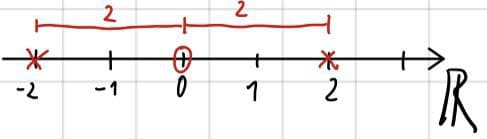
\includegraphics[width=.3\textwidth]{Dateien/05/05Quadrik1.jpg}
\end{center}
\end{Beispiel}
\begin{Beispiel}
{Verschobene Quadrik in 1D (2/7)}
Die Gleichung $\boxed{x^2-2x-8=0}$ können wir durch quadratische Ergänzung in die Form $(x-1)^2=9$ bringen. Die beiden Lösungen können wir uns ebenfalls als 1D-Kugel um den um 1 verschobenen Mittelpunkt vorstellen:
\begin{center}
    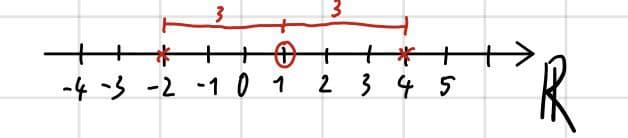
\includegraphics[width=.3\textwidth]{Dateien/05/05Quadrik2.jpg}
\end{center}
\end{Beispiel}

\begin{Beispiel}
{Quadrik in 2D: Kreis (3/7)}
Im Zweidimensionalen ist die einfachste Form einer Quadrik ein Kreis um den Ursprung mit $\boxed{x^2+y^2=16}$.
Wie man sich schnell mit dem Satz des Pythagoras klarmachen kann, sind dies alle Punkte $(x,y)$ mit Abstand $\sqrt{16}=4$ vom Ursprung:
\begin{center}
    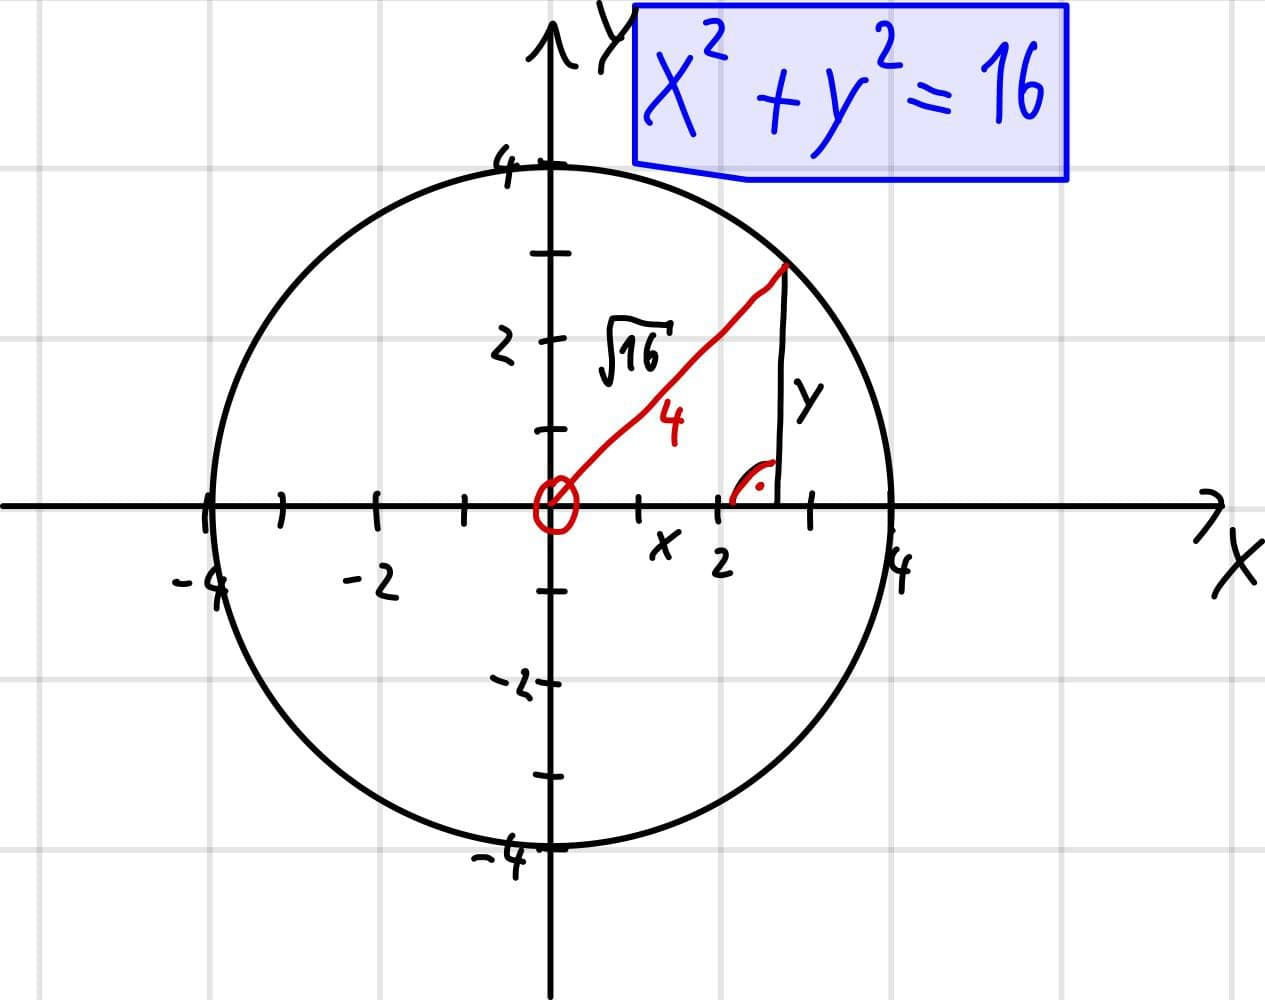
\includegraphics[width=.3\textwidth]{Dateien/05/05Quadrik3.jpg}
\end{center}
Schreiben wir die Bestimmungsgleichung in Matrixform
\begin{equation}
    \vvec^T A \vvec=16\iff \Matrix{x&y}\Matrix{1&0\\0&1}\Matrix{x\\y}=16,
\end{equation}
so sehen wir hier schon, dass diese Matrix eine Signatur von $(2,0,0)$ hat. Dies ist eine Indikation, dass es sich bei der Gleichung um einen Kreis oder eine Ellipse handelt. Die Hauptachsentransformation kann nun auch kompliziertere Gleichungen klassifizieren, wie im übernächsten Beispiel deutlich wird.
\end{Beispiel}

\begin{Beispiel}
{Verschobene Quadrik in 2D: Kreis (4/7)}
Auch diesen Kreis kann man verschieben: $\boxed{x^2+4x+y^2-2x-11=0}$.\\
Mit quadratischer Ergänzung ist dann der Mittelpunkt leicht zu erkennen:\\
$\iff (x+2)^2+(y-1)^2=16$, was dann so aussieht:
\begin{center}
    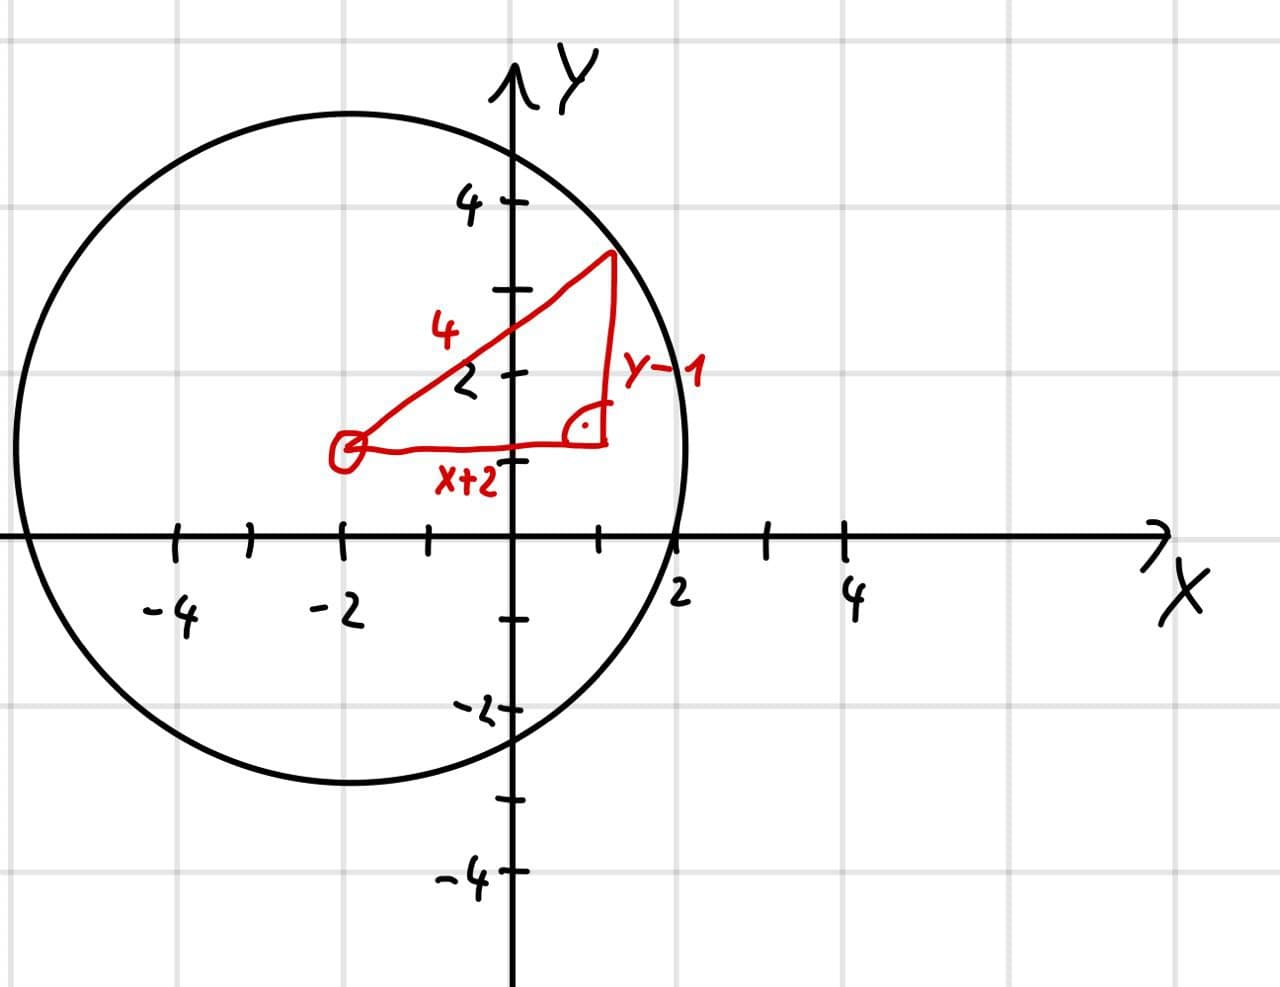
\includegraphics[width=.3\textwidth]{Dateien/05/05Quadrik4.jpg}
\end{center}
\end{Beispiel}

\begin{Beispiel}
{Verschobene Quadrik in 2D: Ellipse (5/7)}
Ähnlich sind Ellipsen zu handhaben.\\
Deren einfachste Form ist $\frac{x^2}{a^2}+\frac{y^2}{b^2}=1$, wobei $a$ und $b$ die \red{Halbachsen} in $x$- und $y$-Richtung sind (auch wieder mit dem Satz des Pythagoras zu sehen). Diese können dann analog zum Kreis verschoben werden.\\
Wir können z. B. $\boxed{\frac{(x-1)^2}{9}+\frac{(y+3)^2}{4}=1}$ (mit dem Mittelpunkt $x=1, y=-3$ und $a=3$ und $b=2$) als Beispiel betrachten:
\begin{center}
    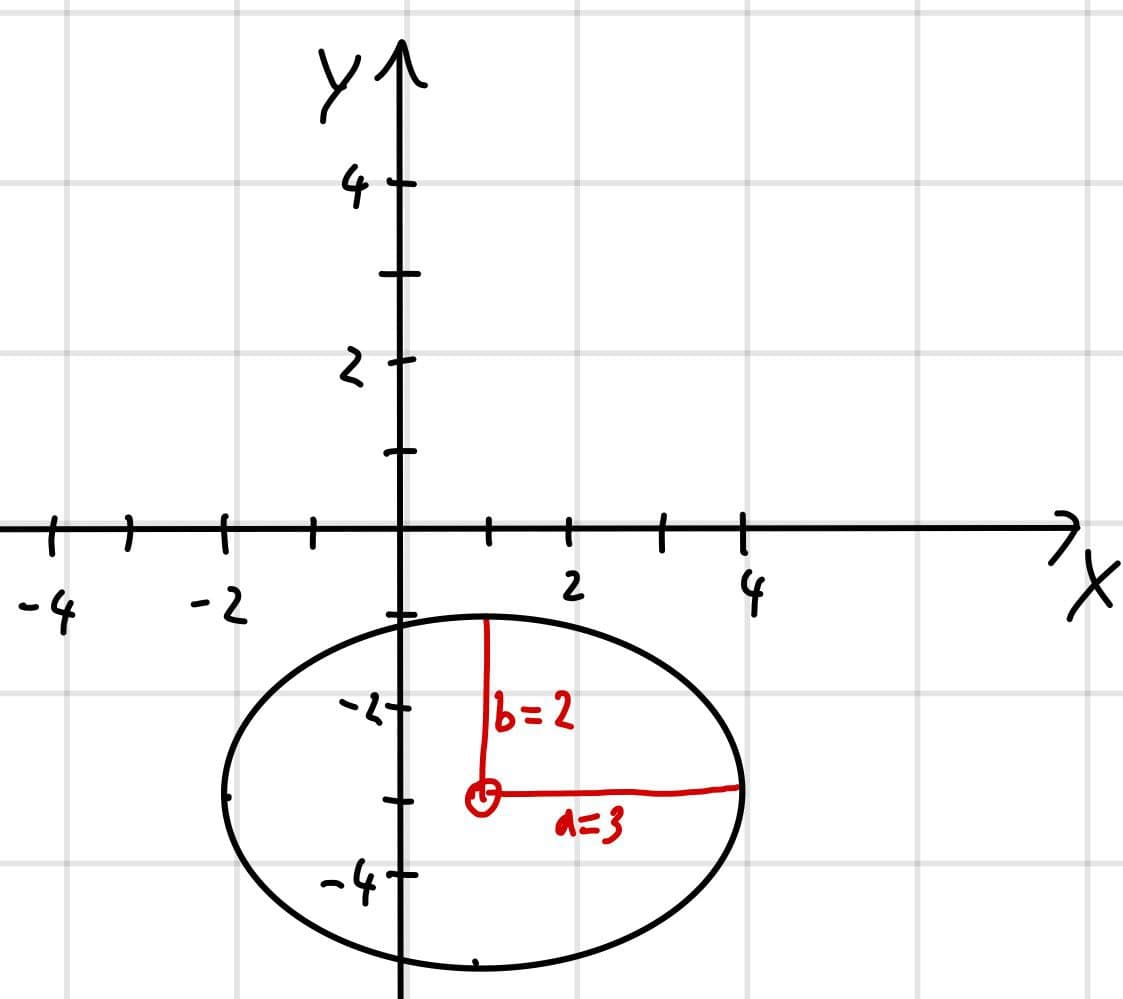
\includegraphics[width=.23\textwidth]{Dateien/05/05Quadrik5.jpg}
\end{center}
\end{Beispiel}
\blue{Wir bekommen bei so etwas allerdings Probleme, sobald Mischterme in unseren Gleichungen auftreten. Diese liefern einen Hinweis darauf, dass die Ellipse gedreht wurde.\\
Um nun die Halbachsen ablesen zu können, müssen wir diese auf die Hauptachse \textit{zurückdrehen}.\\
Hier kommt die Hauptachsentransformation ins Spiel.}
\subsubsection{Drehung einer Quadrik}
\begin{Beispiel}
{Gedrehte Quadrik in 2D: Ellipse und Anwendung der HATrafo (6/7)}
Wir betrachten die Gleichung $\boxed{5x^2-64x+5y^2-32y+6xy+176=0}$ und wollen diese geometrisch interpretieren.\\
Mit $\vvec:=\MatrixInline{x\\y}$ können wir die Gleichung schreiben als
\begin{equation*}
    \Matrix{x & y}\Matrix{5&6/2\\6/2&5}\Matrix{x\\y}+ \Matrix{-64&-32}\Matrix{x\\y}+176=0\iff \vvec^T A \vvec+ \bvec^T\vvec +176 =0,
\end{equation*}
wobei wir $\bvec=-32\MatrixInline{2\\1}$ und $A=\MatrixInline{5&6/2\\6/2&5}$ definieren\footnote{den $xy$-Anteil haben wir hier halbiert, damit die Matrix symmetrisch wird.} bzw. abgelesen haben.\\
Um die Ellipse jetzt \textit{zurückzudrehen}, müssen wir die Eigenwerte $\lambda_i$ und die normierten Eigenvektoren $\wvec_i$ von $A$ finden.
\begin{itemize}
    \item Wir finden 
    \begin{equation*}
        \lambda_1=8\implies \wvec_1=\frac{1}{\sqrt{2}}\Matrix{1\\1},\quad \lambda_2=2\implies \wvec_2=\frac{1}{\sqrt{2}}\Matrix{1\\-1}
    \end{equation*}
    Die diagonalisierte Matrix ist damit
    \begin{equation*}
        D_A=\Matrix{8&0\\0&2},
    \end{equation*}
    was wir testen können, indem wir als $\phi_B$ die Basis der EV bezeichnen:
    \begin{equation*}
        A=\phi_B^{-1} D_A\phi_B=\frac{1}{\sqrt{2}}\Matrix{1&1\\1&-1}\Matrix{8&0\\0&2}\frac{1}{\sqrt{2}}\Matrix{1&1\\1&-1}=\frac{1}{2}\Matrix{10&6\\6&10}=\Matrix{5&3\\3&5}.
    \end{equation*}
    \item Da die Eigenwerte beide positiv sind, ist die Normalform $N_A=\Matrix{1&0\\0&1}$ bzgl. der orthogonalen Basis
\begin{equation*}
    \bvec_1=\frac{\wvec_1}{\sqrt{\Abs{\lambda_1}}\Norm{\wvec_1}}=\frac{1}{\sqrt{8}\sqrt{2}}\Matrix{1\\1}=\frac{1}{4}\Matrix{1\\1},\quad \bvec_2=\frac{1}{2}\Matrix{1\\-1},
\end{equation*}
die Signatur ist also ebenfalls $(2,0,0)$, es handelt sich um eine Ellipse.\footnote{Z. B. beschreiben Gleichungen der Form $(1,1,0)$ Hyperbeln.}
\begin{center}
    \includegraphics[width=.35\textwidth]{Dateien/05/05DrehungHauptachsen.jpg}
\end{center}
    Damit wir diese Drehung auf die Quadrik anwenden wollen, müssen wir tatsächlich die Normierten Versionen $\bvec_1'=\frac{1}{\sqrt{2}}\MatrixInline{1\\1}$ und $\bvec_2'=\frac{1}{\sqrt{2}}\MatrixInline{1\\-1}$ verwenden, welche in Kombination die Drehmatrix\footnote{also eine lineare Abbildung, bei der die Länge der Vektoren erhalten bleibt, oder auch \textit{orthogonaler Endomorphismus}.} $\mathcal{D}=\frac{1}{\sqrt{2}}\MatrixInline{1&1\\1&-1}$ ergeben, denn
    \begin{equation*}
        \BiFo{\mathcal{D}\vvec,\mathcal{D}\vvec}=(\mathcal{D}\vvec)^T(\mathcal{D}\vvec)=\vvec^T\mathcal{D}^T\mathcal{D} \vvec=\vvec^T\mathds{1}_2\vvec=\BiFo{\vvec,\vvec}.
    \end{equation*}
    Wie oben gesehen, gilt $\mathcal{D}^TA\mathcal{D}=\MatrixInline{8&0\\0&2}$.
    \item Um unsere Gleichung nun in anschauliche Form zu bringen, müssen wir zudem den Vektor $\bvec$ drehen.\\
    Dafür substituieren wir $\vvec=\mathcal{D}\wvec=\mathcal{D}\MatrixInline{x'\\y'}$:
    \begin{eqnarray*}
        0&=&\vvec^T A\vvec-32\bvec^T \vvec+176\\
        \iff0&=&(\mathcal{D}w)^TA \mathcal{D}\wvec-32 \bvec^T\mathcal{D}\wvec+176\\
        \iff 0&=&\wvec^T D_A \wvec+\frac{1}{\sqrt{2}} \bvec^T\Matrix{x'+y'\\x'-y'}+176\\
        \overset{\footnote{Nebenrechnung: $\bvec^T \mathcal{D}\wvec=\MatrixInline{2&1}\MatrixInline{x'+y'\\x'-y'}=2x'+2y'+x'-y'=3x'+y'$}}{\iff} 0&=&8x{'}^2+2y{'}^2-\frac{96}{\sqrt{2}}x'-\frac{32}{\sqrt{2}}y'+176\\
        \overset{\footnote{Nebenrechnung: Zweifache quadratische Ergänzung:\\
        $8(x{'}^2-2\frac{96}{2\cdot 8\sqrt{2}}x'+\frac{6^2}{2}-18)=8(x'-6/\sqrt{2})^2-18\cdot 8$ und\\
        $2(y{'}^2-2\frac{32}{2\cdot 2\sqrt{2}}y'+32-32=2(y'-8/\sqrt{2})^2-32\cdot 2$}}{\iff} 0&=&8\BracedIn{x'-\frac{6}{\sqrt{2}}}^2-144+2\BracedIn{y'-\frac{8}{\sqrt{2}}}^2-64+176\\
        \overset{\footnote{Koordinatentransformation: Wir wählen $x''=x'-\frac{6}{\sqrt{2}}$ und $y''=y'-\frac{8}{\sqrt{2}}$}}{\iff} 32&=&8x{''}^2+2y{''}^2\\
        \iff 1&=&\BracedIn{\frac{x''}{2}}^2+\BracedIn{\frac{y''}{4}}^2.
    \end{eqnarray*}
    Endlich haben wir also unsere bekannte Ellipsenform gefunden!\\
    Es handelt sich also um eine Ellipse mit den Halbachsen $a=2$ und $b=4$, die um $\frac{6}{\sqrt{2}}$ und $\frac{8}{\sqrt{2}}$ verschoben und dann gedreht wurde.
    \item Über eine Rücktransformation kommen wir wieder auf die ursprünglichen Koordinaten:
    \begin{itemize}
        \item Translation: $x''=x'-\frac{6}{\sqrt{2}}$ und $y''=y'-\frac{8}{\sqrt{2}}$ ergibt
        \begin{equation*}
            \BracedIn{\frac{x'-6/\sqrt{2}}{2}}^2+\BracedIn{\frac{y'-8/\sqrt{2}}{4}}^2=1.
        \end{equation*}
        \item Drehung: $\MatrixInline{x\\y}=\mathcal{D}\wvec=\frac{1}{\sqrt{2}}\MatrixInline{x'+y'\\x'-y'}$.\\
        Die Umkehrung davon können wir durch ein Gleichungssystem oder durch Invertieren von $\mathcal{D}$ finden (in diesem Fall gilt $\mathcal{D}^{-1}=\mathcal{D}^T$).\\
        Es zeigt sich, dass $ \MatrixInline{x'\\y'}=\frac{1}{\sqrt{2}}\MatrixInline{x+y\\x-y}$. Somit finden wir:
        \begin{equation*}
            \BracedIn{\frac{x+y-6}{2\sqrt{2}}}^2+\BracedIn{\frac{x-y-8}{4\sqrt{2}}}^2=1.
        \end{equation*}
    \end{itemize}
\end{itemize}
\begin{center}
    \includegraphics[width=.95\textwidth]{Dateien/05/05DrehungEllipse.jpg}
\end{center}
\end{Beispiel}

\begin{Beispiel}
    {Quadriken in 3D (für Mutige!) (7/7)}
    Wir betrachten die folgende Gleichung:
    \begin{equation*}
        7x^2-2y^2+7z^2+8xy-10xz+8yz+\sqrt{6}x-\sqrt{6}y+1=0.
    \end{equation*}
    Wer jetzt noch nicht die Flucht ergriffen hat, kann sich überlegen, wie man diese Gleichung in Matrizenschreibweise ausdrücken kann. Tatsächlich ist das nämlich gar nicht so übel wie es aussieht. Wir müssen nur vorher die beiden Terme mit der Wurzel abspalten.\\
    Damit erhalten wir:
    \begin{equation*}
        \Matrix{x&y&z}\Matrix{7&4&-5\\4&-2&4\\-5&4&7}\Matrix{x\\y\\z} + \Matrix{\sqrt{6}&-\sqrt{6}&0}\Matrix{x\\y\\z} + 1 = 0.
    \end{equation*}
    Das Ziel dieser Rechnung ist es, herauszufinden, welche geometrische Form diese Gleichung beschreibt.\\
    Dazu wenden wir, wie in den vorherigen Beispielen auch, die Hauptachsentransformation auf die $3\times3$-Matrix an. Da ihr ja mittlerweile Experten seit, rechnen wir die folgenden Schritte nicht ganz so detailliert durch, die Rechnung sollte aber trotzdem gut nachvollziehbar sein.\\
    Fangen wir mit dem charakteristischen Polynom an:
    \begin{equation*}
        0=\det\Matrix{7-\lambda&4&-5\\4&-2-\lambda&4\\-5&4&7-\lambda}=(-6-\lambda)(6-\lambda)(12-\lambda).
    \end{equation*}
    Hier können wir die Eigenwerte $\lambda_1=12$, $\lambda_2=6$ und $\lambda_3=-6$ bequem ablesen. Aus der Diagonalmatrix bekommen wir die Signatur:
    \begin{equation*}
        \Matrix{12&0&0\\0&6&0\\0&0&-6} \qquad \Rightarrow \qquad r_+=2 \quad r_-=1 \quad r_0=0.
    \end{equation*}
    Außerdem können wir die Eigenvektoren bestimmen:
    \begin{align*}
        \lambda_1&=12: \qquad \Matrix{-5&4&-5\\4&-14&4\\-5&4&-5}\Matrix{x\\y\\z}=\Matrix{0\\0\\0} \qquad \Rightarrow \qquad \vvec_1=t\Matrix{1\\0\\-1} \\
        \lambda_2&=6: \qquad \Matrix{1&4&-5\\4&-8&4\\-5&4&1}\Matrix{x\\y\\z}=\Matrix{0\\0\\0} \qquad \Rightarrow \qquad \vvec_2=t\Matrix{1\\1\\1} \\
        \lambda_3&=-6: \qquad \Matrix{13&4&-5\\4&4&4\\-5&4&13}\Matrix{x\\y\\z}=\Matrix{0\\0\\0} \qquad \Rightarrow \qquad \vvec_3=t\Matrix{1\\-2\\1}
    \end{align*}
    und damit die Basis der Normalform anhand der bereits bekannten Formel:
    \begin{align*}
        \wvec_1'&=\frac{\vvec_1}{\lambda_1\Vert \vvec_1\Vert}=\frac{1}{2\sqrt{6}}\Matrix{1\\0\\-1} \\
        \wvec_2'&=\frac{\vvec_2}{\lambda_2\Vert \vvec_2\Vert}=\frac{1}{3\sqrt{2}}\Matrix{1\\1\\1} \\
        \wvec_3'&=\frac{\vvec_3}{\lambda_3\Vert \vvec_3\Vert}=\frac{1}{6}\Matrix{1\\-2\\1}. 
    \end{align*}
    Wenn ihr möchtet, könnt ihr überprüfen, ob diese Vektoren tatsächlich zum richtigen Ergebnis führen.\\
    Sei dazu $F:\mathbb{R}^3 \Rightarrow \mathbb{R}, \, F(\vvec_1,\vvec_2):=\vvec_1^T A \vvec_2$ mit einer $3\times3$-Matrix $A$, dann erhalten wir:
    \begin{equation*}
        A:=\Matrix{7&4&-5\\4&-2&4\\-5&4&7} \qquad \Rightarrow \qquad (F(\wvec_i',\wvec_j'))_{ij}=\Matrix{1&0&0\\0&1&0\\0&0&-1}
    \end{equation*}
    Nun folgt die eigentliche Anwendung auf die Quadrik. Diese dürfen wir nur drehen und verschieben, da ja die Form beibehalten werden soll (um später identifizieren zu können, um welchen Kegelschnitt es sich handelt). \\
    Der erste Schritt dafür ist, die Vektoren $\wvec_1'$, $\wvec_2'$ und $\wvec_3'$ zu orthonormalisieren:
    \begin{align*}
        \wvec_1&=\frac{\wvec_1'}{\Vert \wvec_1' \Vert} = \frac{1}{\sqrt{2}}\Matrix{1\\0\\-1} \\
        \wvec_2&=\frac{\wvec_2'}{\Vert \wvec_2' \Vert} = \frac{1}{\sqrt{3}}\Matrix{1\\1\\1} \\
        \wvec_3&=\frac{\wvec_3'}{\Vert \wvec_3' \Vert} = \frac{1}{\sqrt{6}}\Matrix{1\\-2\\1}.
    \end{align*}
    Wir können uns auch hier wieder überzeugen, dass nun:
    \begin{equation*}
        (F(\wvec_i,\wvec_j))_{ij}=\Matrix{12&0&0\\0&6&0\\0&0&-6}.
    \end{equation*}
    Nun beginnt die eigentliche Zauberei der Hauptachsentransformation.\\
    Wenn ihr bis hierhin gut aufgepasst habt, wisst ihr, dass man die Matrix $A$ in ihre Diagonalform transformieren kann, wenn man die orthonormierten Basisvektoren als Spalten in eine Matrix $B$ schreibt:
    \begin{equation*}
        B:=\Matrix{\frac{1}{\sqrt{2}}&\frac{1}{\sqrt{3}}&\frac{1}{\sqrt{6}}\\0&\frac{1}{\sqrt{3}}&-\frac{2}{\sqrt{6}}\\-\frac{1}{\sqrt{2}}&\frac{1}{\sqrt{3}}&\frac{1}{\sqrt{6}}}.
    \end{equation*}
    Diese Matrix ist eine Drehmatrix! Dies kann man sich durch
    \begin{equation*}
        \langle Bv, Bw \rangle = \sum_{i,j=1}^{3}x_ix_j\langle \wvec_i, \wvec_j \rangle = \sum_{i,j=1}^{3} x_i y_j \delta_{ij} = \sum_{i=1}^{3} x_i y_i = \langle x,y \rangle
    \end{equation*}
    deutlich machen, da die Vektoren $\wvec_i$ orthogonal aufeinander stehen. \\
    Sei nun $\vvec=(x,y,z)^T$. In unsere ursprüngliche Gleichung setzen wir nun $\vvec=B\uvec$ mit einem beliebigen Vektor $\uvec$:
    \begin{align*}
        \uvec^T B^T \Matrix{7&4&-5\\4&-2&4\\-5&4&7}B\uvec + \Matrix{\sqrt{6}&-\sqrt{6} 0}B\uvec + 1 = 0 \\
        \Rightarrow \uvec^T\Matrix{12&0&0\\0&6&0\\0&0&-6}\uvec + \Matrix{\sqrt{3}&0&3}\uvec + 1 = 0
    \end{align*}
    Damit sind die Mischterme (also $axy$, $byz$ usw.) in der ursprünglichen Gleichung erfolgreich eliminiert (nice!).\\
    Alles Weitere ist nun geschicktes Umformen.\\
    Wir definieren dazu unser Koordinatensystem um und setzen $\uvec=\Matrix{x&y&z}^T$:
    \begin{align*}
        &12x^2+6y^2-6z^2+\sqrt{3}x+3z+1=0 \\
        \Leftrightarrow &12(x+\frac{\sqrt{3}}{24})^2-\frac{3}{48}+6y^2-6(z-\frac{1}{4})^2+\frac{3}{8} + 1 = 0 \\
        \Leftrightarrow &12(x+\frac{\sqrt{3}}{24})^2 + 6y^2 - 6(z-\frac{1}{4})^2 = -\frac{21}{16}.
    \end{align*}
    Nun führen wir eine Translation durch, indem wir $x$, $y$ und $z$ erneut umdefinieren:
    \begin{equation*}
        x \longrightarrow x-\frac{\sqrt{3}}{24} \qquad y \longrightarrow y \qquad z \longrightarrow z+\frac{1}{4}
    \end{equation*}
    Dadurch erhalten wir
    \begin{align*}
        12x^2+6y^2-6z^2=-\frac{21}{16} \\
        \Leftrightarrow -\frac{x^2}{\alpha_1^2}-\frac{y^2}{\alpha_2^2}+\frac{z^2}{\alpha_3^2}=1,
    \end{align*}
    wobei wir im letzten Schritt die folgenden Abkürzungen verwendet haben:
    \begin{equation*}
        \alpha_1 = \sqrt{\frac{7}{64}} \qquad \alpha_2 = \sqrt{\frac{7}{32}} \qquad \alpha_3 = \sqrt{\frac{7}{32}}
    \end{equation*}
    Diese nun sehr kompakte Gleichung beschreibt dieselbe Form wie vorher, wir haben sie nur etwas gedreht und verschoben\footnote{bzw. haben wir das \textit{Koordinatensystem} gedreht und verschoben.}. Der Vorteil an dieser kompakten Form ist nun, dass wir ganz leicht die Art des Kegelschnittes ablesen können (etwas Übung vorausgesetzt natürlich).\\
    In diesem Fall handelt es sich um ein \red{zweischaliges Hyperboloid}. \\
    Die abschließende Abbildung hilft hoffentlich dabei, sich den Vorgang auch in 3D bildlich vorstellen zu können.
    \begin{center}
        \includegraphics[width=.95\textwidth]{Dateien/05/05Quadrik6.JPG}
    \end{center}
\end{Beispiel}

\subsection{Vollständige metrische Räume}
\blue{Lasst uns nun zum nächsten Thema kommen: Vollständige metrische Räume und der banachsche Fixpunktsatz. Dazu müssen wir uns zunächst durch ein paar Definitionen und Wiederholungen kämpfen.}
\begin{Wiederholung}
{Metrik}
Eine Abstandsfunktion oder \red{Metrik $d$} ordnet zwei Elementen einer Menge $X$ eine positive reelle Zahl zu und hat die folgenden Eigenschaften:\\
$d:X\times X\to [0,\infty)$
\begin{eqnarray*}
\red{M1}: & d(x,y)\geq 0\text{ und } d(x,y)=0\Leftrightarrow x= y &\red{'positiv definit'}\\
\red{M2}: & d(x,y)=d(y, x) &\red{'symmetrisch'}\\
\red{M3}: & d(x,y)\leq d(x, z)+d(y,z) & \red{'Dreiecksungleichung'}.
\end{eqnarray*}
\end{Wiederholung}
\begin{Def}
{Metrischer Raum}
Wir nennen eine Menge $X$ zusammen mit einer Metrik einen \red{metrischen Raum}.
\end{Def}
\begin{Beispiel}
{Die reellen Zahlen als metrischer Raum}
Mit dem der Differenz des Betrages als Abstandsfunktion\\ ($d:\mathbb{R}\times\mathbb{R}\to[0,\infty)\,d(x,y):=\Abs{x-y}$) sind die reellen Zahlen ein metrischer Raum, wie wir in Mathe 1 gesehen hatten.
\end{Beispiel}

\begin{Def}
{Norm}
Falls wir Vektorräume $V$ über $\mathbb{K}$ betrachten, können wir dort noch den Begriff der \red{Norm} spezifizieren, der jedem Vektor $\vvec\in V$ eine Länge zuordnet:
\begin{equation}
    \Norm{\cdot}:V\to[0,\infty),\quad \vvec\mapsto\Norm{\vvec}.
\end{equation}
Zudem müssen die drei \textit{Normaxiome} N1, N2 und N3 erfüllt sein:
\begin{itemize}
    \item N1: \red{Positive Definitheit}: $\Norm{\vvec}=0\iff \vvec=0$ für $\vvec\in V$.
    \item N2: \red{Homogenität (Skalierung)}: $\Norm{\lambda \vvec}=\Abs{\lambda}\Norm{\vvec}$ für alle $\vvec\in V,\lambda \in\mathbb{K}$.
    \item N3: \red{Dreiecksungleichung}: $\Norm{\vvec+\wvec}\leq\Norm{\vvec}+\Norm{\wvec}$ für alle $\vvec,\wvec\in V$ \blue{(i. d. R. am schwierigsten zu zeigen).}
\end{itemize}
\end{Def}
\red{Achtung: Bisher hatten wir nur Normen kennengelernt, die durch ein Skalarprodukt \textit{induziert} wurden ($\Norm{\vvec}=\sqrt{\BiFo{\vvec,\vvec}}$). Dies muss aber nicht unbedingt der Fall sein!}
\begin{Beispiel}
{Die Maximumsnorm auf dem $\mathbb{R}^n$}
\Zz{Durch $\Norm{\xvec}_\tx{max}:=\max(\Abs{x_1},\Abs{x_2},\ldots,\Abs{x_n})$ ist auf $V=\mathbb{R}^n$ eine Norm definiert.}
Anwendungsbeispiel: Sei $\vvec=\MatrixInline{1\\-8\\2}\in\mathbb{R}^3\implies\Norm{\vvec}_\tx{max}=\max(1,8,2)=8$.\\
\Zb{Wir zeigen, dass $\Norm{\cdot}_{\max}$ die Normaxiome erfüllt.
\begin{itemize}
    \item N1)
    \begin{itemize}
        \item \grqq$\implies$\grqq: Für $\Norm{\xvec}_{\max}=0$ muss $\xvec$ der Nullvektor sein, denn wäre O.B.D.A.\footnote{Ohne Beschränkung der Allgemeinheit} der erste Eintrag ungleich 0, so wäre $\Norm{\xvec}_{\max}=\max(\Abs{x_1},0,\ldots,0)=\Abs{x_1}\neq0$, was im Widerspruch zur Annahme steht.
        \item \grqq$\impliedby$\grqq: Ist $\xvec=0$, so ist $\Norm{\xvec}_{\max}=\max(0,\ldots,0)=0.\,\checkmark$
    \end{itemize}
    \item N2) $\forall\lambda\in\mathbb{R},\,\,\xvec\in\mathbb{R}^n$ gilt:
    \begin{align*}
        \Norm{\lambda \xvec}_\tx{max}&=\max(\Abs{\lambda x_1},\Abs{\lambda x_2},\ldots,\Abs{\lambda x_n})\\
        &=\max(\Abs{\lambda}\Abs{ x_1},\Abs{\lambda}\Abs{ x_2},\ldots,\Abs{\lambda}\Abs{ x_n})\\
        &=\Abs{\lambda}\max(\Abs{x_1},\ldots,\Abs{x_n})=\Abs{\lambda}\Norm{\xvec}_\tx{max}.\,\checkmark
    \end{align*}
    \item N3) Wir müssen zeigen: $\Norm{\xvec+\yvec}_\tx{max}\leq\Norm{\xvec}_\tx{max}+\Norm{\yvec}_\tx{max}\,\forall \xvec,\yvec\in\mathbb{R}^n$:
    \begin{eqnarray*}
        \Norm{\xvec+\yvec}_\tx{max}&=&\max(\Abs{x_1+y_1},\ldots,\Abs{x_n+y_n})\\
        &\overset{\footnote{Wir nutzen die Dreiecksungleichung für den Betrag für jede Komponente.}}{\leq}&\max(\Abs{x_1}+\Abs{y_1},\ldots,\Abs{x_n}+\Abs{y_n})\\
        &\overset{\footnote{Wir nutzen $\max(\Abs{a}+\Abs{b})=\Abs{a}+\Abs{b}\leq\max(\Abs{a})+\max(\Abs{b})$}}{\leq}&\max(\Abs{x_1},\ldots,\Abs{x_n})+\max(\Abs{y_1},\ldots,\Abs{y_n})\\
        &=&\Norm{\xvec}_\tx{max}+\Norm{\yvec}_\tx{max}.\,\checkmark
    \end{eqnarray*}
\end{itemize}
}
\end{Beispiel}
\begin{Satz}
{Anmerkung}{Vom Skalarprodukt induzierte Norm}
In euklidischen/hermiteschen Vektorräumen $(V,\BiFo{\cdot,\cdot})$ ist stets die vom Skalarprodukt induzierte Norm durch $\Norm{\vvec}=\sqrt{\BiFo{\vvec,\vvec}}$ auf $V$ definiert.\\
Diese erfüllt die Normaxiome, denn:
\begin{itemize}
    \item N1) folgt aus der positiven Definitheit des Skalarproduktes.
    \item N2) Es ist $\Norm{\lambda \vvec}^2=\BiFo{\lambda \vvec,\lambda \vvec}\overset{\footnote{$(\mathbb{C})$-Linearität}}{=}\Abs{\lambda}^2\BiFo{\vvec,\vvec}=\Abs{\lambda}^2\Norm{\vvec}^2$.
    \item N3) Es ist
    \begin{eqnarray*}
    \Norm{\vvec+\wvec}^2&=&\BiFo{\vvec+\wvec,\vvec+\wvec}\overset{\footnote{Bilinearität}}{=}\BiFo{\vvec,\vvec}+\BiFo{\vvec,\wvec}+\BiFo{\wvec,\vvec}+\BiFo{\wvec,\wvec}\\
    &\overset{\footnote{Hermitizität, $\frac{1}{2}(\BiFo{\vvec,\wvec}+\overline{\BiFo{\vvec,\wvec}})=\Re(\BiFo{\vvec,\wvec})$}}{=}&\Norm{\vvec}^2+\Norm{\wvec}^2+2\Re(\BiFo{\vvec,\wvec})\overset{\footnote{Gleichheit gilt, wenn $\Re(\BiFo{\vvec,\wvec})=\Abs{\BiFo{\vvec,\wvec}}$}}{=}\Norm{\vvec}^2+\Norm{\wvec}^2+2\Abs{\BiFo{\vvec,\wvec}}\\
    &\overset{\footnote{Cauchy-Schwarzsche Ungleichung}}{\leq}&\Abs{\vvec}^2+\Abs{\wvec}^2+2\Norm{\vvec}\Norm{\wvec}\overset{\footnote{Binomische Formeln}}{=}(\Norm{\vvec}+\Norm{\wvec})^2.
    \end{eqnarray*}
\end{itemize}
\end{Satz}
\blue{Mithilfe der folgenden Gleichung können wir überprüfen, ob eine vorgegebene Norm durch ein Skalarprodukt induziert wurde:}
\begin{Satz}
{Satz}{Parallelogrammgleichung}
Genau dann wenn eine Norm $\Norm{\cdot}$ auf einem Vektorraum $V$ über $\mathbb{R}$ durch ein Skalarprodukt induziert wird, gilt die \red{Parallelogrammgleichung}
\begin{equation*}
    \Norm{\vvec+\wvec}^2+\Norm{\vvec-\wvec}^2=2\Norm{\vvec}^2+2\Norm{\wvec}^2\quad \forall \vvec,\wvec\in V.
\end{equation*}
\begin{center}
    \includegraphics[width=.5\textwidth]{Dateien/05/05Parallelogramm.jpg}
\end{center}
\end{Satz}
\begin{Beispiel}
{Beweis in die eine Richtung}
Wir zeigen kurz, dass dies mit einer vom Skalarprodukt induzierten Norm klappt:
\begin{align*}
    \Norm{\vvec+\wvec}^2+\Norm{\vvec-\wvec}^2&=\BiFo{\vvec+\wvec,\vvec+\wvec}+\BiFo{\vvec-\wvec,\vvec-\wvec}\\
    &=\BiFo{\vvec,\vvec}+2\Re(\BiFo{\vvec,\wvec})+\BiFo{\wvec,\wvec}+\BiFo{\vvec,\vvec}-2\Re(\BiFo{\vvec,\wvec})+\BiFo{\wvec,\wvec}\\
    &=2\BiFo{\vvec,\vvec}+2\BiFo{\wvec,\wvec}.
\end{align*}
Die andere Richtung ist aufwändiger, siehe \Skript{}.
\end{Beispiel}

\begin{Satz}
{Anmerkung}{Verknüpfung der Norm zur Metrik}
Jede Norm definiert durch $d:V\times V\to [0,\infty),\,d(\xvec,\yvec)=\Norm{\xvec-\yvec}$ auch eine Metrik auf $V$, denn die Metrikaxiome M1), M2) und M3) folgen aus den Eigenschaften der Norm:
\begin{itemize}
    \item M2): $d(\xvec,\yvec)=\Norm{\xvec-\yvec}=\Norm{(-1)(\yvec-\xvec)}\overset{\tx{N2)}}{=}\Abs{-1}\Norm{\yvec-\xvec}=\Norm{\yvec-\xvec}=d(\yvec,\xvec)$.
    \item M3): $d(\xvec,\zvec)=\Norm{\xvec-\zvec}=\Norm{\xvec+\yvec-\yvec-\zvec}\overset{\tx{N3)}}{\leq}\Norm{\xvec-\yvec}+\Norm{\yvec-\zvec}=d(\xvec,\yvec)+d(\yvec,\zvec)$.
\end{itemize}
\end{Satz}
\subsubsection{Offene Kugel für verschiedene Metriken}
Wir machen nun einen Vorgriff auf eine kommende Definition, um Unterschiede zwischen verschiedenen Metriken zu verdeutlichen:
\begin{Def}
{Offene Kugel}
Die Teilmenge $\boxed{B_r(\xvec):=\Menge{\yvec\in X}{d(\xvec,\yvec)<r}\subseteq X}$ eines metrischen Raumes $(X,d)$ mit Abstandsfunktion $d$ heißt \red{offene Kugel} mit Mittelpunkt $\xvec$ und Radius $r$.
\end{Def}
\blue{Diese Definition können wir uns z. B. im $\mathbb{R}^3$ mit der euklidischen Metrik tatsächlich als herkömmliche Kugel vorstellen.\\
Aber Achtung: Je nach Metrik kann eine solche 'offene Kugel' anders aussehen!}\\
Für die folgenden Beispiele betrachten wir $B_1(0)$ im $\mathbb{R}^2$ (also eine Kugel um 0 mit Radius 1).
\begin{Beispiel}{Euklidische Metrik (1/3)}
Mit der euklidischen Metrik $d_2(\xvec,\yvec)=\sqrt{\sum_{i=1}^2\Abs{x_i-y_i}^2}$ ist die offene Kugel einfach ein Kreis.\\ $B_1(0)$ sieht also so aus:
\begin{center}
    \includegraphics[width=.35\textwidth]{Dateien/05/05Metrik1.jpg}
\end{center}
\end{Beispiel}
\begin{Beispiel}
{Summenmetrik (2/3)}
Mit der Summenmetrik $d_1(\xvec,\yvec):=\sum_{i=1}^2\Abs{x_i-y_i}$ ist die offene Kugel hingegen ein gedrehtes Quadrat, dessen Kantenlänge in diesem Fall $\sqrt{2}$ ist.\\ Hier sieht $B_1(0)$ so aus:
\begin{center}
    \includegraphics[width=.35\textwidth]{Dateien/05/05Metrik2.jpg}
\end{center}
\end{Beispiel}
\begin{Beispiel}
{Maximumsmetrik (3/3)}
Mit der Maximumsmetrik $d_\tx{max}(\xvec,\yvec):=\max(\Abs{x_1-y_1},\Abs{x_2-y_2})$ ist die offene Kugel ein Quadrat mit Kantenlänge 2.\\ Hier sieht $B_1(0)$ so aus:
\begin{center}
    \includegraphics[width=.35\textwidth]{Dateien/05/05Metrik3.jpg}
\end{center}
\end{Beispiel}

\begin{Def}
{Äquivalente Normen}
Wir nennen zwei Normen $\Norm{\cdot}_1$ und $\Norm{\cdot}_2$ auf einem Vektorraum \red{äquivalent}, falls es Schranken $c,C\in\mathbb{R}$ gibt, sodass
\begin{equation}
    c\Norm{\vvec}_1\leq\Norm{\vvec}_2\leq C\Norm{\vvec}_1\quad \forall v\in V.
\end{equation}
\end{Def}
\blue{Wir müssen mit der einen Norm also quasi die andere einschränken können, falls sie äquivalent sind.}
\begin{Beispiel}
{Beweis: Die Äquivalenz zwischen Normen ist eine Äquivalenzrelation}
Wir beweisen die obige Aussage.\\
\Zb{Die Normäquivalenz definiert eine Äquivalenzrelation, denn:
\begin{itemize}
    \item Sie ist reflexiv:\\
    Eine beliebige Norm ist mit den Konstanten $c=C=1$ stets zu sich selbst äquivalent.
    \item Sie ist symmetrisch:\\
    Sei $\Norm{\cdot}_1$ zu $\Norm{\cdot}_2$ äquivalent, es gebe also $c,C$ sodass $c\Norm{\vvec}_1\leq\Norm{\vvec}_2\leq C\Norm{\vvec}_1$.\\
    Dann ist aber $\frac{1}{C}\Norm{\vvec}_2\leq\Norm{\vvec}_1\leq\frac{1}{c}\Norm{\vvec}_2$, $\Norm{\cdot}_2$ ist also äquivalent zu $\Norm{\cdot}_1$.
    \item Sie ist transitiv:\\
    Seien $\Norm{\cdot}_1\sim \Norm{\cdot}_2$ und $\Norm{\cdot}_1\sim\Norm{\cdot}_3$, dann ist
    \begin{align*}
        &c\Norm{\vvec}_1\leq\Norm{\vvec}_2\leq C\Norm{\vvec}_1\,\land\, c'\Norm{\vvec}_1\leq\Norm{\vvec}_3\leq C'\Norm{\vvec}_1\\
        \implies & c\Norm{\vvec}_1\leq\frac{c}{c'}\Norm{\vvec}_3\leq\Norm{\vvec}_2\leq\frac{C}{C'}\Norm{\vvec}_3\leq C\Norm{\vvec}_1,
    \end{align*}
    also ist $\Norm{\cdot}_1\sim\Norm{\cdot}_2$.
\end{itemize}}
\end{Beispiel}
\begin{Beispiel}
{Die Maximumsnorm und die Betragssummennorm sind äquivalent}
\Zz{Die Maximumsnorm $\Norm{\xvec}_\tx{max}=\max(\Abs{x_1},\ldots,\Abs{x_n})$ und die Betragssummennorm $\Norm{\xvec}_1=\sum_{i=1}^n\Abs{x_i}$ auf dem $\mathbb{R}^n$ sind äquivalent.}
\Zb{Es gilt:
\begin{equation*}
    \Abs{x_i}\leq\max(\Abs{x_1},\ldots,\Abs{x_n})\,\forall i\overset{\footnote{Wenn wir das für die Summe über alle $i$ machen, finden wir $\sum_{i=1}^n\Abs{x_i}\leq n\max(\Abs{x_1},\ldots,\Abs{x_n})$}}{\implies} \Norm{\xvec}_1\leq n\Norm{\xvec}_\tx{max}.
\end{equation*}}\\
Außerdem gilt
\begin{equation*}
    \Norm{\xvec}_\tx{max}=\max(\Abs{x_1},\ldots,\Abs{x_n})\leq\sum_{i=1}^n\Abs{x_i}=\Norm{\xvec}_1.
\end{equation*}
Mit $c:=1$ und $C:=n$ gilt also $c\Norm{\xvec}_\tx{max}\leq\Norm{\xvec}_1\leq\Norm{\xvec}_\tx{max}$, d. h. $\Norm{\cdot}_1\sim\Norm{\cdot}_\tx{max}$.
\end{Beispiel}
Dass diese beiden Normen auf dem endlichdimensionalen $\mathbb{R}^n$ äquivalent sind, ist kein Wunder, denn:
\begin{Satz}
{Satz}{Äquivalenz von Normen auf endlichdimensionalen Vektorräumen}
Auf endlichdimensionalen Vektorräumen sind zwei beliebige Normen immer äquivalent.
\end{Satz}

\subsection{Kontrahierende Abbildungen und der Banachsche Fixpunktsatz}
\begin{Def}
{Kontrahierende Abbildung}
Wir nennen eine Abbildung $F:X\to X$ auf einem metrischen Raum $(X,d)$ \red{kontrahierend}, wenn $\forall x,y\in X$ gilt:
\begin{equation*}
    d(F(x),F(y))\leq \theta d(x,y)\quad\tx{mit }0\leq\theta <1.
\end{equation*}
\end{Def}
\blue{Das Kriterium können wir (für $d(x,y)\neq0$) auch umschreiben zu
\begin{equation*}
    \frac{d(F(x),F(y))}{d(x,y)}<1,
\end{equation*}
die Funktionswerte liegen also immer näher zusammen als deren Urbilder.}
\begin{Beispiel}
{Kontrahierende Gerade (1/2)}
Die Gerade $g:\mathbb{R}\to\mathbb{R},\,g(x)=2-0.5x$ (wobei $d:\mathbb{R}\times\mathbb{R}\to\mathbb{R}$ die Betragsmetrik sei) ist kontrahierend, denn
\begin{equation*}
    d(g(x),g(y))=\Abs{2-0.5x-(2-0.5y)}=\Abs{-0.5}\Abs{x-y}=0.5\Abs{x-y}=\theta d(x,y).
\end{equation*}
\end{Beispiel}

\begin{Wiederholung}{Mittelwertsatz}
Ist $f:[a,b]\to\mathbb{R}$ stetig und differenzierbar auf $(a,b)$, so existiert ein\\
$\xi\in(a,b)$, sodass $f'(\xi)=\frac{f(b)-f(a)}{b-a}$.
\end{Wiederholung}
\begin{Beispiel}
{Verknüpfung mit dem Mittelwertsatz (1/2)}
Für Funktionen $f:\mathbb{R}\to\mathbb{R}$ mit der Betragsmetrik können wir $\theta$ explizit berechnen:\\
Für gegebene $x,y\in\mathbb{R}$ wissen wir aufgrund des Mittelwertsatzes, dass $\xi\in[x,y]$ existiert, sodass
\begin{equation*}
    \theta=\Abs{f'(\xi)}=\frac{\Abs{f(x)-f(y)}}{\Abs{x-y}}.
\end{equation*}
Nach einer Abschätzung für ganze Intervalle können wir das auf den gesamten Definitionsbereich verallgemeinern.\\
Als Beispiel betrachten wir $F:[1,\infty)\to\mathbb{R},\,x\mapsto \frac{1}{2}x+\frac{1}{x}$.\\
Dann ist $\frac{\Abs{F(x)-F(y)}}{\Abs{x-y}}=\Abs{F'(\xi)}=\Abs{\frac{1}{2}-\frac{1}{\xi^2}}\overset{\footnote{weil $\xi\in[1,\infty)$ ist $\Abs{1/\xi^2}\leq 1$}}{\leq}\frac{1}{2}=:\theta\,\forall x,y\in [1,\infty)$. $F$ ist somit eine kontrahierende Abbildung. 
\end{Beispiel}
Diesen Begriff benötigen wir für den folgenden, erstaunlichen Satz:
\begin{Satz}
{Satz}{Banachscher Fixpunktsatz}
Für jede kontrahierende Abbildung in einem \underline{vollständigen}\footnote{Wdh.: In einem vollständigen Raum konvergiert jede Cauchy-Folge gegen ein Element aus diesem Raum.} metrischen Raum $(X,d)$ existiert ein \underline{eindeutiger} \red{Fixpunkt} $\Tilde{x}\in X$, für den gilt, dass $\boxed{F(\Tilde{x})=\Tilde{x}}$.\\
Zudem konvergiert die Folge $\boxed{x_{k+1}=F(x_k)}$ für alle Anfangswerte $x_0\in X$ gegen den Fixpunkt, $\lim_{n\to\infty}x_n=\Tilde{x}$.
\end{Satz}
\blue{\textbf{Motivation/Anwendung}:\\
Wir werden sehen, dass die Eindeutigkeit dieses Fixpunkts wahnsinnig nützlich werden kann, wenn wir uns gegen Ende des Semesters Differentialgleichungen (DG) anschauen. Dort wird eine der wichtigsten Aussagen sein, dass eine DG der Form $x'=F(x,t)$ mit $x(t_0)=x_0$ \underline{genau eine} Lösung hat, wenn $F$ bestimmte Bedingungen erfüllt.\\
Für den Beweis wird dort der Raum der stetigen Funktionen mit einer Norm verwendet, auf dem ein Integraloperator\footnote{der dann auch noch genauer definiert wird und im Prinzip $F(x,t)$ über $t$ integriert.} stetige Funktionen auf stetige Funktionen abbildet. Diese Abbildung ist kontrahierend und besitzt demnach einen Fixpunkt, der \underline{eindeutige} Lösung. Das Iterationsverfahren aus dem Fixpunktsatz kann dann mit diesem Integraloperator auch zum Finden der Lösung der Differentialgleichung verwendet werden.}
\begin{Beispiel}
{Umgebungskarte (1/3)}
Wenn man eine verkleinerte Karte der Umgebung betrachtet, so existiert genau ein Punkt auf der Karte, der dem Ort entspricht, wo die Karte sich befindet.
\end{Beispiel}

\begin{Beispiel}
{Fixpunkt der Geradenabbildung (2/3)}
Wir hatten gesehen, dass $g:\mathbb{R}\to\mathbb{R},\,g(x)=2-0.5x$ kontrahierend mit $\theta=0.5$ ist.\\
Um den Fixpunkt zu finden, lösen wir die Gleichung
\begin{align*}
    \Tilde{x}=2-0.5\Tilde{x}\iff \frac{3}{2}\Tilde{x}=2\iff \Tilde{x}=\frac{4}{3}.
\end{align*}
Alternativ könnt ihr euch auch daran versuchen, eine explizite Vorschrift für die Folge $x_{k+1}=2-0.5x_k$ zu finden, diese zu beweisen und abschließend noch zu zeigen, dass diese gegen $\frac{4}{3}$ konvergiert. Schreibt uns gern, vielleicht bauen wir das in zukünftige Versionen ein, Stand jetzt hatten wir keine Zeit,\footnote{wobei ihr euch wahrscheinlich fragen werdet, warum gerade \textit{das} nun den Rahmen sprengt :D} uns damit zu befassen.
\end{Beispiel}

\begin{Beispiel}
{Fixpunkt einer weiteren Funktion (3/3)}
Wir hatten oben gesehen, dass $F:[0,\infty)\to[0,\infty),\,x\mapsto \frac{1}{2}x+\frac{1}{x}$ eine kontrahierende Abbildung ist. Der Fixpunkt ist dann gegeben durch
\begin{equation*}
    \Tilde{x}=\frac{\Tilde{x}}{2}+\frac{1}{\Tilde{x}}\iff \frac{1}{2}\Tilde{x}^2=1\overset{\footnote{$-\sqrt{2}$ ist nicht Teil des Definitionsbereiches.}}{\implies} \Tilde{x}=\sqrt{2}.
\end{equation*}
Die Folge $x_{n+1}=F(x_n)=\frac{1}{2}\BracedIn{x_n+\frac{2}{x_n}}$ war in MfP1 genau jene Folge, die ihr genutzt hattet, um zu zeigen, dass die rationalen Zahlen nicht vollständig sind!
\end{Beispiel}

\Tipps{7}{
\begin{enumerate}
    \item Die Signaturbestimmung sollte euch leicht fallen (vergleicht sonst mit Beispielen in unseren Notizen zu letzter Woche).\\
    Für b) müsst ihr euch ein bisschen mehr überlegen. Vielleicht hilft hier ebenfalls ein Blick in unsere Notizen zu letzter Woche.
    \item Diese Aufgabe ist dazu da, euch mit den Normaxiomen vertraut zu machen. Denkt daran, auch zu argumentieren, weshalb der Bildbereich einer Norm getroffen wird. Dazu haben wir auch ein paar sicherlich hilfreiche Beispiele betrachtet. Zur Äquivalenz gibt es einen Satz über Normen auf bestimmten Vektorräumen - was könnte hier also schief gehen?
    \item Für diese Aufgaben ist genaues Nachschlagen der Definitionen (was war nochmal Abgeschlossenheit, wie können wir die Euklidische Metrik nutzen usw.) erforderlich.
    \item
    \begin{enumerate}
        \item Die Operatornorm $\Norm{\cdot}_\tx{op}$ sieht gruseliger aus, als sie ist. Im Allgemeinen ist zu beachten, dass sie für Abbildungen $F:V_1\to V_2$ zwischen normierten Vektorräumen $(V_1,\Norm{\cdot}_1)$ und $(V_2,\Norm{\cdot}_2)$ folgendermaßen definiert ist:
        \begin{equation}
            \Norm{F}_\tx{op}=\sup_{\xvec\neq\Vec{0}}\frac{\Norm{F(\xvec)}_2}{\Norm{\xvec}_1}
        \end{equation}
        (hier sollen einfach noch einmal die Zugehörigkeiten betont werden).
        \item Erfüllt die Operatornorm die Normaxiome? Denkt dran, dass es sich um \textit{lineare} Abbildungen handelt, dann sollte das mithilfe der Eigenschaften der Normen $\Norm{\cdot}_1$ und $\Norm{\cdot}_2$ gut schaffbar sein.
        \item Hierzu gibt es einen Satz im Skript, der euch sagt, wie die Stetigkeit einer Abbildung mit der Operatornorm zusammenhängt.
    \end{enumerate}
\end{enumerate}}

\begin{comment}

\section[Differenzierbare Abbildungen, Taylorentwicklung]{Differenzierbare Abbildungen, Verkettung, Taylorentwicklung, lokale Extrema}
\Einleitung{Wir erweitern unser Versändnis von Abbildungen, die aus $U\subseteq\mathbb{R}^n$ in den $\mathbb{R}^m$ abbilden.\\
Als Bedingung für deren Differenzierbarkeit hatten wir letzte Woche festgelegt, dass mit $\xivec\in U\setminus\MengeDirekt{\Vec{0}}$ der Grenzwert $\lim_{\Norm{\xivec}\to0}\frac{\Norm{\Fvec(\xvec-\xivec)-\Fvec(\xvec)-A(\xivec)}}{\Norm{\xivec}}=0$ sein muss, damit $\Fvec:U\to\mathbb{R}^m$ in $\xvec\in U$ total differenzierbar ist.\\
Dafür muss die lineare Abbildung $A:U\to\mathbb{R}^m$ existieren, welche wir als Analogon der Ableitung für die Differenzierbarkeit in 1D entdeckt hatten.\\
Deren darstellende Matrix ist die Jacobi-Matrix, die durch $J_\xvec=\MatrixInline{\grad(F_1(\xvec))^T\\\grad(F_2(\xvec))^T\\\grad(F_3(\xvec))^T}$ berechnet werden kann.\\
Zudem wurde gezeigt, dass $\Fvec$ differenzierbar ist, falls alle partiellen Ableitungen der Komponentenfunktionen existieren und stetig sind.\\
Diese Woche erarbeiten wir uns die zugehörigen Werkzeuge, die wir größtenteils schon von Funktionen $f:\mathbb{R}\to\mathbb{R}$ kennen, und erweitern sie auf $\Fvec:U\to\mathbb{R}^m$. Einige davon ergeben nur Sinn falls $m=1$, also aufpassen!}

\subsection{Rechenregeln für das Differential}
\begin{Satz}
{Rechenregeln}{Regeln für das Differential}
Für eine Abbildung $\Fvec:\mathbb{R}^n\to\mathbb{R}^m$, die in $\xvec\in\mathbb{R}^n$ differenzierbar ist, gelten folgende Regeln für das Differential $d\Fvec_\xvec$:
\begin{enumerate}
    \item \textbf{Linearität}:\\
    Für $\Gvec:\mathbb{R}^n\to\mathbb{R}^m$, das in $\xvec$ differenzierbar ist, und $\lambda\in\mathbb{R}$ gilt
    \begin{equation*}
        \boxed{d(\lambda\Fvec+\Gvec)_\xvec=\lambda d\Fvec_\xvec+d\Gvec_\xvec}.
    \end{equation*}
    \item \textbf{Produktregel mit skalarer Funktion}:
    Für $h:\mathbb{R}^n\to\mathbb{R}$, das in $\xvec$ differenzierbar ist, gilt:
    \begin{equation*}
        \boxed{d(h\Fvec)_\xvec=\Fvec(\xvec)dh_\xvec+h(\xvec)d\Fvec_\xvec}.
    \end{equation*}
    \item \textbf{Quotientenregel mit skalarer Funktion}:\\
    Für $g:\mathbb{R}^n\to\mathbb{R}$, das in $\xvec$ differenzierbar ist mit $g(\xvec)\neq0$, gilt:
    \begin{equation*}
        \boxed{d\BracedIn{\frac{1}{g}\Fvec}_\xvec=\frac{1}{g^2(\xvec)}(g(\xvec)d\Fvec_\xvec-\Fvec(\xvec)dg_\xvec}.
    \end{equation*}
\end{enumerate}
\end{Satz}
\blue{Wie auch bei 1D-Funktionen liefert uns die Kettenregel eine Rechenvorschrift für das Differential verketteter Abbildungen.\\
Hierbei müsst ihr immer genau auf die Dimensionen der Räume achten!}
\begin{Satz}
{Rechenregel}{Kettenregel}
Für $\textcolor{orange}{U\subseteq \mathbb{R}^n}$, $\textcolor{mygreen}{V\subseteq\mathbb{R}^m}$ offen, $\Fvec:\textcolor{orange}{U}\to\textcolor{mygreen}{\mathbb{R}^m}$ mit $\textcolor{mygreen}{\Fvec(U)\subseteq V}$ und $\Gvec:\textcolor{mygreen}{V}\to\textcolor{red}{\mathbb{R}^k}$ gilt, falls $\Fvec$ differenzierbar in $\textcolor{orange}{\xvec\in U}$ und $\Gvec$ differenzierbar in $\textcolor{mygreen}{\yvec=\Fvec(\xvec)\in V}$ ist, dass deren Verkettung $\Gvec\circ\Fvec: \textcolor{orange}{U}\to\textcolor{red}{\mathbb{R}^k}$ in $\textcolor{orange}{\xvec}$ differenzierbar ist und für das Differential
\begin{equation}
    d(\Gvec\circ\Fvec)_{\textcolor{orange}{\xvec}}= d\Gvec_{\textcolor{mygreen}{\Fvec(\xvec)}}\circ d\Fvec_{\textcolor{orange}{\xvec}}
\end{equation}
\end{Satz}
\blue{Das schreit doch nach einem Beispiel, oder?}
\begin{Beispiel}{Zur Kettenregel}
Seien $\Fvec:\mathbb{R}^2\to\mathbb{R}^3,\,(x,y)\mapsto\MatrixInline{y\sin(x)\\2\sqrt[3]{y^2}x\\y^2\cos^2(x)}$ und $G:\mathbb{R}^3\to\mathbb{R},\,(x,y,z)\mapsto x^2+y^3+z$.\\
Eine Verkettung ergibt die Funktion
\begin{align*}
    G\circ\Fvec:\mathbb{R}^2\to\mathbb{R},\,(G\circ\Fvec)(x,y)&=G(\Fvec(x,y))=G\Matrix{y\sin(x)\\2\sqrt[3]{y^2}x\\y^2\cos^2(x)}\\
    &=y^2\sin^2(x)+8y^2x^3+y^2\cos^2(x)=y^2(1+8x^3).
\end{align*}
Wir betrachten die Jacobi-Matrizen:
\begin{align*}
    d\Fvec_\xvec&=J_\xvec(\Fvec)=\Matrix{\grad(F_1)^T\\\grad(F_2)^T\\\grad(F_3)^T}=\Matrix{y\cos(x)&\sin(x)\\2\sqrt[3]{y^2}&4/3 xy^{-\frac{1}{3}}\\-2y^2\sin(x)\cos(x)&2y\cos^2(x)}\\
    d G_\xvec&=J_\xvec(G)=\Matrix{\grad(G_1)^T}=\Matrix{2x&3y^2&1}\\
    d(G\circ \Fvec)_\xvec&=\Matrix{\grad((G\circ\Fvec)_1)^T}=\Matrix{24x^2y^2&2y(1+8x^3)}.
\end{align*}
Das war also die direkte Berechnung. Nun wenden wir die Kettenregel an:
\begin{eqnarray*}
    d G_{\Fvec(\xvec)}\circ d\Fvec_\xvec&\overset{\footnote{Die Verkettung linearer Abbildungen kann über Multiplikation der darstellenden Matrizen durchgeführt werden.}}{=}&\Matrix{2y\sin(x)&3(2\sqrt[3]{y^2}x)^2&1}\Matrix{y\cos(x)&\sin(x)\\2\sqrt[3]{y^2}&4/3xy^{-\frac{1}{3}}\\-2y^2\sin(x)\cos(x)&2y\cos^2(x)}\\
    &=&\Matrix{(2y^2-2y^2)\sin(x)\cos(x)+24y^{\frac{6}{3}}x^2&2y\sin^2(x)+16y^{\frac{4}{3}-\frac{1}{3}}x^3+2y\cos^2(x)}\\
    &=&\Matrix{24y^2x^2&2y(1+8x^3)}.
\end{eqnarray*}
Die Kettenregel funktioniert also wie erwartet.
\end{Beispiel}
\begin{Satz}
{Satz}{Kettenregel in Komponenten}
Mit denselben Voraussetzungen wie eben und $H:G\circ\Fvec:\textcolor{orange}{U}\to\textcolor{red}{\mathbb{R}^k}$ gilt für die Komponenten $\textcolor{orange}{i=1,\ldots,n}$ und $\textcolor{red}{l=1,\ldots,k}$:
\begin{equation}
    \partial_iH_l(\textcolor{orange}{\xvec})=\sum_{j=1}^{\textcolor{mygreen}{m}}\partial_jG_l(\textcolor{mygreen}{\Fvec(\textcolor{orange}{\xvec})})\partial_iF_j(\textcolor{orange}{\xvec}).
\end{equation}
\end{Satz}
\blue{Dies entspricht nur einer komplizerteren Schreibweise.\\
In unserem Beispiel war z. B. $\partial_xH_1(\xvec)=24x^2y^2$ und $\partial_yH_2(\xvec)=2y(1+8x^3)$.\\
Ich (Fabian) präferiere die obere Art für direkte Rechnungen.}
\begin{Beispiel}
{Verkettung von Spur und Quadrat für Matrizen}
Wir können für die Abbildungen $F:\Met(n,\mathbb{R})\to\Met(n,\mathbb{R}),\,A\mapsto A^2$ und $G:\Met(n,\mathbb{R})\to\mathbb{R},\, A\mapsto\Tr(A)$ ebenfalls das Differential der Verkettung $G\circ F$ einer Matrix $B\in\Met(n,\mathbb{R})$ im Punkt $A\in\Met(n,\mathbb{R})$ bestimmen, denn $F$ und $G$ sind in $A$ differenzierbar mit
\begin{eqnarray*}
    d F_A(B)&=&\diff{}{t}\big|_{t=0}\BracedInSqr{\BracedIn{A+tB}^2}\overset{\footnote{Wie bei der Richtungsableitung fassen wir die Ableitung als infinitesimale Verschiebung in $B$-Richtung auf.\\
    Wir wenden zudem die Produktregel an.}}{=}\BracedInSqr{\diff{}{t}(A+tB)(A+tB)+(A+tB)\diff{}{t}(A+tB)}_{t=0}\\
    &=&\BracedInSqr{B(A+tB)+(A+tB)B}_{t=0}=BA+AB\\
    dG_A(B)&=&\diff{}{t}\big|_{t=0}\BracedInSqr{\Tr(A+tB)}=\diff{}{t}\BracedInSqr{\sum_{i=1}^n\BracedIn{a_{ii}+tb_{ii}}}_{t=0}\\
    &\overset{\footnote{Linearität}}{=}&\sum_{i=1}^nb_ii=\Tr(B)
\end{eqnarray*}
Daraus folgt, dass $G\circ F:\Met(n,\mathbb{R})\to\mathbb{R},\,A\mapsto \Tr(A^2)$ differenzierbar mit
\begin{equation*}
    d(G\circ F)_A(B)=d G_{F(A)}\circ dF_A(B)=\Tr(AB+BA)\overset{\footnote{Die Spur ist linear und es gilt $\Tr(AB)=\Tr(BA)$}}{=}2\Tr(AB).
\end{equation*}
\end{Beispiel}

\subsection[Verschiedene alte Bekannte erweitert auf den R hoch n]{Verschiedene alte Bekannte erweitert auf den $\mathbb{R}^n$}
\begin{Wiederholung}
{Mittelwertsatz}
\begin{wrapfigure}{r}[0pt]{.23\textwidth}
 \vspace{-15pt}
\includegraphics[width=.23\textwidth]{Dateien/08/09Mittelwertsatz.PNG}
 \vspace{-15pt}
\end{wrapfigure}
Ist $f:[a,b]\to\mathbb{R}$ stetig und differenzierbar auf $(a,b)$, so existiert ein\\
$\xi\in(a,b)$, sodass $f'(\xi)=\frac{f(b)-f(a)}{b-a}$.\\
\blue{Anschaulich:\\
Für stetige und differenzierbare Funktionen gibt es für jedes Intervall $(a,b)$ mindestens einen Punkt, in dem die \underline{lokale Steigung} gleich der \underline{mittleren Steigung} ist.}
\end{Wiederholung}
\begin{Satz}
{Satz}{Mittelwertsatz für Funktionen im $\mathbb{R}^n$}
Für stetig differenzierbare Funktionen $F:U\to\mathbb{R}$ ($U\subseteq\mathbb{R}^n$ offen), $\xvec\in U$ und $\xivec\in U$ mit $(\xvec+t\xivec)\in U\,\forall t\in[0,1]$ existiert $\xvec_0\in \xvec+t_0\xivec\in U$ mit $t_0\in(0,1)$, sodass
\begin{equation}
    F(\xvec+\xivec)-F(\xvec)=dR_{\xvec_0}(\xivec).
\end{equation}
\end{Satz}
\blue{Erläuterung zum Mittelwertsatz:
\begin{center}
    \includegraphics[width=.5\textwidth]{Dateien/08/08Mittelwertsatz.jpg}
\end{center}
Unsere \textit{Intervallgrenzen} $a$ und $b$ des bekannten Mittelwertsatzes wurden nun ersetzt durch die gerade Verbindungslinie zwischen $\xvec$ und $\xivec$.\\
Die Aussage bezieht sich nun im Prinzip auf das Differential ($\overset{\wedge}{=}$ Steigung) entlang dieser Geraden.\\
Salopp geschrieben: Seien $\xvec_1$ und $\xvec_2$\footnote{wobei $\xvec_2=\xvec_1+\xivec$}$\in U$ und $F$ definiert wie oben, so existiert $\xvec_0\in\Vec{x_1x_2}$\footnote{Hiermit ist die Verbindungslinie zwischen $\xvec_1$ und $\xvec_2$ gemeint}, sodass $F(\xvec_2)-F(\xvec_1)=\BiFo{\grad(F(\xvec_0)),(\xvec_2-\xvec_1)}$ ist.\footnote{Für Abbildungen nach $\mathbb{R}$ ist die Jacobi-Matrix ja schlicht der Gradient, die Multiplikation kann mithilfe des Skalarproduktes ausgedrückt werden.}\\
Dies können wir nun wieder so deuten, dass die Sekantensteigung zwischen $F(\xvec_1)$ und $F(\xvec_2)$ mindestens einmal auf der Verbindungsstrecke auftritt.\\
Der Mittelwertsatz ist z. B. geeignet, um Lipschitz-Stetigkeit (definiert ihr noch) zu zeigen.\\
Zudem ist er zentral für die gleich folgende Aussage über die Lösung der DG $dF_\xvec=0\,\forall \xvec\in U$.}
\begin{Def}
{Wegzusammenhang}
Wir nennen $U\subseteq\mathbb{R}^n$ \red{wegzusammenhängend}, falls es für je zwei Punkte $\xvec,\yvec\in U$ stets eine \underline{stetige Kurve} $x:[0,1]\to U$ mit $c(0)=\xvec$ und $c(1)=\yvec$ gibt.\\
\blue{Diese kann man sich sehr leicht anschaulich merken:}
\begin{center}
    \includegraphics[width=.45\textwidth]{Dateien/08/08Wegzusammenhang.jpg}
\end{center}
\end{Def}
\begin{Satz}
{Satz}{Verschwindendes Differential impliziert konstante Abbildung}
Ist $U\subseteq\mathbb{R}^n$ wegzusammenhängend und $\Fvec:U\to\mathbb{R}^m$ differenzierbar mit $d\Fvec_\xvec=0\,\forall\xvec\in U$, so ist $\Fvec$ eine konstante Abbildung.\footnote{Diesen Satz hatten wir auch schon in 1D kennengelernt: Für stetige, differenzierbare Funktionen mit $f(x)=0\,\forall x\in (a,b)$ folgt, dass diese konstant sind.}
\end{Satz}
\begin{Def}
{Niveaumengen}
Für eine offene TM $U\subseteq\mathbb{R}^n$ und eine stetig differenzierbare Abbildung $F:U\to\mathbb{R}$ nennen wir
\begin{equation}
    N_f(k):=\Menge{\xvec\in U}{f(\xvec)=k}\quad\tx{mit } k\in\mathbb{R}
\end{equation}
eine \red{Niveaumenge}.\\
\blue{Diese ist also ein Zusammenschluss von Punkten aus dem Urbildraum, für die $f(x)$ den gleichen Wert $k\in\mathbb{R}$ annimmt.\\
In der Physik nennen wir so etwas für Kraftfelder auch \red{Äquipotentiallinie}.}
\end{Def}
\begin{Satz}
{Satz}{Zu Niveaumengen}
$\grad f$ steht senkrecht auf Niveaumengen, d. h. für alle differenzierbaren Kurven $c:(a,b)\to\mathbb{R}^n$, die innerhalb der Niveaumenge $N_f(k)$ verlaufen, gilt:
\begin{equation}
    \grad f\big|_{c(t)}\perp c'(t)\quad \forall t\in (a,b).
\end{equation}
\blue{In der folgenden Skizze haben wir eine Anschauung versucht:}
\begin{center}
    \includegraphics[width=.5\textwidth]{Dateien/08/08Aequipotential.jpg}
\end{center}
\blue{Vergleichen wir dies wieder mit der Physik, so identifizieren wir hiermit die Aussage, dass entlang von Äquipotentiallinien keine Arbeit verrichtet wird. Stellt euch vor, ihr seid auf einem Berg. Geht ihr nach unten oder nach oben, müsst ihr Arbeit im Gravitationsfeld verrichten, weil ihr gegen $\Fvec=-\grad V$ arbeitet. Bleibt ihr hingegen auf einer Höhe, bleibt euer 'Potential' konstant.}
\end{Satz}
\subsubsection{Extrema auf \textit{U}}
Auch lokale Extrema werden wieder analog zu den 1D-Funktionen\\
(Maximum in $z\iff\exists \epsilon>0: f(z)\geq f(\zeta)\,\forall\zeta\in D$ mit $\Abs{\zeta-z}<\epsilon$) für Funktionen auf dem $\mathbb{R}^n$ definiert:
\begin{Def}
{Lokale Extrema}
\begin{wrapfigure}{r}[0pt]{.25\textwidth}
 \vspace{-15pt}
\includegraphics[width=.25\textwidth]{Dateien/08/08Extremum.jpg}
 \vspace{-15pt}
\end{wrapfigure}
Sei $U\subseteq\mathbb{R}^n$ offen, $f:U\to\mathbb{R}$ und $\xvec\in U$.\\
Falls es $\epsilon>0$ gibt, sodass
\begin{equation}
    f(\xvec)\geq f(\xivec)\quad\forall\xivec\in U \tx{ mit }\Norm{\xvec-\xivec}<\epsilon,
\end{equation}
sagen wir, dass $f$ ein \red{lokales Maximum} in $\xvec$ hat (bzw. Minimum für $f(\xvec)\leq f(\xivec)$.\\
Bei \underline{echter} Ungleichheit (d. h. $f(\xvec)\neq f(\xivec)\,\forall\xivec\in U\setminus\MengeDirekt{\Vec{x}}$ mit $\Norm{\xvec-\xivec}<\epsilon$) nennen wir das Extremum \red{isoliert}.
\end{Def}
\blue{Wir definieren Extrema also, indem wir sagen, dass die von der $\epsilon$-Umgebung $V:=\Norm{\xvec-\xivec}<\epsilon$ des Urbildraumes erzeugte Umgebung $f(V)$ des Bildraumes keine 'höheren' bzw. 'niedrigeren' Werte hat.}\\
Im $\mathbb{R}^m$ haben wir keine Ordnungsrelationen definiert, weshalb das Konzept des Extremums für Funktionen $\Fvec:\mathbb{R}^n\to\mathbb{R}^m$ für $m>1$ keinen Sinn ergibt (zumindest in dieser Form).

\begin{Satz}
{Satz}{Notwendiges Kriterium für Extrema}
Falls $F:U\to\mathbb{R}$ partiell differenzierbar in $\xvec\in U$ ist \underline{und} dort ein lokales Extremum annimmt, so folgt:
\begin{equation}
    \boxed{\grad (f(\xvec))=0}.
\end{equation}
\end{Satz}
\red{Achtung: Wie auch bei $f'(x)=0$ ist auch dies nicht hinreichend für Extrema. Wir benötigen noch eine Art zweite Ableitung dafür:}
\begin{Def}
{Hessematrix}
Für zweifach stetig differenzierbare Funktionen $f:\mathbb{R}^n\to\mathbb{R}$ nennen wir die symmetrische Matrix der zweiten Ableitungen die \red{Hesse-Matrix}
\begin{equation}
    \Hess( f(\xvec))=\Matrix{\partial_1\partial_1 f(\xvec)&\cdots&\partial_1\partial_n f(\xvec)\\
    \vdots&\ddots&\vdots\\\partial_n\partial_1 f(\xvec)&\cdots&\partial_n\partial_nf(\xvec)}.
\end{equation}
\end{Def}
\blue{Dies entspricht der zweiten Ableitung, die wir von 1D-Funktionen kennen. Allerdings können wir hier nicht einfach die Krümmung am Vorzeichen \underline{einer} zweiten Ableitung festmachen, wir müssen das ein bisschen verallgemeinern.\\
Dafür benötigen wir den Begriff der Definitheit:}
\begin{Def}
{Definitheit}
Für \underline{symmetrische Bilinearformen} $\beta$ (die ja mit darstellender Matrix $A$ über\\
$\beta(v,w)=\BiFo{v,Aw}$ auf euklidischen Vektorräumen mithilfe des Skalarprodukts dargestellt werden können) führen wir neben dem Begriff
\begin{itemize}
    \item der \red{positiven Definitheit} ($\beta(v,v)>0\,\forall v\in V\setminus\MengeDirekt{0}$,
    \item die \red{negative Definitheit} ($\iff-\beta$ ist positiv definit)
    \item und die \red{pos./neg. semi-Definitheit} ($\beta(v,v)\gtreqless 0\,\forall v\in V$) ein.
\end{itemize}
Ist $\beta$ weder positiv noch negativ definit, nennen wir $\beta$ \red{indefinit}.
\end{Def}
\blue{Damit können wir nun symmetrische Endomorphismen (und somit auch die Hesse-Matrix) klassifizieren.\\
Ihr habt allerdings keine Sätze kennengelernt, um Definitheit wirklich zu zeigen. Dazu hier nur so viel:}
\begin{Satz}
{Satz}{Definitheit mithilfe der Eigenwerte (nicht im Skript)}\label{satz:08DefinitheitEigenwerte}
Eine symmetrische Matrix $A$ ist
\begin{itemize}
    \item positiv definit, wenn alle Eigenwerte $\lambda_i>0$ sind,
    \item negativ definit, wenn alle Eigenwerte $\lambda_i<0$ sind und
    \item indefinit, wenn es sowohl positive als auch negative Eigenwerte gibt.
\end{itemize}
Dieses Kriterium folgt quasi aus der Diagonalisierbarkeit und der Tatsache, dass sich die Definitheit unter Basistransformation nicht ändert.
\end{Satz}
Es gibt noch andere, angenehmere Kriterien wie z. B. das \red{Hauptminorenkriterium}, aber das kennt ihr nicht aus der Vorlesung.
\begin{Satz}
{Satz}{Hinreichendes Kriterium für Extrema}
Ist $f:U\to\mathbb{R}$ zweimal stetig differenzierbar, so gilt:
\begin{itemize}
    \item $\grad(f(\avec))=0\land \Hess(f(\avec))$ positiv \underline{semi}-definit $\impliedby$ $f$ hat ein \underline{lokales} Minimum in $\avec\in U$.
    \item $\grad(f(\avec))=0\land \Hess(f(\avec))$ positiv definit $\iff$ $f$ hat ein \underline{isoliertes} Minimum in $\avec\in U$.\footnote{Vergleiche $f'(a)=0\land f''(a)>0\implies $ \Smiley[1]}
    \item Analog für negative (semi-)Definitheit und lokale/isolierte Maxima.
\end{itemize}
Ist $\Hess (f(\avec))$ indefinit, hat $f$ in $\avec$ kein lokales Extremum.
\end{Satz}
\begin{Beispiel}
{Extrema einer 2D-Funktion}
\begin{wrapfigure}{r}[0pt]{.4\textwidth}
 \vspace{-15pt}
\includegraphics[width=.4\textwidth]{Dateien/08/08MinMaxFunk.jpg}
 \vspace{0pt}
\end{wrapfigure}
Wir untersuchen die Funktion
\begin{equation*}
    f:\mathbb{R}^2\to\mathbb{R},\,f(x,y)=(x^2+2y^2)e^{-2x^2-y^2}.
\end{equation*}
Diese ist zweimal stetig differenzierbar.\\
Wir bestimmen den Gradienten:
\begin{equation*}
    \grad(f(x,y))=\Matrix{\partial_xf(x,y)\\\partial_yf(x,y)}=-2e^{-2x^2-y^2}\Matrix{x(2x^2+4y^2-1)\\y(x^2+2y^2-2)}.
\end{equation*}
Wir setzen $\grad(f(x,y))=\Vec{0}$ und lösen nach $x$ und $y$ auf. Mit dem Satz über Nullteilerfreiheit ergeben sich die Gleichungen
\begin{align*}
    x(2x^2+4y^2-1)&=0\\
    y(x^2+2y^2-2)&=0.
\end{align*}
Wir machen eine Fallunterscheidung:
\begin{itemize}
    \item Für $x=0$:\\
    Entweder $y=0$ oder $2y^2-2=0\iff y=\pm 1$.
    \item Für $y=0$:\\
    Entweder $x=0$ oder $2x^2-1=0\iff x=\pm\frac{1}{\sqrt{2}}$.
    \item Für $x\neq0$ und $y\neq 0$:\\
    $2x^2+4y^2-1=0\iff x^2=\frac{1}{2}-2y^2$ setzen wir in die zweite Gleichung ein und erhalten
    $y\BracedIn{\frac{1}{2}-2y^2+2y^2-2}=0\iff-\frac{3}{2}y=0$ \Lightning (Widerspruch zu $y\neq0$)
\end{itemize}
Somit haben wir alle Nullstellen gefunden.\\
Für die Hesse-Matrix bestimmen wir alle gemischten zweiten partiellen Ableitungen:
\begin{align*}
    \partial_x\partial_xf(x,y)&=e^{-2x^2-y^2}\BracedIn{16x^4+4x^2(8y^2-5)-8y^2+2}\\
    \partial_y\partial_yf(x,y)&=e^{-2x^2-y^2}\BracedIn{x^2(4y^2-2)+8y^4-20y^2+4}\\
    \partial_x\partial_yf(x,y)&=e^{-2x^2-y^2}4xy\BracedIn{2x^2+4y^2-5}\\
    \partial_y\partial_xf(x,y)&=\partial_x\partial_yf(x,y).
\end{align*}
Wir sparen uns, dies als Matrix $\Hess(f(x,y))$ aufzuschreiben und führen die Tests (mithilfe von \hyperref[satz:08DefinitheitEigenwerte]{Satz 8.8}) für die gefundenen Nullstellen $\vvec_1=\MatrixInline{0\\0},\,\vvec_{2,3}=\MatrixInline{0\\\pm1},\vvec_{4,5}=\MatrixInline{\pm1/\sqrt{2}\\0}$ durch:
\begin{align*}
    \Hess(f(0,0))&=\Matrix{2&0\\0&4}\implies \tx{positiv definit}\implies \tx{isoliertes Minimum.}\\
    \Hess(f(0,\pm1))&=e^{-1}\Matrix{-6&0\\0&-8}\implies \tx{negativ definit}\implies \tx{isolierte Maxima.}\\
    \Hess\BracedIn{\BracedIn{\pm\frac{1}{\sqrt{2}},0}}&=e^{-1}\Matrix{-4&0\\0&3}\implies \tx{indefinit}\implies \tx{keine Extrema.}
\end{align*}
\end{Beispiel}
\subsubsection{Taylorreihen auf \textit{U}}
Wir erinnern uns zurück an die 1D-Taylorentwicklung, bei der wir eine $k$-fach differenzierbare Funktion durch ein Polynom $k-1$-ten Grades approximiert haben und als Koeffizienten der $(x-x_0)^r$ die $r$-ten Ableitungen im Entwicklunspunkt $x_0$ geteilt durch $r!$ genutzt haben, sodass das Ganze so aussah:
\begin{Wiederholung}
{Taylorpolynom}
Für eine $k$-fach differenzierbare Funktionen $f:[a,b]\to\mathbb{R}$ nennen wir
\begin{equation*}
    T_k(f,x_0)(x)=\sum_{r=0}^k\frac{f^{(r)}(x_0)}{r!}(x-x_0)^r=f(x_0)+f'(x_0)(x-x_0)+\frac{1}{2!}f''(x_0)(x-x_0)^2+...
\end{equation*}
das \red{Taylorpolynom} der Ordnung $k$ von $f$ um den \red{Entwicklungspunkt} $x_0\in[a,b]$.
\end{Wiederholung}
Die Konvergenz der Reihe im Intervall $(a,b)$ gegen $f$ bei $k\to\infty$ konnten wir bestimmen, indem wir die Konvergenz des Restglieds überprüft haben:
\begin{Wiederholung}
{Restglied}
Der Fehler auf die Approximation für das Taylorpolynom $T_{k-1}$ von $(k-1)$-ter Ordnung kann z.B. durch das \red{Lagrangesche Restglied}
\begin{equation*}
    R_k(x)=\frac{f^{(k)}(\xi)}{k!}(x-x_0)^k
\end{equation*}
abgeschätzt werden, wobei $\xi\in(x_0,x)$ oder $\xi\in(x,x_0)$ und $\xi$ für alle $x\in[a,b]$ existiert, sodass $f(x)=T_{k-1}(x)+R_k(x)$ ist.
\end{Wiederholung}
\begin{Def}
{Polynome im $\mathbb{R}^n$}
Ein allgemeines Polynom \underline{$m$-ten Grades} $P:\mathbb{R}^n\to\mathbb{R}$ sieht für $n=2$\footnote{sonst wird's zu unübersichtlich - das lässt sich aber einfach auf höhere Dimensionen übertragen.} so aus:
\begin{equation}
    P(x,y)=\sum_{k+l\leq m}a_{kl}x^ky^l.
\end{equation}
\blue{Ein Polynom 2-ten Grades ($m=2$) ist somit durch
\begin{equation*}
    P(x,y)=a_{00}+a_{10}x+a_{01}y+a_{11}xy+a_{20}x^2+a_{02}y^2
\end{equation*}
gegeben.}
\end{Def}
\begin{Beispiel}
{Hinführung zum Taylorpolynom}
Das Taylorpolynom einer Funktion $F:\mathbb{R}^2\to\mathbb{R}$ um den Punkt $\xvec_0=\MatrixInline{x_0\\y_0}\in\mathbb{R}^2$ ist dann ganz analog zu 1D
\begin{equation*}
    T_m(F,\xvec_0)(x,y)=\sum_{k+l\leq m}a_{kl}(x-x_0)^k(y-y_0)^l.
\end{equation*}
Wie sehen aber die Koeffizienten $a_{kl}$ aus?\\
Wie in 1D wollen wir, dass diese genau den Ableitungen an der Entwicklungsstelle entsprechen.\\
Dafür betrachten wir die $i$-te Ableitung von $F$ in $x$-Richtung und die $j$-te in $y$-Richtung:
\begin{eqnarray*}
    \partial_x^{(i)}\partial_y^{(j)}F(x,y)\big|_{x_0,y_0}&=&\partial_x^{(i)}\partial_y^{(j)}\BracedIn{\sum_{k+l\leq m}a_{kl}(x-x_0)^k(y-y_0)^l}\big|_{x_0,y_0}\\
    &=&a_{ij}\cdot\underbrace{i(i-1)\cdots 1}_{\tx{Aus }\partial_x^{(i)}(x-x_0)^i}\cdot \underbrace{j(j-1)\cdots 1}_{\tx{Aus }\partial_y^{(j)}(y-y_0)^j}\underbrace{(x_0-x_0)^0(y_0-y_0)^0}_{\footnote{Hier setzen wir die Auswertung bei $x_0$ und $y_0$ schon ein und berücksichtigen, dass in diesem Kontext $0^0=1$ definiert ist.}} +\underbrace{0}_{\footnote{Die anderen Summanden haben entweder durch $(x_0-x_0)^n=0$ oder durch zu hohe Ableitungen den Faktor 0 im Produkt und verschwinden daher.}}
\end{eqnarray*}
Also sind die Koeffizienten des Polynoms sinnvoll durch 
\begin{equation*}
    a_{ij}=\frac{\partial_x^{(i)}\partial_y^{(j)}F(x_0,y_0)}{i!j!}
\end{equation*}
gegeben.\\
Wir können also $F:\mathbb{R}^2\to\mathbb{R}$ darstellen durch
\begin{equation}
    T_m(F,\xvec_0)(x,y)=\sum_{k+l\leq m}\frac{\partial_x^{(k)}\partial_y^{(l)}F(x_0,y_0)   }{k!l!}(x-x_0)^k(y-y_0)^l+\varphi(\xvec-\xvec_0),
\end{equation}
wobei wir das Restglied $\varphi$ noch sinnvoll definieren müssen.\\
\red{Anmerkung:}\\
Im Skript wird $\xivec\in\mathbb{R}^n$ genutzt, was aber mehr oder weniger einfach $\xivec=\xvec-\xvec_0$ ist.
\end{Beispiel}
\blue{Wir schauen uns den Spezialfall $m=2$ an:}
\begin{Satz}
{Satz}{Quadratisches Taylorpolynom}
Ist $U\subseteq\mathbb{R}^n$ offen, $f:U\to\mathbb{R}$ zweifach stetig differenzierbar und $\xvec_0,\xivec\in\mathbb{R}^n$, sodass die Verbindungsstrecke $\Menge{\xvec_0+t\xivec}{t\in[0,1]}\subseteq U$ zwischen $\xvec_0$ und $\xivec$ in $U$ enthalten ist.\\
Dann ist
\begin{equation}
    f(\xvec_0-\xivec)=\underbrace{f(\xvec_0)+ \sum_{i=1}^n\partial_if(\xvec_0)\xi_i+\frac{1}{2}\sum_{i,j=1}^n\partial_i\partial_jf(\xvec_0)\xi_i\xi_j}_{\tx{Quadratisches Taylorpolynom}}+\varphi(\xivec),
\end{equation}
wobei $\xvec_0$ also der Entwicklungspunkt und $\xivec$ die neue Variable sind.\\
Das Restglied $\varphi(\xivec)$ muss die Eigenschaft 
\begin{equation*}
    \lim_{\xivec\to0}\frac{\varphi(\xivec)}{\Norm{\xivec}^2}=0
\end{equation*}
haben.\\
Diese Taylorentwicklung lässt sich mithilfe des kanonischen Skalarprodukts, Gradient und Hessematrix kompakt schreiben als
\begin{equation}\label{eq:09QuadTaylor}
    f(\xvec_0+\xivec)=f(\xvec_0)+\BiFo{\grad(f(\xvec_0)),\xivec}+\frac{1}{2}\BiFo{\Hess(f(\xvec_0))\cdot\xivec,\xivec}+\varphi(\xivec).
\end{equation}
\end{Satz}
Das schreit nach einem Beispiel!
\begin{Beispiel}
{Taylorpolynom im $\mathbb{R}^2$}
Betrachte $f:\mathbb{R}^2\to\mathbb{R},\,(x,y)\mapsto e^{xy}+\sin(x^2+y^2)$.\\
Wir suchen das Taylorpolynom im Punkt $\xvec_0=\MatrixInline{0\\\sqrt{\pi}}$.\\
Hierfür berechnen wir zunächst die verschiedenen Ableitungen:
\begin{alignat*}{3}
\partial_xf(x,y)&=ye^{xy}+2x\cos(x^2+y^2)\quad&\partial_yf(x,y)&=xe^{xy}+2y\cos(x^2+y^2)\\
\partial_x\partial_xf(x,y)&=y^2e^{xy}+2\cos(x^2+y^2)-4x^2\sin(x^2+y^2)&&\\ 
\partial_y\partial_yf(x,y)&=x^2e^{xy}+2\cos(x^2+y^2)-4y^2\sin(x^2+y^2)&&\\
\partial_x\partial_yf(x,y)&=e^{xy}+xye^{xy}-4xy\sin(x^2+y^2)&\partial_y\partial_xf(x,y)&=\partial_x\partial_yf(x,y)
\end{alignat*}
Somit finden wir
\begin{alignat*}{5}
f(\xvec_0)&=f(0,\sqrt{\pi})=1+0=1\,&\partial_xf(\xvec_0)&=\sqrt{\pi}&\partial_yf(\xvec_0)&=2\sqrt{\pi}\cos(\pi)=-2\sqrt{\pi}\\
\partial_x\partial_yf(\xvec_0)&=\pi-2&\partial_y\partial_yf(\xvec_0)&=-2&\,\,\partial_x\partial_yf(\xvec_0)&=1=\partial_y\partial_xf(\xvec_0).
\end{alignat*}
Setzen wir dies in die Vorschrift ein, so haben wir für die Taylorentwicklung um $\xvec_0$ folgende Funktion:
\begin{align*}
    f(\xvec_0+\xivec)&\approx1+\sqrt{\pi}\xi_x-2\sqrt{\pi}\xi_y+\frac{1}{2}\BracedIn{(\pi-2)\xi_x^2-2\xi_y^2+\xi_x\xi_y+\xi_y\xi_x}\\
    &=1+\Matrix{\sqrt{\pi}\\-2\sqrt{\pi}}\cdot\Matrix{\xi_x\\\xi_y}+\frac{1}{2}\Matrix{(\pi-2)\xi_x+\xi_y\\\xi_x-2\xi_y}\Matrix{\xi_x\\\xi_y}.
\end{align*}
Um dies auf die bekannte Taylorentwicklung zurückzuführen, können wir die Substitution $\MatrixInline{x\\y}=\xvec:=\xvec_0+\xivec\iff \MatrixInline{\xi_x\\\xi_y}=\MatrixInline{x-0\\y-\sqrt{\pi}}$ machen:
\begin{align*}
    T(f,(0,\sqrt{\pi}))(x,y)=f(\xvec)&=1+\sqrt{\pi}x-2\sqrt{\pi}(y-\sqrt{\pi})+\BracedIn{\frac{\pi}{2}-1}x^2\\
    &\quad-(y-\sqrt{\pi})^2+x(y-\sqrt{\pi})\\
    &=1-2\pi-\pi+xy+\BracedIn{\frac{\pi}{2}-1}x^2-y^2.
\end{align*}
\end{Beispiel}

\subsubsection{Multiindizes}
\blue{Wir haben gesehen, dass für $f:\mathbb{R}^2\to\mathbb{R}$ das Taylorpolynom die Form
\begin{align*}
    T(F,(x_0,y_0))(x,y)&=\sum_{k+l\leq m}\frac{\partial_x^{(k)}\partial_y^{(l)}F(x_0,y_0)   }{k!l!}(x-x_0)^k(y-y_0)^l+\varphi(\xvec-\xvec_0)\\
    \iff f(\xvec_0+\xivec)&=\sum_{k+l\leq m}\frac{\partial_x^{(k)}\partial_y^{(l)}f(\xvec_0)}{k!l!}\xi_1^k\xi_2^l+\varphi(\xivec)
\end{align*}
hat, wobei wir durch $\xivec=\xvec-\xvec_0$ zwischen beiden Darstellungen wechseln können.\\
Erhöhen wir die Dimension z. B. auf 3, so haben wir weitere mögliche Ableitungen für ein Taylorpolynom $g:\mathbb{R}^3\to\mathbb{R}$ $m$-ten Grades:
\begin{equation*}
    g(\xvec_0+\xivec)=\sum_{k+l+n\leq m}\frac{\partial_x^{(k)}\partial_y^{(l)}\partial_z^{(n)}f(\xvec_0)}{k!l!n!}\xi_1^k\xi_2^l\xi_3^n+\varphi(\xivec).
\end{equation*}
Dies wollen wir nun mit Multiindizes verallgemeinern.}
\begin{Def}
{Multiindizes}
Wir definieren für die natürlichen Zahlen $\alpha_1,\alpha_2,\ldots,\alpha_n$ und den Vektor $\xvec\in\mathbb{R}^n$:
\begin{itemize}
    \item Den Vektor:\\
    $\alphavec:=\MatrixInline{\alpha_1\\\vdots\\\alpha_n}\in\mathbb{N}^n$.
    \item Den Betrag:\\
    $\Abs{\alphavec}:=\alpha_1+\ldots+\alpha_n\in\mathbb{N}$.\\
    \blue{Hiermit können wir später den Grad des Polynoms deckeln.}
    \item Die gemeinsame Falkultät:\\
    $\alphavec!:=\alpha_1!\alpha_2!\cdots\alpha_n!\in\mathbb{N}$.\\
    \blue{Dass wir solche gemischten Fakultäten benötigen, haben wir auch schon gesehen.}
    \item Die $\alphavec$-te Potenz von $\xvec$:\\
    $\xvec^{\alphavec}:=x_1^{\alpha_1}x_2^{\alpha_2}\cdots x_n^{\alpha_n}\in\mathbb{R}$.\\
    \blue{Das kennen wir aus $\sum_{k+l\leq m}x^ky^l$.}
    \item Die $\alphavec$-te Ableitung:\\
    $\partial^{\alphavec}:=\partial_1^{\alpha_1}\partial_2^{\alpha_2}\cdots\partial_n^{\alpha_n}$.
\end{itemize}
\end{Def}
\begin{Beispiel}
{Anwendung der Multiindizes: Polynom in 2D}
Die Koeffizienten unseres 2D-Taylorpolynoms können wir dann schreiben als
\begin{equation*}
    a_{kl}=\frac{\partial_x^{(k)}\partial_y^{(l)}F(x_0,y_0)}{k!l!}=a_{\alphavec}=\frac{\partial^{\alphavec}F(x_0,y_0)}{\alphavec!}
\end{equation*}
und das 2D-Taylorpolynom $m$-ten Grades ist dann einfach
\begin{align*}
    F(x,y)&=\sum_{k+l\leq m}\frac{\partial_x^{(k)}\partial_y^{(l)}F(\xvec_0)  }{k!l!}(x-x_0)^k(y-y_0)^l+\varphi(\xvec-\xvec_0)\\
    &=\sum_{\Abs{\alphavec}\leq m}\frac{\partial^{\alphavec}F(\xvec_0)}{\alphavec!}(\xvec-\xvec_0)^\alphavec+\varphi(\xvec-\xvec_0).
\end{align*}
\end{Beispiel}
\blue{Mit dieser Vorbereitung wird nun hoffentlich der folgende Satz klarer:}
\begin{Satz}
{Satz}{Allgemeines Taylorpolynom}
Sei $U\subseteq \mathbb{R}^n$ offen, $f\in C^{m+1}(U,\mathbb{R})$\footnote{d. h., dass $f$ eine $m+1$-fach stetig differenzierbare Funktion aus $U$ nach $\mathbb{R}$ ist.}, $\xvec_0\in U$ und $\xivec\in \mathbb{R}^n$ sodass die Verbindungsstrecke $\Menge{\xvec_0-t\xivec}{t\in[0,1]}\subseteq U$ ist.\\
Dann gibt es $\tau\in[0,1]$, sodass
\begin{equation}
    f(\xvec_0-\xivec)=\underbrace{\sum_{\Abs{\alphavec}\leq m}\frac{1}{\alphavec!}\partial^\alphavec f(\xvec_0)\xivec^\alphavec}_{m\tx{-tes Taylorpolynom}}+\underbrace{\sum_{\Abs{\alphavec}=m+1}\frac{1}{\alphavec!}\partial^\alphavec f(\xvec_0+\tau\xivec)\xivec^\alphavec}_{\tx{Restglied}}.
\end{equation}
\end{Satz}
\begin{Satz}
{Folgerung}{Konvergenz gegen das Taylorpolynom}
Falls eine $m$-fach differenzierbare Funktion wie im vorhergehenden Satz vorliegt, existiert $\delta>0$ und $\varphi:B_\delta(\xvec_0)\to\mathbb{R}$, sodass $B_\delta(\xvec_0)\subseteq U$ ist und 
\begin{equation}
    f(\xvec_0-\xivec)=\sum_{\Abs{\alphavec}\leq m}\frac{1}{\alphavec!}\partial^\alphavec f(\xvec_0)\xivec^\alphavec + \varphi(\xivec)
\end{equation}
für alle $\xivec\in B_\delta(0)$ gilt mit 
\begin{equation}
    \lim_{\xivec\to0}\frac{\varphi(\xivec)}{\Norm{\xivec}^m}=0.
\end{equation}
Als Bedingung für die Konvergenz muss das Restglied $\varphi(\xivec)$ also schneller gegen 0 gehen als $\Norm{\xivec}^m$.
\end{Satz}
\Tipps{9}{
\begin{enumerate}
    \item Orientiert euch hierzu an Bsp. 8.1, der Rest ist gewissenhaftes Rechnen. Durch die beiden verschiedenen Wege könnt ihr gut überprüfen, ob ihr alles richtig gemacht habt.
    \item Falls ihr hier nicht weiterkommt, könnt ihr euch an Bsp. 8.5 orientieren. Passt aber genau auf, dass ihr die Definition aus dem Skript (so wie in den Notizen in Satz \ref{eq:09QuadTaylor}) verwendet.
    \item Auch für diese Fleißaufgabe haben wir ein Beispiel in den Notizen. Insgesamt ist so etwas recht analog zur Maximabestimmung in $\mathbb{R}$.
    \item 
    \begin{enumerate}
        \item Was ist die Determinante für Elemente aus $\SL(n,\mathbb{C})$? Vielleicht könnt ihr diese Ableiten und dann die Ableitung der expliziten Formel
        \begin{equation}
            \det(A)=\sum_{\sigma\in S_n}\epsilon(\sigma)a_{\sigma(1)1}\cdots a_{\sigma(n),n}
        \end{equation}
        nutzen. Was passiert bei der Ableitung? Und wie könnte diese Summe mit der Spur zusammenhängen?
        \item Die Definition eines Gruppenhomomorphismus habt ihr schon häufig genutzt, also reine Routine. Mit der Wohldefiniertheit ist gemeint, dass ihr durch Einsetzen von reellen Zahlen stets auch ein Element aus $\SL(2,\mathbb{C})$ erwischt.\\
        Die Ableitung nach $t$ findet bei $\diff{}{t}\big|_{t=0}A$ übrigens komponentenweise statt.
        \item Für eine schiefsymmetrische Matrix gilt $B^T=-B$, ihr müsst also zeigen, dass $\diff{}{t}\big|_{t=0}A=B$ genau diese Bedingung erfüllt.\\
        Tipp: Geht auch hier wieder von der definierenden Relation für $A$ aus und leitet einfach auf beiden Seiten ab. Die genaue Definition der Matrixmultiplikation ist nützlich und ihr solltet auf zwei Terme kommen.\\
        Die Rechnung ist anschließend ein Kinderspiel.
    \end{enumerate}
\end{enumerate}
}

\section[Diffeomorphismen, implizite Funktionen, Rang]{Diffeomorphismen, Umkehrsatz, Satz über implizite Funktionen und Abbildungen von konstantem Rang}
\Einleitung{Letztes Mal hatten wir uns insbesondere Funktionen $F:\mathbb{R}^n\supseteq U\to\mathbb{R}$ angeschaut und viele der Eigenschaften wiederentdeckt, die wir schon von $f:\mathbb{R}\to\mathbb{R}$ kannten (Extrema, Mittelwertsatz, Taylorentwicklung, Verkettung).\\
Für eindimensionale Funktionen haben wir deren Umkehrabbildungen $f^{-1}$ und Kriterien, wann diese überhaupt existieren, kennengelernt.\\
Wie sehen diese aber für Abbildungen $\Fvec:U\to V$ zwischen offenen Teilmengen $U,V$ des $\mathbb{R}^n$ aus?\\
Welche Eigenschaften bringen sie mit sich, was muss man beachten?\\
Zudem kommt ein wichtiger, auf den ersten Blick aber komplexer Satz auf euch zu: Der Satz über implizite Funktionen.\\
Abschließend schauen wir noch, wie wir Funktionen mithilfe des Differentials anhand des Ranges charakterisieren können. Das ist vor allem im Hinblick auf Untermannigfaltigkeiten wichtig.}

\subsection{Diffeomorphismen: Umkehren in höheren Dimensionen}
\begin{Def}{Diffeomorphismus}
Eine Abbildung zwischen \underline{offenen Teilmengen} $U$ und $V$ des $\mathbb{R}^n$ nennen wir \red{Diffeomorphismus}, wenn $\Fvec:U\to V$ \underline{bijektiv} und \underline{stetig differenzierbar} ist mit einer ebenso \underline{stetig differenzierbaren} Umkehrabbildung.
\end{Def}
\begin{Beispiel}
{Bekannter Diffeomorphismus}
Die Abbildung $f:\mathbb{R}\to\mathbb{R}_+\setminus\MengeDirekt{0},\,f(x)=e^x$ ist mit $f^{-1}:\mathbb{R}_+\setminus\MengeDirekt{0}\to\mathbb{R},\,f^{-1}(x)=\ln(x)$ ein Diffeomorphismus, denn beide sind stetig differenzierbar, bijektiv und\\
$(f\circ f^{-1}=\Id_{\mathbb{R}_+\setminus\MengeDirekt{0}})\land (f^{-1}\circ f=\Id_\mathbb{R}).\,\checkmark$
\end{Beispiel}

Für die folgenden Betrachtungen wird es nützlich sein, die folgenden elementaren Begriffe griffbereit zu haben:
\begin{Wiederholung}
{Injektivität{,} Surjektivität}\label{wdh:09InjekSurjek}
Für Abbildungen $f:A\to B$ hatten wir definiert:
\begin{align*}
        f\tx{ ist \red{surjektiv}.}&\iff \tx{Die gesamte Bildmenge wird getroffen.}\\
        &\iff f(A)=B\\
        &\iff \forall b\in B\exists a\in A: f(a)=b\\
        f\tx{ ist \red{injektiv}.}&\iff\tx{Jedes Bild hat genau ein Urbild.}\\
        &\iff\forall b\in f(A)\exists!a\in A: f(a)=b\\
        &\iff \forall x,y\in A: f(x)=f(y)\implies x=y\\
        \tx{ ist \red{bijektiv}.}&\iff f\tx{ ist injektiv und surjektiv.}
\end{align*}
\end{Wiederholung}
\begin{Wiederholung}
{Lemma zur Bijektivität und Umkehrabbildung}\label{wdh:09BijektivitatUmkehrabbildung}
Eine Abbildung $f:A\rightarrow B$ ist \underline{genau dann bijektiv}, falls es eine Abbildung $g:B\to A$ gibt (diese nennen wir dann \red{Umkehrabbildung}), die die folgenden Relationen erfüllt:
\begin{equation}
    g\circ f=\text{Id}_A\,\wedge\, f\circ g=\text{Id}_B.\label{eq:Umkehrabbildung}
\end{equation}
\end{Wiederholung}
\begin{Satz}{Satz}
{Zum Differential der Umkehrabbildung}
Ist $\fvec:U\to V$ ein Diffeomorphismus, so folgt:\\
Das Differential $d\fvec_\xvec$ ist für alle $\xvec\in U$ differenzierbar und es gilt
\begin{equation}
    (d\fvec^{-1})_{\fvec(\xvec)}=(d\fvec_\xvec)^{-1}.
\end{equation}
Den analogen Satz (Ableitung der Umkehrfunktion) hatten wir auch schon in MfP1 für 1D-Funktionen.
\end{Satz}
Diese Aussage ist auf den ersten Blick vielleicht nicht ganz klar, daher ein Beispiel:
\begin{Beispiel}
{Ausführliches Beispiel zu umkehrbaren Abbildungen}
Wir definieren $U:=\mathbb{R}\times\BracedIn{-\frac{\pi}{2},\frac{\pi}{2}}$ und $V:=(0,\infty)\times \mathbb{R}$.\\
Sei nun $\hvec:U\to V,\,\boxed{\hvec(u,v)=\MatrixInline{e^u\cos(v)\\e^u\sin(v)}}$.\\
Warum ist dies ein Diffeomorphismus?
\begin{itemize}
    \item \textbf{Stetige Differenzierbarkeit}:\\
    Wir stellen fest, dass $\hvec$ stetig differenzierbar ist, da \underline{alle} partiellen Ableitungen stetig sind.
    \item \textbf{Bijektivität}:
    \begin{itemize}
        \item Für die Injektivität nutzen wir die dritte Äquivalenz (siehe \hyperref[wdh:09InjekSurjek]{Wdh. 9.1}) und zeigen, dass die Gleichheit des Bildes die Gleichheit des Urbildes impliziert:\\
        Seien $(u,v)$ und $(u',v')\in U$ mit $\hvec(u,v)=\hvec(u',v')$.\\
        Ist $\hvec$ injektiv, muss jetzt also folgen, dass $(u,v)=(u',v')$.\\
        Aus den Komponenten von $\hvec$ ergeben sich die beiden Gleichungen
        \begin{align*}
            e^u\cos(v)&=e^{u'}\cos(v'),\quad e^u\sin(v)=e^{u'}\sin(v').
        \end{align*}
        Weil $\cos(v)\neq0\forall v\in\BracedIn{-\frac{\pi}{2},\frac{\pi}{2}}$ ist, können wir die erste Gleichung durch $\cos(v)$ teilen und dann $e^u$ in die zweite Einsetzen, sodass wir
        \begin{equation*}
            e^{u'}\frac{\sin(v)}{\cos(v)}\cos(v')=e^{u'}\sin(v')\overset{e^{u'}\neq0}{\iff}\tan(v)=\tan(v').
        \end{equation*}
        Da $\tan(v)$ auf dem Intervall für $v$ bzw $v'$ injektiv ist, folgt $v=v'$. Aus der ersten Gleichung folgt dann aber auch, dass $e^{u}=e^{u'}$ und aus der Injektivität der $e$-Funktion $u=u'$.\\
        Es gilt also $\hvec(u,v)=\hvec(u',v')\implies(u,v)=(u',v')\iff\hvec$ ist injektiv.
        \item Für die Surjektivität müssen wir zeigen, dass $(0,\infty)\times\mathbb{R}$ tatsächlich das Bild von $\hvec$ ist.\\
        Dies wird bei Betrachtung der Komponenten deutlich, denn es sind
        \begin{align*}
            \inf(e^u\cos(v))&=0,\quad\sup (e^u\cos(v))=\infty,\\
            \inf(e^u\sin(v))&=-\infty,\quad\sup (e^u\sin(v))=\infty.
        \end{align*}
    \end{itemize}
    Alternativ eignet sich sonst auch das \hyperref[wdh:09BijektivitatUmkehrabbildung]{Lemma zur Bijektivität und Umkehrabbildung}, welches gerade im Kontext von Diffeomorphismen nützlich ist, da wir diese Relationen sowieso zeigen müssen.
    \item \textbf{Umkehrabbildung finden}:\\
    Um die Umkehrabbildung zu finden, eignen sich zwei Strategien:
    \begin{itemize}
        \item Raten und Ausprobieren (gerade bei einfacheren Abbildungen).
        \item Ein Gleichungssystem aufstellen und Invertieren.\footnote{Wie wir es aus 1D kennen, z. B. $y=2e^{-\frac{x}{4}}\iff x=-4\BracedIn{\ln(y)-\ln(2)}.$}
    \end{itemize}
    Wir wenden die zweite Methode an und haben somit das Gleichungssystem
    \begin{align*}
        x&=e^u\cos (v)\\
        y&=e^u\sin(v).
    \end{align*}
    Dieses wollen wir nun nach $u$ und $v$ auflösen. Indem wir die beiden Gleichungen durcheinander teilen, haben wir
    \begin{equation*}
        \iff\frac{y}{x}=\tan(v)\iff v=\arctan\BracedIn{\frac{y}{x}}\implies u=\ln\BracedIn{\frac{y}{\sin(\arctan(y/x))}}.
    \end{equation*}
    \blue{\textbf{Nebenrechnung}:\\
    Der Ausdruck für $u$ ist ziemlich sperrig - trigonometrische Überlegungen helfen bei der Vereinfachung:\\
    In einem rechtwinkligen Dreieck gilt $\alpha=\arcsin\BracedIn{\frac{b}{c}}$ (I) und $\alpha=\arctan\BracedIn{\frac{b}{a}}$ (II).\\
    Der Satz des Pythagoras besagt zudem, dass $c=\sqrt{a^2+b^2}$ (III).\\
    Setzen wir nun (I) $=$ (II), so erhalten wir
    \begin{equation}\label{eq:09HilfeTrigo}
        \arcsin\BracedIn{\frac{b}{c}}=\arctan\BracedIn{\frac{b}{a}}\iff\sin\BracedIn{\arctan\BracedIn{\frac{b}{a}}}=\frac{b}{c}\overset{(\III)}{=}\frac{b}{\sqrt{a^2+b^2}}.
    \end{equation}}
    Also ist (mit $a=x$ und $b=y$) der Ausdruck für $u$ schlicht
    \begin{equation*}
        u=\ln\BracedIn{\frac{y}{\sin(\arctan(y/x))}}\overset{\eqref{eq:09HilfeTrigo}}{=}\ln\BracedIn{\frac{y}{y/\sqrt{x^2+y^2}}}=\ln\BracedIn{\sqrt{x^2+y^2}}=\frac{1}{2}\ln(x^2+y^2).
    \end{equation*}
    Insgesamt lautet unsere Umkehrabbildung also
    \begin{equation*}
        \hvec^{-1}:(0,\infty)\times \mathbb{R}\to\mathbb{R}\times\BracedIn{-\frac{\pi}{2},\frac{\pi}{2}},\,\hvec^{-1}(x,y)=\MatrixInline{\frac{1}{2}\ln(x^2+y^2)\\\arctan\BracedIn{\frac{y}{x}}}.
    \end{equation*}
    \item \textbf{Umkehrabbildung bestätigen}:\\
    Ist dies nun wirklich die gewünschte Umkehrabbildung? Wir müssen die im Lemma gegebenen Relationen zeigen:
    \begin{eqnarray*}
        (\hvec\circ \hvec^{-1})(x,y)&\overset{\footnote{Einsetzen in $\hvec^{-1}$}}{}&\hvec\BracedIn{\frac{1}{2}\ln(x^2+y^2),\,\arctan\BracedIn{\frac{y}{x}}}\overset{\footnote{Einsetzen in $\hvec$}}{=}\MatrixInline{\exp\BracedIn{\frac{1}{2}\ln\BracedIn{x^2+y^2}}\cos\BracedIn{\arctan\BracedIn{\frac{y}{x}}}\\\exp\BracedIn{\frac{1}{2}\ln\BracedIn{x^2+y^2}}\sin\BracedIn{\arctan\BracedIn{\frac{y}{x}}}}\\
        &\overset{\footnote{Identitäten einsetzen (analog zur Nebenrechnung oben)}}{=}& \MatrixInline{\sqrt{x^2+y^2}\frac{x}{\sqrt{x^2+y^2}}\\\sqrt{x^2+y^2}\frac{y}{\sqrt{x^2+y^2}}}=\MatrixInline{x\\y}\,\checkmark\\
        (\hvec^{-1}\circ \hvec)(u,v)&=&\hvec^{-1}\BracedIn{e^u\cos(v),\,e^u\sin(v)}=\MatrixInline{\frac{1}{2}\ln\BracedIn{e^{2u}\cos^2(v)+e^{2u}\sin^2(v)}\\
        \arctan\BracedIn{\frac{e^u\sin(v)}{e^u\cos(v)}}}\\
        &\overset{\footnote{Nutze $\sin^2(v)+\cos^2(v)=1$}}{=}&\MatrixInline{\frac{1}{2}\ln\BracedIn{e^{2u}}\\\arctan(\tan(v))}=\MatrixInline{u\\v}.\,\checkmark
    \end{eqnarray*}
    Da $\hvec^{-1}$ \underline{stetig differenzierbar} und $\hvec$ nach dem obigen Lemma \underline{bijektiv} ist, ist $\hvec$ also ein Diffeomorphismus.
    \item \textbf{Anwendung des Satzes}:
    Laut dem Satz zum Differential der Umkehrabbildung gilt:
    \begin{equation*}
        (d\hvec^{-1})_{\hvec(u,v)}=\BracedIn{d\hvec}^{-1}_{(u,v)}.
    \end{equation*}
    Das wollen wir nun überprüfen:
    \begin{itemize}
        \item Linke Seite (zunächst für beliebige $(x,y)\in V$):
        \begin{eqnarray*}
            (d\hvec^{-1})_{(x,y)}&=&\MatrixInline{\grad(h_1^{-1})^T\\\grad(h_2^{-1})^T}=\MatrixInline{\partial_x\BracedIn{\frac{1}{2}\ln\BracedIn{x^2+y^2}}&\partial_y\BracedIn{\frac{1}{2}\ln\BracedIn{x^2+y^2}}\\\partial_x\BracedIn{\arctan\BracedIn{\frac{y}{x}}}&\partial_y\BracedIn{\arctan\BracedIn{\frac{y}{x}}}}\\
            &\overset{\footnote{Die Ableitung von $\arctan(x)$ können wir mit dem Satz über die Ableitung der Umkehrfunktion bestimmen:\\
            $y=\arctan(x)\iff \tan(y)=x\iff y'(x)(\tan^2(y)+1)=1\iff y'(x)=\frac{1}{x^2+1}$, wobei wir $(\tan'(y))=\tan^2(y)+1$ und die Kettenregel genutzt haben.}}{=}&\MatrixInline{\frac{x}{x^2+y^2}&\frac{y}{x^2+y^2}\\-\frac{y}{x^2}\frac{1}{1+y^2/x^2}&\frac{1}{x}\frac{1}{1+y^2/x^2}}=\frac{1}{x^2+y^2}\Matrix{x&y\\-y&x}.
        \end{eqnarray*}
        Auswerten bei $(x,y)=\hvec(u,v)=(e^u\cos(v),\, e^u\sin(v))$:\\
        Hier ist $\frac{1}{x^2+y^2}=\frac{1}{e^{2u}\BracedIn{\cos^2(v)+\sin^2(v)}}=e^{-2u}$:
        \begin{equation*}
            (d\hvec^{-1})_{\hvec(u,v)}=e^{-2u}e^u\MatrixInline{\cos(v)&\sin(v)\\-\sin(v)&\cos(v)}=e^{-u}\MatrixInline{\cos(v)&\sin(v)\\-\sin(v)&\cos(v)}.
        \end{equation*}
        \item Rechte Seite (zunächst die nicht Invertierte Matrix):
        \begin{equation*}
            d\hvec_{(u,v)}=\MatrixInline{\partial_u(e^u\cos(v))&\partial_v(e^u\cos(v))\\\partial_u(e^u\sin(v))&\partial_v(e^u\sin(v))}=e^u\MatrixInline{\cos(v)&-\sin(v)\\\sin(v)&\cos(v)}.
        \end{equation*}
        Die hierzu inverse Matrix finden wir z. B. mit der Cramerschen Regel. Wir sehen:
        \begin{equation*}
            \det (d\hvec_{(u,v)})=e^{2u}\BracedIn{\cos^2(v)+\sin^2(v)}=e^{2u}>0\quad \forall u\in \mathbb{R},
        \end{equation*}
        also ist $d\hvec_{(u,v)}$ invertierbar $\forall (u,v)\in U$.\\
        Mit der Cramerschen Regel finden wir
        \begin{equation*}
            (d\hvec)^{-1}_{(u,v)}=\frac{1}{\det(d\hvec_{(u,v)})}e^u\MatrixInline{\cos(v)&-(-\sin(v))\\-\sin(v)&\cos(v)}=e^{-u}\MatrixInline{\cos(v)&\sin(v)\\-\sin(v)&\cos(v)}.
        \end{equation*}
    \end{itemize}
    \item Fazit: Es gilt also tatsächlich $(d\hvec^{-1})_{\hvec(u,v)}=\BracedIn{d\hvec}^{-1}_{(u,v)}$. $\checkmark$
\end{itemize}
\end{Beispiel}
Mit diesem Beispiel haben wir anschaulich gesehen, dass das Differential von Diffeomorphismen diese schöne Eigenschaft aufweist.\\
Können wir umgekehrt auch etwas über die Abbildung selbst aussagen, falls wir wissen, dass sie diese Eigenschaft erfüllt?\\
Wann existiert überhaupt eine Umkehrabbildung?\\
\underline{Lokal} um den Punkt $\pvec$ ist eine Abbildung genau dann gegeben, wenn $d\fvec_\pvec$ invertierbar ist:
\begin{Satz}
{Satz}{Umkehrsatz}
Ist $\fvec:U\to\mathbb{R}^n$ (wobei $U\subseteq\mathbb{R}^n$ offen sei) \underline{stetig differenzierbar} und $\pvec\in U$, sodass $d\fvec_\pvec$ invertierbar,\footnote{Gleichbedeutend mit $\det (d\fvec_\pvec)\neq0$} so gilt:\\
Es gibt offene Umgebungen $V\subseteq U$ von $\pvec$ und $W\subseteq \fvec(U)$ von $\qvec:=\fvec(\pvec)$, sodass $\fvec:V\to W$ ein Diffeomorphismus ist.\\
\blue{In der folgenden Skizze wurde versucht, die Begriffe zu veranschaulichen:}
\begin{center}
    \includegraphics[width=.5\textwidth]{Dateien/09/09Umkehrsatz.jpg}
\end{center}
\end{Satz}
\begin{Beispiel}
{Eine Abbildung{,} die nicht überall umkehrbar ist}
Betrachte die Abbildung $\gvec\mathbb{R}^2\to\mathbb{R}^2,\,\boxed{(u,v)\mapsto\MatrixInline{u^2-v^2\\u v}}$.\\
Die Jacobi-Matrix ist dann $(d\gvec)_{(u,v)}=\MatrixInline{2u&-2v\\u&v}$ mit $\det (d\gvec)_{(u,v)}=2uv+2uv=4uv$.\\
Auf der Einschränkung $V:=\mathbb{R}\setminus\MengeDirekt{0}\times\mathbb{R}\setminus\MengeDirekt{0}$ ist $\gvec$ also ein Diffeomorphismus mit dem Bildbereich $W:=\mathbb{R}\times\mathbb{R}\setminus\MengeDirekt{0}$.\\
Das invertierte Differential ist mit der Cramerschen Regel also
\begin{equation*}
    (d\gvec)^{-1}_{(u,v)}=\frac{1}{4uv}\Matrix{v&2v\\-u&2u}.
\end{equation*}
\end{Beispiel}
\begin{Satz}
{Satz}{Offenheitssatz}
Ist $\fvec:U\to\mathbb{R}^n$ (wobei $U\subseteq\mathbb{R}^n$ offen sei) 
\begin{itemize}
    \item \underline{stetig differenzierbar} und
    \item  $d\fvec_\xvec$ invertierbar $\forall\xvec\in U$.
\end{itemize}
Dann gilt:
$\fvec(U)\subseteq \mathbb{R}^n$ (das Bild von $\fvec$) ist offen.\\
Ist $\fvec$ \underline{injektiv}, so ist $\fvec$ ein Diffeomorphismus für die Einschränkung $\fvec:U\to\fvec(U)$.
\end{Satz}

\begin{Beispiel}
{Ebene Polarkoordinaten}
Aus der Physik kennt ihr bestimmt schon die ebenen Polarkoordinaten:
\begin{equation*}
    \fvec:\mathbb{R}^2\to\mathbb{R}^2,\,(r,\phi)\mapsto\MatrixInline{x\\y}=\MatrixInline{r\cos(\phi)\\r\sin(\phi)}.
\end{equation*}
Diese sind stetig differenzierbar, das Differential ist
\begin{equation*}
    d\fvec_{(r,\phi)}=\MatrixInline{\partial_r(r\cos(\phi))&\partial_\phi(r\cos(\phi))\\\partial_r(r\sin(\phi))&\partial_\phi(r\cos(\phi))}=\MatrixInline{\cos(\phi)&-r\sin(\phi)\\\sin(\phi)&r\cos(\phi)}\tx{ mit }\det(d\fvec)_{(r,\phi)}=r.
\end{equation*}
Wir sehen: $\forall(r,\phi)\in\mathbb{R}_+\setminus\MengeDirekt{0}\times \mathbb{R}$ ist $df_{(r,\phi)}$ \underline{invertierbar}!\\
Laut Umkehrsatz existiert also $\forall\pvec=(r_0,p_0)\in\mathbb{R}_+\setminus\MengeDirekt{0}\times \mathbb{R}$ eine offene Umgebung $V\subseteq\mathbb{R}_+\setminus\MengeDirekt{0}\times \mathbb{R}$, sodass mit $W:=\fvec(V)$ die Abbildung $\fvec:V\to W$ bijektiv ist mit einer stetig differenzierbaren Umkehrabbildung $\fvec^{-1}:W\to V$.\\
Tatsächlich: Definieren wir z. B. $V:=\mathbb{R}_+\setminus\MengeDirekt{0}\times (0,2\pi)$, so ist $\fvec:V\to \fvec(V)$ ein Diffeomorphismus.
\end{Beispiel}
Nun folgt eine andere Herangehensweise:\\
Statt der stetigen Differenzierbarkeit fordern wir nun nur die \underline{Stetigkeit der Umkehrabbildung} und folgern aus der Invertierbarkeit des Differentials, dass ein Diffeomorphismus vorliegt:
\begin{Satz}
{Satz}{Diffeomorphie}
Ist $\fvec:U\to V$ eine \underline{stetig differenzierbare, bijektive} Abbildung zwischen offenen Teilmengen $U$ und $V$ des $\mathbb{R}^n$ mit \underline{stetiger} Umkehrabbildung $\fvec^{-1}:V\to U$, so gilt:\\
Ist $d\fvec_\xvec$ für alle $\xvec\in U$ invertierbar, so ist $\fvec$ ein Diffeomorphismus.
\end{Satz}
\blue{Diffeomorphismen sind wichtig, da sie uns mehrdimensionale Koordinatentransformationen\footnote{Als Beispiel habt ihr ja bestimmt schonmal die ebenen Polar- oder Zylinderkoordinaten behandelt.} liefern, bei denen \textit{keine Informationen} verloren gehen.}
\subsection{Ein neuer Stetigkeitsbegriff}
Für einig der folgenden Anwendungen benötigen wir einen neuen, noch stärkeren Begriff der Stetigkeit. Dieser ist zum Glück aber auch anschaulich verständlich.
\begin{Def}
{Lipschitzstetigkeit}
Auf \underline{normierten} Räumen $V, W$ und $U\subseteq V$ nennen wir eine Funktion $f:U\to W$ \red{lipschitzstetig} auf $U$, wenn eine Konstante $L\geq 0$ existiert, sodass
\begin{equation*}
    \Norm{f(x)-f(y)}\leq L\Norm{x-y}\quad \forall x,y\in U.
\end{equation*}
Diese (nicht eindeutige) Konstante nennen wir \red{Lipschitzkonstante}.
\end{Def}
\blue{Dies ist ein Stetigkeitsbegriff, der eventuell an die kontrahierende Abbildung, die wir für den Banachschen Fixpunktsatz brauchten, erinnert. Eine kontrahierende Abbildung auf normierten Räumen ist eine lipschitzstetige Abbildnung mit einer Lipschitzkonstante $0\leq L<1$.\\
Wir benötigen diesen Stetigkeitsbegriff später noch häufiger, i. d. R. sind hierfür Abschätzungen leichter vorzunehmen. Außerdem findet sich hiermit schnell eine Anwendung des allgemeinen Schrankensatzes.}
\begin{Beispiel}
{Anschauung der Lipschitzstetigkeit}
In 1D kann man sich diesen Begriff anschaulich vorstellen:\\
Damit eine Funktion in einem Punkt lipschitzstetig ist, muss der gesamte Graph der Funktion des an diesem Punkt angelegten Doppelkegels mit der Steigung $\pm L$ sein, wobei $L$ die Lipschitzkonstante mit $L>\frac{\Norm{f(x)-f(y)}}{\Norm{x-y}}\BracedIn{=\frac{\Delta y}{\Delta x}}\,\forall x,y\in \mathbb{R}$ mit $x\neq y$ größer als die stärkste Steigung der Funktion sein muss:
\begin{center}
    \includegraphics[width=.8\textwidth]{Dateien/09/09Lipschitz.jpg}
\end{center}
Dies ist auf \href{https://de.wikipedia.org/wiki/Lipschitzstetigkeit}{Wikipedia} nochmal schön animiert.
\end{Beispiel}
\begin{Def}
{Konvexität}
\begin{wrapfigure}{r}[0pt]{.35\textwidth}
 \vspace{-15pt}
\includegraphics[width=.35\textwidth]{Dateien/09/09Konvex.jpg}
 \vspace{-15pt}
\end{wrapfigure}
Wir nennen eine Teilmenge $K\subseteq U\subseteq\mathbb{R}^n$ \red{konvex}, wenn $\forall x,y\in K$ die Verbindungsstrecke
\begin{equation*}
    V:=\Menge{tx+(1-t)y}{t\in[0,1]}\subseteq K
\end{equation*}
enthalten ist. 
\end{Def}
\begin{Satz}
{Satz}{Schrankensatz}
Sei $\fvec:U\to\mathbb{R}^n$ \underline{stetig differenzierbar}, $K\subseteq U$ \underline{kompakt} und \underline{konvex}.\\
Dann ist $\fvec$ auf $K$ lipschitzstetig mit 
\end{Satz}
\subsection{Der Satz über implizite Funktionen}
Implizit definierte Funktionen kann man sich so vorstellen, dass sie nicht über eine übliche Vorschrift
\begin{equation*}
    F:\,A\rightarrow B, \quad f(x)=y
\end{equation*}
definiert sind, sondern als Lösung einer Gleichung oder eines Gleichungssystems, welches durch eine Funktion $F:\,U\rightarrow\mathbb{R}^n$ mit $U\subseteq\mathbb{R}^m\times\mathbb{R}^n$ gegeben ist. Die implizite Funktion $f$ wird dann durch
\begin{equation*}
    F(x,y,f(x,y)) = 0
\end{equation*}
festgelegt.
\begin{Beispiel}
{Einfache implizit definierte Funktion}
Sei $F:\,\mathbb{R}^2\rightarrow\mathbb{R}, \quad F(x,y)=x^2+y^2-1$. Nun definieren wir implizit die Funktion $g(x)$ durch
\begin{equation*}
    F(x,g(x))=0 \quad \Leftrightarrow\quad x^2+g^2(x)-1=0.
\end{equation*}
Durch Umstellen erhalten wir für $g(x)$ die (explizite) Vorschrift
\begin{equation*}
    g_\pm(x)=\pm\sqrt{1-x^2}.
\end{equation*}
Wir sehen sofort, dass diese Funktion deutlich eingeschränkt ist, nämlich auf das Intervall $x\in[-1,1]$.\\
Außerdem gibt es zwei verschiedene Möglichkeiten, wie sie aussehen kann. Das macht deutlich, dass wir starke Bedingungen an die Funktion stellen müssen, wenn wir eine implizite Definition hinschreiben.
\end{Beispiel}
Natürlich könnt ihr euch zurecht fragen, was das alles soll. Am Ende wird sich herausstellen, dass mit dem Satz über implizite Funktionen ein mächtiges Mittel bereitgestellt wird, um Mannigfaltigkeiten parametrisieren zu können. Dazu werden wir aber erst im nächsten Kapitel kommen, daher müsst ihr den folgenden Satz erstmal schlucken: 

\begin{Satz}{Satz}
    {Satz über implizite Funktionen}
    Beim Satz über implizite Funktionen betrachten wir eine Funktion
    \begin{equation*}
        \fvec:U\rightarrow\mathbb{R}^n \quad U\in\mathbb{R}^m\times\mathbb{R}^n
    \end{equation*}
    und einen Punkt $(\pvec,\qvec)\in U$, sodass also $\pvec\in\mathbb{R}^m$ und $\qvec\in\mathbb{R}^n$. Außerdem definieren wir die Funktion
    \begin{equation*}
        \varphivec:\,\mathbb{R}^n\rightarrow\mathbb{R}^n, \quad \varphivec(y) = f(\pvec,y).
    \end{equation*}
    Nun müssen folgende Voraussetzungen erfüllt sein:
    \begin{enumerate}
        \item $\fvec$ ist \underline{k-mal} differenzierbar (wobei $k\geq 1$)
        \item $\fvec(\pvec,\qvec)=0$
        \item d$\varphivec_\qvec$ ist invertierbar (d. h.: $\det ($d$\varphivec_\qvec)\neq 0$)
    \end{enumerate}
    Ist das der Fall, dann gilt:
    \begin{enumerate}
        \item $\exists$ offene Umgebung $V\subseteq\mathbb{R}^m$ von $\pvec$.
        \item $\exists$ offene Umgebung $W\subseteq\mathbb{R}^n$ von $\qvec$
        \item $\exists$ \underline{k-mal} stetig differenzierbare Funktion $\gvec:V\rightarrow W$ sodass
        \begin{equation*}
            \forall(\xvec,\yvec)\in V\times W: \qquad f(\xvec,\yvec) = 0 \quad \Leftrightarrow \yvec = \gvec(\xvec) 
        \end{equation*}
    \end{enumerate}
    Dies kann man auch anders formulieren. Betrachte dazu die Mengen
    \begin{align*}
        N_f(0)&=\Menge{\xvec\in\mathbb{R}^m\times\mathbb{R}^n}{\fvec(\xvec)=0} \\
        \graph(\gvec)&=\Gamma_\gvec=\Menge{(\xvec,\gvec(\xvec))\in V\times W}{\xvec\in V}.
    \end{align*}
    Dann gilt
    \begin{equation*}
        N_f(0)\cap V\times W = \graph(\gvec).
    \end{equation*}
    Das schreit doch förmlich nach Beispielen!
\end{Satz}

\begin{Beispiel}
    {Ausführliches Anwendungsbeispiel für den Satz über implizite Funktionen}
    Wir betrachten wieder die Funktion $f:\mathbb{R}^2\rightarrow\mathbb{R}, f(x,y)=x^2+y^2-1$. Für den benötigten Punkt wählen wir $(p,q)=(0,1)$. \\
    
    Zuerst definieren wir die Funktion
    \begin{equation*}
        \varphi:\,\mathbb{R}\rightarrow\mathbb{R}, \quad \varphi(y)=f(p,y)=0^2+y^2-1=y^2-1.
    \end{equation*}
    und überprüfen gemäß des Satzes über implizite Funktionen:
    \begin{enumerate}
        \item $f$ ist zusammengesetzt aus $\infty$-oft differenzierbaren Funktionen, also ist $f$ selbst $\infty$-oft differenzierbar.
        \item $f(p,q)=f(0,1)=0^2+1^2-1=0$.
        \item Ist d$\varphi_1$ invertierbar?\\
        d$\varphi_y$=$\partial_y\varphi=2y \quad \implies \quad$d$\varphi_q=$d$\varphi_1=2 \quad \implies \quad \det($d$\varphi_1)=2\neq0$\\
        $\implies \quad$d$\varphi_1$ ist invertierbar.
    \end{enumerate}
    Alle Voraussetzungen sind erfüllt, es existieren also die entsprechenden Mengen $V$ und $W$ sowie die Funktion $g$ und wir können wieder schreiben
    \begin{equation*}
        f(x,g(x))=0 \quad \Leftrightarrow \quad g_\pm(x)=\pm\sqrt{1-x^2} \quad (g:V\rightarrow W).
    \end{equation*}
    Da $(p,q)=(0,1)\in\graph(g)=\Menge{(x,g(x))\in V\times W}{x\in\mathbb{R}}$ gilt, ist die Funktion durch
    \begin{equation*}
        g_+(x)=\sqrt{1-x^2}
    \end{equation*}
    eindeutig bestimmt. Nun existieren für $g_+(x)$ nur Lösungen im Intervall $[-1,1]$. Da $g_+$ $\infty$-oft differenzierbar sein soll, dürfen die Randpunkte $x_1=-1$ und $x_2=1$ nicht in der Definitionsmenge $V$ enthalten sein. Daraus folgt $V=(-1,1)$.\\
    Die (offene) Bildmenge $W$ kann man dann wählen durch $W=(0,a)$ mit einer beliebigen reellen Zahl $a>1$. \\
    Somit haben wir die implizite Funktion gefunden:
    \begin{equation*}
        g_+:\,(-1,1)\rightarrow (0,a), \quad x\mapsto\sqrt{1-x^2} \quad (a>1).
    \end{equation*}
    Natürlich muss die Bildmenge in diesem Beispiel nicht zwangsläufig offen sein, aber um hier den Satz über implizite Funktionen nachvollziehen zu können, haben wir das getan. \\
    
    \textbf{Anmerkung}:\\
    Die Menge $N_f(0)$ ist in diesem Beispiel
    \begin{equation*}
        N_f(0)=\Menge{(x,y)\in\mathbb{R}^2}{x^2+y^2=1}=S^1,
    \end{equation*}
    also der Einheitskreis. Wir können nun die folgende Zeichnung für die von uns gefundenen Mengen $V=(-1,1)$ und $W=(0,a)$ ($a>1$) betrachten:
    \begin{center}
        \includegraphics[width=.8\textwidth]{Dateien/09/09BeispielImpliziteFunktionen.jpg}
    \end{center}
    Wir werden im nächsten Kapitel feststellen, dass man den Einheitskreis $S^1$ als Untermannigfaltigkeit verstehen kann.\\
    Durch die Menge $\graph(g)$ ist dann eine lokale Parametrisierung (= Karte) um den Punkt $(p,q)=(0,1)$ gegeben. Diese parametrisiert aber nur den oberen Halbkreis, für den Unteren ist die zweite Lösung $g_-$ herzunehmen.
\end{Beispiel}
\begin{Beispiel}
    {Weiteres Beispiel zum Satz über implizite Funktionen}
    Zur Abwechslung betrachten wir mal eine etwas andere Funktion, nämlich $f:\mathbb{R}^2\rightarrow\mathbb{R}, \quad f(x,y)=x-y^3$ um den Punkt $(p,q)=(1,1)$. \\
    
    Wieder definieren wir zuerst die Funktion
    \begin{equation*}
        \varphi:\mathbb{R}\rightarrow\mathbb{R}, \quad \varphi(y)=f(p,y)=1-y^3
    \end{equation*}
    und überprüfen gemäß des Satzes über implizite Funktionen:
    \begin{enumerate}
        \item Da $f$ sich aus $\infty$-oft differenzierbaren Funktionen zusammensetzt, ist $f$ ebenfalls $\infty$-oft differenzierbar.
        \item $f(p,q)=f(1,1)=0$.
        \item d$\varphi_y$=$\partial_y\varphi=-3y^2 \quad \Rightarrow \quad$d$\varphi_q=$d$\varphi_1=-3 \quad \Rightarrow \quad \det($d$\varphi_1)=-3\neq0 \quad \Rightarrow \quad$d$\varphi_1$ ist invertierbar.
    \end{enumerate}
    Die Voraussetzungen sind also erfüllt. Daraus können wir folgern:
    \begin{equation*}
        f(x,g(x))=x-g^3(x)=0\quad \Leftrightarrow \quad g(x)=\sqrt[3]{x}.
    \end{equation*}
    Diese Funktion ist differenzierbar auf $V=\mathbb{R}_+$ und zudem bijektiv, wenn wir für die Bildmenge ebenfalls $W=\mathbb{R}_+$ wählen. Somit haben wir gefunden:
    \begin{equation*}
        g:\,V\rightarrow W, \quad g(x)=\sqrt[3]{x}.
    \end{equation*}
\end{Beispiel}

\subsubsection{Differentiale von impliziten Funktionen}
Nun werden wir uns an eine etwas schwierigere Übung wagen, nämlich das Differential einer impliziten Funktion aufzustellen. Das Tolle ist nämlich, dass wir das tun können, ohne jemals eine explizite Vorschrift hinschreiben zu müssen. Was daran der Vorteil ist? Nun ja, wir haben uns bis jetzt nur sehr einfache Beispiele angeschaut, bei denen die implizite Funktion schnell gefunden war. Bei Gleichungssystemen höherer Ordnung wird das schon schwieriger. \\

Wir fangen direkt ganz allgemein mit einer Funktion $\fvec:\,\mathbb{R}^m\times\mathbb{R}^n\rightarrow\mathbb{R}^n$ an, von der wir voraussetzen dass sie an einem Punkt $(\pvec,\qvec)$ die Voraussetzungen für den Satz über implizite Funktionen erfülle. Sei $\gvec:\,V\rightarrow W$ nun diese implizite Funktion, es gelte also $\fvec(\xvec,\gvec(\xvec))=0$. \\
Man definiert nun die Hilfsfunktion
\begin{equation*}
    \hvec:\,\mathbb{R}^m\rightarrow\mathbb{R}^m\times\mathbb{R}^n, \quad \hvec(\xvec)=(\xvec,\gvec(\xvec)).
\end{equation*}
und nutzt aus, dass die Funktion $\fvec(\xvec,\gvec(\xvec))$ \underline{per Definition die Nullfunktion ist}!\\
Dadurch können wir nämlich unter Ausnutzung der Kettenregel schreiben:
\begin{equation*}
    0=\text{d}(0)=\text{d}\fvec(\xvec,\gvec(\xvec))=\text{d}\fvec(\hvec(\xvec))=\text{d}\fvec_{\hvec(\xvec)}\circ\text{d}\hvec_\xvec.
\end{equation*}
Diese Gleichung können wir nun ein wenig weiter massieren\footnote{Fragt uns bitte nicht, woher wir diese komischen Mathetermini haben. Alternativ könnten wir auch \textit{verarzten}, \textit{bearbeiten}, \textit{streicheln} oder Seltsameres anbieten.}, wenn wir die Matrizenschreibweise benutzen. Ab jetzt wird es allerdings eine Indexschlacht, das ist leider nicht ganz zu vermeiden:
\begin{equation*}
    0=\Big[ (\partial_j F_i)(\hvec(\xvec)) \Big]_{\substack{1\leq i\leq n \\ 1 \leq j \leq m+n}}\cdot \Big[(\partial_j h_i)(\xvec))\Big]_{\substack{1 \leq i \leq m+n \\ 1 \leq j \leq m}} = \Big[ \sum_{k=1}^{m} (\partial_k F_i)(\hvec(\xvec))\cdot(\partial_j h_k)(\xvec) \Big]_{\substack{1\leq i\leq n \\ 1 \leq j \leq m}}
\end{equation*}
Im letzten Schritt haben wir eine ganz normale Matrixmultiplikation durchgeführt, sollte euch die Summenschreibweise nicht mehr vertraut sein schaut nochmal ins Skript von Mathe 1! Im nächsten Schritt betrachten wir die Abbildung $(\partial_j h_k)(\xvec))$ genauer. Für $1\leq k \leq m$ ist diese schlicht:
\begin{equation*}
    (\partial_j h_k)(\xvec))=(\partial_j x_k)(\xvec)=\delta_{jk} \quad (1\leq k\leq m).
\end{equation*}
Für $m+1 \leq k \leq m+n$ gilt jedoch
\begin{equation*}
    (\partial_j h_k)(\xvec))=(\partial_j g_{k-m}(\xvec)) \quad (m+1 \leq k \leq m+n).
\end{equation*}
Teilen wir die Summe in unserer Gleichung entsprechend auf und setzen den ganzen Spaß ein, dann erhalten wir
\begin{align*}
    0&=\Big[ \sum_{k=1}^m (\partial_k F_i)(\hvec(\xvec))\cdot\delta_{jk} + \sum_{k=m+1}^{m+n} (\partial_k F_i)(\hvec(\xvec))\cdot(\partial_j g_{k-m})(x))\Big]_{\substack{1\leq i\leq n \\ 1\leq j\leq m}} \\ &= \Big[ (\partial_j F_i)(\hvec(\xvec)) + \sum_{k=1}^{n} (\partial_{k+m} F_i)(\hvec(\xvec))\cdot(\partial_j g_{k})(\xvec))\Big]_{\substack{1\leq i\leq n \\ 1\leq j\leq m}}.
\end{align*}
Die Komponenten $(\partial_j g_k)(\xvec)$ des Differentials sind somit über folgende Gleichung bestimmt, die ihr auch so in eurem Skript stehen habt:
\begin{equation*}
    \sum_{k=1}^{n} (\partial_{k+m} F_i)(\xvec,\gvec(\xvec))\cdot(\partial_j g_{k})(\xvec) = - (\partial_j F_i)(\xvec,\gvec(\xvec)).
\end{equation*}
Hierbei haben wir übrigens auch wieder $\hvec(\xvec)=(\xvec,\gvec(\xvec))$ eingesetzt. \\

Ja, diese Herleitung ist nicht ganz einfach, besonders wenn man mit dieser Indexschreibweise noch nicht so vertraut ist. Ihr seid aber bereits im zweiten Semester, deswegen könnt ihr durchaus mal mutig sein und versuchen, die Rechnung nachzuvollziehen. Solltet ihr jedoch verzweifelt auf diese Seite starren und gar nicht mehr wissen wo hinten und vorne ist, dann braucht ihr trotzdem nicht aufzugeben. In der Regel wird diese Rechnung für Spezialfälle genutzt und braucht diese allgemeine Formel nicht heranzuziehen. Genau das wollen wir jetzt aber einmal machen.

\begin{Beispiel}
    {Das Differential einer impliziten Funktion}
    Wir betrachten die folgende Funktion:
    \begin{equation*}
        f:\mathbb{R}^3\rightarrow\mathbb{R}, \quad f(x,y,z)=z^3+2xy-4xz+2y-1
    \end{equation*}
    und die zugehörige implizite Funktion $g(x,y)$, sodass
    \begin{equation*}
        f(x,y,g(x,y))=0
    \end{equation*}
    Wie lautet nun das Differential am Punkt $(x,y)=(0,1)$? Dazu stellen wir zunächst die Hilfsfunktion $h$ auf:
    \begin{equation*}
        \hvec:\mathbb{R}^2\rightarrow\mathbb{R}^3, \quad \hvec(x,y)=(x,y,g(x,y))
    \end{equation*}
    und nutzen aus, dass das Differential von $f(x,y,g(x,y))$ per Definition $0$ ist:
    \begin{align*}
        0&=(\text{d}f)(x,y,g(x,y))=(\text{d}f)(\hvec(x,y))=\text{d}f_{\hvec(x,y)}\circ\text{d}\hvec_{(x,y)} \\ &= \Matrix{\partial_1 f & \partial_2 f & \partial_3 f}_{\hvec(x,y)}\Matrix{\partial_1 h_1 & \partial_2 h_1 \\ \partial_1 h_2 & \partial_2 h_2 \\ \partial_1 h_3 & \partial_2 h_3}_{(x,y)} \\ &= \Matrix{\partial_1 f & \partial_2 f & \partial_3 f}_{\hvec(x,y)}\Matrix{1 & 0 \\ 0 & 1 \\ \partial_1 g & \partial_2 g}_{(x,y)} \\ &= \Matrix{(\partial_1 f)(\hvec(x,y))+(\partial_3 f)(\hvec(x,y))(\partial_1 g)(x,y) \\ (\partial_2 f)(\hvec(x,y))+(\partial_3 f)(\hvec(x,y))(\partial_2 g)(x,y)}^T \\ &=\Matrix{\partial_1 f \\ \partial_2 f}^T_{\hvec(x,y)} + (\partial_3 f)(\hvec(x,y))\Matrix{\partial_1 g \\ \partial_2 g}^T_{(x,y)}
    \end{align*}
    Stellen wir diese Gleichung um, erhalten wir also
    \begin{equation*}
        \text{d}g_{(x,y)} = \Matrix{\partial_1 g & \partial_2 g}_{(x,y)} = -\Matrix{(\partial_1 f)(x,y,g(x,y)) \\ (\partial_2 f)(x,y,g(x,y))}^T\cdot\frac{1}{(\partial_3 f)(x,y,g(x,y))}.
    \end{equation*}
    Im finalen Schritt müssen wir nur noch $f$ und $(x,y)=(0,1)$ einsetzen. Wir stellen zunächst fest, dass
    \begin{equation*}
        0=f(0,1,g(0,1))=g^3(0,1)+2-1 \quad \Leftrightarrow \quad g(0,1)=-1
    \end{equation*}
    Daraus folgt:
    \begin{align*}
        \partial_1 f &= 2y-4z \quad \Rightarrow \quad (\partial_1 f)(0,1,-1)=6 \\
        \partial_2 f &= 2x+2 \quad \Rightarrow \quad (\partial_2 f)(0,1,-1)=2 \\
        \partial_3 f &= 3z^2-4x \quad \Rightarrow \quad (\partial_3 f)(0,1,-1)=3 
    \end{align*}
    und damit weiter:
    \begin{align*}
        (\partial_1 g)(0,1) &= -\frac{(\partial_1 f)(0,1,-1)}{(\partial_3 f)(0,1,-1)} = -2 \\
        (\partial_2 g)(0,1) &= -\frac{(\partial_2 f)(0,1,-1)}{(\partial_3 f)(0,1,-1)} = -\frac{2}{3}.
    \end{align*}
    Wir haben also endlich das gewünschte Differential gefunden:
    \begin{equation*}
        \text{d}g_{(0,1)}=\Matrix{(\partial_1 g)(0,1) & (\partial_2 g)(0,1)} = \Matrix{-2 & -\frac{2}{3}}.
    \end{equation*}
    Auch das ist zugegebenermaßen eine etwas gewöhnungsbedürftige Rechnung, aber sie ist schon mal deutlich übersichtlicher als die Herleitung der allgemeinen Formel. Nehmt euch ruhig die Zeit dafür und schaut euch jeden Schritt genau an, dann sollten die Übungsaufgaben dazu durchaus schaffbar sein :).
\end{Beispiel}

\subsection{Differenzierbare Abbildungen}
Wir starten dieses Thema mit einer wichtigen Wiederholung - der Rang von Abbildungen wird uns helfen, diese genauer zu charakterisieren.
\begin{Wiederholung}
{Rang einer Matrix}
Der \red{Rang} einer Matrix entspricht der \underline{Anzahl an linear unabhängigen Spalten} (bzw. Zeilen) der Matrix.\\
Also ist der Rang die Anzahl der Zeilen, die nach Anwendung des Gauß-Algorithmus nicht 0 werden.
\end{Wiederholung}
\begin{Wiederholung}
{Spaltenrang = Zeilenrang}
Es gilt $\rg(A)=\rg(A^T)$.
\end{Wiederholung}
\begin{Beispiel}
{Wiederholendes Beispiel zum Rang}
Die folgende Matrix kann aufgrund des Satzes über das Transponieren maximal $\rg C\leq 2$ haben:
\begin{equation*}
    C=\Matrix{1&2\\3&4\\5&6}.
\end{equation*}
Betrachten wir $C^T$, so sehen wir:
\begin{equation*}
    C^T=\Matrix{1&3&5\\2&4&6}\overset{(II)-2(I)}{\to}\Matrix{1&3&5\\0&-2&-4}\Rightarrow\rg C^T=\rg C=2,
\end{equation*}
weil die Matrix ja zwei linear unabhängige Zeilen hat.
\end{Beispiel}
Den Rang einer \underline{linearen} Abbildung $F$ hatten wir über den Rang der darstellenden Matrix definiert. Wie sieht das aber jetzt für allgemeinere (vielleicht nicht-lineare) Abbildungen zwischen mehrdimensionalen Vektorräumen aus? Tatsächlich besteht eine Möglichkeit, die darstellende Matrix einer linearen Abbildung $\mathbb{R}^m\to\mathbb{R}^n$ bzgl. der kanonischen Basis zu finden, darin, einfach das Differential zu bilden! Dieses ist für lineare Abbildungen überall konstant.\\
Im Folgenden wird das ähnlich sein, allerdings hängen die darstellenden Matrizen von allgemeineren Abbildungen i. d. R. noch von $\xvec$ ab.\\
\red{Achtung!\\
Verwirrenderweise werden im \Skript{} nun auf einmal Abbildungen aus $\mathbb{R}^m$ nach $\mathbb{R}^n$ (also genau umgekehrt wie bisher) verwendet!\\
Wir machen das hier nun auch so, aber immer aufpassen, für welche Räume die Dimensionen stehen!}
\begin{Def}
{Rang einer Abbildung}
Für eine Funktion $f:U\to\mathbb{R}^n$ ($U\subseteq\mathbb{R}^m$) definieren wir für jeden Punkt $\pvec\in U$ den \red{Rang} von $f$ als den \underline{Rang des Differentials} in $\pvec$:
\begin{equation}
    \rg(f)_\pvec:=\rg(df_\pvec)\leq\min(m,n).
\end{equation}
Er ist stets kleiner als das Minimum aus den Dimensionen (s. o.).\\
Da $\rg(f)$ von $\pvec$ abhängt, können wir ihn auch als Abbildung
\begin{equation}
    \rg(f):U\to\MengeDirekt{0,1,\ldots,\min(m,n)}\subseteq\mathbb{N}
\end{equation}
auffassen.
\end{Def}
\begin{Beispiel}
{Rang irgendeiner Abbildung}
Wir betrachten die Abbildung $f:\mathbb{R}^3\to\mathbb{R}^2,\,\boxed{f(x,y,z)=\MatrixInline{x^2+2y\\2yz^2+2x}}$.\\
Das Differential dieser Abbildung ist
\begin{equation*}
    df_{(x,y,z)}=\Matrix{2x&2&0\\2&2z^2&4yz}.
\end{equation*}
Wir können uns nun die Frage stellen, für welche $\pvec=(x,y,z)$ diese Matrix einen Rang von 2 oder sogar einen geringeren Rang hat.\\
Hier sehen wir recht offensichtlich: Sobald $y=0$ und gleichzeitig $x=z^2$ sind, sind die beiden Zeilen linear abhängig, wir haben also
\begin{equation*}
    \rg(f)=\Cases{1\quad & \xvec\in M:=\Menge{(x,y,z)\in\mathbb{R}}{x=z^2\land y=0}\\ 2&\xvec\in\mathbb{R}^3\setminus M}
\end{equation*}
\red{Der Rang kann also je nach betrachtetem Punkt variieren!}
\end{Beispiel}
\subsubsection{Abbildungen von konstantem Rang}
Falls der Rang \red{konstant} ist, unterscheiden wir zwischen den folgenden Spezialfällen:
\begin{Def}
{Immersion}
Ist $\rg(f)=m\,\forall \pvec\in U$, d. h. die Abbildung hat den konstanten Rang der Dimension des \underline{Urbildraums}, so sagen wir, dass $f$ eine \red{Immersion} ist.\\
Das Differential $df:U\to\mathbb{R}^n$ ist dann injektiv. 
\end{Def}
\begin{Def}
{Submersion}
Ist $\rg(f)=n\,\forall \pvec\in U$, d. h. die Abbildung hat den konstanten Rang der Dimension des \underline{Bildraumes}, so sagen wir, dass $f$ eine \red{Submersion} ist.\\
Das Differential $df:U\to\mathbb{R}^n$ ist dann surjektiv.
\end{Def}
\begin{Wiederholung}
{$C^k$-Abbildungen}
$k$-fach \underline{stetig differenzierbare} Abbildungen bezeichnen wir von nun an als \red{$C^k$-Abbildungen}, wobei $k\in N\cup\infty$.
\end{Wiederholung}
\begin{Def}
{$C^k$-Diffeomorphismen}
$C^k$-Abbildungen $f:U\to V$, die bijektiv sind und deren Umkehrabbildungen auch $C^k$ sind, nennen wir \red{$C^k$-Diffeomorphismen}.
\end{Def}
\begin{Beispiel}
{Abbildung von konstantem Rang?}
Wir betrachten $f:\mathbb{R}^2\to\mathbb{R}^3\,\boxed{f(x,y)=\MatrixInline{e^x+y\\e^y\\-x^2+y}}$.\\
Diese Abbildung hat mit
\begin{equation*}
    df_{(x,y)}=\Matrix{e^x&1\\0&e^y\\-2x&1}
\end{equation*}
den konstanten Rang $2$.\\
\blue{(Der einzige problematische Punkt wäre $(x,y)=(0,y)$, denn hier ist
\begin{equation*}
    df^T_{(x,y)}=\Matrix{e^0&0&-2\cdot 0\\1&e^y&1}=\Matrix{1&0&0\\1&e^y&1},
\end{equation*}
doch auch hier ist $\rg(df)=2$, denn durch den Gauß-Algorithmus lässt sich keine Nullzeile erzeugen.}\\
Somit ist $f$ eine \underline{Immersion}.
\end{Beispiel}
Nächste Woche gibt es weitere Beispiele!\\
\textbf{Ausblick}:\\
Für die kommenden Überlegungen werden wir das \textit{überall}, das für Immersionen und Submersionen gefordert wird, zum Teil auf lokale Umgebungen einschränken.\\
Im \Skript{} sind auch hier ein paar anschauliche Beispiele, die ihr auf jeden Fall ansehen und bestenfalls verstehen solltet.

\Tipps{10}{
\begin{enumerate}
    \item Beide Differentialgleichungen solltet ihr gut lösen können, indem ihr den entsprechenden Typ identifiziert und den dazugehörigen Satz aus der Vorlesung anwendet.\\
    Beispiele dazu werdet ihr in unseren kommenden Notizen finden, die wir hochladen, sobald wir die Zeit finden, sie zu schreiben.
    \item Über lineare Differentialgleichungssysteme hatten wir im Tutorium noch nicht gesprochen. Die entscheidende Gleichung findet ihr auf Folie 400 im Skript. Erinnert euch in diesem Zusammenhang auch an den Basistransformationssatz, den wir ganz am Anfang einmal im Tutorium besprochen haben ($D_A=S^{-1}AS$, wobei die Spalten von $S$ die Eigenvektoren von $A$ enthalten). 
    \item Hier wendet ihr zwei Sätze aus der Vorlesung über Untermannigfaltigkeiten an. Zu diesem Aufgabentyp haben wir auch im Tutorium schon einiges gesagt.
    \item Denkt daran, zuerst zu zeigen, dass die Randbedingung $f(x,y,z):=xy-z^{-1}$ durch $f^-1(0)$ eine Untermannigfaltigkeit definiert - wie zeigt man nochmal, dass eine Abbildung eine Submersion ist? Dann könnt ihr euch an dem Satze auf Folie 321 entlanghangeln. Um zu zeigen, dass das Kriterium hinreichend ist, müsst ihr eine geeignete kompakte Menge definieren und euch überlegen, was stetige Funktionen auf kompakten Mengen so anstellen. Den entscheidenden Satz findet ihr im Kapitel über topologische Grundbegriffe und Vollständigkeit (Teil 2).\\
    In den Notizen von nächster Woche werdet ihr dazu auch ein Beispiel finden, das wir wahrscheinlich Montag hochladen werden.
    \item Für diesen Aufgabentyp findet ihr in diesen Notizen ausführlich Beispiele. Versteht die Schritte und hangelt euch mit diesen durch die Aufgabe, dann schafft ihr das!
\end{enumerate}}

\section[Untermannigfaltigkeiten, Lagrange-Multiplikatoren]{Homöomorphismen, Untermannigfaltigkeiten und Lagrange-Multiplikatoren}
\Einleitung{Nachdem wir uns zuletzt mit stetig differenzierbaren Abbildungen mit einer stetig differenzierbaren Umkehrabbildung, den Diffeomorphismen, beschäftigt haben, werden wir nun etwas allgemeiner und untersuchen den Rang von Abbildungen.\\
Die Eigenschaft eines konstanten Rangs einer Abbildung $f:U\to\mathbb{R}^n$ ($U\subseteq\mathbb{R}^m$) werden wir nutzen, um zu zeigen, dass die Urbilder von $\qvec\in f(U)$ eine sog. \textit{Untermannigfaltigkeit} bilden.\\
Zudem werden wir die Methodik der Lagrange-Multiplikatoren betrachten, um Extrema von Funktionen unter Nebenbedingungen zu finden.}

\subsection{Wiederholung zum Rang und Abbildungen mit konstantem Rang}
Bereits letzte Woche haben wir uns angeschaut, dass wir Abbildungen durch den Rang des Differentials charakterisieren können. Weil die Begriffe so wichtig sind, wiederholen und erweitern wir sie noch einmal:
\begin{Wiederholung}{Rang einer Abbildung}
Der Rang $\rg(f)$ einer Funktion $f:U\subseteq\mathbb{R}^m\to\mathbb{R}^n$ im Punkt $\pvec\in U$ ist durch den Rang der Jacobi-Matrix $df\big|_\pvec$\footnote{d. h. der Anzahl der linear unabhängigen Zeilen bzw. Spalten} im Punkt $\pvec$ definiert.\\
Es ist stets $\rg(f)\leq\min(n,m)$.
\end{Wiederholung}
\begin{Def}
{Abbildung von konstantem Rang}
Ist $\rg(f)=:r=const\,\forall \pvec\in U$, so nennen wir $f$ eine \red{Abbildung von konstantem Rang} $r$. 
\end{Def}
\subsubsection{Exkurs: Verknüpfung zum Rang von linearen Abbildungen}
Was hat diese Definition des Ranges nun mit unserer bekannten Definition des Ranges von linearen Abbildungen $F:V\to W$ zwischen Vektorräumen zu tun?\\
Tatsächlich ist unsere 'neue' Definition konsistent damit:\\
Sei $V=\mathbb{R}^m$, $W=\mathbb{R}^n$, so ist $dF:\mathbb{R}^m\to\mathbb{R}^n$ das Differential, das ebenfalls der darstellenden Matrix $M_{E_m}^{E_n}(F)$ der linearen Abbildung bzgl. der kanonischen Basen entspricht.\\
Es ist als ganz \textit{natürlich}, sich deren Rang anzuschauen.
\begin{Beispiel}{Der Rang einer linearen Abbildung ist konstant}
Sei $F:\mathbb{R}^2\to\mathbb{R}^3,\, (x,y)\mapsto\MatrixInline{2x-y\\3y\\-4x+16y}$ eine lineare Abbildung\footnote{denn es gilt $F(\lambda v+w)=\lambda F(v)+F(w)\quad \forall v, w\in\mathbb{R}^2,\lambda\in\mathbb{R}$.}.\\
Deren Jacobi-Matrix ist dann
\begin{equation*}
    dF_{(x,y)}=\Matrix{\grad(F_1)^T\\\grad(F_2)^T\\\grad(F_3)^T}=\Matrix{2&-1\\0&3\\-4&16}.
\end{equation*}
Dies ist aber gleichzeitig die darstellende Matrix $M(F)$ bzgl. der kanonischen Basen von $\mathbb{R}^2$ und $\mathbb{R}^3$. Da keine $x$-$y$-Abhängigkeit und zudem zwei linear unabhängige Zeilen vorliegen, hat $F$ den konstanten Rang $\rg(F)=2$.\\
Da dies der Dimension des Urbildraums entspricht, ist $F$ also eine \underline{Immersion}.
\end{Beispiel}


\subsubsection{Mehr zu Immersionen}
\begin{Wiederholung}
{Immersion}
Ist $\rg(f)=m\,\forall \pvec\in U$, d. h. die Abbildung hat den konstanten Rang der Dimension des \underline{Urbildraums}, so sagen wir, dass $f$ eine \red{Immersion} ist.\\
Das Differential $df:U\to\mathbb{R}^n$ ist dann injektiv. 
\end{Wiederholung}
\blue{Ist das \underline{Differential} in $\pvec$ injektiv\footnote{Wichtig: Mit dieser Injektivität ist die Injektivität der linearen Abbildung gemeint! Also immer, wenn wir konkrete Werte von $\pvec$ einsetzen, ist $df_\pvec$ als lineare Abbildung injektiv!}, kann man sich vorstellen, dass eine in $\pvec$ angelegte Tangente stets eine nicht verschwindende Steigung hat. $f$ selbst muss aber \red{nicht} unbedingt injektiv sein, wie wir sehen werden.}
\begin{Beispiel}
{Zur Immersion (1/3)}
Die Abbildung $f:\mathbb{R}\to\mathbb{R}^3,\,\boxed{t\mapsto\MatrixInline{e^t\\t,\\t^2}}$ ist eine Immersion, denn
\begin{equation*}
    df=\Matrix{e^t\\1\\2t}
\end{equation*}
hat $\rg(f)=1\,\forall t\in\mathbb{R}$ (eine linear unabhängige Spalte).
\begin{center}
    \includegraphics[width=.25\textwidth]{Dateien/10/10Immersion1.jpg}
\end{center}
\end{Beispiel}
\begin{Def}
{Kanonische Immersion}
Wir nennen\footnote{$\iota$ ist der griechische Buchstabe \textit{Iota}} für $m\leq n$ die Abbildung $\iota:\mathbb{R}^m\to\mathbb{R}^n$ mit $\iota(x_1,\ldots,x_m)=\MatrixInline{x_1\\\vdots\\x_m\\0\\\vdots\\0}$\\ (mit $n-m$ Nullzeilen) die kanonische Immersion. Deren ($n\times m$)-Ableitungsmatrix
\begin{equation*}
    d\iota=\Matrix{1&0&\cdots&0\\0&1&&\vdots\\\vdots&&\ddots&\\0&\cdots&0&1\\\vdots&&&\vdots\\0&0&\cdots&0}
\end{equation*}
hat den konstanten Rang $m$.
\end{Def}
\blue{Ein injektives Differential bedeutet aber nicht, dass auch die Abbildung selbst injektiv sein muss!}
\begin{Beispiel}
{Zur Immersion: nicht injektive Funktion (2/3)}
Die Funktion $h:\mathbb{R}\to\mathbb{R}^2,\,\boxed{h(t)=\MatrixInline{\cos(t)\\\sin(t)}}$ ist nicht injektiv, denn $h(t)=h(t+2\pi n),\,n\in\mathbb{Z}\setminus\MengeDirekt{0}$.\\
Das Differential
\begin{equation*}
    dh=\Matrix{\sin(t)\\\cos(t)}
\end{equation*}
hat aber für alle $t\in\mathbb{R}$ konstanten Rang $\rg(h)=1=\dim(\mathbb{R})$. Also ist $h$ eine Immersion.\\
Parametrischer Plot:
\begin{center}
    \includegraphics[width=.5\textwidth]{Dateien/10/10Immersion2.jpg}
\end{center}
\end{Beispiel}

\begin{Beispiel}
{Zur Immersion: Weitere nicht injektive Funktion (3/3)}
Die Funktion $g:\mathbb{R}\to\mathbb{R}^2,\,\boxed{g(t)=\MatrixInline{t^2-1\\t(t^2-1)}}$ ist eine Immersion, denn
\begin{equation*}
    \rg(g)=\rg(dg_t)=\rg\Matrix{2t\\t^2-1+2t^2}=1.
\end{equation*}
Das Differential ist wieder injektiv, die Funktion selbst nicht, denn $g(1)=\MatrixInline{0\\0}=g(-1)$. \Lightning
\begin{center}
    \includegraphics[width=.35\textwidth]{Dateien/10/10Immersion3.jpg}
\end{center}
\end{Beispiel}

\subsubsection{Mehr zur Submersion}
\begin{Def}
{Submersion}
Ist $\rg(f)=n\,\forall \pvec\in U$, d. h. die Abbildung hat den konstanten Rang der Dimension des \underline{Bildraumes}, so sagen wir, dass $f$ eine \red{Submersion} ist.\\
Das Differential $df:U\to\mathbb{R}^n$ ist dann surjektiv.
\end{Def}
\blue{Ist das \underline{Differential} in $\pvec$ surjektiv, kann man sich vorstellen, dass eine in $\pvec$ angelegte Tangente surjektiv ist. $f$ selbst muss aber \red{nicht} unbedingt surjektiv sein.}
\begin{Beispiel}
{Zur Submersion (1/3)}
Die Abbildung $f:\mathbb{R}^3\to\mathbb{R}^2,\,\boxed{f(x,y,z)=\MatrixInline{e^xy\\e^y+z}}$ ist eine Submersion, denn
\begin{equation*}
    df=\Matrix{e^xy&e^x&0\\0&e^y&1}
\end{equation*}
hat konstanten Rang $\rg(f)=2=\dim(\mathbb{R}^2)\,\forall x,y,z\in\mathbb{R}$, denn egal, was wir für $x,y$ und $z$ einsetzen, stets zwei linear unabhängige Zeilen haben.
\end{Beispiel}
\begin{Def}
{Kanonische Submersion}
Wir nennen für $m\geq n$ die Abbildung $\pi:\mathbb{R}^m\to\mathbb{R}^n$ mit $\pi(x_1,\ldots,x_m)=\MatrixInline{x_1\\\vdots\\x_n}$ die kanonische Submersion (alle überflüssigen Komponenten werden abgeschnitten). Deren ($n\times m$)-Jacobi-Matrix
\begin{equation*}
    d\iota=\Matrix{1&\cdots&0&\cdots&0\\\vdots&\ddots&&&\vdots\\0&\cdots&1&\cdots&0}
\end{equation*}
hat den konstanten Rang $n$.
\end{Def}
\blue{Ein surjektives Differential bedeutet nicht, dass auch die Abbildung selbst surjektiv sein muss!}
\begin{Beispiel}
{Zur Submersion: Nicht surjektive Funktion (2/3)}
Sei $g:\mathbb{R}\to\mathbb{R},\,\boxed{g(x)=e^x}$ ist nicht surjektiv\footnote{bildet ja nur auf $\mathbb{R}_+$ und nicht komplett auf $\mathbb{R}$ ab}, aber das Differential $dg=(e^x)$ hat für alle $x$ konstanten Rang 1! Hier liegt also sowohl eine Submersion als auch eine Immersion vor.
\end{Beispiel}
\blue{Andersherum müssen surjektive Abbildungen nicht unbedingt Submersionen sein!}
\begin{Beispiel}
{Zur Submersion: Surjektive Funktion{,} die keine Submersion ist (3/3)}
Wir betrachten die surjektive Funktion $j:\mathbb{R}\to\mathbb{R},\,\boxed{j(x)=x^3}$ mit $dj=(3x^2)$. Hierbei ist
\begin{equation*}
    \rg(j)=\Cases{1\quad & x\in\mathbb{R}\setminus\MengeDirekt{0}\\0&x=0}.
\end{equation*}
\blue{Hier entspricht $dj_x$ ja immer der Tangentensteigung. Diese ist 0 in $x=0$, die Tangente ist hier nicht surjektiv. Dies ist gleichzeig ein Beispiel für eine injektive Funktion, die keine Immersion ist!}
\end{Beispiel}

\subsubsection{Sätze zum Rang}
\begin{Satz}{Satz}
{Diffeomorphismen haben konstanten Rang}
Haben wir mit $f:U\to V$ ($U\subseteq\mathbb{R}^m$, $V\subseteq\mathbb{R}^n$ jeweils offen) einen Diffeomorphismus vorliegen, so ist $\boxed{\rg(f)=m=n}\,\forall x\in U$, da das Differential $\forall x\in U$ invertierbar sein muss und somit vollen Rang $\rg(df)=m=n$ hat. 
\end{Satz}
\begin{Satz}{Satz}
{Normalform für Abbildungen von konstantem Rang}
Für eine $C^k$-Abbildung\footnote{also $k$-fach stetig differenzierbar} $\textcolor{blue}{f}:\textcolor{mygreen}{U}\to\textcolor{blue}{\mathbb{R}^n}$ mit konstantem Rang $\rg(f)=\textcolor{orange}{r}$ gilt für $\textcolor{mygreen}{\pvec\in U}$:\\
Es gibt offene Umgebungen $\textcolor{mygreen}{V\subseteq U}$ von $\textcolor{mygreen}{\pvec}$, $\textcolor{blue}{W\subseteq \mathbb{R}^n}$ von $\textcolor{blue}{f(\pvec)}$ und $C^k$-Diffeomorphismen $\textcolor{mygreen}{\varphi:V\to V\subseteq\mathbb{R}^m}$ und $\textcolor{blue}{\psi:W}\to\textcolor{blue}{\psi(W)\subseteq\mathbb{R}^n}$, sodass die Verknüpfung
\begin{equation*}
    (\textcolor{blue}{\psi}\circ\textcolor{blue}{ f}\circ\textcolor{mygreen}{\varphi^{-1}})(\textcolor{mygreen}{x_1,\ldots,x_m})=(x_1,\ldots, x_{\textcolor{orange}{r}},\overbrace{0,\ldots,0}^{\textcolor{blue}{n}-\textcolor{orange}{r}})\quad\tx{für alle }\textcolor{mygreen}{\xvec\in \varphi(V)}
\end{equation*}
ist.\\
Dies ist die \red{Normalform}.\\
In der folgenden Abbildung haben wir versucht, die Abbildungskette
\begin{equation*}
    \textcolor{mygreen}{\varphi(V)}\to \textcolor{mygreen}{V}\to \textcolor{blue}{f(V)}\to\textcolor{blue}{\psi(f(V))}
\end{equation*}
darzustellen:
\begin{center}
    \includegraphics[width=.5\textwidth]{Dateien/10/10Normalform.jpg}
\end{center}
\end{Satz}
\blue{\textbf{Zum Verständnis dieses Satzes}:\\
Wenn die Abbildung $f$ auf $U$ den konstanten Rang $\rg(f)=\textcolor{orange}{r}$ hat, können wir um den Urbildpunkt $\textcolor{mygreen}{\pvec}$ ($m$-dimensional) und dessen Bildpunkt $\textcolor{blue}{f(\pvec)}$ ($n$-dimensional) offene Umgebungen $\textcolor{mygreen}{V\subseteq U},\textcolor{blue}{W\subseteq \mathbb{R}^n}$ und außerdem zwei $C^k$-Diffeomorphismen $\varphi$ und $\psi$ finden, sodass wir $f$ mit diesen in eine Form transformieren können, die der kanonischen Abbildung mit Rang $\textcolor{orange}{r}$ entspricht.\\
Die Diffeomorphismen $\varphi$ und $\psi$ stellen nur Koordinatentransformationen dar, die eigentliche Abbildung $\textcolor{mygreen}{U}\to\textcolor{blue}{\mathbb{R}^n}$ geschieht immer noch durch $f$.}\\
\red{Liegt mit $f$ eine Submersion oder Immersion vor, können wir uns eine dieser beiden Koordinatentransformationen sparen:}
\begin{Satz}
{Satz}{Spezialfälle der Normalformen}
Seien $U\subseteq \mathbb{R}^m$ offen, $\pvec\in U$, $f:U\to\mathbb{R}^n$ eine $C^k$-Abbildung mit $\rg(f)_p=r$.
\begin{itemize}
    \item Ist $r=n$ (und $n\leq m$), so existiert eine offene Umgebung $V\subseteq U$ des Urbilds $\pvec\in U$ und $\varphi:V\to\varphi(V)\subseteq\mathbb{R}^m$, sodass
    \begin{equation*}
        (f\circ\varphi^{-1})(x_1,\ldots,x_m)=\MatrixInline{x_1\\\vdots\\x_n}
    \end{equation*}
    auf $\varphi(V)$. Lokal ist $f$ also eine Submersion und mithilfe des Diffeomorphismus $\varphi$ auf die kanonische Submersion zurückzuführen.
    \item Ist $r=m$ (und $m\leq n$), so existiert eine offene Umgebung $W\subseteq \mathbb{R}^n$ des Bildes $f(\pvec)$ und $\psi:W\to\psi(W)\subseteq\mathbb{R}^n$, sodass
    \begin{equation*}
        (\psi\circ f)(x_1,\ldots,x_m)=\MatrixInline{x_1\\\vdots\\x_m\\0\\\vdots\\0}
    \end{equation*}
    in einer Umgebung von $\pvec$. Lokal ist $f$ also eine Immersion und mithilfe des Diffeomorphismus $\psi$ auf die kanonische Immersion zurückzuführen.
\end{itemize}
\end{Satz}
\begin{Beispiel}
{Normalform einer Submersion}
Für die vorhin betrachtete Submersion $g:\mathbb{R}\to\mathbb{R},\,g(x)=e^x$ wäre dies die Abbildung $\varphi:\mathbb{R}\to\mathbb{R}_+,\,\varphi(x)=e^x$ mit $\varphi^{-1}:\mathbb{R}_+\to\mathbb{R},\varphi^{-1}(x)=\ln(x)$, sodass $(f\circ\varphi^{-1})(x)=f(\ln(x))=e^{\ln(x)}=x$ der Normalform entspricht.
\end{Beispiel}
Auf Folie 299 ist zudem ein weiteres Beispiel zu finden.


\subsubsection{Homömorphismen}
Als Vorbereitung auf Untermannigfaltigkeiten benötigen wir zunächst noch einen weiteren Begriff, um Abbildungen zu klassifizieren:
\begin{Def}
{Homöomorphismus}
Wir nennen eine Abbildung $\phi:X\to Y$ (zwischen metrischen Räumen $X$ und $Y$) einen \red{Homöomorphismus}, wenn sie die folgenden Eigenschaften hat:
\begin{enumerate}
    \item $\phi$ ist bijektiv.
    \item $\phi$ ist stetig.
    \item $\phi$ besitzt eine stetige Umkehrabbildung $\phi^{-1}:Y\to X$.
\end{enumerate}
Wir schreiben auch $\phi:X\overset{\sim}{\to}Y$, wenn $\phi$ homöomorph von $X$ auf $Y$ abbildet.
\end{Def}
\blue{Jeder Diffeomorphismus ist somit ein Homöomorphismus, da $\mathbb{R}^n$ ein metrischer Raum und die Umkehrabbildung per Definition stetig differenzierbar und somit stetig ist.\\
Die Forderung, dass auch die Umkehrabbildung stetig sein soll, ist für metrische Räume entscheidend. In der Vorlesung habt ihr im Zusammenhang mit den topologischen Grundbegriffen folgenden Satz kennengelernt:}
\begin{Satz}
    {Satz}{Stetige Abbildungen zwischen metrischen Räumen}
    Für eine Abbildung $F:\,X\rightarrow Y$ zwischen metrischen Räumen sind die folgenden Aussagen äquivalent:
    \begin{enumerate}
        \item $F$ ist stetig
        \item Urbilder $F^{-1}(U)$ aller offenen Mengen $U\subseteq Y$ sind offen
        \item Urbilder $F^{-1}(A)$ aller abgeschlossenen Mengen $A\subseteq Y$ sind abgeschlossen
    \end{enumerate}
    Eine stetige Abbildung bildet also offene Mengen auf offene Mengen und abgeschlossene Mengen auf abgeschlossene Mengen ab!
\end{Satz}
\blue{Existiert ein Homöomorphismus $F$ zwischen zwei metrischen Räumen $X$ und $Y$ (oder allgemeiner: zwischen zwei topologischen Räumen), dann gibt es zu jeder offenen Menge $U\subseteq X$ ein offenes Pendant $F(U)\subseteq Y$ \underline{und umgekehrt}. Dasselbe gilt für abgeschlossene Mengen. \\
Sind also zwei metrische Räume homöomorph, dann bedeutet dies, dass sie \glqq{}im wesentlichen gleich sind\grqq{}, also dieselben topologischen Eigenschaften teilen.}
\begin{Beispiel}
    {Stereographische Projektion}
    Dies ist ein beliebtes und auch wichtiges Beispiel in der theoretischen Physik (zum Beispiel in der Stringtheorie)! Wir leiten sie im Folgenden ausführlich für einen Halbkreis her, für eine Kugel siehe Vorlesung.\\
    
    Ziel: wir wollen die reellen Zahlen (bis auf das Intervall $(-r,r)$) auf einen Halbkreis abbilden. Das Prinzip dazu zeigt die folgende Skizze:
    \begin{center}
        \includegraphics[width=.8\textwidth]{Dateien/10/10StereographischeProjektion.jpg}
    \end{center}
    Die stereographische Projektion ordnet jedem $x\in\mathbb{R}\setminus(-r,r)$ einen Punkt $(x_1(x), f(x_1(x)))$ gemäß der Skizze auf dem Halbkreis $f(x)=\sqrt{r^2-x^2}$ mit dem Radius $r$ zu. Wie sieht nun diese Projektionsfunktion aus? \\
    
    Zunächst stellen wir die Geradengleichung von $g(x)=mx+b$ auf:
    \begin{align*}
        m=\frac{r-f(x_1)}{0-x_1}&=-\frac{r-f(x_1)}{x_1} \qquad (b=r) \\
        \Rightarrow g(x) &= -\frac{r-f(x_1)}{x_1}x+r=-\frac{r-\sqrt{r^2-x_1^2}}{x_1}x+r.
    \end{align*}
    Nun setzen wir $g(x)=0$ und formen nach $x_1(x)$ um:
    \begin{align*}
        0=g(x)&=-\frac{r-\sqrt{r^2-x_1^2}}{x_1}x+r \quad\Leftrightarrow\quad r-\frac{x_1}{x}r=\sqrt{r^2-x_1^2} \\
        \Leftrightarrow\quad &x_1^2(1+\frac{r^2}{x^2})-2r^2\frac{x_1}{x}=0 \quad\Leftrightarrow\quad x_1^2-x_1\frac{2r^2x}{x^2+r^2}=0 \\
        \Leftrightarrow\quad &x_1(x)=\frac{2r^2x}{x^2+r^2}.
    \end{align*}
    Da $x_1\in\mathbb{R}\setminus (-r,r)$, ist $x_1=0$ keine Lösung dieser Gleichung. Wir können nun aus dieser Vorschrift eine Projektion $\varphi$ bilden, die definiert ist durch
    \begin{equation*}
        \varphi:\,\mathbb{R}\setminus(-r,r)\longrightarrow \Gamma_f, \quad \varphi(x)=(x_1(x), f(x_1(x)))
    \end{equation*}
    Zur Erinnerung: $\Gamma_f=\Menge{(x,f(x))\in\mathbb{R}^2}{x\in(-r,r)}$ (siehe Mathe 1). \\
    Einsetzen liefert:
    \begin{align*}
        \varphi(x)&=\Big( \frac{2r^2x}{x^2+r^2}, f\big( \frac{2r^2x}{x^2+r^2} \big) \Big) = \Big( \frac{2r^2x}{x^2+r^2},\sqrt{r^2-\frac{4r^4x^2}{(x^2+r^2)^2}} \Big) \\
        &= \Big( \frac{2r^2x}{x^2+r^2},r\sqrt{\frac{(x^2+r^2)^2-4r^2x^2}{(x^2+r^2)^2}} \Big) = \Big( \frac{2r^2x}{x^2+r^2},r\sqrt{\frac{x^4+r^4+2x^2r^2-4r^2x^2}{(x^2+r^2)^2}} \Big) \\
        &= \Big( \frac{2r^2x}{x^2+r^2},r\sqrt{\frac{(x^2-r^2)^2}{(x^2+r^2)^2}} \Big) = \Big( \frac{2r^2x}{x^2+r^2}, \frac{r(x^2-r^2)}{(x^2+r^2)} \Big) \\
        &=\frac{r}{x^2+r^2}\big( 2rx, x^2-r^2 \big)
    \end{align*}
    Ist dies nun ein Homöomorphismus? Dazu checken wir ab:
    \begin{itemize}
        \item Wir haben die Funktion so konstruiert, dass sie bijektiv ist
        \item Als Zusammensetzung stetiger Funktionen ist sie stetig
        \item Eine Umkehrabbildung kriegen wir (wobei $x=x_1$ und $y=f(x_1)$) wie folgt:
        \begin{align*}
            g(\varphi^{-1}(x,y))&=-\frac{r-y}{x}\varphi^{-1}(x,y)+r = 0 \qquad\, (\varphi^{-1}:\,\Gamma_f\longrightarrow \mathbb{R}\setminus(-r,r)) \\
            &\Leftrightarrow \varphi^{-1}(x,y)=\frac{rx}{r-y} \qquad \qquad \quad (y=f(x)=\sqrt{r^2-x^2})
        \end{align*}
    \end{itemize}
    Das dies wirklich eine Umkehrabbildung von $\varphi$ ist, müssen wir natürlich noch sauber prüfen. Zuerst rechnen wir
    \begin{align*}
        \varphi&(\varphi^{-1}(x,y))=\frac{r}{\frac{r^2x^2}{(r-y)^2}+r^2}\Big( 2r\frac{rx}{r-y}, \frac{r^2x^2}{(r-y)^2}-r^2 \Big) \\
        &= \Big( \frac{2rx(r-y)}{x^2+r^2+y^2-2ry}, \frac{r(x^2-r^2-y^2+2ry)}{x^2+r^2+y^2-2ry} \Big) \qquad (r^2=x^2+y^2,\, y^2=r^2-x^2) \\
        &= \Big( \frac{2rx(r-y)}{2r^2-2ry}, \frac{2ry-2y^2}{2(r-y)} \Big) = \Big( x\frac{r(r-y)}{r(r-y)}, y\frac{r-y}{r-y} \Big) = (x,y)
    \end{align*}
    und natürlich das Ganze auch nochmal in die andere Richtung
    \begin{align*}
        \varphi^{-1}(\varphi(x)) &= r\frac{2r^3x}{r^2+x^2}\Big( r-r\frac{x^2-r^2}{x^2+r^2} \Big)^{-1} = 2r^3x\big[ r(x^2+r^2)-r(x^2-r^2) \big]^{-1} = \frac{2r^3}{2r^3}x=x.
    \end{align*}
    Wir haben also wirklich eine Umkehrabbildung gefunden:
    \begin{equation*}
        \varphi^{-1}:\, \Gamma_f\rightarrow\mathbb{R}\setminus(-r,r), \varphi^{-1}(x,y)=\frac{rx}{r-y}
    \end{equation*}
    Diese Funktion setzt sich aus stetigen Funktionen zusammen und ist deswegen ebenfalls stetig. Somit ist $\varphi$ ein Homöomorphismus! \\
    
    Wir können sogar einen Schritt weitergehen und zeigen, dass $\varphi$ auch ein Diffeomorphismus ist. Dazu müssen wir einfach die Differentiale von $\varphi$ und $\varphi^{-1}$ aufstellen:
    \begin{align*}
        \text{d}\varphi_x&=\Matrix{\partial_x\varphi_1 \\ \partial_x\varphi_2} = \frac{2r^2}{(x^2+r^2)^2}\Matrix{r^2-x^2 \\ 2rx} \\
        \text{d}\varphi^{-1}&=\Matrix{\partial_x\varphi^{-1} & \partial_y \varphi^{-1}}=\Matrix{\frac{r}{r-y} & -\frac{rx}{(r-y)^2}}.
    \end{align*}
    Beide Differentiale existieren über den gesamten Definitionsbereich, womit $\varphi$
    und $\varphi^{-1}$ differenzierbar sind. Also ist $\varphi$ ein Diffeomorphismus. Abschließend können wir noch klären, ob nun wirklich d$\varphi^{-1}_x = \text{d}(\varphi^{-1})_{\varphi(x)}$ gilt (Satz auf Folie 272 im Skript):
    \begin{align*}
        \text{d}\varphi_x^{-1}&=\frac{x^2+r^2}{2r^2}\big( 1, \frac{x}{r} \big) \\
        \text{d}(\varphi^{-1})_{\varphi(x)}&=\Big( r\big(r-\frac{r(x^2-r^2)}{x^2+r^2} \big)^{-1}, -\frac{2r^3x}{x^2+r^2}\big( r-r\frac{x^2-r^2}{x^2+r^2} \big)^{-2} \Big) \\ &= \Big( \frac{x^2+r^2}{2r^2}, \frac{x(x^2+r^2)}{2r^3} \Big) = \frac{x^2+r^2}{2r^2}\big( 1, \frac{x}{r} \big),
    \end{align*}
    womit wir auch diese Zweifel ausgeräumt hätten.

\end{Beispiel}

\begin{Beispiel}
    {Beispiel für eine nicht homöomorphe Funktion}
    Die Sphäre sei gegeben durch $S^1=\Menge{z\in\mathbb{C}}{\Abs{z}=1}$. Wir betrachten nun die Funktion 
    \begin{equation*}
        \varphi:\,[0,2\pi)\rightarrow S^1, \quad \varphi(x)=e^{ix}
    \end{equation*}
    Diese Funktion ist stetig und bijektiv. Wir betrachten nun die Folge
    \begin{equation*}
        x_n := \varphi(2\pi-\frac{1}{n})=e^{i(2\pi-\frac{1}{n})}=e^{-\frac{i}{n}}
    \end{equation*}
    mit dem Grenzwert
    \begin{equation*}
        \lim_{n\rightarrow\infty} x_n = \lim_{n\rightarrow\infty} e^{-\frac{i}{n}} = e^{-i\lim_{n\rightarrow\infty} \frac{1}{n}} = e^{0} = 1.
    \end{equation*}
    wobei wir im zweiten Schritt das Folgenkriterium auf die stetige Exponentialfunktion angewendet haben. Für die Umkehrfunktion gilt aber:
    \begin{align*}
        \lim_{n\rightarrow\infty}\varphi^{-1}(x_n) &= \lim_{n\rightarrow\infty}\varphi^{-1}(\varphi(2\pi-\frac{1}{n}))=\lim_{n\rightarrow\infty}(2\pi-\frac{1}{n})=2\pi \\
        \varphi^{-1}\Big( \lim_{n\rightarrow\infty} x_n \Big) &= \varphi^{-1}(1) = 0
    \end{align*}
    wobei man hier auf den Definitionsbereich von $\varphi$ achten muss. Wir haben somit festgestellt, dass die Umkehrfunktion $\varphi^{-1}$ nicht stetig und $\varphi$ somit auch kein Homöomorphismus ist.
\end{Beispiel} 
    
\subsection{Untermannigfaltigkeiten}
\blue{Jetzt können wir uns an den komplexen Begriff der Untermannigfaltigkeit wagen. In der Physik werden Untermannigfaltigkeiten zum Beispiel benutzt, wenn glatte Flächen gebraucht werden (zum Beispiel beim Gaußschen Gesetz in der Elektrodynamik.} Die abstrakten Mannigfaltigkeiten finden in der allgemeinen Relativitätstheorie breite Anwendung.
\begin{Def}
{Untermannigfaltigkeit}
Wir nennen eine Teilmenge $M\subseteq\mathbb{R}^n$ eine \red{$m$-dimensionale Untermannigfaltigkeit}, falls für jeden der Punkte $\pvec\in M$ die folgenden Eigenschaften erfüllt sind:
\begin{itemize}
    \item Es gibt eine offene Umgebung $V\subseteq\mathbb{R}^m$ von $\pvec$.
    \item Es gibt eine $C^k$-Immersion\footnote{also eine Abbildung von Rang $m$} $F:U\to\mathbb{R}^n$, die eine offene Teilmenge $U\subseteq\mathbb{R}^m$ homöomorph auf $V\cap M$ abbildet.
\end{itemize}
\end{Def}
\begin{Def}
{Lokale Parametrisierung}
Eine solche Abbildung (also $F:U\overset{\sim}{\to}F(U)\subseteq M$) nennen wir eine \red{lokale Parametrisierung} oder auch \red{Karte} der Umgebung $F(U)\subseteq M$ des Punktes $\pvec$.
\end{Def}
\blue{Für verschiedene Punkte $\pvec, \pvec'\in M$ kann es verschiedene solcher Karten $F, F'$ geben. Eine Vereinigung aus Karten, die gemeinsam alle Punkte der Untermannigfaltigkeit parametrisieren, nennen wir auch \red{Atlas}.}
\begin{Def}
{Flächen und Hyperflächen}
Zweidimensionale Untermannigfaltigkeiten des $\mathbb{R}^n$ nennen wir \red{Flächen}.\\
$(n-1)$-dimensionale Untermannigfaltigkeiten des $\mathbb{R}^n$ nennen wir \red{Hyperflächen}.
\end{Def}
\blue{Das Ganze klingt nach Spaß und ist es auch. Um eine Idee davon zu bekommen, wie man sich Untermannigfaltigkeiten bildlich vorzustellen hat, soll die folgende Zeichnung helfen:}
\begin{center}
    \includegraphics[width=.8\textwidth]{Dateien/10/10Untermannigfaltigkeiten.jpg}
\end{center}
\blue{Man kann dabei durchaus einen Globus im Hinterkopf haben. Lokal kann ein (dreidimensionaler) Globus immer durch eine zweidimensionale Karte (z. B. Hamburg) dargestellt werden, die sämtliche Informationen über Längen und Abstände erhält (was Homöomorphismen ja auch tun).}
\begin{Beispiel}
{Kreislinie}
Die offene Kreislinie $S^1\setminus\MengeDirekt{(1,0)}=\Menge{(x_1,x_2)\in\mathbb{R}^2\setminus\MengeDirekt{(1,0)}}{x^2_1+x_2^2=1}$ ist eine Hyperfläche des $\mathbb{R}^2$.\\
Eine mögliche Parametrisierung für alle Punkte aus dieser 1D-Untermannigfaltigkeit ist
\begin{equation*}
    F:(0,2\pi)\overset{\sim}{\to}S^1\setminus\MengeDirekt{(1,0)}, \quad F(t)=\Matrix{\cos(t)\\\sin(t)}.
\end{equation*}
\begin{center}
    \includegraphics[width=.15\textwidth]{Dateien/10/10Kreislinie.jpg}
\end{center}
\end{Beispiel}

\begin{Def}
    {Allgemeine Mannigfaltigkeiten}
    Gegeben seien ein metrischer Raum $M$, eine offene Überdeckung $(v_i)_{i\in I}$ von $M$ mit offenen Mengen $U_i \subseteq \mathbb{R}^m$ und Homöomorphismen 
    \begin{equation*}
        F_i:\, U_i\overset{\sim}{\rightarrow} V_i.
    \end{equation*}
    Man spricht dann von einer (abstrakten) m-dimensionalen $C^k$-Mannigfaltigkeit, wenn für je zwei offene Mengen $V_1,V_2\subseteq M$ mit Abbildungen $F_1$ und $F_2$ die Abbildung
    \begin{equation*}
        F_2^{-1}\circ F_1:\, F_1^{-1}(V_1\cap V_2) \rightarrow F_2^{-1}(V_1\cap V_2)
    \end{equation*}
    ein $C^k$-Diffeomorphismus ist.
\end{Def}
\blue{Die abstrakte Mannigfaltigkeit wird in den Mathevorlesungen für euch (glücklicherweise) keine große Rolle mehr spielen. Wenn ihr euch allerdings mit allgemeiner Relativitätstheorie auseinandersetzen wollt, kommt ihr früher oder später nicht mehr an diesem Begriff vorbei. Der Vollständigkeit halber bringen wir auch hier eine Zeichnung, um das Konzept hoffentlich etwas plausibler zu machen.}
\begin{center}
    \includegraphics[width=.8\textwidth]{Dateien/10/10Mannigfaltigkeit.jpg}
\end{center}
\blue{Man beachte, dass eine Untermannigfaltigkeit stets in den $\mathbb{R}^n$ eingebettet ist, währen die Mannigfaltigkeit selbst der topologische Raum ist (also keine Einbettung besitzt). Salopp formuliert kann man auch sagen, dass eine Mannigfaltigkeit ein metrischer Raum ist, der lokal wie der $\mathbb{R}^n$ aussieht.}

\subsubsection{Parametrisierung von Untermannigfaltigkeiten}
\blue{Im Folgenden schauen wir uns die beiden im Skript genannten Möglichkeiten an, mit deren Hilfe ihr Untermannigfaltigkeiten parametrisieren könnt. \\
Der erste Satz besagt, dass man Untermannigfaltigkeiten durch Graphen von k-fach differenzierbaren Funktionen darstellen kann.}
\begin{Satz}
    {Darstellung von Untermannigfaltigkeiten als Graph}
    Eine Teilmenge $M\subseteq\mathbb{R}^n$ ist genau dann eine m-dimensionale $C^k$-Untermannigfaltigkeit, wenn es zu jedem Punkt $a\in M$, eventuell nach Umbenennung der Koordinaten des $\mathbb{R}^n$, offene Umgebungen $U'\subseteq\mathbb{R}^m$ von $a':=(a_1,...,a_m)$ und $U''\subseteq\mathbb{R}^{n-m}$ von $a'':=(a_{m+1},...,a_n)$ und eine $C^k$-Abbildung $g:U'\rightarrow U''$ gibt, sodass
    \begin{equation*}
        M\cap(U'\times U'')=\Menge{(x',x'')\in U'\times U''}{x''=g(x')}
    \end{equation*}
    gilt.
\end{Satz}
\blue{Ja, dieser Satz sieht auf den ersten Blick aus wie die Ausgeburt der Hölle, aber er enthält im Grunde zwei sehr einfache Aussagen:
\begin{enumerate}
    \item Jede Untermannigfaltigkeit lässt sich lokal als Graph einer $C^k$-Abbildung parametrisieren
    \item Umgekehrt ist der Graph jeder $C^k$-Abbildung auf einem offenen Intervall eine Untermannigfaltigkeit
\end{enumerate}
Auch die folgende Zeichung soll dabei helfen, den Satz etwas besser einordnen zu können:}
\begin{center}
    \includegraphics[width=.8\textwidth]{Dateien/10/10UntermannigfaltigkeitenAlsGraph.jpg}
\end{center}
\blue{Wichtig ist auch das folgende Beispiel:}
\begin{Beispiel}
    {Karte eines Funktionsgraphen}
    Sei $f: U\subseteq\mathbb{R}^n\rightarrow\mathbb{R}$ eine $C^k$-Funktion mit $k\geq 1$. Dann ist $F:U\subseteq\mathbb{R}^n\rightarrow\mathbb{R}^{n+1}, F(x)=(x,f(x))$ eine Immersion, denn
    \begin{equation*}
        \text{d}F_x=\Matrix{1 & \ldots & 0 \\ \vdots & \ddots & \vdots \\ 0 & \ldots & 1 \\ \partial_1 f(x) & \ldots & \partial_n f(x)} \quad \Rightarrow \quad \text{rg}(\text{d}F_x) = n
    \end{equation*}
    hat konstanten Rang $n$. Das Bild von $F$ ist der Graph $\Gamma_f$ von $f$. \\
    Es gibt offensichtlich eine Umkehrfunktion $F^{-1}:\,\Gamma_f\rightarrow\mathbb{R}\quad(x,f(x))\mapsto x$. Sowohl $F$ als auch $F^{-1}$ sind per Definition von $f$ stetig, sodass $F$ ein waschechter Homöomorphismus ist.
\end{Beispiel}
\begin{Beispiel}
    {Stereographische Projektion Reloaded}
    Wir betrachten wieder die stereographische Projektion. Den oberen Halbkreis können wir durch den Graphen der folgenden Funktion parametrisieren:
    \begin{equation*}
        f(x)=\sqrt{r^2-x^2} \quad r\in\mathbb{R}.
    \end{equation*}
    Dies ist eine $C^\infty$-Abbildung. Besagter Graph ist dann
    \begin{equation*}
        \Gamma_f=\Menge{(x,f(x))\in\mathbb{R}^2}{x\in(-r,r)}.
    \end{equation*}
    Eine einfache Karte dieser Untermannigfaltigkeit wäre gegeben durch
    \begin{equation*}
        F:(-r,r)\rightarrow\Gamma_f, \quad F(x)=(x,\sqrt{r^2-x^2}).
    \end{equation*}
    Dies ist aber nicht die einzige Möglichkeit, wie wir bereits gesehen haben. Auch die stereographische Projektion ist eine mögliche Karte.
    \begin{equation*}
        \varphi:\,\mathbb{R}\setminus[-r,r]\longrightarrow \Gamma_f, \quad \varphi(x)=\frac{r}{x^2+r^2}(2rx, x^2-r^2)
    \end{equation*}
\end{Beispiel}


\blue{Jetzt kommen wir zur zweiten Möglichkeit, nämlich der Parametrisierung von Untermannigfaltigkeiten als Urbilder unter Abbildung von konstantem Rang.}
\begin{Satz}
{Satz}{Untermannigfaltigkeiten als Urbilder unter Abbildungen von konstantem Rang}
Sei $U\subseteq\mathbb{R}^n$ offen und $f:U\to\mathbb{R}^m$.
\begin{itemize}
    \item Ist $f$ eine $C^k$-Abbildung,
    \item hat $f$ konstanten Rang $r$ und
    \item ist $\qvec\in f(U)$,
\end{itemize}
so ist das Urbild\footnote{also alle Punkte, die auf $\qvec$ abgebildet werden} des Punktes $\qvec$ eine $C^k$-Untermannigfaltigkeit des $\mathbb{R}^n$ der Dimension \red{m=n-r}, also
\begin{equation}
    M:=f^{-1}(\qvec)\subseteq U.
\end{equation}
\begin{center}
    \includegraphics[width=.5\textwidth]{Dateien/10/10UMF1.jpg}
\end{center}
\end{Satz}
\blue{Quasi als Umkehrung dieses Satzes hattet ihr auch die folgende Aussage:}
\begin{Satz}
{Satz}{Untermannigfaltigkeiten und Submersionen}
$M\subseteq \mathbb{R}^n$ ist genau dann eine $m$-dimensionale Untermannigfaltigkeit, \\
wenn es für alle $\pvec\in M$ eine Umgebung $V\subseteq \mathbb{R}^n$ von $\pvec$ und eine Submersion\footnote{Abbildung mit konstantem Rang $n-m$} $f:V\to\mathbb{R}^{n-m}$ mit $f^{-1}(0)=M\cap V$ gibt.
\begin{center}
    \includegraphics[width=.5\textwidth]{Dateien/10/10UMF2.jpg}
\end{center}
\end{Satz}
blue{Diese besagt, dass $M$ also in der Umgebung $V$ um $\pvec\in M$ durch ein Gleichungssystem mit $n-m$ Gleichungen beschrieben werden kann ($f^{-1}(0)=M\cap V$).} \\

blue{Die zentralen Aussagen dieser beiden Sätze sind:
\begin{enumerate}
    \item Jede Untermannigfaltigkeit lässt sich lokal durch das Urbild eines Punktes unter einer $C^k$-Submersion parametrisieren.
    \item Durch das Urbild eines Punktes unter einer $C^k$-Submersion ist immer eine Untermannigfaltigkeit definiert
\end{enumerate}
Jetzt kommen wir wieder zu ein paar Beispielen.}

\begin{Beispiel}
    {Die Kugel (1/2)}
    Gegeben ist die Funktion $f:\mathbb{R}^3\rightarrow\mathbb{R},\quad f(x,y,z)=x^2+y^2+z^2$ und ein Punkt $a\in\mathbb{R_+}\setminus\{0\}$. \\
    Wir Behaupten: Das Urbild $f^{-1}(a)$ ist eine $C^\infty$-Untermannigfaltigkeit des $\mathbb{R}^3$ der Dimension 2. \\
    Für den Beweis benutzen wir einfach den Satz über Untermannigfaltigkeiten als Urbilder unter Abbildungen von konstantem Rang. Dafür stellen wir fest:
    \begin{itemize}
        \item $f(x,y,z)$ ist $\infty$-oft differenzierbar
        \item Das Differential ist
        \begin{align*}
            \text{d}f=\Matrix{\partial_1 f & \partial_2 f & \partial_3 f} = \Matrix{2x & 2y & 2z} \\
            \Rightarrow \text{rg}(f)=\text{rg}(\text{d}f)=1 \quad \forall(x,y,z)\in f^{-1}(a)
        \end{align*}
        also ist $f$ eine Abbildung von konstantem Rang.
    \end{itemize}
    Weiterhin müssen wir noch sicherstellen, dass alle Punkte $\mathbb{R}\setminus\{0\}$ tatsächlich im Bild von $f$ liegen (dieser Schritt ist nicht bei allen Aufgaben dieser Art nötig). Dies ist aber ganz einfach, denn 
    \begin{equation*}
        f(0,\mathbb{R}_+,0)=\mathbb{R}_+,
    \end{equation*}
    da für jede Zahl $x\in\mathbb{R}_+$ eine Zahl $y\in\mathbb{R}_+$ existiert, sodass $y^2=x$. Es gilt also $a\in\mathbb{R_+}\setminus\{0\}\subseteq f(\mathbb{R}^3)$. \\
    Mit diesen Erkenntnissen folgt die Aussage direkt aus dem entsprechenden Satz. Die Dimension der Untermannigfaltigkeit ist $3-1=2$. \\
    
    Wir setzen nun $a=1$ und suchen eine Parametrisierung einer Umgebung des Punktes $(0,0,1)$ in $f^{-1}(1)$. Dazu betrachten wir die Gleichung
    \begin{equation*}
        f(x,y,z)=x^2+y^2+z^2=1
    \end{equation*}
    und stellen nach $z$ um (wobei man genauso gut nach $x$ oder $y$ umstellen kann, das ist am Ende Geschmackssache)
    \begin{equation*}
        z_\pm = \pm \sqrt{1-x^2-y^2}.
    \end{equation*}
    Wir untersuchen explizit die Umgebung des Punktes $(0,0,1)$, also ist die gesuchte Lösung
    \begin{equation*}
        z_+=\sqrt{1-x^2-y^2}
    \end{equation*}
    und wir können die Punkte in der Umgebung durch den Graphen von $z_+$ parametrisieren durch
    \begin{equation*}
        \Gamma_{z_+} := \Menge{(x,y,z)\in\mathbb{R}^3}{z=\sqrt{1-x^2-y^2}}.
    \end{equation*}
    Dies ist die obere Hemisphäre der Kugel. Die untere Hemisphäre wird durch den Graphen von $z_-$ parametrisiert. Die Karte können wir nun wie üblich wie folgt hinschreiben:
    \begin{equation*}
        F: \mathbb{R}^2\rightarrow\Gamma_f, \quad F(x,y)=(x,y,\sqrt{1-x^2-y^2}).
    \end{equation*}
\end{Beispiel}
\begin{Beispiel}
    {Und noch ein Beispiel (2/2)}
    Gegeben sind die beiden Funktionen
    \begin{equation*}
        f_1(x)=x_1^2+x_1x_2-x_2-x_3 \qquad f_2(x)=x_1^2+3x_1x_2-2x_2-3x_3
    \end{equation*}
    und die Menge
    \begin{equation*}
        C:=\Menge{x\in\mathbb{R}^3}{f_1(x)=f_2(x)=0}.
    \end{equation*}
    Wir behaupten nun, dass $C$ eine eindimensionale $C^{\infty}$-Untermannigfaltigkeit des $\mathbb{R}^3$ ist. Dazu betrachten wir die Funktion $f:\mathbb{R}^3\rightarrow\mathbb{R}^2$, gegeben durch
    \begin{equation*}
        f(x)=\Matrix{f_1(x) \\ f_2(x)}
    \end{equation*}
    und stellen fest:
    \begin{itemize}
        \item $f$ ist $\infty$-oft differenzierbar
        \item Das Differential ist
        \begin{align*}
            \text{d}f&=\Matrix{2x_1+x_2 & x_1-1 & -1 \\ 4x_1+3x_2 & 3x_1-2 & -3} \overset{Gauß}{\longrightarrow} \Matrix{2x_1 & x_1-1 & -1 \\ -2x_1 & -1 & 0} \\
            &\Rightarrow \text{rg}(f)=\text{rg}(\text{d}f)=2 \quad \forall x\in\mathbb{R}^3
        \end{align*}
        also ist $f$ eine Abbildung von konstantem Rang..
    \end{itemize}
    Die Behauptung folgt dann wieder direkt aus dem Satz über Untermannigfaltigkeiten als Urbilder unter Abbildungen von konstantem Rang. Die Untermannigfaltigkeit hat demnach auch die behauptete Dimension $3-2=1$.
\end{Beispiel}

\begin{Def}
{Tangentialvektoren und Tangentialraum}
Für eine $C^1$-Untermannigfaltigkeit $M\subseteq\mathbb{R}^n$ nennen wir für einen Punkt $\pvec\in M$ gelegte Vektoren $\vvec\in\mathbb{R}^n$ \red{Tangentialvektoren}, wenn
\begin{itemize}
    \item ...es $\epsilon>0$ und eine stetig differenzierbare Kurve $\gamma:(-\epsilon,\epsilon)\to M$ gibt, welche
    \begin{itemize}
        \item durch den Punkt $\pvec$ verläuft, also $\gamma(0)=\pvec$ und
        \item für die $\vvec=\gamma'(0)$ gilt.
    \end{itemize}
\end{itemize}
Die Menge aller Tangentialvektoren an die UMF $M$ im Punkt $\pvec$ nennen wir \red{Tangentialraum} in $\pvec$.\\
Wir schreiben auch $T_\pvec M$.
\end{Def}
\begin{Satz}
{Satz}{Eigenschaften des Tangentialraums}
Für den Tangentialraum $T_\pvec M$ an einer UMF $M$ im Punkt $\pvec$ gilt:
\begin{itemize}
    \item $T_\pvec M$ ist ein Vektorraum mit $\dim (T_\pvec M)=m=\dim M$.
    \item Falls wir mit $F:U\to V$ eine lokale Parametrisierung von $M$ haben, sodass $F(\uvec)=\pvec$ ist ($\uvec\in U$),\\
    dann bilden die Vektoren $\partial_1F(\uvec),\ldots,\partial_mF(\uvec)$ eine Basis des Tangentialraums.
\end{itemize}
\end{Satz}
Den Tangentialraum können wir uns für einen Punkt $\pvec$ an einer Kugel $M$ als Ebene vorstellen, die an diesen Punkt angelegt wird.\\
Er ist später in der Differentialgeometrie von Bedeutung, an dieser Stelle betrachten wir ihn vor allem, um ihn im folgenden Satz nutzen zu können.

\subsection{Lagrange-Multiplikatoren}
\blue{Der folgende Satz hilft uns bei mehrdimensionalen Optimierungsaufgaben, bei denen wir Extrema von Mengen unter bestimmten Nebenbedingungen zu finden versuchen.\\
Ein klassisches Beispiel ist die Bestimmung minimaler Abstände zwischen geometrischen Objekten.\\
In der äquivalenten Formulierung (s. u.) ist er deutlich leichter zu verstehen.}
\begin{Satz}
{Satz}{Extrema mit Nebenbedingungen}
Wir betrachten eine \red{m}-dimensionale Untermannigfaltigkeit $M\subseteq\mathbb{R}^{\red{n}}$ des $\mathbb{R}^n$ und eine Funktion $f:U\to\mathbb{R}$ (wobei $U\subseteq\mathbb{R}^n$), die im Punkt $\pvec\in M\cap U$, d. h. auf der Untermannigfaltigkeit, differenzierbar ist.\\
Nimmt die Funktion $f$ eingeschränkt auf die Untermannigfaltigkeit $U\cap M$ im Punkt $\pvec$ ein \underline{lokales Extremum} an, so gilt
\begin{equation*}
    T_\pvec M\subseteq\ker(df_\pvec)=(\grad(f(\pvec)))^\perp,
\end{equation*}
in Worten:\\
Der Tangentialraum\footnote{welcher, wie eben gesehen, alle Vektoren beinhaltet, die im Punkt $\pvec$ tangential auf der Untermannigfaltigkeit liegen}, den wir an den Punkt $\pvec$ bzgl. $M$ anlegen, ist eine Teilmenge des Kerns des Differentials von $f$ in $\pvec$ (also jener Vektoren $\xvec\in\mathbb{R}^n$ mit $df_\pvec\cdot\xvec=0$.\\
Dieser Kern entspricht genau dem orthogonalen Komplement von $\grad (f(\pvec))$.
\begin{center}
    \includegraphics[width=.5\textwidth]{Dateien/10/10Lagrange1.jpg}
\end{center}
\end{Satz}
\begin{Satz}
{Satz}{Äquivalente Formulierung mit Lagrange-Multiplikatoren}
Ebenso können wir sagen:\\
Nimmt $f$ auf $M$ ein lokales Extremum im Punkt $\pvec$ an, so folgt, dass\\
Konstanten $\boxed{\lambda_1,\ldots,\lambda_{\red{r}}\in\mathbb{R}}$ (auch \red{Lagrange-Multiplikatoren} genannt) existieren, sodass das Gleichungssystem
\begin{equation*}
    \grad(f(\pvec))=\sum_{j=1}^{\red{r}}\lambda_i\grad(h_j(\pvec))
\end{equation*}
erfüllt ist.\\
Hierzu benötigen wir zusätzlich die Abbildung $h:U\to\mathbb{R}^r$, für die $M\cap U$ das Urbild des Nullvektors sein muss, d. h. $h^{-1}(0)=M\cap U$. $h$ muss eine \underline{stetig differenzierbare Submersion} (d. h. mit konstantem Rang $\rg(h)=r=n-m$) sein.
\end{Satz}

\begin{Beispiel}
{Extrema unter Nebenbedingungen (1/2)}
Wir suchen
\begin{equation*}
    \min\Menge{x-y,\, (x,y)\in\mathbb{R}^2\setminus\MengeDirekt{(0,2)}}{x^2+(y-2)^2=1}.
\end{equation*}
\begin{itemize}
    \item Mit der Kreislinie $x^2+(y-2)^2=1$ liegt eine $m=n-r=2-1=1$-dimensionale Untermannigfaltigkeit im $\mathbb{R}^{n=2}$ vor\footnote{Dies folgt aus dem Satz über Untermannigfaltigkeiten als Urbilder von Abbildungen von konstantem Rang}.
    \item Die zu minimierende Funktion\footnote{aufgrund der Nebenbedingung kann man erkennen, dass sie nicht nur durch \underline{eine} Gleichung beschrieben wird.} $\boxed{f(x,y)=x-y}$ entspricht $f:\mathbb{R}^2\to\mathbb{R}$.
    \item Die Funktion $h(x,y)=x^2+(y-2)^2-1$ entspricht $h:\mathbb{R}^2\to\mathbb{R}^{r=1=2-1=n-m}$, denn es gilt $h^{-1}(0)=M\cap\mathbb{R}^2$ und $h$ ist eine stetig differenzierbare Submersion auf $h^{-1}(0)$, da $dh=\MatrixInline{2x& 2(y-2)}$ auf $\mathbb{R}^2\setminus\MengeDirekt{(0,2)}$ konstanten Rang 1 hat.
\end{itemize}
Daher ist der Satz anwendbar.\\
$M=h^{-1}(0)$ ist also eine Untermannigfaltigkeit der Dimension 1.\\
Angenommen, $(x_0, y_0)\in M$ minimiert $f(x,y)$, so muss $\lambda$\footnote{nur ein $\lambda$, weil $r=1$ ist} existieren, sodass
\begin{equation*}
    \grad(f(x_0,y_0))=\lambda\grad(h(x_0,y_0)).
\end{equation*}
Dies sind also zwei bestimmende Gleichungen:
\begin{align*}
    1&=\lambda 2x_0\quad \tx{(aus }\partial_xf\big|_{(x_0,y_0)}=\lambda\partial_xh\big|_{(x_0,y_0)})\\
    -1&=\lambda 2(y_0-2)\quad \tx{(aus }\partial_yf\big|_{(x_0,y_0)}=\lambda\partial_yh\big|_{(x_0,y_0)})\\
    0&=x_0^2+(y_0-2)^2-1\quad \tx{(aus der Bedingung }h^{-1}(0)=M)
\end{align*}
Formen wir dies um, so sehen wir:\\
1. Gleichung: $x_0=\frac{1}{2\lambda}$\\
2. Gleichung: $y_0=-\frac{1}{\lambda^2}+2$\\
Einsetzen in 3: $\frac{1}{4\lambda^2}+\frac{1}{4\lambda^2}=1\iff \lambda_\pm=\pm\frac{1}{\sqrt{2}}$\\
Damit haben wir
\begin{align*}
    \lambda_+:\quad x_0&=\frac{\sqrt{2}}{2},\quad y_0=\frac{-\sqrt{2}}{2}+2,\\
    \lambda_-:\quad x_0&=-\frac{1}{\sqrt{2}},\quad y_0=\frac{1}{\sqrt{2}}+2.
\end{align*}
Die Punkte $\pvec_1=\MatrixInline{1/\sqrt{2}\\2-1/\sqrt{2}}$ und $\pvec_2=\MatrixInline{-1/\sqrt{2}\\2+1/\sqrt{2}}$ maximieren und minimieren also $f$ mit $f(\pvec_1)=x_1-y_1=\sqrt{2}-2$ und $f(\pvec_2)=-\sqrt{2}-2$.\\
Bisher haben wir also gezeigt, dass für $\pvec_2$ das \red{notwendige Kriterium} für ein Minimum erfüllt ist.
\begin{center}
    \includegraphics[width=.25\textwidth]{Dateien/10/10LagrangeBild.jpg}
\end{center}
Anschauung: Beim linken Punkt ist $x-y$ minimal, beim rechten ist $x-y$ maximal.
Warum muss das aber nun ein Extremum sein?\\
Die Mannigfaltigkeit $M$ ist nach dem Satz von Heine-Borel kompakt, da sie eine abgeschlossen (das Komplement auf $\mathbb{R}^2$ ist offen) und beschränkte Teilmenge des $\mathbb{R}^2$ ist, wie man z. B. durch folgende Abschätzung sehen kann:
\begin{equation*}
    \xvec\in M:\, \Norm{\xvec}^2=x^2+y^2\overset{\footnote{$(y-2)^2=1-x^2\iff y-2=\pm\sqrt{1-x}\iff y^2=\BracedIn{2\pm\sqrt{1-x^2}}^2.$ Zudem sieht man hier, dass $x\in[-1,1]$ sein muss.}}{=}x^2+4\pm 4\sqrt{1-x^2}+1-x^2=5\pm\sqrt{1-x^2}\leq 5+4.
\end{equation*}
Als stetige Funktion, die auf einem Kompaktum $M$ definiert ist, muss $f$ Minimum und Maximum annehmen.\\
Da die einzigen dafür in Frage kommenden Punkte mithilfe der Methode der Lagrange-Multiplikatoren gefunden wurden und quasi alle Punkte von vornherein auf dem Rand der Menge liegen, handelt es sich bei $\pvec_2$ also um ein Minimum.\\
\blue{Die Argumentation ist also: Weil eine kompakte Menge vorliegt, $f$ stetig ist und die Punkte bereits auf dem Rand liegen, muss es sich um ein globales Minimum handeln.}
\end{Beispiel}

Bei unbeschränkten UMF muss man sich eines weiteren Tricks bedienen:
\begin{Beispiel}
{Weitere Extrema unter Nebenbedingungen (2/2)}
Wir suchen
\begin{equation*}
    \max\Menge{xy+yz+xz,\, (x,y,z)\in\mathbb{R}^3}{x+y+z=120}.
\end{equation*}
\begin{itemize}
    \item Hier ist $h:\mathbb{R}^{n=3}\to\mathbb{R}^{r=1}h(x,y,z)=x+y+z-120$, was eine stetig differenzierbare Submersion ist, da $\rg(h)=\rg(dh)=\rg\MatrixInline{1&1&1}=1=r$ ist.
    \item $M:=h^{-1}(0)$ ist als Urbild unter einer Abbildung von konstantem Rang 1 eine Untermannigfaltigkeit der Dimension $m=\dim M=n-r=3-1=2$.
    \item Zudem ist $f(x,y,z)=xy+yz+xz$ die gewünschte Funktion $f:\mathbb{R}^3\to\mathbb{R}$, die maximiert werden soll.
\end{itemize}
Der Satz ist also anwendbar, wir können folgern:\\
Ist $\pvec=(x_0,y_0,z_0)$ ein Extremum, so existiert $\lambda$\footnote{wieder nur ein $\lambda$, da $r=1$}, sodass $\grad(f(\pvec))=\lambda\grad(h(\pvec))$. Also haben wir die Gleichungen
\begin{equation*}
    y_0+z_0=\lambda,\quad x_0+z_0=\lambda,\quad x_0+y_0=\lambda,
\end{equation*}
woraus wir $z_0=x_0=y_0=\frac{\lambda}{2}$ folgern können.\\
Zusätzlich (weil $\pvec\in M$ sein muss) wissen wir, dass
\begin{equation*}
    x_0+y_0+z_0-120=0\implies 3\frac{\lambda}{2}=120\implies \lambda=80\implies x_0=y_0=z_0=40.
\end{equation*}
Nun ist noch zu zeigen, dass $\pvec=(40,40,40)$ tatsächlich ein Maximum ist:\\
$h(40,40,40)=4800$ ist also der eventuell maximale Wert.\\
Wie im ersten Beispiel definieren wir uns als Trick nun eine kompakte Menge:\\
Sei $N=M\cap P=M\cap\Menge{(x,y,z)\in\mathbb{R}^3}{xy+yz+xz\leq4800}$. Dies ist eine abgeschlossene, beschränkte TM des $\mathbb{R}^3$ und somit kompakt. Jede stetige Funktion nimmt auf einer kompakten Menge ihr Minimum und Maximum an.\\
Der einzige Punkt, der hierbei als Maximum in Frage kommt, ist der gefundene Randpunkt $\pvec$. Dieser ist ein globales Maximum, da Punkte mit $xy+yz+zx>4800$ nicht mehr auf $M$ liegen.
\end{Beispiel}

\section[Gewöhnliche DG I]{Gewöhnliche Differentialgleichungen und deren Lösungsansätze}
\Einleitung{Der nächste Themenblock scheint zunächst abgekoppelt von den bisherigen Themen der Vorlesung, allerdings werden wir gerade für die Eindeutigkeitssätze viele der bisher erarbeiteten Begriffe und Sätze (z. B. Lipschitzstetigkeit oder den banachschen Fixpunktsatz) wieder benutzen.\\
Wofür braucht man eigentlich Differentialgleichungen? Als Physikerinnen und Physiker wisst ihr, dass diese ganz natürlich bei der Betrachtung der Trajektorien von massebehafteten Körpern auftreten. Andere Anwendungen finden sich z. B. in der Quantenmechanik (Stichwort: Schrö\-ding\-ergleichung), der Beschreibung von Wärmeausbreitung oder auch in anderen wissenschaftlichen Gebieten wie der Chemie oder Biologie und in der Wirtschaft.\\
Wir hoffen, dass eure Integrierskills nicht eingerostet sind, denn ihr werdet sie brauchen!}

\subsection{Einführung in gewöhnliche Differentialgleichungen}
\subsubsection{Einige Definitionen}
\begin{Def}{Differentialgleichung}
Eine \red{Differentialgleichung} (kurz: DG) ist eine Gleichung, deren Lösung eine Funktion einer oder mehrerer Variablen ist.\\
Eine \red{DG $n$-ter Ordnung} enthält maximal $n$-te Ableitungen der Funktion.
\end{Def}

\begin{Def}
{Gewöhnliche DG}
Die Lösungsfunktionen \red{gewöhnlicher Differentialgleichungen} sind nur von \underline{einer} Variablen (z. B. $x(t)\to$ nur von $t$) abhängig.
\end{Def}
Eine weiter wichtige Klasse von DG, die ihr in Mathe 3 kennenlernt, sind \red{partielle Differentialgleichungen}, bei denen die Lösung von mehreren Variablen abhängt. Es gibt noch weitere Arten, mit denen ihr wahrscheinlich nicht in Kontakt kommen werdet.\\
\blue{Es folgen ein paar genauere Definitionen (analog zum \Skript{}):}
\begin{Def}
{Begriffe zu gewöhnlichen DG erster Ordnung}
Wir betrachten eine Gleichung der Form
\begin{equation*}
    x'(t)=F(x,t).
\end{equation*}
\begin{itemize}
    \item Die Definitionsmenge der Variablen ist $\Omega\subseteq\mathbb{R}\times\mathbb{R}$.\\
    Aus dieser stammen jeweils Paare von $x$ und $t$.
    \item Die Funktion der rechten Seite $f:\Omega\to \mathbb{R}$ hängt dann von $x$ und $t$ ab, wir fordern Stetigkeit.
    \item Die Gleichung $x'=f(x,t)$ nennen wir (explizite) gewöhnliche DG erster Ordnung in $x$.
    \item Eine Lösung auf dem Intervall $I\subseteq\mathbb{R}$ ist eine Funktion $\varphi:I\to\mathbb{R},\,t\mapsto\varphi(t)$, die auf $I$ differenzierbar sein muss.
    \item Die Lösungsfunktion muss die Eigenschaft haben, dass $(\varphi(t),t)\in\Omega\,\forall t\in I$ liegt, und dass $\varphi'(t)=f(\varphi(t),t)\,\forall t\in I$ ist. $\varphi$ muss also die DG lösen, wenn sie in diese eingesetzt wird.
    \item Wir sprechen von einem \red{Anfangswertproblem} (AWP), wenn $\varphi(t_0)=c$ mit $t_0\in I,\,c\in\mathbb{R}$ vorgegeben ist. $\varphi$ ist dann die Lösung der DG mit Anfangsbedingung $x(t_0)=c$.
\end{itemize}
\end{Def}
\begin{Beispiel}
{Veranschaulichung der Definitionen}
Sei $\Omega=\mathbb{R}\times\mathbb{R}$, $f:\Omega\to\mathbb{R},\,f(x,t)=\frac{1}{2}t^3$ stetig mit $x(t_0=1)=4$, so haben wir mit der DG
\begin{equation*}
    x'=f(x,t)=\frac{1}{2}t^3
\end{equation*}
ein Anfangswertproblem.\\
Mit $I=\mathbb{R}$ ist $\varphi:I\to\mathbb{R},\,\varphi(t)=2t^4+c$ eine Lösung.\\
Da $\varphi(1)=4\iff \varphi(t)=2t^4+2$.
\end{Beispiel}
\blue{Dies ist ein einfaches Beispiel, wir werden später sehen, wie man schwierigere Gleichungen löst.}
\begin{Def}
{Begriffe zu gewöhnlichen DG höherer Ordnung}
Wir betrachten eine Gleichung der Form
\begin{equation*}
    x^{(k)}(t)=F(x, x',\ldots,x^{(k-1)},t).
\end{equation*}
\begin{itemize}
    \item Die Definitionsmenge der Variablen ist $\Omega\subseteq\mathbb{R}^k\times\mathbb{R}$.\\
    Aus dieser stammen jeweils die Variablen $(x, x',\ldots,x^{(k)})$ und $t$.
    \item Die Funktion der rechten Seite $f:\Omega\to \mathbb{R}$ hängt dann von $(x, x',\ldots,x^{(k)})$ und $t$ ab, wir fordern Stetigkeit.
    \item Die Gleichung $x^{(k)}=f(x,\ldots, x^{(k-1)},t)$ nennen wir (explizite) gewöhnliche DG $k$-ter Ordnung in $x$.
    \item Eine Lösung auf dem Intervall $I\subseteq\mathbb{R}$ ist eine Funktion $\varphi:I\to\mathbb{R},\,t\mapsto\varphi(t)$, die auf $I$ $k$-fach differenzierbar sein muss.
    \item Die Lösungsfunktion muss die Eigenschaft haben, dass $(\phi(t),t)\in\Omega\,\forall t\in I$ (mit $\phi(t)=(\varphi(t),\ldots,\varphi^{(k-1)})$) liegt, und dass $\varphi^{(k)}(t)=f(\phi(t),t)\,\forall t\in I$ ist. $\varphi$ muss also die DG lösen, wenn sie in diese eingesetzt wird.
    \item Wir sprechen von einem \red{Anfangswertproblem} (AWP), wenn $\varphi(t_0)=c_1,\ldots,\varphi^{(k-1)}(t_0)=c_k$ mit $t_0\in I,\,\cvec\in\mathbb{R}^k$ vorgegeben ist. $\varphi$ ist dann die Lösung der DG mit Anfangsbedingung $\phi(t_0)=\cvec$.
\end{itemize}
\end{Def}
\begin{Beispiel}
{Schwingungsgleichung harmonischer Oszillator}
Die Funktion\footnote{die aus $\mathbb{R}^2\times \mathbb{R}$ abbildet} $f(x,x',t)=-\lambda x$ mit $\lambda \in\mathbb{R}_+$\footnote{entspricht z. B. der Rückstellkonstante $\lambda=\frac{k}{m}$} als DG 2. Ordnung mit $x(t_0=0)=5$\footnote{Entspricht der Auslenkung um 5 Längeneinheiten bei $t=0$}, $x'(0)=15$\footnote{Entspricht der Geschwindigkeit bei $t=0$} können wir in der Differentialgleichung
\begin{equation*}
    x''=-\lambda x
\end{equation*}
betrachten.\\
Hierbei ist eine Lösung $\phi(t)=c_1\sin(\sqrt{\lambda}t+c_2)$.\\
Also ist $\varphi(0)=5=c_1\sin(c_2)$ und $\varphi'(0)=15=c_1\sqrt{\lambda}\cos(c_2)$.\\
Um $c_1$ und $c_2$ zu ermitteln, teilen wir die Gleichungen:\\
$c_2=\arctan(1/(3\sqrt{\lambda})\implies c_1=\frac{5}{\sin(\arctan(1/(3\sqrt{\lambda}))}\overset{\footnote{Vgl. Notizen 9, $\sin(\arctan(b/a))=\frac{b}{\sqrt{a^2+b^2}}$}}{=}5\sqrt{1+9\lambda}$.\\
Somit ist $\varphi(t)=5\sqrt{1+9\lambda}\sin(\sqrt{\lambda}t+\arctan(1/(3\sqrt{\lambda}))$.
\end{Beispiel}

Häufig sind wir an vektoriellen Lösungen interessiert - schon die Beschreibung des Ortes eines Körpers im $\mathbb{R}^3$ führt schnell auf ein System von drei gewöhnlichen DG zweiter Ordnung. Formal ist das so definiert:
\begin{Def}
{Systeme gewöhnlicher Differentialgleichungen}
Wir betrachten eine Gleichung der Form
\begin{equation*}
    \xvec^{(k)}(t)=\Fvec(\xvec, \xvec',\ldots,\xvec^{(k-1)},t).
\end{equation*}
\begin{itemize}
    \item Die Definitionsmenge der Variablen ist $\Omega\subseteq(\mathbb{R}^n)^k\times\mathbb{R}$.\\
    Aus dieser stammen jeweils die Vektoren $(\xvec, \xvec',\ldots,\xvec^{(k)})$ und $t$.
    \item Die Funktion der rechten Seite $f:\Omega\to \mathbb{R}^n$ hängt dann von $(\xvec, \xvec',\ldots,\xvec^{(k)})$ und $t$ ab, wir fordern Stetigkeit.
    \item Die Gleichung $\xvec^{(k)}=\Fvec(\xvec,\ldots, \xvec^{(k-1)},t)$ nennen wir System von gewöhnlichen DG $k $-ter Ordnung in $\xvec$.
    \item Eine Lösung auf dem Intervall $I\subseteq\mathbb{R}$ ist eine Funktion $\varphivec:I\to\mathbb{R}^n,\,t\mapsto\varphivec(t)$, die auf $I$ $k$-fach differenzierbar sein muss.
    \item Die Lösungsfunktion muss die Eigenschaft haben, dass $(\phi(t),t)\in\Omega\,\forall t\in I$ (mit $\phi(t)=(\varphivec(t),\ldots,\varphivec^{(k-1)})$) liegt, und dass $\varphivec^{(k)}(t)=\Fvec(\phi(t),t)\,\forall t\in I$ ist. $\varphivec$ muss also die DG lösen, wenn sie in diese eingesetzt wird.
    \item Wir sprechen von einem \red{Anfangswertproblem} (AWP), wenn $\varphivec(t_0)=\cvec_1,\ldots,\varphivec^{(k-1)}(t_0)=\cvec_k$ mit $t_0\in I,\,\cvec\in(\mathbb{R}^n)^k$ vorgegeben ist. $\varphivec$ ist dann die Lösung der DG mit Anfangsbedingung $\phi(t_0)=\cvec$.
\end{itemize}
\end{Def}

\subsubsection{Reduktion auf DG erster Ordnung}
Wir können höhere $k$-te Ableitungen jeweils als Ableitung der $(k-1)$-ten Ableitung ausdrücken und unser DG-System mit $n$ Gleichungen $k$-ter Ordnung auf ein DG-System mit $k\cdot n$ Gleichungen erster Ordnun reduzieren.\\
Dies rechtfertigt, dass wir vor allem gewöhnliche DG erster Ordnung betrachten.\\
Gerade bei der numerischen Betrachtung von DG spielt dies eine wichtige Rolle.
\begin{Satz}{Satz}
{Reduktion DG höherer Ordnung auf ein System erster Ordnung}
Haben wir so wie oben ein System gewöhnlicher DG vorliegen, so ist äquivalent:
\begin{itemize}
    \item $\xvec:I\to\mathbb{R}^n$ löst ein AWP $k$-ter Ordnung $\xvec^{(k)}=F(\xvec,\ldots,\xvec^{(k-1)}, t)$ und
    \item $\yvec:I\to(\mathbb{R}^n)^k$ löst ein AWP \underline{erster} Ordnung $\yvec'=F^*(\yvec_0,\yvec_1,\ldots,\yvec_{k-1},t)$.
\end{itemize}
Hierbei ist $F^*$ eine Matrix der Dimension $(n\times(k-1))$ und der Vektor $\yvec=(\xvec,\xvec',\ldots)$ enthält die Ableitungen als Komponenten.
\end{Satz}
\begin{Beispiel}
{Erneute Betrachtung der DG 2. Ordnung}
Betrachten wir noch einmal $x''=-\lambda x$.\\
Definieren wir nun den Vektor $\yvec=\MatrixInline{x(t)\\x'(t)}=\MatrixInline{y_0\\y_1}$, so ist
\begin{equation*}
    \yvec'=\MatrixInline{y_0'(t)\\y_1'(t)}=\MatrixInline{x'(t)\\x''(t)}\overset{\footnote{Einsetzen der bestimmenden DG}}{=}\MatrixInline{y_1(t)\\-\lambda y_0(t)}=F^*(y_0,y_1,t).
\end{equation*}
Das ist genau das, was wir wollten - wir haben also ein System mit zwei Gleichungen 1. Ordnung gefunden, zusammengefasst
\begin{equation*}
    \Matrix{y_0'\\y_1'}=\Matrix{0&1\\-\lambda &0}\Matrix{y_0\\y_1}.
\end{equation*}
\blue{Bleibt nur noch die Frage, wie wir sowas lösen können... Dazu mehr unten.}
\end{Beispiel}
\subsubsection{Weitere Definitionen}
\begin{Def}
{Autonome DG}
Hängt die rechte Seite nicht von $t$ ab, so nennen wir die DG \red{autonom}.\\
Sie ist dann von der Form $x^{(k)}=F(x,x',\ldots,x^{(k-1)})$.
\end{Def}
\begin{Def}
{Stetiges Vektorfeld}
Wir nennen eine Abbildung $V$ von $U\subseteq \mathbb{R}^n$ (offen) ein \red{(stetiges) Vektorfeld}, wenn $V:U\to\mathbb{R}^n$ stetig ist.
\end{Def}
\begin{Def}
{Integralkurve}
Eine stetig differenzierbare Abbildung
\begin{equation*}
    \gamma_{x_0}:(-\epsilon,\epsilon)\subseteq\mathbb{R}\to U
\end{equation*}
nennen wir eine \red{Integralkurve} des Vektorfelds $V$ durch $x_0\in U$, wenn $\gamma'(t)=V(\gamma(t))$ mit $\gamma(0)=x_0$ für alle $t\in(-\epsilon,\epsilon)$ ist.\\
\blue{Integralkurven sind also Lösungen einer speziellen autonomen DG mit der Anfangsbedingungn $\gamma(0)=x_0$.}
\end{Def}
\begin{Beispiel}
{Lineares Vektorfeld auf dem $\mathbb{R}^2$ (1/2)}
Für $\lambda\in\mathbb{R}$ definieren wir uns das Vektorfeld $U:\mathbb{R}^2\to\mathbb{R}^2,\,U(x,y)=\lambda\MatrixInline{x\\y}$.\\
Durch den Punkt $\pvec=\MatrixInline{x_0\\y_0}$ ist mit $\gamma_\pvec=e^{\lambda t}\pvec$ eine Integralkurve gegeben, denn
\begin{equation*}
    \gamma'_\pvec(t)=\lambda e^{\lambda t}\pvec=\lambda\gamma_\pvec(t)=U(\gamma_\pvec(t)).
\end{equation*}
\end{Beispiel}
\begin{Beispiel}
{Lineares Vektorfeld mit Veranschaulichung}
Wir betrachten das durch $V(x,y)=\MatrixInline{-y\\x}$ definierte Vektorfeld $V$.\\
Durch die Punkte $\pvec=\MatrixInline{r^2\\0}$ können wir Integralkurven definieren, die dann durch $\gamma_\pvec(t)=r\MatrixInline{\cos(t)\\\sin(t)}$ definiert sind, weil $\gamma'_\pvec(t)=r^2\MatrixInline{-\sin(t)\\\cos(t)}=V(\gamma_\pvec(t))$ ist.\\
\begin{center}
    \includegraphics[width=.5\textwidth]{Dateien/11/11Veranschaulichungen.jpg}
\end{center}
\end{Beispiel}


\subsection{Lösungsverfahren}
\blue{Wie löst man aber nun solche DG?\\
Die Ansätze zur Lösung unterscheiden sich von Typ zu Typ, daher ist die Bestimmung des Typs der Differentialgleichung oft schon die halbe Miete.\\
Bei den Lösungsansätzen müsst ihr dann ein paar auswendig lernen\footnote{oder wissen, wo ihr sie nachschlagen könnt...}.}
\subsubsection{Trennung der Variablen}
Eines der einfachsten und am häufigsten verwendeten Lösungsverfahren kann man sich leicht frei nach dem Physikeransatz \textit{wir können ja mal mit dem Differential multiplizieren und dann einfach  integrieren und schauen, ob 'ne Lösung rauskommt} merken.\\
Die Mathematik sagt uns nun, dass das wirklich klappt.\\
\begin{Satz}
{Lösungsansatz}{Trennung der Variablen}
Falls wir die rechte Seite der DG $x'=F(x,t)$ aufteilen können in einen nur von $t$ und einen nur von $x(t)$ abhängigen Anteil eines Produktes, d. h.
\begin{equation*}
    x'(t)=f(t)g(x(t)),
\end{equation*}
was wir als DG mit getrennten Variablen mit Anfangsbedingung $x(t_0)=x_0$ bezeichnen, so ist die Lösung gegeben durch
\begin{equation*}
    x(t)=G^{-1}\BracedInSqr{G(x_0)+\int_{t_0}^tf(s)ds}.
\end{equation*}
Hierbei ist $G(x)$ die Stammfunktion von $\frac{1}{g(x)}$ und $G^{-1}(x)$ deren Umkehrfunktion.\\
\blue{Voraussetzungen sind zudem, dass $f:I_1\to\mathbb{R}$ und $g:I_2\to\mathbb{R}\setminus\MengeDirekt{0}$ stetige Funktionen auf offenen Intervallen $I_1$ und $I_2$ mit $t\in I_1$ und $x\in I_2$ sind.\\
Die Lösung ist dann definiert auf dem Intervall $J\setminus I_1$.}\\
Das Intervall $J$ ist gegeben durch
\begin{equation*}
    \Menge{t\in\mathbb{R}}{G(x_0)+\int_{t_0}^tf(s)ds\in\im(G)}\subseteq I_1\subseteq \mathbb{R}.
\end{equation*}
\end{Satz}
\blue{Bei solchen Sätzen ist es immer wichtig, sowohl die Existenz als auch Eindeutigkeit der Lösung zu zeigen. Wir haben dazu weiter unten noch ein bisschen was geschrieben, ansonsten lohnt sich wie immer der Blick ins \Skript{}.}
\begin{Beispiel}
{Autonome DG sind getrennt (1/3)}
Alle \underline{autonomen} Differentialgleichungen, bei denen die rechte Seite ja nicht von $t$ abhängt, sind DG mit getrennten Variablen.\\
Es ist dann $x=g(x)$ mit $x(t_0)=x_0$ und $x(t)=G^{-1}\BracedInSqr{t+G(x_0)-t_0}$ ist die Lösung, wenn $G$ Stammfunktion zu $\frac{1}{g}$ ist.
\end{Beispiel}
\begin{Beispiel}
{Eine autonome DG (2/3)}
Wir betrachten $\boxed{x'=4x^2+1}$ mit $x(0)=c\in\mathbb{R}$.\\
In diesem Fall ist $g(x)=4x^2+1$ und $f(t)=1$. Also ist
\begin{equation*}
    G(x)=\int \frac{1}{g(x)}dx=\int \frac{1}{1+4x^2}dx=\frac{1}{2}\arctan(x)
\end{equation*}
eine Stammfunktion\footnote{Integrationskonstanten sind hierbei egal, da diese durch die Umkehrfunktion und Einsetzen von $G(x_0)$ aufgehoben werden.} zu $\frac{1}{g}$ mit der Umkehrfunktion $G^{-1}(x)=\tan(2x)$.\\
Die Lösung ist nach obigem Satz also gegeben durch
\begin{equation*}
    x(t)=G^{-1}(t+\frac{1}{2}\arctan(x_0)-t_0)=\tan(2(t+1/2\arctan(c)-0))=\tan(2t+\arctan(c)).
\end{equation*}
Auf welchem Intervall ist diese nun definiert?\\
Das Bild von $G(x)=\frac{1}{2}\arctan(x)$ ist $\BracedIn{-\frac{\pi}{4},\frac{\pi}{4}}$, d. h\\
$J=\Menge{t\in\mathbb{R}}{\frac{1}{2}\arctan(c)+t\in\BracedIn{-\frac{\pi}{4},\frac{\pi}{4}}}$.\\
Formen wir dies um, so finden wir als Intervall $J=(-\frac{\pi}{4}-\frac{1}{2}\arctan(c),\frac{\pi}{4}-\frac{1}{2}\arctan(c))$.\\
\red{Informeller Weg:}\\
\blue{Dieser Lösungsweg ist besser zu merken, ihr könnt ihn z. B. auf Schmierzetteln anwenden und dann zeigen, dass eure gefundene Lösung die DG erfüllt und aufgrund der Eindeutigkeitssätze die einzig mögliche Lösung ist.}\\
\begin{alignat*}{3}
    &&\diff{x}{t}&=1+4x^2\\
    \overset{\cdot dt\tx{\Lightning}}{\iff}&&\int_{x_0}^x\frac{dx}{1+4x^2}&=\int_{t_0}^tdt\\
    \iff&&\frac{1}{2}\arctan(x)-\frac{1}{2}\arctan(x_0)&=t-t_0\\
    \overset{\alpha:=\arctan(x_0)-2t_0}{\iff}&&\arctan(x)&=2t+\alpha\\
    \iff&&x(t)&=\tan(2t+\alpha)\\
    \overset{x(0)=c}{\implies}&&c&=\tan(\alpha)\\
    \iff &&x(t)=\tan(2t+\arctan(c))
\end{alignat*}
\end{Beispiel}
\begin{Beispiel}
{Weitere trennbare gewöhnliche DG (3/3)}
Wir suchen eine Lösung zu $\boxed{x'=\frac{\sin^2(t)}{9x^2}},\,x\neq0$ mit $f(t)=\sin^2(t)$ und $g(x)=\frac{1}{9x^2}$ für $x(0)=\sqrt[3]{c}$, $c\in\mathbb{R}$.\\
Hier ist $G(x)=\int 9x^2dx=3x^3$ eine Stammfunktion zu $\frac{1}{g}$ mit der Umkehrfunktion $G^{-1}(x)=\sqrt[3]{\frac{x}{3}}$.\\
Zudem ist
\begin{equation*}
    \int_0^t\sin^2(s)ds\overset{\footnote{partielle Integration, Umformen der Gleichung}}{=}\BracedInSqr{\frac{1}{2}\BracedIn{s-\sin(s)\cos(s)}}_0^t=\frac{t}{2}-\frac{1}{2}\sin(t)\cos(t).
\end{equation*}
Die Lösung ist also 
\begin{equation*}
    x(t)=G^{-1}\BracedInSqr{3\sqrt[3]{c}^3+\frac{t}{2}-\frac{1}{2}\sin(t)\cos(t)-0}=\sqrt[3]{c+\frac{t}{6}+\frac{1}{6}\sin(t)\cos(t)}.
\end{equation*}
\end{Beispiel}
Der Lösungsansatz mit der Trennung der Variablen bildet häufig den Grundsatz anderer Lösungen.

\subsubsection{Euler-homogene DG}
\begin{Def}
{Euler-homogene DG}
Ist $f:I\to\mathbb{R}$ stetig, so nennen wir $x'=f\BracedIn{\frac{x(t)}{t}}$ mit $(x,t)$ so, dass $\frac{x}{t}\in I$ liegt, eine \red{Euler-homogene DG}
\end{Def}
\begin{Satz}
{Lösungsansatz}{Lösung von Euler-homogenen DG}
Diese Art von DG löst man am besten mit der Substitution $u(t)=\frac{x(t)}{t}$.\\
Die DG für $u$ lautet dann nach der Kettenregel:
\begin{equation*}
    u'=\frac{1}{t}\BracedInSqr{f(u)-u},
\end{equation*}
was wir mithilfe der Trennung der Variablen lösen und durch Resubstitution auf
\begin{equation*}
    x(t)=t u(t)
\end{equation*}
zurückführen können.
\end{Satz}
\begin{Beispiel}
{Zur Euler-homogenen DG}
Wir betrachten $\boxed{x'=\exp\BracedIn{-2\frac{x}{t}}+\frac{x}{t}}$ auf $(0,\infty)$ mit $x(1)=c\in\mathbb{R}$.\\
Die Substitution $u=\frac{x}{t}$ führt uns zur DG
\begin{equation*}
    u'=\frac{1}{t}\BracedIn{e^{-2u}+u-u}=\frac{e^{-2u}}{t},\quad u(1)=\frac{c}{1}=c.
\end{equation*}
Wir führen eine Trennung der Variablen durch:\\
Mit $g(u)=e^{-2u}$ ist $G(u)=\frac{1}{2}e^{2u}$ eine Stammfunktion zu $\frac{1}{g}$ mit der Umkehrfunktion $G^{-1}(u)=\frac{1}{2}\ln(2u)$. Wir sehen wieder, dass $u\in(0,\infty)$ sein muss.\\
Zudem ist mit $f(t)=\frac{1}{t}$ das Integral $\int_1^t\frac{1}{s}ds=\ln(\Abs{t})$, sodass die Lösung der DG für $u$
\begin{equation*}
    u(t)=G^{-1}\BracedInSqr{\frac{1}{2}e^{2c}+\ln(\Abs{t})}=-\frac{1}{2}\ln\BracedIn{e^{2c}+\ln(\Abs{t})}
\end{equation*}
lautet.\\
Die Lösung für $x(t)$ ist daher $x(t)=t\ln\BracedIn{e^{2c}+\ln(\Abs{t})}$.\\
Diese ist definiert auf $J=\Menge{t\in\mathbb{R}}{\frac{1}{2}e^{2c}+\ln(\Abs{t}}\in(0,\infty)$, denn $\im(G)=\im(\frac{1}{2}e^{2\frac{x}{t}}=(0,\infty)$.\\
Wie lautet nun das Intervall für $t$?\\
Wir betrachten die Grenzen:
\begin{align*}
    \frac{1}{2}e^{2c}+\ln(\Abs{t})<\infty&\implies t\leq \infty\\
    \frac{1}{2}e^{2c}+\ln(\Abs{t})>0&\implies t>e^{-\frac{1}{2}e^{2c}}.
\end{align*}
Also muss $t\in I_1=\BracedIn{e^{-\frac{1}{2}e^{2c}},\infty}$ sein.
\end{Beispiel}
\blue{Keine Angst, falls euch das an Beispielen nicht reicht - einige der folgenden Beispiele benötigen diese Technik erneut.}

\subsubsection{Lineare Differentialgleichungen (erster Ordnung)}
\blue{Bisher haben wir immer den Fall betrachtet, dass wir $F(x,t)$ in die Form $f(t)\cdot g(x)$ bringen können.\\
Was passiert aber, wenn noch ein weiterer von $t$ abhängiger Teil im Spiel ist, den wir nicht ausklammern können?\\
Wir betrachten nun den Spezialfall, dass $g(x)=x$ ist.}
\begin{Def}
{Lineare DG}
Als \red{lineare Differentialgleichungen} bezeichnen wir DG der Form
\begin{equation*}
    x'(t)=p(t)x(t)+q(t).
\end{equation*}
Sie ist also linear mit Steigung $p(t)$ von $x$ abhängig, $q(t)$ nennen wir \red{Störfunktion}.\\
$p(t)$ und $q(t)$ sollen hierbei stetige Funktionen sein.
\end{Def}
\begin{Def}
{Homogene und inhomogene lineare DG}
Wir nennen lineare DG
\begin{itemize}
    \item ...\red{homogen}, wenn $q(t)= 0$.
    \item ...\red{inhomogen}, wenn $q(t)\neq 0$.
\end{itemize}
\end{Def}
\blue{Homogene lineare DG können wir entspannt wie gehabt mithilfe der Trennung der Variablen lösen.}
\begin{Satz}
{Lösungsansatz}{Lösung von homogenen linearen DG}
Die Lösung einer homogenen linearen DG $x'=p(t)x$ wird durch
\begin{equation*}
    x(t)=c \exp\BracedIn{\int p(t)dt}
\end{equation*}
bzw. als AWP mit $x(t_0)=x_0$ durch
\begin{equation*}
    x(t)=x_0\exp\BracedIn{\int_{t_0}^tp(s)ds}
\end{equation*}
gegeben. $c$ ist hierbei eine Konstante.
\end{Satz}
Eine inhomogene DG $x'=p(t)x+q(t)$ lösen wir, indem wir zunächst den homogenen Teil $x'=p(t)x$ lösen.\\
Wir bezeichnen die allgemeine Lösung des \underline{homogenen Teils} einer inhomogen DG mit $x_c$.\\
Die spezielle Lösung der inhomogenen DG nennen wir $x_s$.\\
Alle Lösungen der DG sind dann gegeben durch $x(t)=x_c(t)+x_s(t)$.\\
Wollen wir die spezielle Lösung finden, so gibt es verschiedene Ansätze:
\begin{Satz}
{Lösungsansatz}{Variation der Konstanten zur Lösung inhomogener linearer DG}
\begin{enumerate}
    \item Löse zunächst den homogenen Teil wie oben, um
    \begin{equation*}
        x_c(t)=c\exp\BracedIn{\int p(s)ds}
    \end{equation*}
    zu bestimmen.
    \item Nun nehmen wir an, dass die spezielle Lösung die Form
    \begin{equation*}
        x_s(t)=c(t)\exp\BracedIn{\int p(s)ds}
    \end{equation*}
    habe, wobei $c(t)$ nun von der Zeit abhängt. Diesen Ansatz setzen wir in die DG ein, wobei wir durch die Produktregel neue Terme bekommen.
    \item Damit finden wir, dass
    \begin{equation*}
        c(t)=\int q(t)\exp\BracedIn{-\int p(s)ds}dt.
    \end{equation*}
    \item Setzen wir dies in $x_s$ ein, so haben wir schon die spezielle Lösung gefunden!
\end{enumerate}
\end{Satz}

\begin{Beispiel}
{Beispiel aus der Physik}
In der Physik können wir ein radioaktives Isotop $C$ mit Zerfallskonstante $\lambda_C$ mithilfe einer Reaktion erzeugen, indem wir einen Strahl von Teilchen $b$ auf eine Anzahl von Targetkernen $B$ schießen.\\
Sind $N_B$ Targetkerne vorhanden, der Fluss der Teilchen $b$ sei konstant $\phi_b$ und der Wirkungsquerschnitt der Reaktion sei $\sigma$, so entstehen pro Zeiteinheit $r:=\sigma N_b\phi_b$ Isotope des Typs $C$.\\
Andererseits zerfallen pro Zeiteinheit $\lambda_CN_C$ dieser Isotope, sodass die Änderungsrate der Anzahl $N:=N_C$ durch
\begin{equation*}
    \diff{N}{t}=-\lambda_CN+r
\end{equation*}
beschrieben werden kann. Als Anfangsbedingung wählen wir $N(t=0)=0$, sodass wir ein AWP mit der DG $N'=-\lambda_CN+r$ vorliegen haben.\\
\begin{itemize}
    \item Die Lösung des homogenen Teils $N_c'=-\lambda_CN$ ist
    \begin{equation*}
        N(t)=\alpha \exp\BracedIn{\int-\lambda_Cdt}=\alpha\exp(-\lambda_Ct).
    \end{equation*}
    \item Variation der Konstanten liefert:
    \begin{enumerate}
        \item $N_c(t)$ ist gefunden.
        \item Sei nun $N_s(t)=\alpha(t)e^{-\lambda_Ct}$ die spezielle Lösung.
        \item Mit diesem Ansatz ist
        \begin{equation*}
            \alpha(t)=\int r e^{+\lambda_Ct}dt=\frac{r}{\lambda_C}e^{\lambda_Ct}.
        \end{equation*}
        \item Die spezielle Lösung ist dann
        \begin{equation*}
            N_s(t)=\frac{r}{\lambda_C}.
        \end{equation*}
    \end{enumerate}
    \item Insgesamt haben wir als allgemeine Lösung also
    \begin{equation*}
        N(t)=N_c(t)+N_s(t)=\alpha e^{-\lambda t}+\frac{r}{\lambda_C}.
    \end{equation*}
    \item Um das AWP zu lösen, setzen wir $N(0)=0$ ein und finden $0=\alpha e^0+\frac{r}{\lambda_C}\iff \alpha=\frac{r}{\lambda_C}$.\\
    Somit ist
    \begin{equation*}
        N(t)=\frac{r}{\lambda_C}\BracedIn{1-e^{-\lambda_C t}}.
    \end{equation*}
    Physikalisch entspricht dies einer Sättigung bei $\frac{r}{\lambda_C}$ für $t\to \infty$.
\end{itemize}
\end{Beispiel}
\blue{Keine Angst, falls euch das an Beispielen nicht reicht - einige der folgenden Beispiele benötigen diese Technik erneut.}

\begin{Satz}
{Lösungsansatz}{Ansätze für die spezielle Lösung{,} falls $p$ konstant ist}
Je nachdem, wie die Störfunktion aufgebaut ist, lohnen sich auch wagemutigere Ansätze.\\
Wir betrachten eine DG $x'(t)=px(t)+q(t)$, für die $p\neq0$ konstant sei.
\begin{enumerate}
    \item Ist $q(t)$ ein Polynom $h(t)$ vom Grad $m$ mit reellen Koeffizienten:\\
    Setze ein Polynom $Q$ von Grad $m$ für $x_s(t)$ an, also $x_s(t)=Q(t)=\sum_{k=0}^ma_kt^k$.
    \item Ist $q(t)$ auf die Form $h(t)e^{at}$ zurückzuführen:\\
    Setze $x_s(t)=Q(t)e^{at}$ an, falls $a\neq p$.\\
    Setze $x_s(t)=tQ(t)e^{at}$ an, falls $a=p$.
    \item Ist $q(t)$ auf die Form $h(t)\cos(bt)$ oder $h(t)\sin(bt)$ zurückzuführen:\\
    Setze $x_s(t)=Q_1(t)\cos(bt)+Q_2(t)\sin(bt)$ an.
    \item Ist $q(t)$ auf die Form $h(t)\cos(bt)e^{at}$ oder $h(t)\sin(bt)e^{at}$ zurückzuführen:\\
    Setze $x_s(t)=Q_1(t)e^{at}\cos(bt)+Q_2e^{at}\sin(bt)$ an.
\end{enumerate}
Die Ansätze werden dann in die DG eingesetzt, die Koeffizienten der Polynome $Q_i(t)$ müssen durch Koeffizientenvergleich bestimmt werden.
\end{Satz}
\begin{Beispiel}
{Ansatz für die spezielle Lösung}
Betrachte $x'=\lambda x+(t^2+2t)e^{at}$, wobei $\lambda\in\mathbb{R}\setminus\MengeDirekt{0}$ und $a\in\mathbb{R}, a\neq\lambda$ seien.\\
Dies entspricht dem zweiten Fall, der Grad des Polynoms $h(t)=t^2+2t$ ist $m=2$.\\
Wir wählen also den Ansatz
\begin{equation*}
    x_s(t)=\alpha_0+\alpha_1t+\alpha_2t^2)e^{at}.
\end{equation*}
Setzen wir dies in die DG ein, so ergibt sich
\begin{equation*}
    (\alpha_0+\alpha_1t+\alpha_2t^2+\alpha_1+2\alpha_2t)e^{at}=\lambda \alpha_0+\alpha_1t+\alpha_2t^2)e^{at}+e^{at}(t^2+2t).
\end{equation*}
Der Koeffizientenvergleich liefert nach Division durch $e^{at}$:
\begin{alignat*}{3}
t^0:&&\alpha_0+\alpha_1&=\lambda \alpha_0\\
t^1:&&\alpha_1+2\alpha_2&=\lambda \alpha_1+2\\
t^2:&&\alpha_2&=\lambda\alpha_2+1\iff \alpha_2=\frac{1}{1-\lambda}.
\end{alignat*}
Durch Einsetzen von $\alpha_2$ in die zweite Gleichung folgt
\begin{equation*}
    \alpha_1=\frac{1-2\alpha_2}{1-\lambda}=\frac{2-2/(1-\lambda)}{1-\lambda}=\frac{2-2\lambda-2}{(1-\lambda)^2}=\frac{2\lambda}{(1-\lambda)^2}.
\end{equation*}
Dies können wir in die erste Gleichung einsetzen, um $\alpha_0=-\frac{\alpha_1}{1-\lambda}=-\frac{2\lambda}{(1-\lambda)^3}$ zu erhalten.\\
Die allgemeine Lösung (inklusive der homogenen $x_s(t)=ce^{\lambda t}$) ist dann
\begin{equation*}
    x(t)=ce^{\lambda t}+e^{at}\BracedInSqr{\frac{-2\lambda}{(1-\lambda)^3}+\frac{2\lambda}{(1-\lambda)^2}t+\frac{1}{1-\lambda}t^2}.
\end{equation*}
\end{Beispiel}

\subsubsection{Bernoullische DG}
\begin{Def}
{Bernoullische DG}
Hat die Störfunktion einer linearen DG einen Zusatz $x^\alpha$, sodass die DG die Form
\begin{equation*}
    x'(t)=p(t)x(t)+q(t)x^\alpha(t)
\end{equation*}
hat, wobei $\alpha\in\mathbb{R}\setminus\MengeDirekt{0,1}$ und $p,q:I\to\mathbb{R}$ stetig seien, so bezeichnen wir dies als \red{Bernoullische Differentialgleichung}
\end{Def}
Als Ansatz zur Lösung einer solchen DG substituieren wir geschickt:
\begin{Satz}
{Lösungsansatz}{Bernoullische DG}
Haben wir eine Bernoullische DG der obigen Form vorliegen, so wählen wir $u(t)=\BracedInSqr{x(t)}^{1-\alpha}$.\\
Die neue DG lautet nach Einsetzen
\begin{equation*}
    u'=(1-\alpha)p(t)u+(1-\alpha)q(t),
\end{equation*}
was wieder einer inhomogenen linearen Differentialgleichung entspricht.\\
Durch Resubstitution finden wir als Lösung
\begin{equation*}
    x(t)=\BracedInSqr{u(t)}^\frac{1}{1-\alpha}.
\end{equation*}
\end{Satz}
\begin{Beispiel}
{Bernoullische DG}
Wir betrachten $\boxed{x'=\frac{1}{t}x+\frac{1}{\sqrt{x}}}$.\\
In diesem Fall ist $p(t)=\frac{1}{t}$, $q(t)=1$ und $\alpha=-\frac{1}{2}$.\\
Wir substituieren:
\begin{equation*}
    u(t)=x^{1-\alpha}=x^\frac{3}{2}\implies u'=\underbrace{\BracedIn{1+\frac{1}{2}}\frac{1}{t}}_{=:p_1(t)}u+\underbrace{\BracedIn{1+\frac{1}{2}}}_{=:q_1(t)}.
\end{equation*}
Die homogene Lösung ist dann
\begin{equation*}
    u_c(t)=c\exp\BracedIn{\int p_1(s)ds}=c\exp\BracedIn{\frac{3}{2}\ln(t)}=ct^\frac{3}{2}.
\end{equation*}
Die spezielle Lösung finden wir durch Variation der Konstanten. Wir wählen $u_s(t)=c(t)t^\frac{3}{2}$.\\
Die 'Konstante' ist dann
\begin{equation*}
    c(t)=\int q_1(s)s^{-\frac{3}{2}}ds=\int \frac{3}{2}s^{-\frac{3}{2}}ds=-3t^{-\frac{1}{2}}\implies u_s(t)=-3t^{-\frac{1}{2}}t^\frac{3}{2}=-3t
\end{equation*}
Also ist die allgemeine Lösung für $u$
\begin{equation*}
    u(t)=u_c(t)+u_s(t)=ct^\frac{3}{2}-3t=t\BracedIn{c\sqrt{t}-3}.
\end{equation*}
Resubstitution liefert als Lösung für $x$ dann
\begin{equation*}
    x(t)=\BracedInSqr{u(t)}^\frac{1}{1-\alpha}=\BracedInSqr{t\BracedIn{c\sqrt{t}-3}}^\frac{2}{3}.
\end{equation*}
\end{Beispiel}


\subsubsection{Exakte DG}
Mit der folgenden Art von Differentialgleichungen schlagt ihr euch in der Thermodynamik viel rum.
\begin{Def}
{Exakte DG}
Wir betrachten die stetig differenzierbaren Funktionen $P,Q:U\to\mathbb{R}$, wobei $U\subseteq\mathbb{R}^2$ offen und wegzusammenhängend sei.\\
Für diese Funktion soll auf $U$ die sog. \red{Integrabilitätsbedingung} gelten: 
\begin{equation*}
    \diffp{P}{x}=\diffp{Q}{t},\quad Q\neq0.
\end{equation*}
Eine DG der Form $P(t,x(t))+Q(t,x(t))x'(t)=0$ nennen wir \red{exakte Differentialgleichung}. 
\end{Def}
\begin{Satz}
{Lösungsansatz}{Methode zum Lösen exakter DG}
Als Lösungsansatz für eine DG mit Anfangsbedingung $x(t_0)=x_0$ suchen wir eine $C^2$-Potentialfunktion\footnote{also eine zweimal stetig differenzierbare Funktion} $F(x,t)$ mit $\diffp{F}{t}=P$ und $\diffp{F}{x}=Q$.\\
Die DG können wir dann durch Auflösen der Gleichung $F(x,t)=F(x_0,t_0)$ nach $x$ lösen.
\end{Satz}
\begin{Satz}
{Lösungsansatz}{Exakte DG ohne Integrabilitätsbedingung}
Ist die Integrabilitätsbedingung $\diffp{P}{x}=\diffp{Q}{x}$ für die Gleichung $P(t,x(t))+Q(t,x(t))x'(t)=0$ \underline{nicht} erfüllt,\\
so kann ein integrierender Faktor $\lambda(x,t)\neq0$ mit $\diffp{\lambda P}{x}=\diffp{\lambda Q}{t}$ die DG in die exakte Form
\begin{equation*}
    \lambda P+ \lambda Q x'=0
\end{equation*}
bringen.
\end{Satz}

\begin{Beispiel}
{Eine nicht exakte DG}
Wir betrachten die DG $\boxed{-5t+4x+2tx'=0}$.\\
In diesem Fall ist $P(x,t)=-5t+4x$, $Q(x,t)=2t$.\\
Weil $\diffp{P}{x}=4\neq2=\diffp{Q}{t}$ ist die DG nicht exakt!\\
Durch Überlegen kommen wir auf den integrierenden Faktor $\lambda(x,t)=t$.\\
In diesem Fall ist $\lambda P+\lambda Qx'=0\implies -5t^2+4tx+2t^2x'=0$.\\
Weil jetzt $\diffp{\lambda P}{x}=4t=\diffp{\lambda Q}{t}$, liegt nun eine exakte DG vor!\\
Wir suchen als nur eine Funktion $F(x,t)$ mit $\diffp{F}{t}=\lambda P$ und $\diffp{F}{x}=\lambda Q$.\\
Dafür integrieren wir beide Seiten:
\begin{align*}
    F&=\int \lambda Q dx=\int 2t^2dx=2t^2x+c(t)\\
    F&=\int \lambda P dt=\int(-5t^2+4tx)dt=-\frac{5}{3}t^3+2t^2x+c(x).
\end{align*}
Achtung, bei der Integration hängen die Konstanten jeweils noch von der anderen Variablen ab!\\
Wir sehen also, dass die kombinierte Funktion $F(x,t)=2t^2x-\frac{5}{3}t^3$ eine Potentialfunktion ist.\\
Die Anfangsbedingung sei $x(t_0)=x_0$.\\
Dann muss $F(x,t)=F(x_0,t_0)$ sein:
\begin{equation*}
    \iff 2t^2x-\frac{5}{3}t^3=2t_0^2x_0-\frac{5}{3}t_0^3\implies x(t)\frac{1}{2t^2}\BracedInSqr{2t_0^2x_0+\frac{5}{3}(t^3-t_0^3)}
\end{equation*}
\end{Beispiel}
Im \Skript{} findet ihr weitere Beispiele zu exakten DG!

\subsubsection{Abschlussbeispiele}
Zum Abschluss betrachten wir noch einmal zwei schöne Beispiele:
\begin{Beispiel}
{Anfangswertproblem mit exotischer Substitution (1/2)}
Wir betrachten $\boxed{x(1+t)x'=x^2-1-(1-t)^2}$ für $t>0$ mit $x(0)=1$.\\
Wir wählen die Substitution $u(t)=1-x^2(t)$ (versucht es mit diesem Ansatz gerne selbst!).\\
Dann ist nach der Kettenregel
\begin{equation*}
    u'(t)=-2x(t)x'(t) =-2\frac{x^2-1-(1+t)^2}{1+t}=2(1+t)+2\frac{u}{1+t},
\end{equation*}
wobei wir $x'$ aus der DG eingesetzt und $u$ wieder identifiziert haben.\\
Typanalyse: Dies ist eine lineare DG mit $p(t)=\frac{2}{1+t}$ und $q(t)=2+2t$.
\begin{itemize}
    \item \textbf{Homogene Lösung}:
    \begin{equation*}
        u_c(t)=c\exp\BracedIn{\int p(s)ds}=c\exp(2\ln(\Abs{1+t})\overset{t>0}{=}c(1+t)^2.
    \end{equation*}
    \item \textbf{Spezielle Lösung}:\\
    Sei $u_s(t)=c(t)(1+t)^2$.
    \begin{equation*}
        c(t)=\int q(s)\exp\BracedIn{-\int p(y)dy}ds=\int 2(1+s)(1+s)^{-2}ds\overset{t>0}{=}2\ln(1+t).
    \end{equation*}
    \item \textbf{Allgemeine Lösung}:\\
    Wir haben also
    \begin{equation*}
        u(t)=u_c(t)+u_s(t)=c(1+t)^2+2\ln(1+t)(1+t)^2.
    \end{equation*}
\end{itemize}
Eine Resubstitution liefert uns
\begin{equation*}
    x(t)=\pm\sqrt{1-u(t)}=\pm \sqrt{1-(1+t)^2(c+2\ln(1+t))}.
\end{equation*}
Die Anfangsbedingung $x(0)=1$ führt uns nun auf $1\overset{!}{=}\pm\sqrt{1-1}2(c+\ln(1))\iff c=0$, wir müssen die positive Lösung wählen. Also ist
\begin{equation*}
    x(t)=\sqrt{1-2(1-t)^2\ln(1+t)}.
\end{equation*}
\end{Beispiel}

\begin{Beispiel}
{Separation der Variablen reloaded (2/2)}
Wir betrachten das AWP $\boxed{t^2xx'=e^{x^2}}$ für $t>0$ mit $x(1)=0$.\\
Separation der Variablen führt uns zur Darstellung
\begin{equation*}
    x'=\frac{e^{x^2}}{x}\frac{1}{t^2}=:g(x)f(t).
\end{equation*}
Hier ist die Stammfunktion $G$ zu $\frac{1}{g}$ gegeben durch
\begin{equation*}
    G(x)=\int s e^{-s^2}ds\overset{\tx{Subst. }z=s^2}{=}\int\frac{1}{2}e^{-z}dz=\frac{-1}{2}e^{-x^2}
\end{equation*}
mit der Umkehrfunktion $G^{-1}(x)=\pm\sqrt{-\ln(-2x)}$.\\
Zudem ist
\begin{equation}
    \int_{t_0}^tf(s)ds=\int_1^t\frac{1}{s^2}ds=-\frac{1}{t}+1.
\end{equation}
Gemäß des Satzes über die Trennung der Variablen ist die Lösung somit
\begin{align*}
    x(t)&=G^{-1}\BracedInSqr{G(x_0)+\int_{t_0}^tf(s)ds}=G^{-1}\BracedInSqr{-\frac{e^0}{2}-\frac{1}{t}+1}\\
    &=\pm\sqrt{-\ln\BracedInSqr{-2\BracedIn{\frac{1}{2}-\frac{1}{t}}}}=\pm\sqrt{-\ln\BracedIn{\frac{2}{t}-1}}=\pm\sqrt{\ln\BracedIn{\frac{t}{2-t}}}.
\end{align*}
Da $\ln(x)$ nur für $x>0$ definiert ist, muss $\frac{t}{2-t}>0\iff t<2$ sein.\\
Zudem ist $\ln(x)$ negativ für $x<1$, die Wurzel aber nicht für negative Zahlen definiert. Somit muss $\frac{t}{2-t}\geq1\iff t\geq1$ sein.\\
Die Lösung des AWP sind also die Funktionen
\begin{equation*}
    x(t)=\pm\sqrt{\ln\BracedIn{\frac{t}{2-t}}},\quad t\in[1,2).
\end{equation*}
\end{Beispiel}

\section[Gewöhnliche DG II]{Gewöhnliche Differentialgleichungen: Eindeutigkeitssätze, ein Iterationsverfahren und lineare DG im $\mathbb{R}^n$}
\Einleitung{Letzte Woche haben wir uns Lösungsansätze für verschiedene Typen von DG erster Ordnung im $\mathbb{R}^1$ angeschaut.\\
Von dort ausgehend gucken wir nun, welche Bedingungen erfüllt sein müssen, damit genau eine oder mindestens eine Lösung einer DG existiert. Im ersten Fall muss die Funktion $F(x,t)$ der rechten Seite stetig\footnote{Satz von Peano}, im zweiten Fall sogar Lipschitz-stetig\footnote{Satz von Picard-Lindelöf} sein.\\
Aus dem Beweis des Satzes von Picard-Lindelöf fällt zudem ein Iterationsverfahren zur Lösung von DG.\\
Außerdem lernen wir einige auf den ersten (und bestimmt auch den zweiten) Blick komplizierte Verfahren kennen, mit denen wir Lösungen inhomogener, linearer DG-\underline{Systeme} bestimmen können.}

\subsection{Eindeutigkeitssätze für Differentialgleichungen}
Dieses Kapitel wird an späterer Stelle nachgereicht.
\begin{Wiederholung}
{Lipschitzstetigkeit}
Auf \underline{normierten} Räumen $V, W$ und $U\subseteq V$ nennen wir eine Funktion $f:U\to W$ \red{lipschitzstetig} auf $U$, wenn eine Konstante $L\geq 0$ existiert, sodass
\begin{equation*}
    \Norm{f(x)-f(y)}\leq L\Norm{x-y}\quad \forall x,y\in U.
\end{equation*}
\end{Wiederholung}
Für uns ist vor allem folgendes wichtig:
\begin{Satz}{Satz}{Eigenschaften zur Lipschitzstetigkeit}
Lipschitzstetige Funktionen sind \underline{gleichmäßig stetig}.\\
Zudem sind \underline{stetige lineare} Funktionen lipschitzstetig.
\end{Satz}
\blue{Lokale Lipschitzstetigkeit ist also eine ziemlich starke Anforderung an unsere Funktion auf der rechten Seite der DG - mit dieser Forderung können wir aber die Eindeutigkeit der Lösung zeigen.}\\
Zunächst aber noch ein kurzer Satz:
\begin{Satz}
{Satz}{Lipschitzbedingung}
Sei $\Omega=\mathbb{R}^m\times\mathbb{R}$ eine offene Teilmenge.\\
Ist $f:\Omega\to\mathbb{R}$ eine \underline{stetig differenzierbar},
so ist $f$ auf der Teilmenge $K\times[a,b]\subseteq\Omega$ des Urbildes \underline{lipschitzsstetig} bzgl. $x$, wobei $K$ eine \underline{kompakte} und \underline{konvexe} Teilmenge des $\mathbb{R}^n$ ist.
\end{Satz}
\blue{Auf bestimmten Mengen können wir aufgrund dieser Bedingung also die Lipschitzstetigkeit folgern.}
\subsubsection{Picard-Lindelöf}
Der folgende Satz ist DER zentrale Satz des Studiums gewöhnlicher DG.\\
Es werden dabei sehr viele Mengen und Variablen definiert, weshalb ihr ihn Schritt für Schritt durchgehen und ihn am besten direkt mit ein paar Kommilitonen diskutieren solltet.\\
Die Grundaussage ist die folgende:
\begin{Satz}
{Satz}{Satz von Picard-Lindelöf}
Wir betrachten $\Fvec:U\to\mathbb{R}^n$.\\
Auf einer Teilmenge $Q\subseteq U$, auf der $\Fvec$ bzgl. $\xvec$ \underline{lipschitzstetig} ist, hat das AWP $\boxed{\xvec'=\Fvec(\xvec,t)}$ mit $\xvec(t_0)=\xvec_0$ \underline{genau eine} $C^1$-Lösung\footnote{also stetig differenzierbar} $\xvec:I\to\mathbb{R}^n$.
\end{Satz}
\textbf{Genauere Betrachtung:}\\
Die Art des Intervalls $I$ gucken wir uns jetzt genauer an:\\
Die Funktion $\Fvec:U\to\mathbb{R}^n$ bildet wieder die rechte Seite der DG, wobei $U\subseteq \mathbb{R}^n\times t$ ist.\\
Die Teilmenge $Q$, auf der $\Fvec$ lipschitzstetig sein soll, wählen wir als abgeschlossene Kugel um die Anfangswerte.\\
Das sieht dann so aus:\\ $Q:=\overline{B_\bvec(\xvec_0)}\times[t_0-a,t_0+a]\subseteq U$ mit $a,b>0$, wobei wir also quasi zwei abgeschlossene Kugeln haben: Eine Kugel mit Radius $b$ um $\xvec$ und eine 'Kugel' mit Radius $a$ um $t_0$.\\
Um das Intervall $I$ (für $t$) zu bestimmen, auf dem die Lösung des AWP eindeutig ist, betrachten wir das Maximum der Funktionswerte, die $\Fvec$ auf $Q$ annimmt:\\
$M:=\max_{(\yvec, t)\in Q}\Norm{F(\yvec,t)}$ und die Lipschitzkonstante $L$.\\
Die Grenzen für das Intervall $I$ sind dann $I=[t_0-\sigma, t_0+\sigma]$, wobei $\sigma=\min\BracedIn{a,\frac{b}{M},\frac{1}{2L}}$ ist.\\
Alle Funktionswerte der Lösung $\xvec:I\to\mathbb{R}^n$ liegen dann innerhalb $\overline{B_\bvec(\xvec_0)}$.\\
\blue{Zum Beweis:\\
Der Beweis verwendet den Banachschen Fixpunktsatz, welcher folgende Aussage machte:}
\begin{Wiederholung}
{Banachscher Fixpunktsatz}
Für jede kontrahierende Abbildung\footnote{also eine Abbildung, für die $d(F(x),F(y))\leq\theta d(x,y)$ mit $0\leq\theta<1$ gilt - man könnte auch sagen, dass sie lipschitzstetig mit der Lipschitzkonstante $L<1$ sein muss.} in einem \underline{vollständigen}\footnote{Wdh.: In einem vollständigen Raum konvergiert jede Cauchy-Folge gegen ein Element aus diesem Raum.} metrischen Raum $(X,d)$ existiert ein \underline{eindeutiger} \red{Fixpunkt} $\Tilde{x}\in X$.\\
Für diesen gilt, dass $\boxed{F(\Tilde{x})=\Tilde{x}}$.\\
Zudem konvergiert die Folge $\boxed{x_{k+1}=F(x_k)}$ für alle Anfangswerte $x_0\in X$ gegen den Fixpunkt, $\lim_{n\to\infty}x_n=\Tilde{x}$.
\end{Wiederholung}
\blue{Die Beweisidee des Satzes von Picard-Lindelöf ist nun, als vollständigen metrischen Raum $X$ aus dem Fixpunktsatz folgenden Raum zu wählen:
\begin{equation*}
    (X,\Norm{\cdot}_\infty)=\Menge{\xvec:I\to\mathbb{R}^n}{\xvec\tx{ ist stetig}},\quad I=[t_0-\sigma,t_0+\sigma]
\end{equation*}
wobei $\Norm{f}_\infty=\sup_{t\in I}(\xvec(t))$ die Supremumsnorm ist.\\
Für die Lösung des AWP $\xvec'=\Fvec(\xvec,t)$ wird nun auf beiden Seiten integriert.\\
Formell ist dann schon
\begin{equation*}
    \xvec(t)=\xvec_0+\int_{t_0}^t\Fvec(\xvec(s),s)ds
\end{equation*}
eine Lösung.\\
Wir wollen nun zeigen, dass diese eindeutig ist. Dafür nutzen wir den Fixpunktsatz, aber vorher benötigen wir ja noch unsere kontrahierende Abbildung.\\
Diese definieren wir uns als Abbildung zwischen Räumen der stetigen Funktionen:
\begin{equation*}
    H:C(I,\overline{B_\bvec(\xvec_0)})\to C(I,\mathbb{R}^n),\quad\xvec\mapsto H(\xvec):t\mapsto\xvec_0+\int_{t_0}^t\Fvec(\xvec(s),s)ds.
\end{equation*}
Die Abbildung $H$, die wir auch als \red{Integraloperator} bezeichnen, bildet eine Funktion $\xvec$ also auf eine weitere von $t$ abhängige Funktion, nämlich genau deren Integral mit Integrationskonstante $\xvec_0$, ab.\\
Für die Eindeutigkeit der Lösung müssen wir zeigen, dass der Integraloperator die Lösung unverändert lässt, also einen Fixpunkt besitzt, für den $H(\xvec(t))=\xvec(t)$ gilt.\\
Im \Skript{} (F. 360-362) seht ihr, dass $H$ kontrahierend und die damit gefundene Lösung also eindeutig ist.}

\subsubsection{Ein Iterationsverfahren}
Kurioserweise liefert der im Beweis verwendete Banachsche Fixpunktsatz nun auch eine Vorschrift, mit der wir uns dem Fixpunkt des Integraloperators und damit der Lösung $\varphivec(t)$ eines AWP $\xvec'=\Fvec(\xvec,t)$ (sofern die Voraussetzungen erfüllt sind) nähern können.
\begin{Satz}
{Lösungsansatz}{Iterationsverfahren von Picard-Lindelöf}
Wir betrachten ein AWP $\xvec'=\Fvec(\xvec,t)$, für das $\Fvec:U\to\mathbb{R}^n$ stetig ist und zudem die weiteren Voraussetzungen des Satzes von Picard-Lindelöf (Lipschitzstetigkeit auf Einschränkung $Q$ usw.) erfüllt sind.\\
Dieses AWP können wir folgendermaßen iterativ lösen:
\begin{itemize}
    \item Als Startpunkt wählen wir $\varphivec_0(t)=\xvec_0$.
    \item Die verwendete Abbildung ist der Integraloperator $H$, also ist das nächste Folgenglied gegeben durch
    \begin{equation*}
        \varphivec_1(t)=H(\varphivec_0(t))=\xvec_0+\int_{t_0}^t\Fvec(\varphivec_0(s),s)ds.
    \end{equation*}
    \item Das $n$-te Folgenglied ist dann auch einfach gegeben:
    \begin{equation*}
        \varphivec_n(t)=H(\varphivec_{n-1}(t))=\xvec_0+\int_{t_0}^t\Fvec(\varphivec_{n-1}(s),s)ds.
    \end{equation*}
\end{itemize}
Der Fehler dieser gleichmäßig gegen die Lösung $\xvec(t)$ konvergierenden Funktionenfolge kann zu
\begin{equation*}
    \Norm{\xvec(t)-\varphivec_n(t)}_\infty\leq\frac{b}{2^n}
\end{equation*}
oder für $t\in I=[t_0-\sigma,t_0+\sigma]$ sogar zu
\begin{equation*}
    \Norm{\xvec(t)-\varphivec_n(t)}_\infty\leq\frac{ML^n}{(n+1)!}\Abs{t-t_0}^{n+1}
\end{equation*}
abgeschätzt werden.
\end{Satz}
\blue{
Letztes Mal hatten wir gesehen, dass wir DG höherer Ordnung mit simplen Mitteln auf ein System aus DG} erster Ordnung reduzieren konnten.
\begin{Beispiel}
{AWP mit Iterationsrverfahren}
Wir betrachten dementsprechend $\boxed{x''=x-kx'+t}$ mit $x(0)=1$ und $x'(0)=0$.\\
Der Reduktionstrick war nun, die zweite Ableitung als Ableitung der ersten auszudrücken.\\
Wir setzen daher $y_1=x$ und $y_2=x'$, sodass (mithilfe der DG)
\begin{equation*}
    \yvec'=\Matrix{y_1'\\y_2'}=\Matrix{x'\\x''}=\Matrix{y_2\\y_1-ky_2}+\Matrix{0\\t}=\Matrix{0&1\\1&-k}\Matrix{y_1\\y_2}+\Matrix{0\\t}.
\end{equation*}
In Kurzschreibweise haben wir also $\boxed{\yvec'=\MatrixInline{0&1\\1&-k}\yvec+\MatrixInline{0\\t}}=\Fvec(\yvec(t),t)$ mit der AB\\
$\yvec(0)=\MatrixInline{1\\0}$.\\
Dies können wir also iterativ lösen.
\begin{itemize}
    \item Wir nutzen $\varphivec_0(t)=\yvec_0=\MatrixInline{1\\0}$.
    \item Damit ist
    \begin{align*}
        \varphivec_1(t)&=H(\varphivec_0(t))=\yvec_0+\int_{t_0}^t\Fvec(\varphivec_0(s),s)ds\\
        &=\Matrix{1\\0}+\int_0^t\BracedInSqr{\Matrix{0&1\\1&-k}\overbrace{\Matrix{1\\0}}^{\varphivec_0(s)}+\Matrix{0\\s}}ds\\
        &=\Matrix{1\\0}+\int_0^t\Matrix{0\\1+s}ds=\Matrix{1\\t+\frac{t^2}{2}}.
    \end{align*}
    \item Das zweite Glied dieser Folge ist somit
    \begin{align*}
        \varphivec_2(t)&=\Matrix{1\\0}+\int_0^t\BracedInSqr{\Matrix{0&1\\1&-k}\Matrix{1\\s+\frac{s^2}{2}}+\Matrix{0\\s}}ds\\
        &=\Matrix{1\\0}+\int_0^t\Matrix{s+\frac{s^2}{2}\\1-ks+s-k\frac{s^2}{2}}ds=\Matrix{1+\frac{t^2}{2}+\frac{t^3}{1\cdot2\cdot3}\\t+\frac{t^2}{2}-k\BracedIn{\frac{t^2}{2}+\frac{t^3}{3!}}}.
    \end{align*}
    \item Langsam wird's kompliziert. Das nächste Glied ist
    \begin{equation*}
        \varphivec_3(t)=\Matrix{1\\0}+\int_0^t\Matrix{s+\frac{s^2}{2}-k\BracedIn{\frac{s^2}{2!}+\frac{s^3}{3!}}\\1+s+\frac{s^2}{2!}+\frac{s^3}{3!}-k\BracedInSqr{s+\frac{s^2}{2}-k\BracedIn{\frac{s^2}{2!}+\frac{s^3}{3!}}}}ds=\ldots
    \end{equation*}
\end{itemize}
In diesem Fall würde man also nur eine approximative Lösung bekommen, die mit jedem Iterationsschritt komplizierter aussieht.
\end{Beispiel}
\blue{In gewissen Fällen kann man bei genügend Iterationen die einzelnen Komponenten aber auch als Reihen aufschreiben:}
\begin{Beispiel}
Wir betrachten das AWP $x''=x+t$ mit $x(0)=1,\,x'(0)=0$, was wir mit $y_1=x,\,y_2=x'$ und $y_2'=x''=x+t=y_1+t$ zurückführen können auf
\begin{equation*}
    \boxed{\yvec'=\overbrace{\Matrix{0&1\\1&0}\yvec+\Matrix{0\\t}}^{\Fvec(\yvec(t),t)}},\quad \yvec(0)=\Matrix{1\\0}.
\end{equation*}
Wir suchen die Lösung wieder iterativ\footnote{Bei dieser DG handelt es sich um eine inhomogene lineare DG, die wir auch mit einer Fundamentalmatrix lösen könnten, siehe Kap. \ref{sssec:12InhomogeneSysteme}}:
\begin{itemize}
    \item Wir nutzen $\varphivec_0(t)=\Matrix{1\\0}$.
    \item Dann ist
    \begin{equation*}
        \varphivec_1(t)=\yvec_0+\int_0^t\Fvec(\varphivec_0(s),s)ds=\Matrix{1\\0}+\int_0^t\BracedInSqr{\Matrix{0&1\\1&0}\Matrix{1\\0}+\Matrix{0\\s}}ds=\Matrix{1\\t+\frac{t^2}{2}}.
    \end{equation*}
    \item Weiterhin ist
    \begin{equation*}
        \varphivec_2(t)=\Matrix{1\\0}+\int_0^t\Matrix{s+\frac{s^2}{2}\\1+s}ds=\Matrix{1+\frac{t^2}{1\cdot 2}+\frac{t^3}{1\cdot2\cdot3}\\t+\frac{t^2}{2!}}.
    \end{equation*}
    \item Die nächste Iteration ergibt
    \begin{equation*}
        \varphivec_3(t)=\Matrix{1\\0}+\int_0^t\Matrix{s+\frac{s^2}{2!}\\1+s+\frac{s^2}{2!}+\frac{s^3}{3!}}ds=\Matrix{1+\frac{t^2}{2!}+\frac{t^3}{3!}\\t+\frac{t^2}{2}+\frac{t^3}{3!}+\frac{t^4}{4!}}.
    \end{equation*}
    \item So geht das auch weiter... Erkennt ihr ein Muster?
\end{itemize}
Bei genauerem Hinschauen erinnert dies an die Exponentialfunktion 
\begin{equation*}
    e^x=\sum_{k=0}^\infty\frac{x^k}{k!}=1+x+\frac{x^2}{2}+\frac{x^3}{3!}+\ldots.
\end{equation*}
Tatsächlich konvergiert die Lösung dieses AWPs gegen
\begin{equation*}
    \varphivec(t)=\Matrix{e^t-t\\e^t-1},
\end{equation*}
denn dies erfüllt die DG:
\begin{equation*}
    \varphivec'(t)=\Matrix{e^t-1\\e^t}=\Matrix{0&1\\1&0}\Matrix{e^t-t\\e^t-1}+\Matrix{0\\t}=\Matrix{0&1\\1&0}\varphivec(t)+\Matrix{0\\t}.
\end{equation*}
\end{Beispiel}

\subsubsection{Weitere Eindeutigkeitsaussagen}
\begin{Satz}
{Satz}{Eindeutigkeitssatz}
Wir betrachten $\Omega\subseteq \mathbb{R}^n\times \mathbb{R}$.\\
Sei $\Fvec:\Omega\to\mathbb{R}^n$ \underline{stetig} und bzgl. $\xvec$ lokal \underline{lipschitzstetig}.\\
Liegen zwei Lösungen $\varphivec,\psivec:I=(a,b)\to\mathbb{R}^n$ von $\xvec'=\Fvec(\xvec,t)$ vor, die das AWP $\varphivec(t_0)=\psivec(t_0)=\xvec_0$ für $t_0\in I$ lösen, so handelt es sich um dieselben Lösungen, $\varphivec=\psivec$.
\end{Satz}

Der folgende Satz hat eine nicht ganz so schöne Aussage wie der Satz von Picard-Lindelöf, dafür aber deutlich schwächere Forderungen, denn $\Fvec$ muss nur stetig, aber \underline{nicht} lipschitzstetig sein.
\begin{Satz}
{Satz}{Existenzsatz von Cauchy und Peano}
Seien die Voraussetzungen wie für den Satz von Picard-Lindelöf, außer, dass $\Fvec$ auf dem kompakten Bereich $Q$ nur stetig, aber nicht unbedingt lipschitzstetig sei.\\
Dann hat das AWP $\xvec'=\Fvec(\xvec,t),\quad \xvec(t_0)=\xvec_0$ \underline{mindestens eine} stetig differenzierbare Lösung $\xvec:[t_0-\sigma, t_0+\sigma]\to\mathbb{R}^n$.
\end{Satz}

\subsubsection{Abhängigkeit der Lösungen von den Anfangsbedingungen}
\blue{Wir wollen nun genauer betrachten, was passieren kann, wenn wir die Anfangsbedingung unserer DG variieren - in vielen Fällen kommen Fallunterscheidungen auf uns zu.\\
Liegt auf der rechten Seite der DG jedoch eine lipschitzstetige Funktion vor, so können wir folgern, dass auf kompakten Intervallen $I$ (wo $t$ herkommt) die Folge der Lösungen $\varphivec_{\xvec_n}(t)$ mit einer gegen $\lim_{n\to\infty}\xvec_n=\xvec_0$ konvergierenden Folge von Anfangsbedingungen auch gegen die Lösung $\varphivec_{\xvec_0}(t)$ konvergiert.}\\
Mitunter müssen wir bei der Lösung also aufpassen.
\begin{Beispiel}
{Betrachtung eines Vektorfelds}
Wir betrachten das Vektorfeld $V:\mathbb{R}^2\to\mathbb{R}^2,\,V(x,y)=\MatrixInline{x^2\\\sqrt{1-y^2}}$.\\
Wir suchen nun alle Integralkurven $\gamma$ von $V$, die der AB $\gamma(0)=\MatrixInline{x_y\\y_0}$ (mit $x_0\neq0,\,y\in[-1,1]$ genügen.\\
Dann gilt: $\gamma'=V(\gamma)$.\\
Wir schreiben $\gamma$ als $\gamma=\MatrixInline{x\\y}$.\\
Dann ist $x'=x^2$ und $y'=\sqrt{1-y^2}$.\\
Dies sind zwei autonome DG, deren Lösung
\begin{equation*}
    \gamma(t)\overset{*}{=}\Matrix{\frac{x_0}{1-x_0t}\\\sin(t-\arcsin(y_0))}
\end{equation*}
ist, wobei wir in einer NR gesehen haben, dass 
\begin{align*}
    \int_{x_0}^x\frac{dx}{x^2}&=\int_{t_0}^tdt\\
    \iff -\frac{1}{x}+\frac{1}{x_0}&=t-0\implies x(t)=-\frac{1}{t-1/x_0}=\frac{x_0}{1-x_0t}
\end{align*}
und\footnote{mit $y(x)=\arcsin(x)\iff \sin(y)=x\implies y'\cos(y)=1\implies y'(x)=\frac{1}{\sqrt{1-\sin^2(y)}}=\frac{1}{\sqrt{1-x^2}}$}
\begin{align*}
    \int_{y_0}^y\frac{dy}{\sqrt{1-y^2}}&=\int_{t_0}^tdt\\
    \arcsin(y)-\arcsin(y_0)&=t\implies y(t)=\sin(t-\arcsin(y_0)).
\end{align*}
\textbf{Was ist nun der Definitionsbereich?}\\
der Sinus isf ür alle Argumente definiert, der einzig kritische Punkt tritt bei $t=x_0$ auf.\\
Der maximale Definitionsbereich ist also $\mathbb{R}\setminus\MengeDirekt{\frac{1}{x_0}}$.\\
Um die Lösung zu skizzieren, wählen wir verschiedene feste Paare $(x_0,y_0)$ und dann jeweils verschiedene Zeitabschnitte.\\
Für $x_0=1,\,y_0=0$ sieht das dann so aus:
\begin{center}
    \includegraphics[width=.35\textwidth]{Dateien/12Vektorfeld.jpg}
\end{center}
Was passiert bei Variation der AB?
\begin{itemize}
    \item Variation von $x_0$ führt zu einer Verschiebung der Integralkurve nach links oder rechts.
    \item Variation von $y_0$ führt zu einer Verschiebung nach oben oder unten.
\end{itemize}
\end{Beispiel}


\subsection[Systeme linearer DG]{Systeme linearer DG im $\mathbb{R}^n$}
Wir betrachten nun \underline{lineare} Systeme von Differentialgleichungen im $\mathbb{R}^n$, deren Spezialfall wir im $\mathbb{R}^1$ schon kennengelernt hatten.\\
Hier lautete die DG $x'=p(t)x+q(t)$ mit einem homogenen und einem inhomogenen Anteil.\\
Wir hatten gesehen, dass Linearkombinationen aus homogener und spezieller Lösung auch wieder eine \textit{allgemeine} Lösung bilden.\\
Wie sieht das nun aber aus, wenn $\xvec\in \mathbb{R}^n$ ein Vektor ist?
\begin{Satz}
{Satz}{Lösungen homogener linearer DG bilden einen Vektorraum}
Liegt ein lineares homogenes System
\begin{equation*}
    \xvec'=A(t)\xvec
\end{equation*}
vor, so ist die Menge der maximalen Lösungen $\xvec:I\to\mathbb{R}^n$ ein $n$-dimensionaler, reeller Vektorraum.\\
\blue{Linearkombinationen von Lösungen sind also auch wieder Lösungen.}
\end{Satz}
\begin{Satz}
{Satz}{Lösungen inhomogener linearer DG bilden einen affinen Raum}
Liegt ein lineares System mit Inhomogenität $\bvec(t)$
\begin{equation*}
    \xvec'=A(t)\xvec+\bvec(t)
\end{equation*}
vor, so bildet der affine Raum $\mathcal{A}=\xvec_s+V$ (wobei $\xvec_s$ eine spezielle Lösung und $V$ der Lösungsraum des homogenen Systems sind) die maximale Lösungsmenge.
\end{Satz}
Dieses Verhalten hatten wir auch schon im $\mathbb{R}^1$ beobachtet, wo $A(t)=p(t)$ und $b(t)=q(t)$ waren. Auch hier war ja eine Kombination von allgemeiner und spezieller Lösung wieder eine Lösung.\\
Wir können nun auf Werkzeuge zurückgreifen, die wir im Zusammenhang mit Vektorräumen definiert hatten.
\begin{Def}
{Fundamentalsystem{,} Fundamentalmatrix und Wronski-Determinante}
Weil wir wissen, dass der Lösungsraum des homogenen, linearen DG-Systems $\xvec'=A(t)\xvec$ ein Vektorraum ist, muss dieser eine Basis $\mathcal{B}=(\varphivec_1,\ldots,\varphivec_n)$ besitzen. Diese Basis nennen wir \red{Fundamentalsystem}.\\
Die $\varphivec_j$ sind dabei Spaltenvektoren, aus denen wir die \red{Fundamentalmatrix}
\begin{equation*}
    \Phi =\Matrix{\varphivec_1&\cdots&\varphivec_n}
\end{equation*}
konstruieren können.\\
Deren Determinante $\det\Phi$, die \red{Wronski-Determinante}, gibt uns Auskunft darüber, ob wir mit den $\varphivec_j$ wirklich ein Fundamentalsystem, also eine Basis des Lösungsraums gefunden haben.
\end{Def}
\begin{Satz}
{Satz}{Zur Wronski-Determinante}
Existiert $t$, sodass $W=\det\Phi\neq0$ ist (wobei $\Phi=\MatrixInline{\varphivec_1(t)&\cdots&\varphivec_n(t)}$), so handelt es sich bei $\Phi$ um eine Fundamentalmatrix.\\
Es gilt $\Phi'=A(t)\Phi$, denn $\Phi'=\Matrix{\varphivec'_1&\cdots&\varphivec'_n}=\Matrix{A\varphivec_1&\cdots&A\varphivec_n}=A\Phi$.
\end{Satz}
Wozu ist $\Phi$ nun gut?
\begin{Satz}
{Lösungsansatz}{Lösung eines homogenen linearen Anfangswertproblems}
Mithilfe der Fundamentalmatrix können wir Lösungen homogener AWP der Form $\xvec'=A(t)\xvec$ mit $\xvec(t_0)=\xvec_0$ bestimmen.\\
Diese ist gegeben durch
\begin{equation*}
    \varphivec(t)=\Phi(t)\BracedIn{\Phi(t_0)}^{-1}\xvec_0.
\end{equation*}
\end{Satz}
\begin{Beispiel}
{Homogenes lineares Anfangswertproblem}
Wir betrachten das homogene lineare System
\begin{equation*}
    \Matrix{x_1\\x_2}'=\overbrace{\Matrix{0&-\omega\\\omega&0}}^{=:A}\Matrix{x_1\\x_2},\quad \xvec\BracedIn{\frac{\pi}{2\omega}}=\Matrix{0\\1}.
\end{equation*}
Eine Fundamentalmatrix ist gegeben durch (s. a. F. 385 im \Skript{}, Ansätze, wie man sie finden würde, sind im nächsten Kapitel geschildert)
\begin{equation*}
    \Phi(t)=\Matrix{\cos(\omega t)&-\sin(\omega t)\\\sin(\omega t)&\cos(\omega t)},
\end{equation*}
denn es gilt
\begin{equation*}
    \Phi'=\Matrix{-\omega\sin(\omega t)&-\omega\cos(\omega t)\\\omega\cos(\omega t)&-\omega\sin(\omega t)}=\Matrix{0&-\omega\\\omega &0}\Matrix{\cos(\omega t)&-\sin(\omega t)\\\sin(\omega t)&\cos(\omega t)}=A\Phi.
\end{equation*}
Die Lösung des AWP ist also (mit $t_0=\frac{\pi}{2\omega}$) gegeben durch
\begin{align*}
    \varphivec(t)&=\Phi(t)\BracedIn{\Phi(t_0)}^{-1}\xvec_0=\Matrix{\cos(\omega t)&-\sin(\omega t)\\\sin(\omega t)&\cos(\omega t)}\Matrix{\cos(\omega t_0)&-\sin(\omega t_0)\\\sin(\omega t_0)&\cos(\omega t_0)}^{-1}\Matrix{0\\1}\\
    &=\Matrix{\cos(\omega t)&-\sin(\omega t)\\\sin(\omega t)&\cos(\omega t)}\Matrix{0&-1\\1&0}^{-1}\Matrix{0\\1}\\
    &=\Matrix{\cos(\omega t)&-\sin(\omega t)\\\sin(\omega t)&\cos(\omega t)}\Matrix{1\\0}=\Matrix{\cos(\omega t)\\\sin(\omega t)},
\end{align*}
wobei wir die Cramersche Regel genutzt haben, um zu sehen, dass $\MatrixInline{0&-1\\1&0}^{-1}=\MatrixInline{0&1\\-1&0}$.
\end{Beispiel}
\subsubsection{Bestimmung der Fundamentalmatrix}
Bevor wir uns den inhomogenen linearen DG-Systemen widmen, stellt sich zunächst die Frage, wie man diese überhaupt bestimmt.\\
Dafür schränken wir uns auf den Spezialfall einer Matrix $A(t)=A$ mit \red{konstanten Koeffizienten} ein.\\
\blue{\textbf{Motivation mithilfe von eindimensionalen DG}:\\
Wir erinnern uns zurück an das 1D-AWP $x'=p(t)x+q(t)$ mit $x(t_0)=x_0$.\\
Hier haben wir die homogene Lösung durch Trennung der Variablen bestimmt:
\begin{align*}
    x'(t)=p(t)x&\iff \int_{x_0}^x\frac{dz}{z}=\int_{t_0}^tp(s)ds\\
    &\iff \ln(x)-\ln(x_0)=\int_{t_0}^tp(s)ds\\
    &\iff x(t)=x_0\exp\BracedIn{\int_{t_0}^tp(s)ds}.
\end{align*}
Im Falle einer konstanten Funktion $p(t)=p=const.$ ist die Lösung einfach $x(t)=x_0e^{p(t-t_0)}$.\\
Wenn ihr den letzten Abschnitt aufmerksam gelesen habt, sollte euch das bekannt vorkommen.\\
Tatsächlich wäre die Exponentialfunktion $\Phi(t)=\Matrix{e^{pt}}$ hier dann eine Fundamentalmatrix.\\
Der einzige Basisvektor des Lösungsraumes wäre $\varphi_1=e^{pt}$ und beliebige Linearkombinationen (welche aufgrund der Eindimensionalität nur Vielfachen entsprechen) sind wieder Lösungen der DG $x'=px$.\\
Ist unsere DG jetzt mehrdimensional,  d. h. $\xvec'=A\xvec$, dann ist die Lösung auch nichts weiter als $\Phi(t)=e^{At}$ und beliebige Linearkombinationen sind auch wieder Lösungen.\\
Dafür wird das Matrixexponential analog zur 1D-Exponentialfunktion definiert.}\\
\blue{Wie wir im folgenden Abschnitt sehen werden, kommt man über das Picard-Lindelöf'sche Iterationsverfahren auf diese Lösung.\\
Die konkrete Lösung zum AWP ist dann $\varphivec(t)=\Phi(t)\BracedIn{\Phi(t_0)}^{-1}\xvec_0=e^{A(t-t_0)}\xvec_0$.\\
Seht ihr die Analogie zum 1D-Fall?}
\begin{Def}
{Matrixexponential}
Für eine Matrix mit konstanten Koeffizienten definieren wir analog zur 1D-Exponentialfunktion das \red{Matrixexponential}
\begin{equation}
    \exp(A)=e^A=\sum_{k=1}^\infty\frac{A^k}{k!},\quad A\in\Met(n,\mathbb{R}).
\end{equation}
\end{Def}
Um zu sehen, wie das Ganze miteinander zusammenhängt, wollen wir die Fundamentalmatrix für ein homogenes lineares System mit konstanten Koeffizienten einmal explizit herleiten. Wir schauen uns also wieder an:
\begin{equation*}
    x'(t)=Ax(t), \quad \quad x:\,\mathbb{R}\rightarrow\mathbb{R}^n \quad A\in\text{Mat}(n,\mathbb{R})
\end{equation*}
Um jetzt mathematisch sauber an eine Lösung für solche Differentialgleichungssysteme zu kommen, benutzt man das Iterationsverfahren nach Picard-Lindelöf (Erinnerung: Man beweist mit dem Banachschen Fixpunktsatz, dass die Lösung eines solchen Systems eindeutig ist. Der Satz liefert praktischerweise eine Folge mit, die gegen diese Lösung konvergiert. Diese Folge werden wir jetzt nutzen). Der Einfachheit halber wählen wir die Anfangsbedingung $x(0)=e_i$. Der erste Schritt der Iteration ist dann:
\begin{equation*}
    \varphi_{i,0}(t)=e_i.
\end{equation*}
Nun betrachten wir die Fundamentalmatrix
\begin{equation*}
    \Phi_m=\Matrix{\varphi_{1,m}& \ldots&\varphi_{n,m}}
\end{equation*}
und den Integraloperator des Picard-Lindelöf'schen Iterationsverfahrens
\begin{equation*}
    H(\Phi_m(t))=\Phi_m(0)+\int_{t_0}^t F(\Phi_m(s),s)\text{d}s = \mathds{1}_n+\int_0^t A\Phi_m(s)\text{d}s
\end{equation*}
Mit diesem können wir nun rechnen:
\begin{align*}
    \Phi_0(t)&=(e_1 , \ldots, e_n) = \mathds{1} \\
    \Phi_1(t)&=H(\Phi_0)=\mathds{1}_n+\int_0^t A\mathds{1}_n\text{d}s = \mathds{1}_n+tA \\
    \Phi_2(t)&=H(\Phi_1)=\mathds{1}_n+\int_0^t A(\mathds{1}_n+sA)\text{d}s=\mathds{1}_n+tA+\frac{t^2}{2}A^2 \\
    \Phi_3(t)&=H(\Phi_2)=\mathds{1}_n+\int_0^t A(\mathds{1}_n+sA+\frac{s^2}{2}A^2)\text{d}s = \mathds{1}_n+tA+\frac{t^2}{2}A^2+\frac{t^3}{6}A^3 \\
    &\vdots
\end{align*}
Setzen wir das Prozedere fort, erkennen wir schnell, dass insgesamt
\begin{equation*}
    \Phi_m(t)=\mathds{1}_n+tA+\frac{t^2}{2}A^2+\frac{t^3}{6}A^3+\frac{t^4}{24}A^4+\ldots+\frac{t^m}{m!}A^m = \sum_{k=0}^\infty \frac{t^k A^k}{k!},
\end{equation*}
sodass für $m\rightarrow\infty$ tatsächlich das Matrixexponential folgt:
\begin{equation*}
    \Phi(t)=\sum_{k=0}^\infty \frac{t^k A^k}{k!} =: e^{tA}.
\end{equation*}
Haben wir nun eine beliebige Anfangsbedingung $x(t_0)=x_0$, dann erhalten wir eine Lösung mit
\begin{equation*}
    \varphi(t)=\Phi(t)(\Phi(t_0))^{-1}\cdot x_0=e^{tA}\cdot e^{-t_0 A}\cdot x_0 = x_0 e^{(t-t_0)A}.
\end{equation*}
Diese Art von Fundamentalmatrix ist aber i. d. R. unhandlich und nur in Spezialfällen sinnvoll. Für ein Beispiel siehe z. B. F. 394 im \Skript{}. Das Problem ist nämlich, dass man beliebig hohe Potenzen von $A$ braucht, um die Reihe aufzustellen. Wir müssen also noch ein wenig weiterarbeiten und eine etwas einfachere Formel finden. Dazu sehen wir uns zuerst den Spezialfall an, dass $A$ diagonalisierbar ist. In diesem Fall habt ihr in der Vorlesung gezeigt, dass für eine invertierbare Matrix $B$ gilt (F.396 im \underline{\textbf{Skript}}):
\begin{equation*}
    e^{BAB^{-1}}=Be^{A}B^{-1}
\end{equation*}
Zum anderen haben wir ganz am Anfang mal gezeigt, dass wir für eine diagonalisierbare Matrix $A$ eine invertierbare Matrix $S$ \underline{bestehend aus den Eigenvektoren von $A$} finden können, sodass
\begin{equation*}
    D_A=S^{-1}AS,
\end{equation*}
wobei $D_A$ die Diagonalmatrix von $A$ ist (dies ist der sog. Basistransformationssatz für Endomorphismen). Wir können also schreiben:
\begin{align*}
    \Phi^*(t)&=e^{tA}=e^{tSD_A S^{-1}}\\
    &=Se^{tD_A}S^{-1}=S\sum_{k=0}^\infty\frac{t^k D_A^k}{k!}S^{-1} \\ &= S\cdot \diag(\sum_{k=0}^\infty\frac{t^k\lambda_1^k}{k!},\ldots,\sum_{k=0}^\infty\frac{t^k\lambda_n^k}{k!})S^{-1}\\
    &=S\cdot \diag(e^{t\lambda_1},\ldots,e^{t\lambda_n})\cdot S^{-1}
\end{align*}
Man definiert, da $\Phi^*(t)\cdot S$ auch eine Fundamentalmatrix ist (siehe F.384 im \underline{\textbf{Skript}}), in der Regel
\begin{equation*}
    \Phi(t):=\Phi^*(t)\cdot S = S\cdot \diag(e^{t\lambda_1},\ldots,e^{t\lambda_n})\cdot S^{-1}\cdot S= S\cdot \diag(e^{t\lambda_1},\ldots,e^{t\lambda_n}).
\end{equation*}
Dies ist (wenn $A$ diagonalisierbar ist), die goldene Formel zur Bestimmung der Fundamentalmatrix. Wir fassen also zusammen:

\begin{Satz}
{Lösungsansatz}{Homogene Systeme mit diagonalisierbarer Matrix $A$}
Ist die Matrix $A$ \underline{diagonalisierbar}, können wir den Ansatz eines Basiswechsels mithilfe der invertierbaren Matrix $S$ machen, für die $D_A=S^{-1}AS$ bzw. $A=SD_AS^{-1}$ gilt, wobei $D_A=\diag(\lambda_1,\ldots,\lambda_n)$ und $S=\Matrix{\vvec_1&\cdots&\vvec_n}$ aus den Eigenvektoren $\vvec_j$ von $A$ besteht.\\
Mithilfe dieser Substitution ist die Fundamentalmatrix zur DG $\xvec'=A\xvec$ dann gegeben durch
\begin{equation*}
    \Phi(t)=S\cdot\diag(e^{\lambda_1t},\ldots,e^{\lambda_n t}).
\end{equation*}
\textbf{Kochrezept}:\\
Euer Vorgehen zum Finden der Fundamentalmatrix ist dann:
\begin{enumerate}
    \item Identifizieren der Matrix $A$.
    \item Bestimmung der Eigenwerte und Eigenvektoren (z. B. mithilfe des char. Pol.).
    \item Aus den Eigenvektoren $\vvec_i$ die Matrix $S=\Matrix{\vvec_1&\cdots&\vvec_n}$ aufstellen.
    \item Einsetzen in $\Phi(t)=S\cdot\diag(e^{\lambda_1t},\ldots,e^{\lambda_n t})$.
\end{enumerate}
\end{Satz}
Natürlich muss $A$ nicht unbedingt diagonalisierbar sein. Nach dem Satz über die maximale Lösung eines linearen Anfangswertproblems muss es aber trotzdem eine Lösung geben! Was macht man in diesem Fall? Die Formel, die wir eben hergeleitet haben, funktioniert ja dann nicht mehr. Tatsächlich gibt es neben der Diagonalmatrix noch andere charakteristische Darstellungen von Matrizen, mit denen sich das Matrixexponential ausrechnen lässt. Die prominenteste unter ihnen ist die sogenannte Jordannormalform, die in dieser Vorlesung nur angerissen wird, aber eigentlich zum allgemeinen Kanon der linearen Algebra gehört. Der Vorteil ist, dass für \underline{jede} Matrix $A\in\text{Mat}(n,\mathbb{R})$ eine solche Jordannormalform existiert, sodass diese Methode in jedem Fall funktioniert. Unglücklicherweise ist sie aber deutlich komplizierter und umständlicher auszurechnen. Im Tutorium werden wir dieses interessante und auch etwas komplizierte Thema leider nicht mehr besprechen können, ihr findet aber im Anschluss an dieses Kapitel eine ausführliche Diskussion, falls es euch interessiert. \\
Wir fokussieren uns aber erstmal auf den \glqq{}leichten\grqq{} Fall der diagonalisierbaren Matrix und schauen uns ein Beispiel an:

\begin{Beispiel}
{Finden einer Fundamentalmatrix (1/2)}
Sei eine DG im $\mathbb{R}^2$ gegeben durch
\begin{equation*}
    \xvec'=\Matrix{0&4\\3&1}\xvec,\quad \xvec(t=0)=\Matrix{5\\1}.
\end{equation*}
Dies ist eine homogene lineare DG mit einer Matrix $A=\MatrixInline{0&4\\3&1}$ mit konstanten reellen Koeffizienten.\\
Wir wählen also den gerade kennengelernten Lösungsansatz:
\begin{enumerate}
    \item Okay, $A=\MatrixInline{0&4\\3&1}$ haben wir identifiziert.
    \item Die Eigenwerte von $A$ sind die Nullstellen des charakteristischen Polynoms:
    \begin{align*}
        P_A(\lambda)&=\det(A-\lambda\mathds{1}_2)=-\lambda(1-\lambda)-12=0\\
        \iff 0&=\lambda^2-\lambda-12\\
    \iff \lambda_{1,2}&=\frac{1}{2}\pm\sqrt{\frac{1}{4}+\frac{48}{4}}=\frac{1}{2}\pm \frac{7}{2}=\Cases{-3\\4}.
    \end{align*}
    Es gibt also zwei Eigenwerte mit algebraischer Vielfachheit 1.\\
    Die Eigenvektoren können wir wie gehabt aus der Eigenwertgleichung $A\vvec_i=\lambda_j\vvec_i$ (wobei wir jeweils $\vvec_i=\MatrixInline{x\\y}$ ansetzen) bestimmen:
    \begin{alignat*}{3}
    \tx{Zu }\lambda_1=-3:&&\MatrixInvertieren{-(-3)&4\\3&1-(-3)}{0\\0}&\implies 3x=-4y\implies y=-\frac{3}{4}x\\
    &&&\implies \vvec_1=\Matrix{1\\-\frac{3}{4}}t\\
    \tx{Zu }\lambda_2=4:&&\MatrixInvertieren{-4&4\\3&1-4}{0\\0}&\implies -4x=-4y\implies y=x\\
    &&&\implies \vvec_1=\Matrix{1\\1}s,
    \end{alignat*}
    wobei $t,s\in\mathbb{R}$ beliebige Skalierungsfaktoren sind.
    \item Der Einfachheit halber setzen wir $t=-4$ und $s=1$ (das dürfen wir, weil die individuelle Skalierung der Eigenvektoren egal ist, solange wir daraus eine Basiswechselmatrix machen - durch das Inverse sind beim Transformieren auch stets die Inversen der Skalierungsfaktoren enthalten.), sodass die Matrix aus Eigenvektoren die Gestalt
    \begin{equation*}
        S=\Matrix{-4&1\\3&1}
    \end{equation*}
    hat.
    \item Damit ist eine Fundamentalmatrix also gegeben durch
    \begin{equation*}
        \Phi(t)=S\diag(e^{-3t},e^{4t})=\Matrix{-4&1\\3&1}\Matrix{e^{-3t}&0\\0&e^{4t}}=\Matrix{-4e^{-3t}&e^{4t}\\3e^{-3t}&e^{4t}}.
    \end{equation*}
    Übrigens ist die Wronski-Determinante $\det\Phi(t)=-7e^{t}\neq 0\,\forall t$, wir haben also tatsächlich eine Basis gefunden.
\end{enumerate}
Damit können wir nun das AWP lösen:
\begin{align*}
    \varphivec(t)&=\Phi(t)\BracedIn{\Phi(t_0)}^{-1}\xvec_0=\Matrix{-4e^{-3t}&e^{4t}\\3e^{-3t}&e^{4t}}\Matrix{-4&1\\3&1}^{-1}\Matrix{5\\1}\\
    &=\frac{-1}{7}\Matrix{-4e^{-3t}&e^{4t}\\3e^{-3t}&e^{4t}}\Matrix{4\\-19}\\
    &=\frac{1}{7}\Matrix{16e^{-3t}+19e^{4t}\\-12e^{-3t}+19e^{4t}}.
\end{align*}
Hierbei haben wir die Cramersche Regel mit $\MatrixInline{-4&1\\3&1}^{-1}=\frac{1}{-4-3}\MatrixInline{1&-1\\-3&-4}$ genutzt.
\end{Beispiel}
\subsubsection{Inhomogene Systeme}\label{sssec:12InhomogeneSysteme}
\blue{\textbf{Motivation mithilfe von eindimensionalen DG}:\\
Sei $p(t)=p$ weiterhin konstant.\\
Bei eindimensionalen DG hatten wir zur Bestimmung der speziellen Lösung einer inhomogenen DG der Form $x'=px+q(t)$ die Konstante $c$ aus $\varphi(t)=ce^{pt}$ einfach zeitabhängig gemacht, sodass $x_s(t)=c(t)e^{pt}$.\\
Das machen wir für DG-Systeme nun auch einfach:
\begin{equation*}
    \xvec_s=e^{At}\uvec(t)\overset{\tx{bzw.}}{=}\Phi(t)\uvec(t).
\end{equation*}
Hierbei ist $\uvec(t)$ nun ein $n$-dimensionaler Vektor.}
\begin{Satz}
{Lösungsansatz}{Variation der Konstanten für inhomogene DG}
Für ein System $\xvec'=A(t)\xvec +\bvec(t)$, für das $\Phi(t)$ eine Fundamentalmatrix des homogenen Systems $\xvec'=A(t)\xvec$ ist, ist
\begin{equation}\label{eq:12Inhomogenlosung}
    \psivec_s(t)=\Phi(t)\uvec(t)
\end{equation}
eine spezielle Lösung.\\
Hierbei ist $\uvec:I\to\mathbb{R}^n$ ein stetig differenzierbarer Vektor, der mit der Inhomogenität durch $\Phi(t)\uvec'(t)=\bvec(t)$ zusammenhängt.\\
Wir können ihn durch Integration berechnen:
\begin{equation*}
    \uvec(t)=\int_{t_0}^t\Phi^{-1}(s)\bvec(s)ds+\vvec,
\end{equation*}
wobei $\vvec=const.$. Dieser Vektor entspricht genau dem Vektor, der aus der homogenen Lösung des AWP $\xvec(t_0)=\xvec_0$ kommt, also $\vvec=\Phi^{-1}(t_0)\xvec_0$.\\
\red{Achtung:}\\
\blue{In dieser Form entspricht Gl. \ref{eq:12Inhomogenlosung} schon der allgemeinen Lösung\footnote{d. h. $x(t)=x_s(t)+x_c(t)$}, da wir mit dem Vektor $\vvec$ die homogene Lösung schon mit einbeziehen!}
\end{Satz}
\blue{Wie auch oben vereinfacht sich die Lösung, sobald wir eine Matrix $A$ mit konstanten Koeffizienten vorliegen haben:}
\begin{Satz}
{Satz}{Form der Lösung{,} falls $A$ konstant ist}
Das inhomogene AWP $\xvec'=A\xvec+\bvec(t)$ mit der AB $\xvec(t_0)=\xvec_0$, bei dem $A(t)=A$ konstant ist, wird durch
\begin{equation}
    \psi(t)=e^{(t-t_0)A}\xvec_0+e^{tA}\int_{t_0}^te^{-sA}\bvec(s)ds
\end{equation}
eindeutig\footnote{folgt aus der Lipschitzstetigkeit der linearen Funktionen} gelöst.
\end{Satz}

\begin{Beispiel}
{Finden einer Fundamentalmatrix und Lösung eines inhomogenen Systems (2/2)}
Wir betrachten das DG-System mit
\begin{equation*}
    x'=3x-4y+t,\quad y'=y-2x+1\implies\Matrix{x\\y}'=\overbrace{\Matrix{3&-4\\-2&1}}^{=:A}\Matrix{x\\y}+\overbrace{\Matrix{t\\1}}^{=:\bvec(t)},\quad \xvec(1)=\Matrix{-2\\1}.
\end{equation*}
Dies ist ein lineares, inhomogenes DG-System mit konstanten Koeffizienten.
\begin{itemize}
    \item Wir bestimmen zunächst die Fundamentalmatrix des homogenen Systems\footnote{Für eine ausführlichere Beschreibung dieses Prozesses siehe das vorherige Beispiel.}:
    \begin{enumerate}
        \item $A=\Matrix{3&-4\\-2&1}$.
        \item $P_A(\lambda)=(3-\lambda)(1-\lambda)-8=-5-4\lambda+\lambda^2=(\lambda+1)(\lambda-5)$.\\
        Eigenvektoren:
        \begin{align*}
            \tx{Zu $\lambda_1=-1$:}&\MatrixInvertieren{4&-4\\-2&2}{0\\0}\implies \vvec_1=t\Matrix{1\\1}\\
            \tx{Zu $\lambda_2=5$:}&\MatrixInvertieren{-2&-4\\-2&4}{0\\0}\implies \vvec_2=r\Matrix{-2\\1},
        \end{align*}
        wobei $t,r\in\mathbb{R}$ seien.
        \item Die Matrix $S$ ist dann $S=\Matrix{\vvec_1&\vvec_2}=\Matrix{1&-2\\1&1}$.
        \item Nach obigem Satz ist daher
        \begin{equation*}
            \Phi(t)=S\diag(e^{-1t},e^{5t})=\Matrix{e^{-t}&-2e^{5t}\\e^{-t}&e^{5t}}.
        \end{equation*}
    \end{enumerate}
    \item \textbf{Zwischentest 1}:\\
    Die inverse Matrix zu $S$ ist nach der Cramerschen Regel\\ $S^{-1}=\frac{1}{\det(S)}\Matrix{s_{22}&-s_{12}\\-s_{21}&s_{11}}=\frac{1}{3}\Matrix{1&2\\-1&1}$.\\
    Daher ist
    \begin{align*}
        D_A&=S^{-1}AS=\frac{1}{3}\Matrix{1&2\\-1&1}\Matrix{3&-4\\-2&1}\Matrix{1&-2\\1&1}\\
        &=\frac{1}{3}\Matrix{1&2\\-1&1}\Matrix{-1&-10\\-1&5}=\frac{1}{3}\Matrix{-3&0\\0&15}=\Matrix{-1&0\\0&5}.\,\checkmark
    \end{align*}
    \item \textbf{Zwischentest 2}:\\
    Ist $\Phi(t)$ wirklich eine Fundamentalmatrix zu $\xvec'=A\xvec$?
    \begin{equation*}
        \Phi'(t)=\Matrix{-e^{-t}&-10e^{-5t}\\-e^{-t}&5e^{5t}}=\Matrix{3&-4\\-2&1}\Matrix{e^{-t}&-2e^{5t}\\e^{-t}&e^{5t}}=A\Phi(t).\,\checkmark
    \end{equation*}
    \item \textbf{Homogene Lösung}:\\
    Die homogene Lösung des AWP (mit $t_0=1$) ist dann
    \begin{equation*}
        \psivec_c(t)=\Phi(t)\Phi^{-1}(t_0)\xvec_0=\frac{1}{3}\Matrix{e^{-t}&-2e^{5t}\\e^{-t}&e^{5t}}\Matrix{e^1&2e^1\\-e^{-5}&e^{-5}}\Matrix{-2\\1}=\Matrix{-2e^{5(t-1)}\\e^{5(t-1)}},
    \end{equation*}
    wobei wir wie schon so häufig die Cramersche Regel verwendet haben, um
    \begin{equation*}
        \Phi^{-1}(t)=\frac{1}{3}e^{-4t}\Matrix{e^{5t}&2e^{5t}\\-e^{-t}&e^{-t}}=\frac{1}{3}\Matrix{e^t&2e^t\\-e^{-5t}&e^{-5t}}
    \end{equation*}
    zu bestimmen.
    \item \textbf{Spezielle Lösung}:\\
    Mithilfe von $\Phi(t)$ können wir jetzt über die Variation der Konstanten die spezielle Lösung bestimmen:\\
    Sei $\psivec_s(t)=\uvec(t)\Phi(t)$, so ist $\uvec(t)=\int_{t_0}^t\Phi^{-1}(s)\bvec(s)ds+\Phi^{-1}(t_0)\xvec_0$ (wie im obigen Satz gesehen).\\
    Also haben wir
    \begin{align*}
        \uvec(t)&=\frac{1}{3}\Matrix{\int_1^te^s(s+2)ds\\\int_{1}^te^{-5s}(1-s)ds}+\frac{1}{3}\Matrix{e&2e\\-e^{-5}&e^{-5}}\Matrix{-2\\1}\\
        &\overset{*}{=}\frac{1}{75}\Matrix{25e^t(t-1)\\e^{-5t}(5t-4)}-\frac{1}{75}\Matrix{50e\\e^{-5}}+\Matrix{0\\e^{-5}},
    \end{align*}
    wobei wir in der Nebenrechnung $*$ die folgenden Integrale genutzt haben:
    \begin{align*}
        \int_1^t\overbrace{e^t}^{v'}\overbrace{(s+2)}^uds&\overset{\tx{p. I.}}{=}\BracedInSqr{(s+2)e^s}_1^t-\int_1^te^sds=(1+t)e^t-2e\\
        \int_1^te^{-5s}(1-s)ds&\overset{\tx{p. I.}}{=}\frac{1}{25}\BracedIn{(5t-4)e^{-5t}-e^{-5}}.
    \end{align*}
\end{itemize}
Die eindeutige Gesamtlösung ist also
\begin{equation*}
    \psivec(t)=\Phi(t)\uvec(t)=\frac{1}{75}\Matrix{25(t-1)-2(5t-4)\\t-1+5t-4}-\frac{1}{75}\Matrix{50e^{1-t}-148e^{-5(1-t)}\\50e^{1-t}+74e^{-5(1-t)}}.
\end{equation*}
\blue{Wir hoffen, dass wir uns nicht verrechnet oder vertippt haben!}
\end{Beispiel}
\subsection{Lineare DG höher Ordnung}
Nun beschränken wir uns wieder auf \underline{eine} DG, nun aber mit höheren Ableitungen.\\
Wir hatten ja bereits gesehen, dass man DG-Systeme höherer Ordnung durch geschickte Wahl auf ein System erster Ordnung zurückführen kann.\\
Für lineare DG höherer Ordnung gibt es insbesondere für solche mit \red{konstanten} Koeffizienten algorithmische Lösungsansätze:
\begin{Def}
{Charakteristisches Polynom einer DG}
Für eine lineare homogene DG $n$-ter Ordnung der Form
\begin{equation}
    x^{(n)}(t)+a_{n-1}x^{(n-1)}(t)+\ldots+a_0x(t)=0
\end{equation}
mit konstanten Koeffizienten $a_0,\ldots,a_{n-1}\in\mathbb{R}$ bezeichen wir
\begin{equation}
    P(\lambda):=\lambda^n+a_{n-1}\lambda^{n-1}+\ldots+a_1\lambda+a_0
\end{equation}
als \red{charakteristisches Polynom} der DG.
\end{Def}
\blue{Im Hintergrund erfolgt hier wieder eine Reduktion des Problems auf ein DG-System \underline{erster} Ordnung.\\
Wenig überraschend ist dann, dass die Nullstellen den Eigenwerten der Matrix $A$ aus $\xvec'=A\xvec$ entsprechen, welche wir wie oben zur Bestimmung des Fundamentalsystems brauchen.}
\begin{Satz}
{Lösungsansatz}{Lösung einer linearen DG $n$-ter Ordnung mit konstanten Koeffizienten}
Seien die DG und das char. Pol wie in obiger Definition.\\
Seien $\lambda_j$ die reellen und $\mu_k=\alpha_k+ i\beta_k$ und $\overline{\mu_k}$ die Paare nicht reeller Nullstellen von $P$ und $l_j, m_k$ deren Multiplizitäten.\\
Dann bilden die reellen Funktionen
\begin{alignat}{3}
    \phi_{jl}(t)&=t^l e^{\lambda_j t}&\quad \forall j&=1,\ldots,r;\,l=0,\ldots,l_j-1,\\
    \psi_{km}(t)=e^{\alpha_kt}\cos(\beta_kt)t^m&\quad \forall k&=1,\ldots,s;\,l=0,\ldots,m_k-1,\\
    \Tilde{\psi}_{km}(t)=e^{\alpha_kt}\sin(\beta_kt)t^m&\quad \forall k&=1,\ldots,s;\,l=0,\ldots,m_k-1
\end{alignat}
ein Fundamentalsystem der homogenen linearen DG.
\end{Satz}
Bei mehrfachen Nullstellen müssen wir aufpassen:
\begin{Satz}
{Satz}{Mehrfache Nullstellen}
Wir betrachten das Polynom $P(x)$ wie oben.\\
Sei $\mu\in\mathbb{R}$ eine $k$-fache Nullstelle mit $k\geq1$.\\
Sei $f(t)\in\mathbb{R}[t]_{m}$ ein Polynom vom Grad $m$.\\
Die inhomogene DG $P(\diff{}{t})x=f(t)e^{\mu t}$ hat dann eine Lösung der Form $h(t)e^{\mu t}$, wobei
\begin{equation*}
    h(t)=\sum_{j=k}^{k+m}c_jt^j.
\end{equation*}
\end{Satz}
\begin{Beispiel}{Inhomogene lineare DG 3. Ordnung}
Wir betrachten die DG $\boxed{x'''-2x''+x'=e^{2t}+5t}$.
\begin{itemize}
    \item \textbf{Homogener Teil}:
    \begin{equation*}
        P(\lambda)=\lambda^3-2\lambda^2+\lambda=\lambda(\lambda^2-2\lambda+1)=\lambda(\lambda-1)^2.
    \end{equation*}
    Die Nullstellen sind also: $\lambda_1=0,\,\lambda_2=\lambda_3=1$. Hier haben wir also eine doppelte Nullstelle.\\
    Ein Fundamentalsystem ergibt sich daher durch
    \begin{equation*}
        x_1(t)=e^0=1,\quad x_2(t)=e^{1t},\quad x_3(t)te^{1t}.
    \end{equation*}
    Die allgemeine Lösung der homogenen DG ist also
    \begin{equation*}
        x(t)=c_1+c_2e^t+c_3te^t.
    \end{equation*}
    \item \textbf{Spezielle Lösung}:\\
    Für die Inhomogenität $b(t)=e^{2t}+1$ machen wir den Ansatz
    \begin{equation*}
        y_s(t)=\alpha e^{2t}+\beta t^2+\gamma t.
    \end{equation*}
    \blue{Dieser fällt ein wenig vom Himmel - der zweite Term ist uns auch erst nach Einsetzen des ersten Terms in die DG eingefallen.\\
    An solchen Stellen ist Ausprobieren und ein wenig Geschick gefragt. Am besten immer gucken, was auf der rechten Seite vorliegt und möglichst ähnliche Ansätze wählen.}\\
    Wir setzen den Ansatz in die DG ein:
    \begin{align*}
        8\alpha e^{2t}-8\alpha e^{2t}-4\beta+2\alpha e^{2t}+2\beta t+\gamma&=e^{2t}+5t\\
        \iff 2\alpha e^{2t}+2\beta t- 4\beta +\gamma &=e^{2t}+5t\\
        \tx{Koeffizientenvergleich: }2\alpha&\overset{!}{=}1\implies \alpha=\frac{1}{2},\\
        2\beta&\overset{!}{=}5\implies\beta=\frac{5}{2},\\
        -4\beta+\gamma&\overset{!}{=}0\implies \gamma=4\beta=10.
    \end{align*}
    Eine spezielle Lösung lautet somit $\gamma_s(t)=\frac{1}{2}e^{2t}+\frac{5}{2}t^2+10t$.
    \item \textbf{Allgemeine Lösung}:\\
    Somit haben wir insgesamt
    \begin{equation*}
        x(t)=c_1+c_2e^t+c_3te^t-\frac{1}{2}e^{2t}+\frac{5}{2}t^2+10t
    \end{equation*}
    gefunden.
\end{itemize}
\end{Beispiel}

\newpage

\section{Nicht-Diagonalisierbarkeit, Jordannormalform}
Das folgende Kapitel ist für Studierende, die mit dem Stoff bereits ganz gut zurechtkommen und motiviert sind, komplexere Themen der linearen Algebra in Angriff zu nehmen. Falls ihr nicht zu dieser Gruppe gehört, ist das natürlich gar kein Problem. Es ist nicht sehr ambitioniert zu behaupten, dass die meisten Absolventen an der Uni Hamburg noch nie etwas von der Jordannormalform gehört haben. Soll heißen, man kommt auch sehr gut ohne aus. Nichtsdestotrotz ist es eine nützliche Erweiterung des bisher gelernten und eine gute Möglichkeit, um das Verstehen komplexer Berechnungsalgorithmen zu trainieren. \\

Also legen wir los: Die Jordannormalform ist, wie die Diagonalform auch, eine besondere Form der darstellenden Matrix einer linearen Abbildung. Sie hat den großen Vorteil, dass sie immer gebildet werden kann, unabhängig von der Diagonalisierbarkeit einer Matrix. Für das Finden eines Fundamentalsystems einer linearen Differentialgleichung ist das sehr wichtig, schließlich sagt ja niemand, dass die zugrunde liegende Matrix diagonalisierbar sein muss. In solchen Fällen ist unsere Formel
\begin{equation*}
    \Phi(t)=S\cdot\diag(e^{\lambda_1t},\ldots,e^{\lambda_n t})
\end{equation*}
nicht mehr Anwendbar! \\

Eine gute und knappe Anleitung zusammen mit vielen Beispielen ist in dem Buch \glqq{}Mathematik in Rezepten\grqq{} (Kapitel 43 und 44) von Christian Karpfinger zu finden. Wir wollen uns zwar daran orientieren, im Folgenden aber einen etwas \glqq{}fußgängerischeren\grqq{} Ansatz wählen, um uns dem Thema zu nähren. Das mag nicht jedem liegen, aber unserer Meinung nach beantwortet dieser Weg am ehesten die ewige Frage, \glqq{}wie um alles in der Welt man auf so etwas kommt\grqq{}. \\

Bevor wir das tun wollen wir uns schonmal das Ziel ansehen und den wichtigsten Satz bzw. die Definition der Jordannormalform (im Komplexen) anschreiben.

\begin{Satz}{Satz}{Satz und Definition der Jordannormalform}
    Zu jeder Matrix $A\in\text{Mat}(m,\mathbb{K})$ mit zerfallendem charakteristischen Polynom existiert eine geordnete Basis $S=(v_1, \cdots, v_n)$ des $\mathbb{K}^n$ und eine Jordannormalform $\tilde{A}\in\text{Mat}(m,\mathbb{K})$, sodass
    \begin{equation*}
        \tilde{A} = S^{-1}AS=\diag(J_{m_1}(\lambda_1), \cdots, J_{m_k}(\lambda_k))
    \end{equation*}
    mit den Jordanblöcken
    \begin{equation*}
        J_{m_i}(\lambda_i)):=\Matrix{\lambda_i & 1 & 0 & \cdots & 0 & 0\\ 0 & \lambda_i & 1 & \cdots & 0 & 0\\ \vdots & \vdots & \vdots & \ddots & \vdots & \vdots \\ 0 & 0 & 0 & \cdots & \lambda_i & 1} \in \text{Mat}(m,\mathbb{K}).
    \end{equation*}
\end{Satz}
An die Stelle der Eigenwerte treten also Jordanblöcke, die sozusagen \glqq{}beinahe\grqq{} diagonal sind.

\include{Woche13}

\include{Woche14}

\end{comment}


\end{document}